% ******************************* PhD Thesis Template **************************
% Please have a look at the README.md file for info on how to use the template

%\documentclass[a4paper,12pt,times,numbered,print,index,oneside,custombib]{Classes/PhDThesisPSnPDF}
\documentclass[a4paper,12pt,times,custombib,print,index,oneside]{Classes/PhDThesisPSnPDF}
% ******************************************************************************
% ******************************* Class Options ********************************
% *********************** See README for more details **************************
% ******************************************************************************

% `a4paper'(The University of Cambridge PhD thesis guidelines recommends a page
% size a4 - default option) or `a5paper': A5 Paper size is also allowed as per
% the Cambridge University Engineering Deparment guidelines for PhD thesis
%
% `11pt' or `12pt'(default): Font Size 10pt is NOT recommended by the University
% guidelines
%
% `oneside' or `twoside'(default): Printing double side (twoside) or single
% side.
%
% `print': Use `print' for print version with appropriate margins and page
% layout. Leaving the options field blank will activate Online version.
%
% `index': For index at the end of the thesis
%
% `draftclassic': For draft mode without loading any images (same as draft in book)
%
% `draft': Special draft mode with line numbers, images, and water mark with
% timestamp and custom text. Position of the text can also be modified.
%
% `abstract': To generate only the title page and abstract page with
% dissertation title and name, to submit to the Student Registry
%
% `chapter`: This option enables only the specified chapter and it's references
%  Useful for review and corrections.
%
% ************************* Custom Page Margins ********************************
%
% `custommargin`: Use `custommargin' in options to activate custom page margins,
% which can be defined in the preamble.tex. Custom margin will override
% print/online margin setup.
%
% *********************** Choosing the Fonts in Class Options ******************
%
% `times' : Times font with math support. (The Cambridge University guidelines
% recommend using times)
%
% `fourier': Utopia Font with Fourier Math font (Font has to be installed)
%            It's a free font.
%
% `customfont': Use `customfont' option in the document class and load the
% package in the preamble.tex
%
% default or leave empty: `Latin Modern' font will be loaded.
%
% ********************** Choosing the Bibliography style ***********************
%
% `authoryear': For author-year citation eg., Krishna (2013)
%
% `numbered': (Default Option) For numbered and sorted citation e.g., [1,5,2]
%
% `custombib': Define your own bibliography style in the `preamble.tex' file.
%              `\RequirePackage[square, sort, numbers, authoryear]{natbib}'.
%              This can be also used to load biblatex instead of natbib
%              (See Preamble)
%
% **************************** Choosing the Page Style *************************
%
% `default (leave empty)': For Page Numbers in Header (Left Even, Right Odd) and
% Chapter Name in Header (Right Even) and Section Name (Left Odd). Blank Footer.
%
% `PageStyleI': Chapter Name next & Page Number on Even Side (Left Even).
% Section Name & Page Number in Header on Odd Side (Right Odd). Footer is empty.
%
% `PageStyleII': Chapter Name on Even Side (Left Even) in Header. Section Number
% and Section Name in Header on Odd Side (Right Odd). Page numbering in footer

% Uncomment to change page style
%\pagestyle{PageStyleII}

% ********************************** Preamble **********************************
% Preamble: Contains packages and user-defined commands and settings
% ******************************************************************************
% ****************************** Custom Margin *********************************


% Add `custommargin' in the document class options to use this section
% Set {innerside margin / outerside margin / topmargin / bottom margin}  and
% other page dimensions
\ifsetCustomMargin
  \RequirePackage[left=37mm,right=30mm,top=35mm,bottom=30mm]{geometry}
  \setFancyHdr % To apply fancy header after geometry package is loaded
\fi

% Add spaces between paragraphs
%\setlength{\parskip}{0.5em}
% Ragged bottom avoids extra whitespaces between paragraphs
\raggedbottom
% To remove the excess top spacing for enumeration, list and description
%\usepackage{enumitem}
%\setlist[enumerate,itemize,description]{topsep=0em}

% *****************************************************************************
% ******************* Fonts (like different typewriter fonts etc.)*************

% Add `customfont' in the document class option to use this section

\ifsetCustomFont
  % Set your custom font here and use `customfont' in options. Leave empty to
  % load computer modern font (default LaTeX font).
  %\RequirePackage{helvet}

  % For use with XeLaTeX
  %  \setmainfont[
  %    Path              = ./libertine/opentype/,
  %    Extension         = .otf,
  %    UprightFont = LinLibertine_R,
  %    BoldFont = LinLibertine_RZ, % Linux Libertine O Regular Semibold
  %    ItalicFont = LinLibertine_RI,
  %    BoldItalicFont = LinLibertine_RZI, % Linux Libertine O Regular Semibold Italic
  %  ]
  %  {libertine}
  %  % load font from system font
  %  \newfontfamily\libertinesystemfont{Linux Libertine O}
\fi

% *****************************************************************************
% **************************** Custom Packages ********************************

% ************************* Algorithms and Pseudocode **************************

%\usepackage{algpseudocode}


% ********************Captions and Hyperreferencing / URL **********************

% Captions: This makes captions of figures use a boldfaced small font.
%\RequirePackage[small,bf]{caption}

\RequirePackage[labelsep=space,tableposition=top]{caption}
\renewcommand{\figurename}{Fig.} %to support older versions of captions.sty


% *************************** Graphics and figures *****************************
\newcommand{\brows}[1]{%
  \begin{pmatrix}
  \begin{array}{@{\protect\rotvert\;}c@{\;\protect\rotvert}}
  #1
  \end{array}
  \end{pmatrix}
}
\newcommand{\rotvert}{\rotatebox[origin=c]{90}{$\vert$}}
\newcommand{\rowsvdots}{\multicolumn{1}{@{}c@{}}{\vdots}}
\usepackage{rotating}
%\usepackage{wrapfig}

% Uncomment the following two lines to force Latex to place the figure.
% Use [H] when including graphics. Note 'H' instead of 'h'
%\usepackage{float}
%\restylefloat{figure}

% Subcaption package is also available in the sty folder you can use that by
% uncommenting the following line
% This is for people stuck with older versions of texlive
%\usepackage{sty/caption/subcaption}
\usepackage{subcaption}

% ********************************** Tables ************************************
\usepackage{booktabs} % For professional looking tables
\usepackage{multirow}

%\usepackage{multicol}
%\usepackage{longtable}
\usepackage{tabularx}


% *********************************** SI Units *********************************
%\usepackage{siunitx} % use this package module for SI units


% ******************************* Line Spacing *********************************

% Choose linespacing as appropriate. Default is one-half line spacing as per the
% University guidelines

% \doublespacing
% \onehalfspacing
% \singlespacing


% ************************ Formatting / Footnote *******************************

% Don't break enumeration (etc.) across pages in an ugly manner (default 10000)
%\clubpenalty=500
%\widowpenalty=500

%\usepackage[perpage]{footmisc} %Range of footnote options


% *****************************************************************************
% *************************** Bibliography  and References ********************

%\usepackage{cleveref} %Referencing without need to explicitly state fig /table

% Add `custombib' in the document class option to use this section
\ifuseCustomBib
%   \RequirePackage[square, sort, numbers, authoryear]{natbib} % CustomBib

% If you would like to use biblatex for your reference management, as opposed to the default `natbibpackage` pass the option `custombib` in the document class. Comment out the previous line to make sure you don't load the natbib package. Uncomment the following lines and specify the location of references.bib file

\RequirePackage[backend=biber, style=numeric-comp,citestyle=numeric, sorting=nty, natbib=true]{biblatex}
%\bibliography{References/references} %Location of references.bib only for biblatex\


\fi

% changes the default name `Bibliography` -> `References'
\renewcommand{\bibname}{References}


% ******************************************************************************
% ************************* User Defined Commands ******************************
% ******************************************************************************

% *********** To change the name of Table of Contents / LOF and LOT ************

%\renewcommand{\contentsname}{My Table of Contents}
%\renewcommand{\listfigurename}{My List of Figures}
%\renewcommand{\listtablename}{My List of Tables}


% ********************** TOC depth and numbering depth *************************

\setcounter{secnumdepth}{2}
\setcounter{tocdepth}{2}


% ******************************* Nomenclature *********************************

% To change the name of the Nomenclature section, uncomment the following line

%\renewcommand{\nomname}{Symbols}


% ********************************* Appendix ***********************************

% The default value of both \appendixtocname and \appendixpagename is `Appendices'. These names can all be changed via:

%\renewcommand{\appendixtocname}{List of appendices}
%\renewcommand{\appendixname}{Appndx}

% *********************** Configure Draft Mode **********************************

% Uncomment to disable figures in `draft'
%\setkeys{Gin}{draft=true}  % set draft to false to enable figures in `draft'

% These options are active only during the draft mode
% Default text is "Draft"
%\SetDraftText{DRAFT}

% Default Watermark location is top. Location (top/bottom)
%\SetDraftWMPosition{bottom}

% Draft Version - default is v1.0
%\SetDraftVersion{v1.1}

% Draft Text grayscale value (should be between 0-black and 1-white)
% Default value is 0.75
%\SetDraftGrayScale{0.8}


% ******************************** Todo Notes **********************************
%% Uncomment the following lines to have todonotes.

%\ifsetDraft
%	\usepackage[colorinlistoftodos]{todonotes}
%	\newcommand{\mynote}[1]{\todo[author=kks32,size=\small,inline,color=green!40]{#1}}
%\else
%	\newcommand{\mynote}[1]{}
%	\newcommand{\listoftodos}{}
%\fi

% Example todo: \mynote{Hey! I have a note}

% Added the bib file here so that texstudio and texmaker
% can recognise it
\addbibresource{References/references.bib}

% ************************ Thesis Information & Meta-data **********************
% Thesis title and author information, refernce file for biblatex
% ************************ Thesis Information & Meta-data **********************
%% The title of the thesis
\title{Amazonian Fish Project}
%\texorpdfstring is used for PDF metadata. Usage:
%\texorpdfstring{LaTeX_Version}{PDF Version (non-latex)} eg.,
%\texorpdfstring{$sigma$}{sigma}

%% Subtitle (Optional)
\subtitle{In collaboration with NatureMetrics}

%% The full name of the author
\author{Adamos Spanashis}

%% Department (eg. Department of Engineering, Maths, Physics)
\dept{Department of Mathematics}

%% University and Crest
\university{Imperial College London}
% Crest minimum should be 30mm.
\crest{
\includegraphics[width=0.7\textwidth]{University_Crest}}
%% Use this crest, if you are using the college crest
%% Crest long miminum should be 65mm
%\crest{\includegraphics[width=0.45\textwidth]{University_Crest_Long}}

%% College shield [optional] 
% Crest minimum should be 30mm.
%\collegeshield{\includegraphics[width=0.2\textwidth]{CollegeShields/Kings}}


%% Supervisor (optional)
%% for multiple supervisors, append each supervisor with the \newline command
%\supervisor{Prof. A.B. Supervisor\newline
%Prof. C.D. Supervisor}

%% Supervisor Role (optional) - Supervisor (default) or advisor
% \supervisorrole{\textbf{Supervisors: }}
%% if no title is desired:
% \supervisorrole{}

%% Supervisor line width: required to align supervisors
%\supervisorlinewidth{0.35\textwidth}

%% Advisor (optional)
%% for multiple advisors, append each advisor with the \newline command
\advisor{Dr. Ben Calderhead}
     
%% Advisor Role (optional) - Advisor (default) or leave empty
% \advisorrole{Advisors: }
%% if no title is required
% \advisorrole{}

%% Advisor line width: required to align supervisors
%\advisorlinewidth{0.25\textwidth}


%% You can redefine the submission text:
% Default as per the University guidelines:
% ``This dissertation is submitted for the degree of''
%\renewcommand{\submissiontext}{change the default text here if needed}

%% Full title of the Degree
\degreetitle{Master of Science}



%% Submission date
% Default is set as {\monthname[\the\month]\space\the\year}
%\degreedate{September 2014} 

%% Meta information
\subject{LaTeX} \keywords{{LaTeX} {PhD Thesis} {Engineering} {University of
Cambridge}}


% ***************************** Abstract Separate ******************************
% To printout only the titlepage and the abstract with the PhD title and the
% author name for submission to the Student Registry, use the `abstract' option in
% the document class.

\ifdefineAbstract
 \pagestyle{empty}
 \includeonly{Declaration/declaration, Abstract/abstract}
\fi

% ***************************** Chapter Mode ***********************************
% The chapter mode allows user to only print particular chapters with references
% Title, Contents, Frontmatter are disabled by default
% Useful option to review a particular chapter or to send it to supervisior.
% To use choose `chapter' option in the document class

\ifdefineChapter
 \includeonly{Chapter3/chapter3}
\fi

% ******************************** Front Matter ********************************
\begin{document}


\frontmatter

\maketitle

%% ******************************* Thesis Dedidcation ********************************

\begin{dedication} 

I would like to dedicate this thesis to my loving parents \dots

\end{dedication}
%% ******************************* Thesis Declaration ***************************

\begin{declaration}

I hereby declare that except where specific reference is made to the work of 
others, the contents of this dissertation are original and have not been 
submitted in whole or in part for consideration for any other degree or 
qualification in this, or any other university. This dissertation is my own 
work and contains nothing which is the outcome of work done in collaboration 
with others, except as specified in the text and Acknowledgements. 

% Author and date will be inserted automatically from thesis.tex \author \degreedate

\end{declaration}
%% ************************** Thesis Acknowledgements **************************

\begin{acknowledgements}      


I would like to thank NatureMetrics and my supervisor Dr Ben Calderhead for giving me the opportunity to work on this problem and to learn so much about ecology and genomics.

I would also like to thank Dr Oliver Ratmann for taking up the role of supervisor on such a short notice and for giving me valuable advice for writing my thesis.

Finally I would like to thank my friend Kendeas Theofanous with whom I had lengthy conversations on the subject and whose insight on machine learning I found valuable.


\end{acknowledgements}

% ************************** Thesis Abstract *****************************
% Use `abstract' as an option in the document class to print only the titlepage and the abstract.
\begin{abstract}
In this project we show that the application of supervised machine learning methods, for the purpose of classification, on metabarcoding eDNA data is feasible. In particular, we use several classifiers to predict the water colour of 

 In this project has shown that the application of supervised machine learning methods to eDNA metabarcoding derived data for the classification of species assemblages into water colour is feasible.Furthermore, the classifiers were tested on three splitting methods based on the location of samples, mirroring different prediction conditions.
\end{abstract}
%

% *********************** Adding TOC and List of Figures ***********************

\tableofcontents
% List of figures and tables were disabled
%\listoffigures

%\listoftables

% \printnomenclature[space] space can be set as 2em between symbol and description
%\printnomenclature[3em]

%\printnomenclature
\chapter{Glossary}
\textbf{Metabarcoding} is a technique of plant and animal identification based on DNA-based identification and rapid DNA sequencing. Metabarcode data sets are more comprehensive, many times quicker to produce, and are less reliant on taxonomic expertise than traditional methods (e.g. those based structural features of organisms); they also enable many opportunities for research.
Refers to identification of species assemblages from community DNA using barcode Genes. PCR is carried out with non-specific primers, followed by high-throughput sequencing and bioinformatics processing. Can identify hundreds of species in each sample, and 100+ different samples can be processed in parallel to reduce sequencing cost.

\textbf{Species assemblage }(biology), refers to all of the various species that exist in a particular habitat

\textbf{Georeferencing} means to associate something with locations in physical space.

\textbf{Environmental DNA} (eDNA) is nuclear or mitochondrial DNA that is released from an organism into the environment. Sources of eDNA include secreted faeces, mucous, gametes, shed skin, hair and carcasses. Recent research has shown that the DNA of a range of aquatic organisms can be detected in water samples at very low concentrations using qPCR (quantitative Polymerase Chain Reaction) methods.

\textbf{Organismal DNA}
Refers to DNA sampled directly from the organism through whole organism collection (e.g. invertebrates), swabbing, blood sampling, clipping etc. Usually high concentration and non-degraded. The location of the organism at the time of sampling is definitively known. Overall there are fewer uncertainties than for eDNA.

\textbf{PCR / amplification}
Polymerase chain reaction. A process by which millions of copies of a particular DNA segment are produced through a series of heating and cooling steps. Known as an ‘amplification’ process. One of the most common processes in molecular biology and a precursor to most sequencing-based analyses. Two DNA primers are used to select the region of DNA that needs to be amplified (start and end point), and DNA polymerase, an enzyme, is used to multiply the region between the two primers.


\textbf{Barcode Genes} Refers to genes that can be used for species identifications. Different regions of DNA mutate at different speeds. Fast-changing regions are useful for population studies and paternity testing, while the most stable regions can be used for assessing deep evolutionary relationships between groups of organisms. Certain regions change at just the right rate to be stable within a species but different between species. These are known as barcode genes. The official barcode gene for animals is Cytochrome Oxidase 1 (COI or cox-1). Other genes used as animal barcodes include 12S, 16S, 18S and Cytochrome-b (cytb). For plants, the most commonly used genes are MatK, rbcL, trnL and ITS.

 

\textbf{Reference Databases}
Refers to libraries of DNA sequences (usually from barcode genes) that have been generated from species of known identity. Sequences from unidentified organisms – obtained either by Sanger sequencing or high-throughput sequencing – are compared against a reference database to make species identifications. Databases can be curated (e.g. the Barcode of Life Database – BOLD – www.boldsystems.org) or uncurated (e.g. Genbank – www.ncbi.nlm.nih.gov). In curated databases, identifications are scrutinised and verified; in uncurated databases they are not. GenBank is therefore far more extensive than BOLD, but contains many errors.


\textbf{Operational Taxonomic Units }
Nowadays, however, the term "OTU" is generally used in a different context and refers to clusters of (uncultivated or unknown) organisms, grouped by DNA sequence similarity of a specific taxonomic marker gene.[2] In other words, OTUs are pragmatic proxies for microbial "species" at different taxonomic levels, in the absence of traditional systems of biological classification as are available for macroscopic organisms. For several years, OTUs have been the most commonly used units of microbial diversity, especially when analysing small subunit 16S or 18S rRNA marker gene sequence datasets. \url{https://en.wikipedia.org/wiki/Operational_taxonomic_unit}
\url{https://www.ncbi.nlm.nih.gov/pmc/articles/PMC1609233/}



\textbf{Foraminifera}  are members of a phylum or class of amoeboid protists characterized by streaming granular ectoplasm for catching food and other uses; and commonly an external shell (called a "test") of diverse forms and materials. Tests of chitin (found in some simple genera, and Textularia in particular) are believed to be the most primitive type. Most foraminifera are marine, the majority of which live on or within the seafloor sediment (i.e., are benthic), while a smaller variety float in the water column at various depths (i.e., are planktonic). Fewer are known from freshwater or brackish conditions, and some very few (nonaquatic) soil species have been identified through molecular analysis of small subunit ribosomal DNA.

\textbf{DNA sequencing }is the process of determining the nucleic acid sequence – the order of nucleotides in DNA. It includes any method or technology that is used to determine the order of the four bases: adenine, guanine, cytosine, and thymine.

\textbf{Rarefaction} is a technique used to asses the richness of species from a specific sample. It involves re-sampling n (1 up to the total number of) individuals from a sample, and calculates the average number of species found in n draws. 

\textbf{Rarefying} is a normalisation procedures when different samples have different library sizes (total sequences per sample). The procedure is as follows

\begin{itemize}
    \item Select a minimum library size, $N_{L,min}$ . This has also been called the rarefaction level [17], though we will not use the term here.
    \item Discard libraries (microbiome samples) that have fewer reads than  $N_{L,min}$.
    \item Subsample the remaining libraries without replacement such that they all have size  $N_{L,min}$.
\end{itemize}

Often  $N_{L,min}$ is chosen to be equal to the size of the smallest library that is not considered defective, and the process of identifying defective samples comes with a risk of subjectivity and bias. \cite{inadmissible_rareying}

\textbf{Alpha and Beta Diversity metrics}
\url{https://www.drive5.com/usearch/manual/diversity_metrics_recommended.html}
Alpha diversity is the species diversity in a single ecosystem or sample. The simplest measure is richness, the number of species (or OTUs) observed in the sample. Other metrics consider the abundances (frequencies) of the OTUs, for example to give lower weight to lower-abundance OTUs.  
Beta Diversity measures the differentiation of species diversity between samples or habitats. 

\textbf{Bray–Curtis dissimilarity statistic}:
In ecology and biology, the Bray–Curtis dissimilarity, named after J. Roger Bray and John T. Curtis,[1] is a statistic used to quantify the compositional dissimilarity between two different sites, based on counts at each site. \url{https://en.wikipedia.org/wiki/Bray%E2%80%93Curtis_dissimilarity}

The \textbf{Shannon index} is an information statistic (alpha diversity) that measures diversity of species in a sample. It assumes that all species are represented in the sample and are also randomly sampled. It's equation is given by
$$-\sum_{i=1}^s p_i \ln(p_i),$$
where $i$ is the index of one of the $s$ species in the sample, and $p_i$ is given by $\frac{n_i}{N}$ where $n_i$ is the number of individuals $i$ in the sample of $N$ individuals.

The \textbf{Simpson Index} is a dominance statistic (alpha diversity) that gives more weight to more common species found in the sample. It can be thought as measuring the `effective' number of species and is given by
$$\frac{1}{\sum_{i=1}^s p_i^2}$$the value of $p_i$ is defined in  the same way as in the Shannon index.
The  \textbf{Jaccard Index} (beta diversity) measures how similar, in terms of species present, two samples are. It ranges from 0 to 1, with the latter indicating that the two samples share the same species. The index does not take into consideration the abundance of species. It is given by
$$\frac{|X \cap Y|}{|X\cup Y|},$$
where $X$ and $Y$ are two samples, whose intersection is the number of species shared between them and their union is the the total number of species across them.


\textbf{Bioindicators} are living organisms such as plants, planktons, animals, and microbes, which are utilized to screen the health of the natural ecosystem in the environment. They are used for assessing environmental health and biogeographic changes taking place in the environment









%, ICE (incidence-based coverage estimator) and rarefied richness


% ******************************** Main Matter *********************************
\mainmatter


%!TEX root = ../thesis.tex
%*******************************************************************************
%*********************************** First Chapter *****************************
%*******************************************************************************

\chapter{Background}  %Title of the First Chapter

\ifpdf
    \graphicspath{{Chapter1/Figs/Raster/}{Chapter1/Figs/PDF/}{Chapter1/Figs/}}
\else
    \graphicspath{{Chapter1/Figs/Vector/}{Chapter1/Figs/}}
\fi


%********************************** %First Section  **************************************
%\section{What is loren ipsum? Title with math \texorpdfstring{$\sigma$}{[sigma]}} %Section - 1.1 
\section{Motivation}



Increased human populations during the industrialisation of the 19th century were accompanied by increasing amounts of unmanaged waste that resulted in public health problems. The first attempts at remedying the issues where applied mostly to running waters, and had a bacteriological focus \cite{AQUATIC_INSECTS_BIOMONITORING}. As time passed, managing freshwater systems became more important and evolved into a more complex procedure that took into account entire aquatic communities (like macro-invertebrates and fish) rather than specific species. Animals inhabiting the system studied were used as indicators of sources of pollution that could no have been identified by chemical analysis. Thus, the link between environmental management and biological monitoring came as response to the needs of human populations.



Nearing the end of the 20th century, "ecological health" became a priority in some human societies; people begun pressuring public authorities to restore freshwater systems to a healthier state. This is also reflected in the political sphere with the rise of Green parties in more economically developed nations across the world. Subsequently, huge budgets have been allocated in the management of freshwater, and other, systems; an example being the restoration of the Emscher river system which has an estimated cost of US\$5.5billion \cite{emscher}. 

 The driving motive today for the assessment of environmental consequences (from plans, policies or projects) around the world is coming from regional legislation, operations of Non-Governmental Organisations and requirements set by the financial backers of projects in the area. Legal procedures, policies and instruments are set up to ensure that decision makers take into consideration the environmental impacts of their projects; examples include the Environmental Impact Assessment Directive of the European Union \cite{eia_eu} and the Environmental Protection Agency in the United States \cite{us_epa_our_2013}, both of which became operational around the 1970s.
 
 

Environmental studies conducted all around the world test sites such as fish farms (for example in New Zealand, Scotland, Norway and others) \cite{stoeck_environmental_2018}, rivers that cross various landscapes, land (used for dairy-farming, horticulture, or where different kinds of forests grow)\cite{hermans_bacteria_2016} and many others. A good way to infer the health of an environment is by investigating the species inhabiting it, and in particular their relative abundance\footnote{Species abundance is the number of individuals comprising a species in a particular area. Relative abundance is how individuals in a community are distributed among species.}; some species are very intolerant of pollution (Alderfly Larva) whereas others are tolerant (Leeches, Blood Worms). Thus, the distribution of individuals in the various species (or other higher taxonomic groups) can tell us a lot about the levels of pollution. 

The method of using species as indicators to survey the health of an environment is called biomonitoring. The discipline's aim is to find the ideal bioindicators whose presence or behaviour reflects best a stressor's effect on biota. As an example, in rivers, the quality of water can be assessed by examining macro-invertebrates, fishes \cite{bioindicatorsinrivers}, and bacterial communities \cite{stoeck_environmental_2018} found at different sites. In land, soil bacterial community composition can be used to infer soil condition and health \cite{hermans_bacteria_2016}.

%Explaining current methods of biomonitoring
%taxonomic
The traditional methods of biomonitoring involve a limited, long-scaled site sampling of individual organisms which are then processed and sorted into sample taxonomic units. This process can take months to years, and usually produces data of low information \cite{baird_biomonitoring_2012}. Analysis of ecosystems requires taxonomic expertise across many order and several phyla; species-level identification is hindered by problems arising from co-ordinating the inputs of several experts, and differences in taxonomic refinement. As a result, the identified taxa are often very few in numbers, and are usually the ones deemed as critical (indicator organisms), by experts, for the specific study\cite{cranston_biomonitoring_1990}. 

The resolution of identification (or `taxonomic penetration') stops, more often that not, to taxonomically higher categories (genus, family etc) than species. The reasons for the reduction of penetration are usually not made explicit; most often a more pragmatic approach is taken which seeks to determine individuals to the species level only if the ease of doing it and the time taken permits it \cite{cranston_biomonitoring_1990}. As a result, most of the species which are more difficult to identify are lumped together to larger categories, loosing information in the process. This is especially the case with specious groups of freshwater organisms that occupy the lower levels of the food web, even though they constitute most of the biodiversity in the System and thus have the greatest potential for response to stressors \cite{woodward_biomonitoring_21st}. For example, lumping together species of the Chironomidae genus, because of the difficulty in separating them, reduces the sensitivity of the biomonitoring scheme used \cite{ruse_classification_2010}.

%The health of the environment in a particular area is closely related to finding out their relative abundance might be necessary to evaluate the quality of their habitat. The traditional method of identifying species is morpho-taxonomic, which requires expert knowledge, is time consuming and thus expensive. 


\section{Genomics: A new hope?}
The morpho-taxonomic\footnote{Taxonomic assignment based only on the morphology of the organism. This involves only its form and structure (appearance), but not its functions.} identification of species has been the limiting step in biomonitoring efforts because of the short-supply of taxonomists and prohibitive costs in separating and identifying species. The invention in 1977 of Sanger-based DNA sequencing\footnote{Sequencing is the process by which the order of the Nucleotides (or four bases) in a sample of DNA are found.} which revolutionised all branches of the biological sciences, could not be used for environmental bulk samples because they contained potentially thousands of species, and separating them for sequencing was prohibitively difficult. 

However, DNA sequence-based analysis has enabled ecologists to answer questions they would not have been able to without such data. In particular with the advent of DNA barcoding in 2004 \cite{hebert_paul_d._n._biological_2003}, which is a technique of identifying species based on short DNA sequences, international efforts have been made to build a taxonomic reference library (Barcode of Life Initiative), and identify unknown speciments to the species-level by comparing their sequence to known ones already catalogued in a reference database \cite{savolainen_vincent_towards_2005}. 
% Despite that, reliance to the methods has been going on for decades despite recent advances in molecular microbiology which aimed at describing assemblages of soil bacteria. 

The emergence of Next-generation sequencing (NGS) platforms brought significant improvements in DNA sequencing technologies \cite{shendure_next-generation_2008}. The new platforms can deliver billions of sequence reads per single run, which is orders of magnitude better than traditional Sanger sequencing. As a result there has been a significant drop of sequencing costs per megabases that has been going over the last 2 decades. In particular, the cost of sequencing 1 megabase has gone from \$$10^4$ in 2001, to \$$10^2 - 10^3$ in 2007 and finally to less than \$$10^{-1}$ in 2019 \cite{sequencing_costs}. This, coupled with advancements in DNA- and RNA-based techniques in taxonomic identification \cite{baird_biomonitoring_2012} have made possible the application of metagenetics, the study of genetic material sourced directly from the environment, in ecological studies. 

Normal barcoding standards were designed with the purpose of identifying isolated specimens from intact DNA using Sanger sequencing, so are inapplicable to empirical ecological studies where the samples contain DNA from a mixture of related species \cite{taberlet_towards_2012}. To solve this problem DNA metabarcoding was developed and made possible by NGS techologies. It is a method for high-throughput multi species identification using degraded DNA found in the environment (eDNA) \cite{taberlet_towards_2012}. The method relies on barcode genes which mutate at a rate that makes them stable within a species but different when compared to other ones, and which are used for the purpose of species identification. Examples are the 16S rRNA and the Cytochrome Oxidase 1 \cite{hebert_paul_d._n._biological_2003} genes. 

After the DNA is extracted from an environmental sample, its barcode region needs to be amplified (multiplied millions of times) before it can be sequenced. This involves selecting the right primers \footnote{Short molecules which provide the starting point for DNA amplification (in other words specify the region to be multiplied)} for the targeted taxonomic groups and using PCR for the amplification. The amplified DNA is then sequenced on a high-throughput sequencing platform and the sequences are processed and classified into Operational Taxonomic Units (OTUs). 
%Nowadays, however, the term "OTU" is generally used in a different context and refers to clusters of (uncultivated or unknown) organisms, grouped by DNA sequence similarity of a specific taxonomic marker gene.[2] In other words, OTUs are pragmatic proxies for microbial "species" at different taxonomic levels, in the absence of traditional systems of biological classification as are available for macroscopic organisms. For several years, OTUs have been the most commonly used units of microbial diversity, especially when analysing small subunit 16S or 18S rRNA marker gene sequence datasets. \url{https://en.wikipedia.org/wiki/Operational_taxonomic_unit}
%\url{https://www.ncbi.nlm.nih.gov/pmc/articles/PMC1609233/}

OTUs are an intentionally vague term used to cluster sequences produced from  metabarcoding. Reads with a predetermined percentage of similarity (usually 97\%) between them are classified into the same OTU. Thus they are acting as a proxy to traditional `species'. The most abundant sequence of each OTU is assigned a taxonomy using reference databases. Most of the times, even when cross referencing the OTUs with a taxonomic library, a species-level identification is not available; errors in sequencing reads and the arbitrary cut-off similarity percentile are among some of the factors that prevent identification. However, this might not necessarily be a downside of the metabarcoding approach. OTUs can still act as informative indicators if they respond to environmental gradients and have characteristic signatures. 
These developments allowed scientists to overcome the bottleneck of morpho-taxonomic identification of species. 


An advantage of NGS platforms is that they can sequence DNA from multiple environmental samples, each made of potentially hundreds of species. The sequences clustered into an OTU, per sample, are counted and registered in an sample-OTU table. This can mean, for example, that in the first sample collected from the environment, 30 sequences belonging to OTU1 were read, 0 belonging to OTU2, 20435 in OTU3 and so on until all OTUs are considered. OTUs can be completely taxonomically identified (up to the species level), partly (up to a higher level) or not at all. 
%Metagenomics, the study of genetic material directly sourced from the environment, has the ability to revolutionise biomonitoring and bring a new era of massive ecological data generation.


%%Differences between sangers and NGS
%Explain DNA barcoding and reference libraries

%what was done (taxonomic identification) and what can be done
%Older biomonitoring techniques relied too much on expert opinion and on a limited number of easily identifiable taxa. The methodologies used were not scientific. MEasuring the relative abundance of these taxa is not enough to assess the quality of an environment, especially if it is done in isolation. The whole community has to be taken into account and the way the species interact to get a full picture. \textbf{tocite}{woodward}
% Segway to next generation sequencing 
%Dna sequencing technology has undergone impressive improvements over the last year, with the advent of next generation sequencing. High-throughput sequencing is orders of magnitude cheaper and faster than traditional sanger sequencing. This leap of in sequencing capacity can revolutionise a variety of scientific disciplines \textbf{cite shendure 2008}. One such application of NGS is the health evaluation of habitats. \textbf{cite taberlet 2012}

%\section{Metabarcoding}
%Bacteria can be used as bioindicators to determine health of environment. This can be done because bacterial communities respond to changes in soil more than differences in the climate or geography.  bacterial taxonomic groups respond differently to various soil atributes (pH, carbon-to-nitrogen rations, Olsen P\footnote{Measure of plant available phosphorous} etc). Thus, the relative abundance of specific taxa reflect the impact of specific anthropogenic activities on the environment, even when comparing soil samples across large geographical areas.\cite{hermans_bacteria_2016}
%
%benthic bacterial communities react in a
%similar way to the same environmental stressors as benthic macrofauna
%communities.(Stoeck 2018)
%How we can identify bioindicators 


%6229 have to reach 6729

\section{Data}
Our data were sampled from the Northern Peruvian rivers in collaboration with WWF Peru. They comprise of a sample-OTU table constructed from water samples collected along the rivers' length, and metadata provided by WWF Peru. The metadata include information on the location, water colour, area of the river, trip number, date of sampling, and details of the sample for some of them.
\subsection{Geography}
%Explain topography of river
The Northern Peruvian rivers of interest are made up of the Maranon River on the west, which is joined by its tributary, the Huallaga River. Together they join with the Ucayali River to form the Amazon River, which runs across South America to the Atlantic Ocean. In addition to these rivers, the tributaries of Napo and Tapiche were sampled. 

The Peruvian rivers' confluence has the largest annual water discharge rate into the Amazon, making it the mainstream  source. The Maranon river flows from the Andes Jungle and mountains, through Pongo de Manseriche, a gorge (narrow steep valley of hills or mountains with a river flowing through it) northwest of Peru. The Pongo is series of torrents, interspersed with rocks, and at points reaches a width of no more than 25m. It acts like a natural barrier between the Upper Part of the Maranon river and the rest of the area, making the fauna upstream potentially different from downstream. For the purposes of the project, the Maranon River has been split into three areas: Upper, Mid and Lower, with the Upper being behind the Pongo. 
%Maranon upper is behind a natural barrier that makes it distinct from the other rivers etc
%he Amazon River begins in the Andes Mountains at the west of the basin with its main tributary the Marañón River in Peru.
%Pongo de Manseriche is a gorge in northwest Peru. The Marañón River runs through this gorge (and water gap) before it reaches the Amazon Basin.

From the river samples collected, some came from white and others from black waters. White water rivers appear so because of suspended  sediment. They have a higher concentration of minerals (especially sodium, potassium, magnesium, calcium) than Black rivers and have a neutral pH, compared to the acidic of Black waters. The dark colour on the other hand comes from tannins leaching from decaying vegetation. These differences have important implications for the rivers' fauna, since some species cannot live in  environments with low concentrations of particular minerals. Thus it is expected that different animal communities will be found in these different environments. 

A plot of the samples collected along the rivers can be seen in Figure \ref{fig:graphmap}. The different colours represent the rivers, and the shapes the water colour. There is a clear imbalance in the numbers of black and white water samples and also in their spatial distribution. From the 164 samples collected, 143 are white and 21 black. All of the black water samples are found in the Eastern part of the river, and along Ucayali, Tapiche, Napo and Maranon lower. 

\begin{figure}
	\centering
	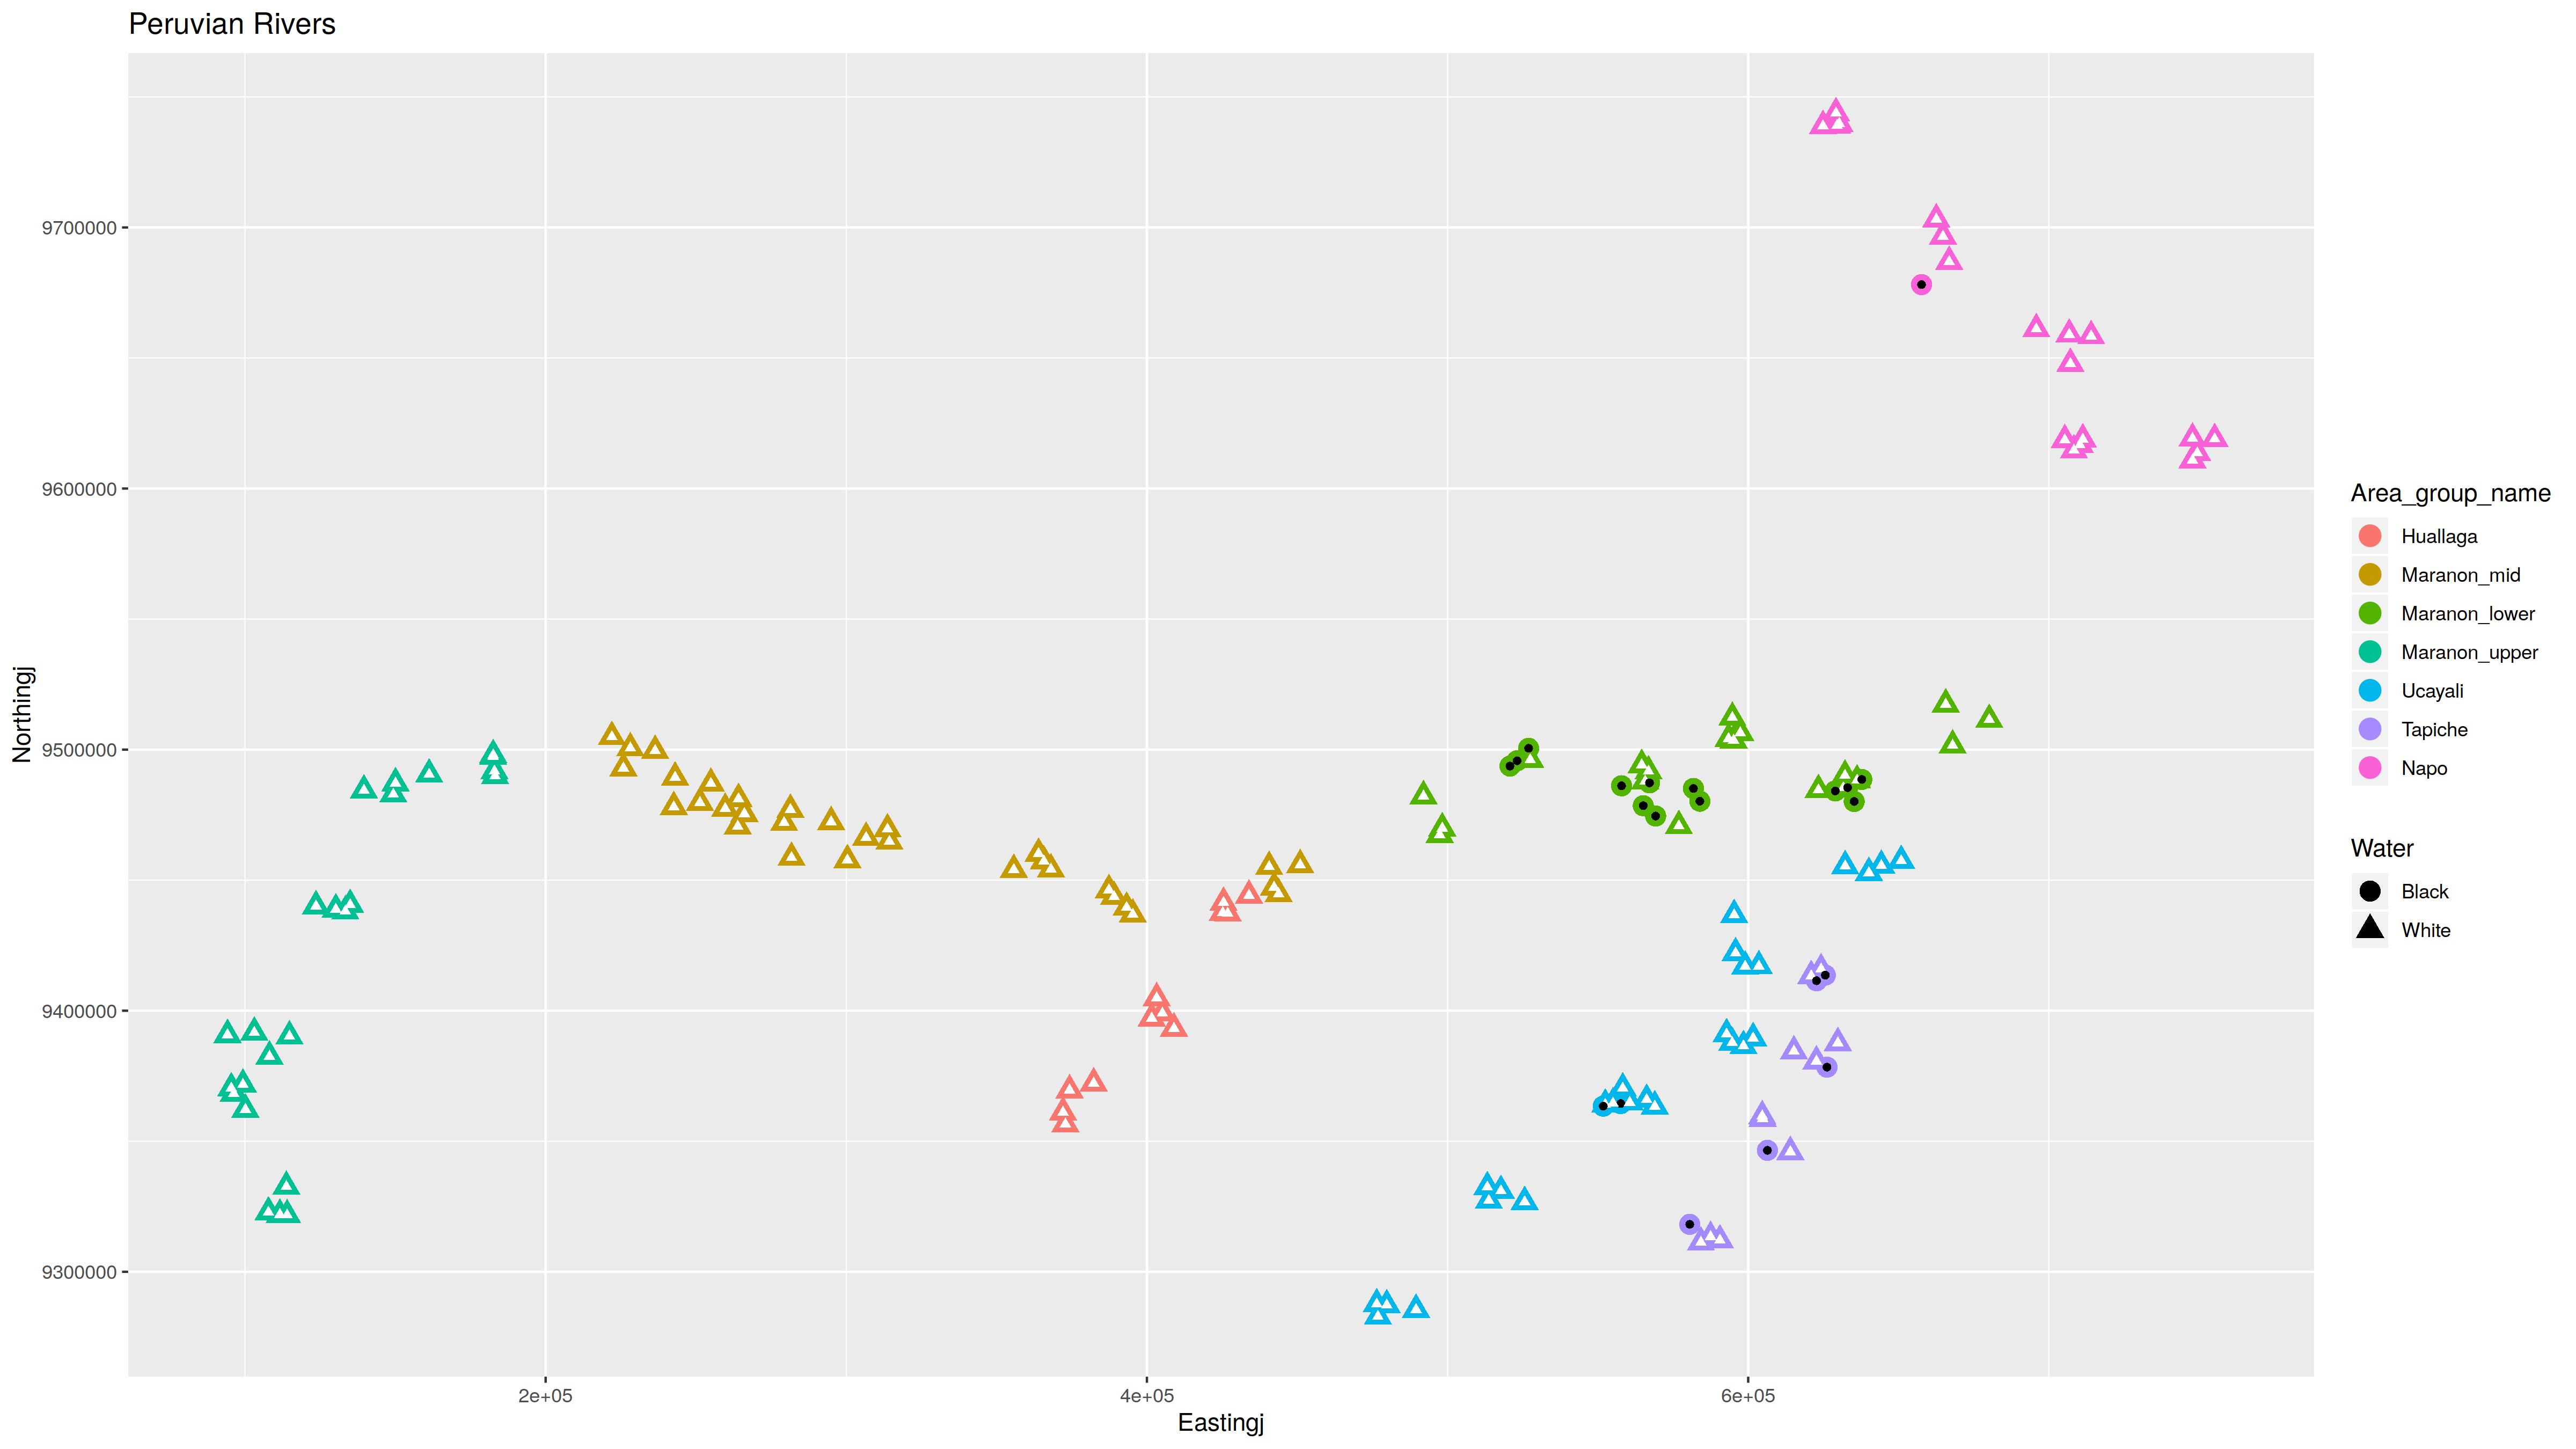
\includegraphics[width=0.7\textwidth]{mapofrivers}
	\caption{A plot of the Easting and Northing coordinates of the samples collected. Colours represent the rivers, and shapes the water colour (triangle for White and circle for Black). The points are also coloured white and black in the middle to aid in viewing. White noise with a standard deviation of $5 \cdot 10^3$ was added to the coordinates so as to separate points close together.}
	\label{fig:graphmap}
\end{figure}
\subsection{Sampling and Preprocessing}
%how data are sampled
The water samples were collected from the sides of a boat using kits provided by NatureMetrics. A volume of water, between 0.5-2L is filtered through a membrane which is then send to the laboratory for DNA extraction. From each site in the river (boat stop), 4 samples were collected (with some sites having a bit more). Information about the sites and samples was also recorded in the metadata (like ID, location, water colour, trip number and date of collection). 

At the laboratory, DNA trapped inside the membranes is extracted and then PCR amplified. The DNA fragments produced are then sequenced using high-throughput sequencing technology that can handle multiple samples at once. The raw reads from the sequencing are processed (filtered and assembled) and then clustered into OTUs with a similarity cut-off point of 99\%. The representative sequences, or the most abundant individual sequences per OTU, were used for taxonomic assignment. After removing not identified we were left with 675.

Five taxonomic Classes were kept for our analysis: Actinopterygii (fish), Amphibia, Aves (birds), Mammalia, and Reptilia. The most instances of OTUs found belonged to the Actinopterygii class, and within that, Siluriformes and Characiformes are the most abundant Orders. Class and Order distributions of OTUs can be seen in Figure \ref{fig:distr}. The sample-OTU table produced was very sparse (meaning that a significant number of entries were 0), as is the case for most studies using metabarcoding techniques. 
%PCR
%Next Generation sequencing
%Biases that come with sampling
%Removal of unidentified species
\begin{figure}[h]
	\centering
	\begin{subfigure}{0.45\textwidth}
		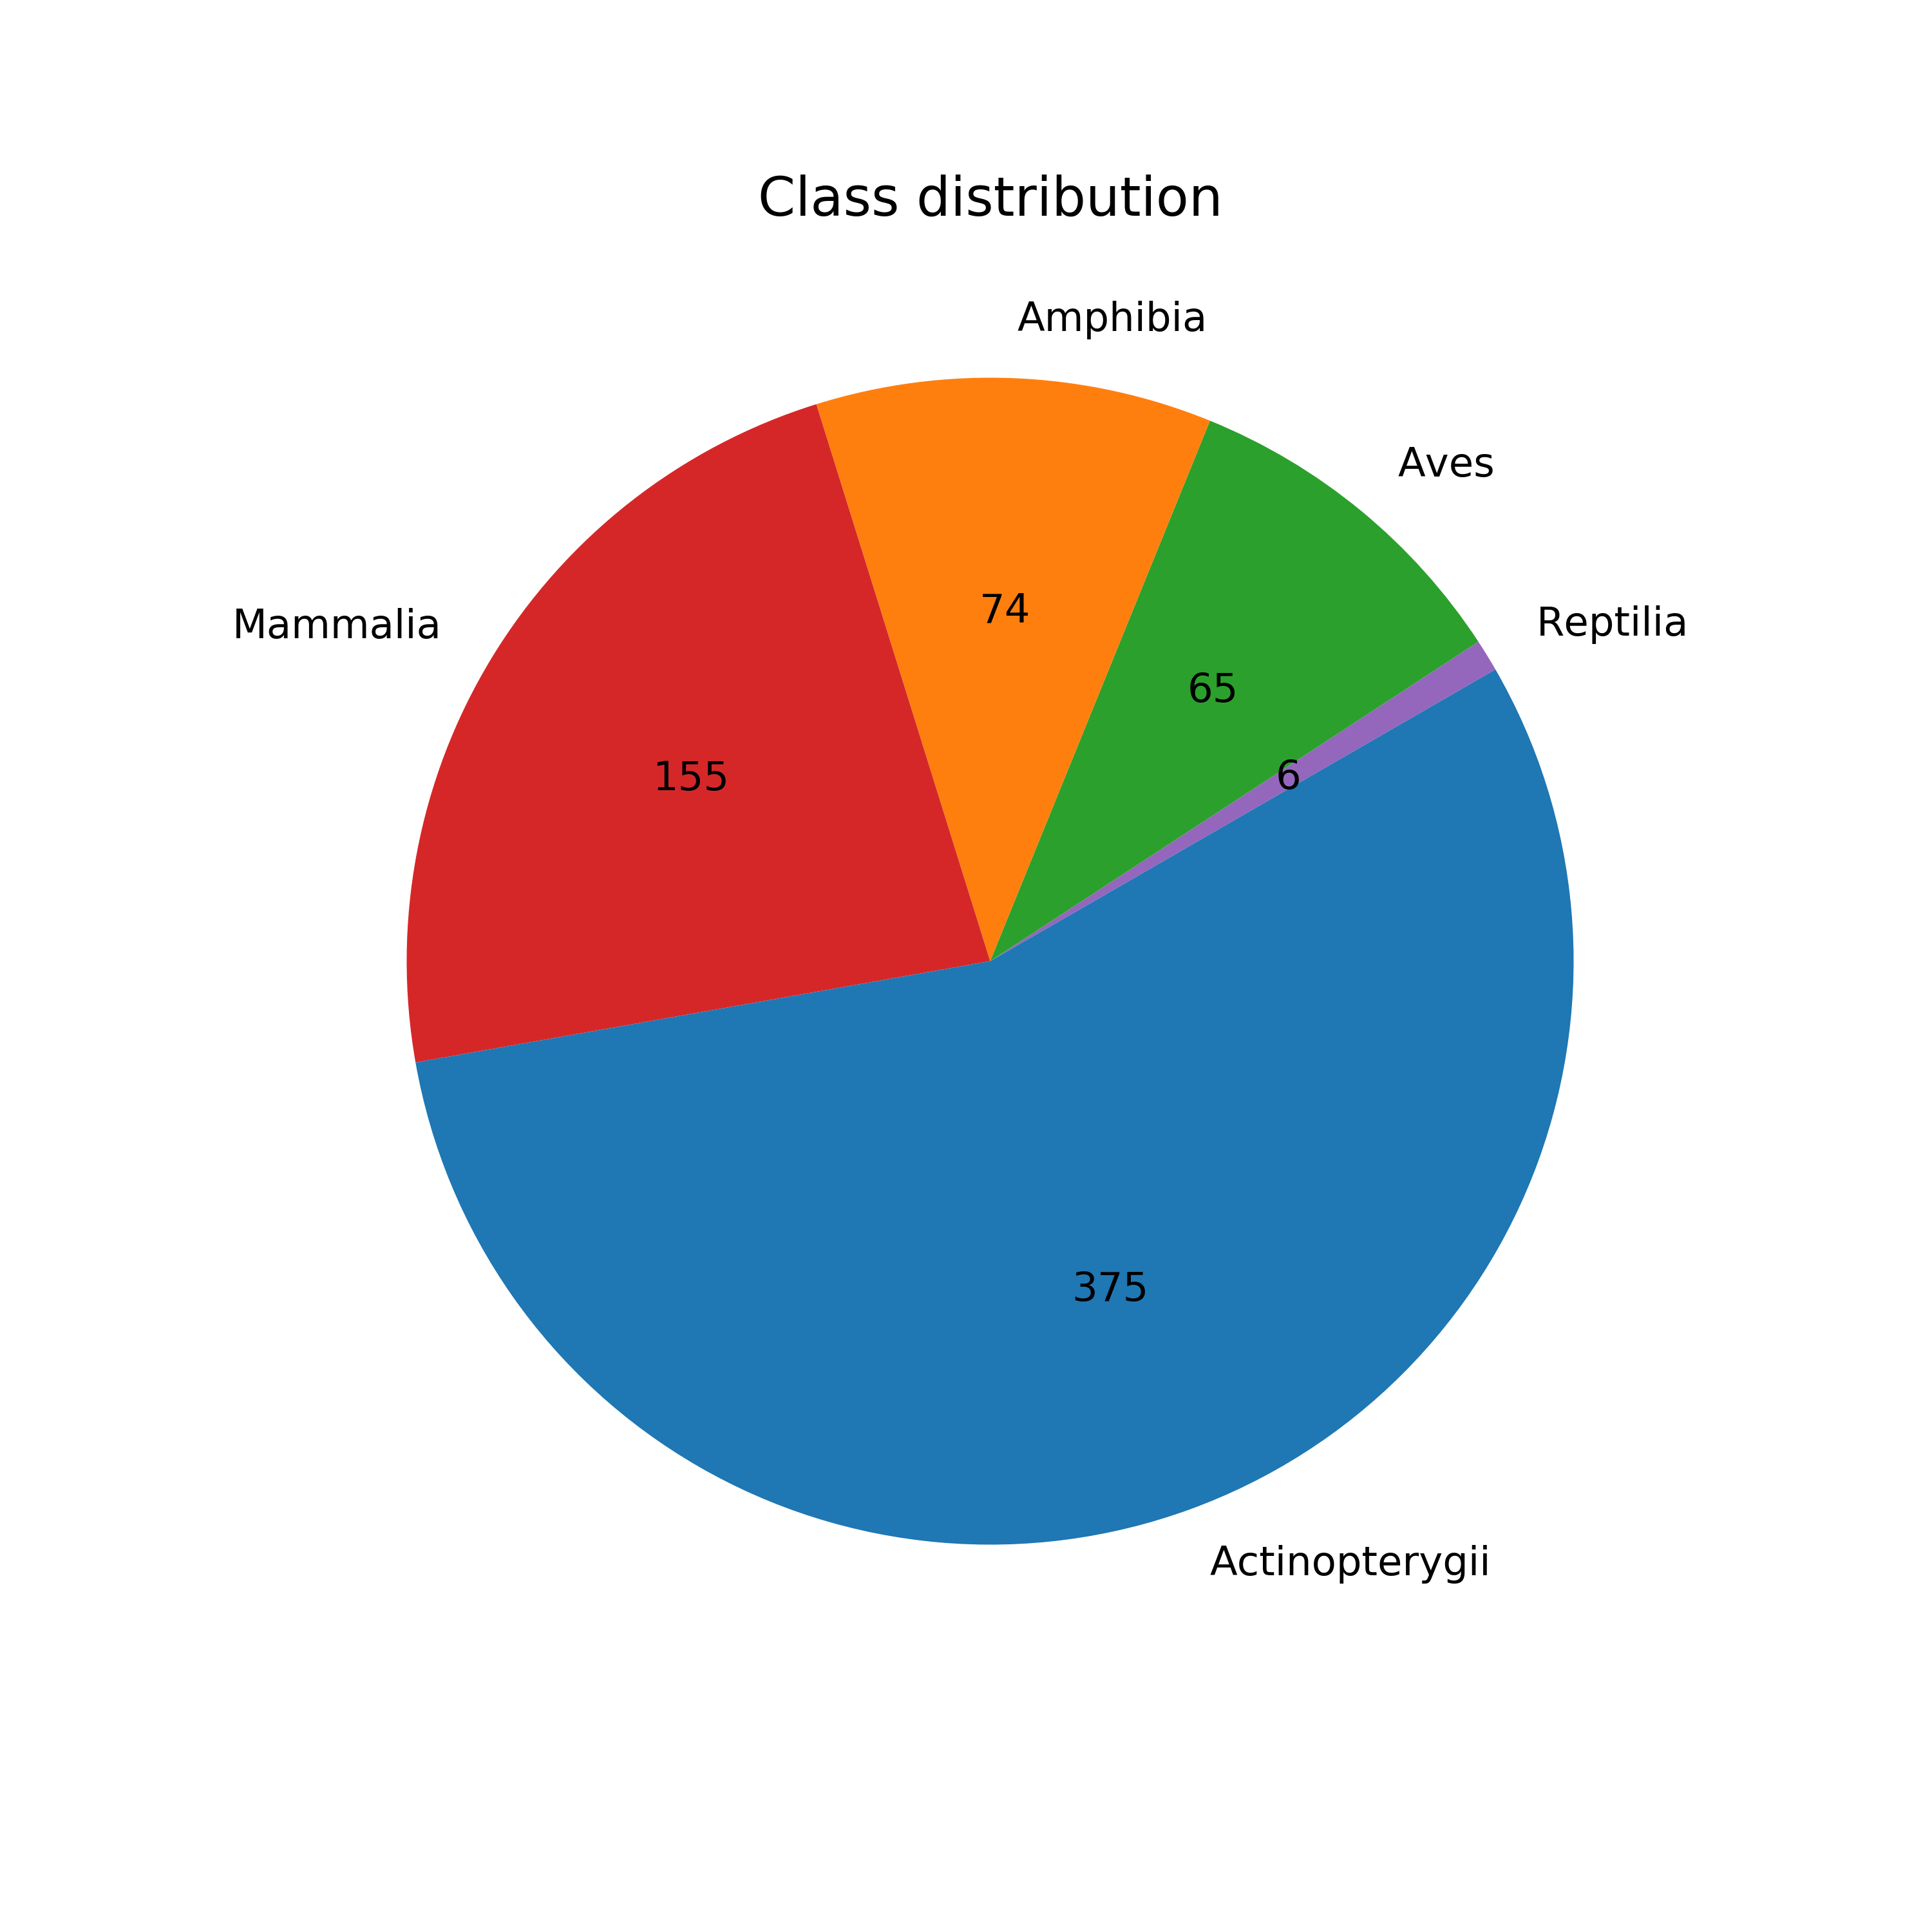
\includegraphics[width=\textwidth]{classdistrpie}
		\caption{Distribution of OTUs into Classes. Most abundant one is Actinopterygii.}
		\label{fig:classpie}
	\end{subfigure}
	\begin{subfigure}{0.45\textwidth}
		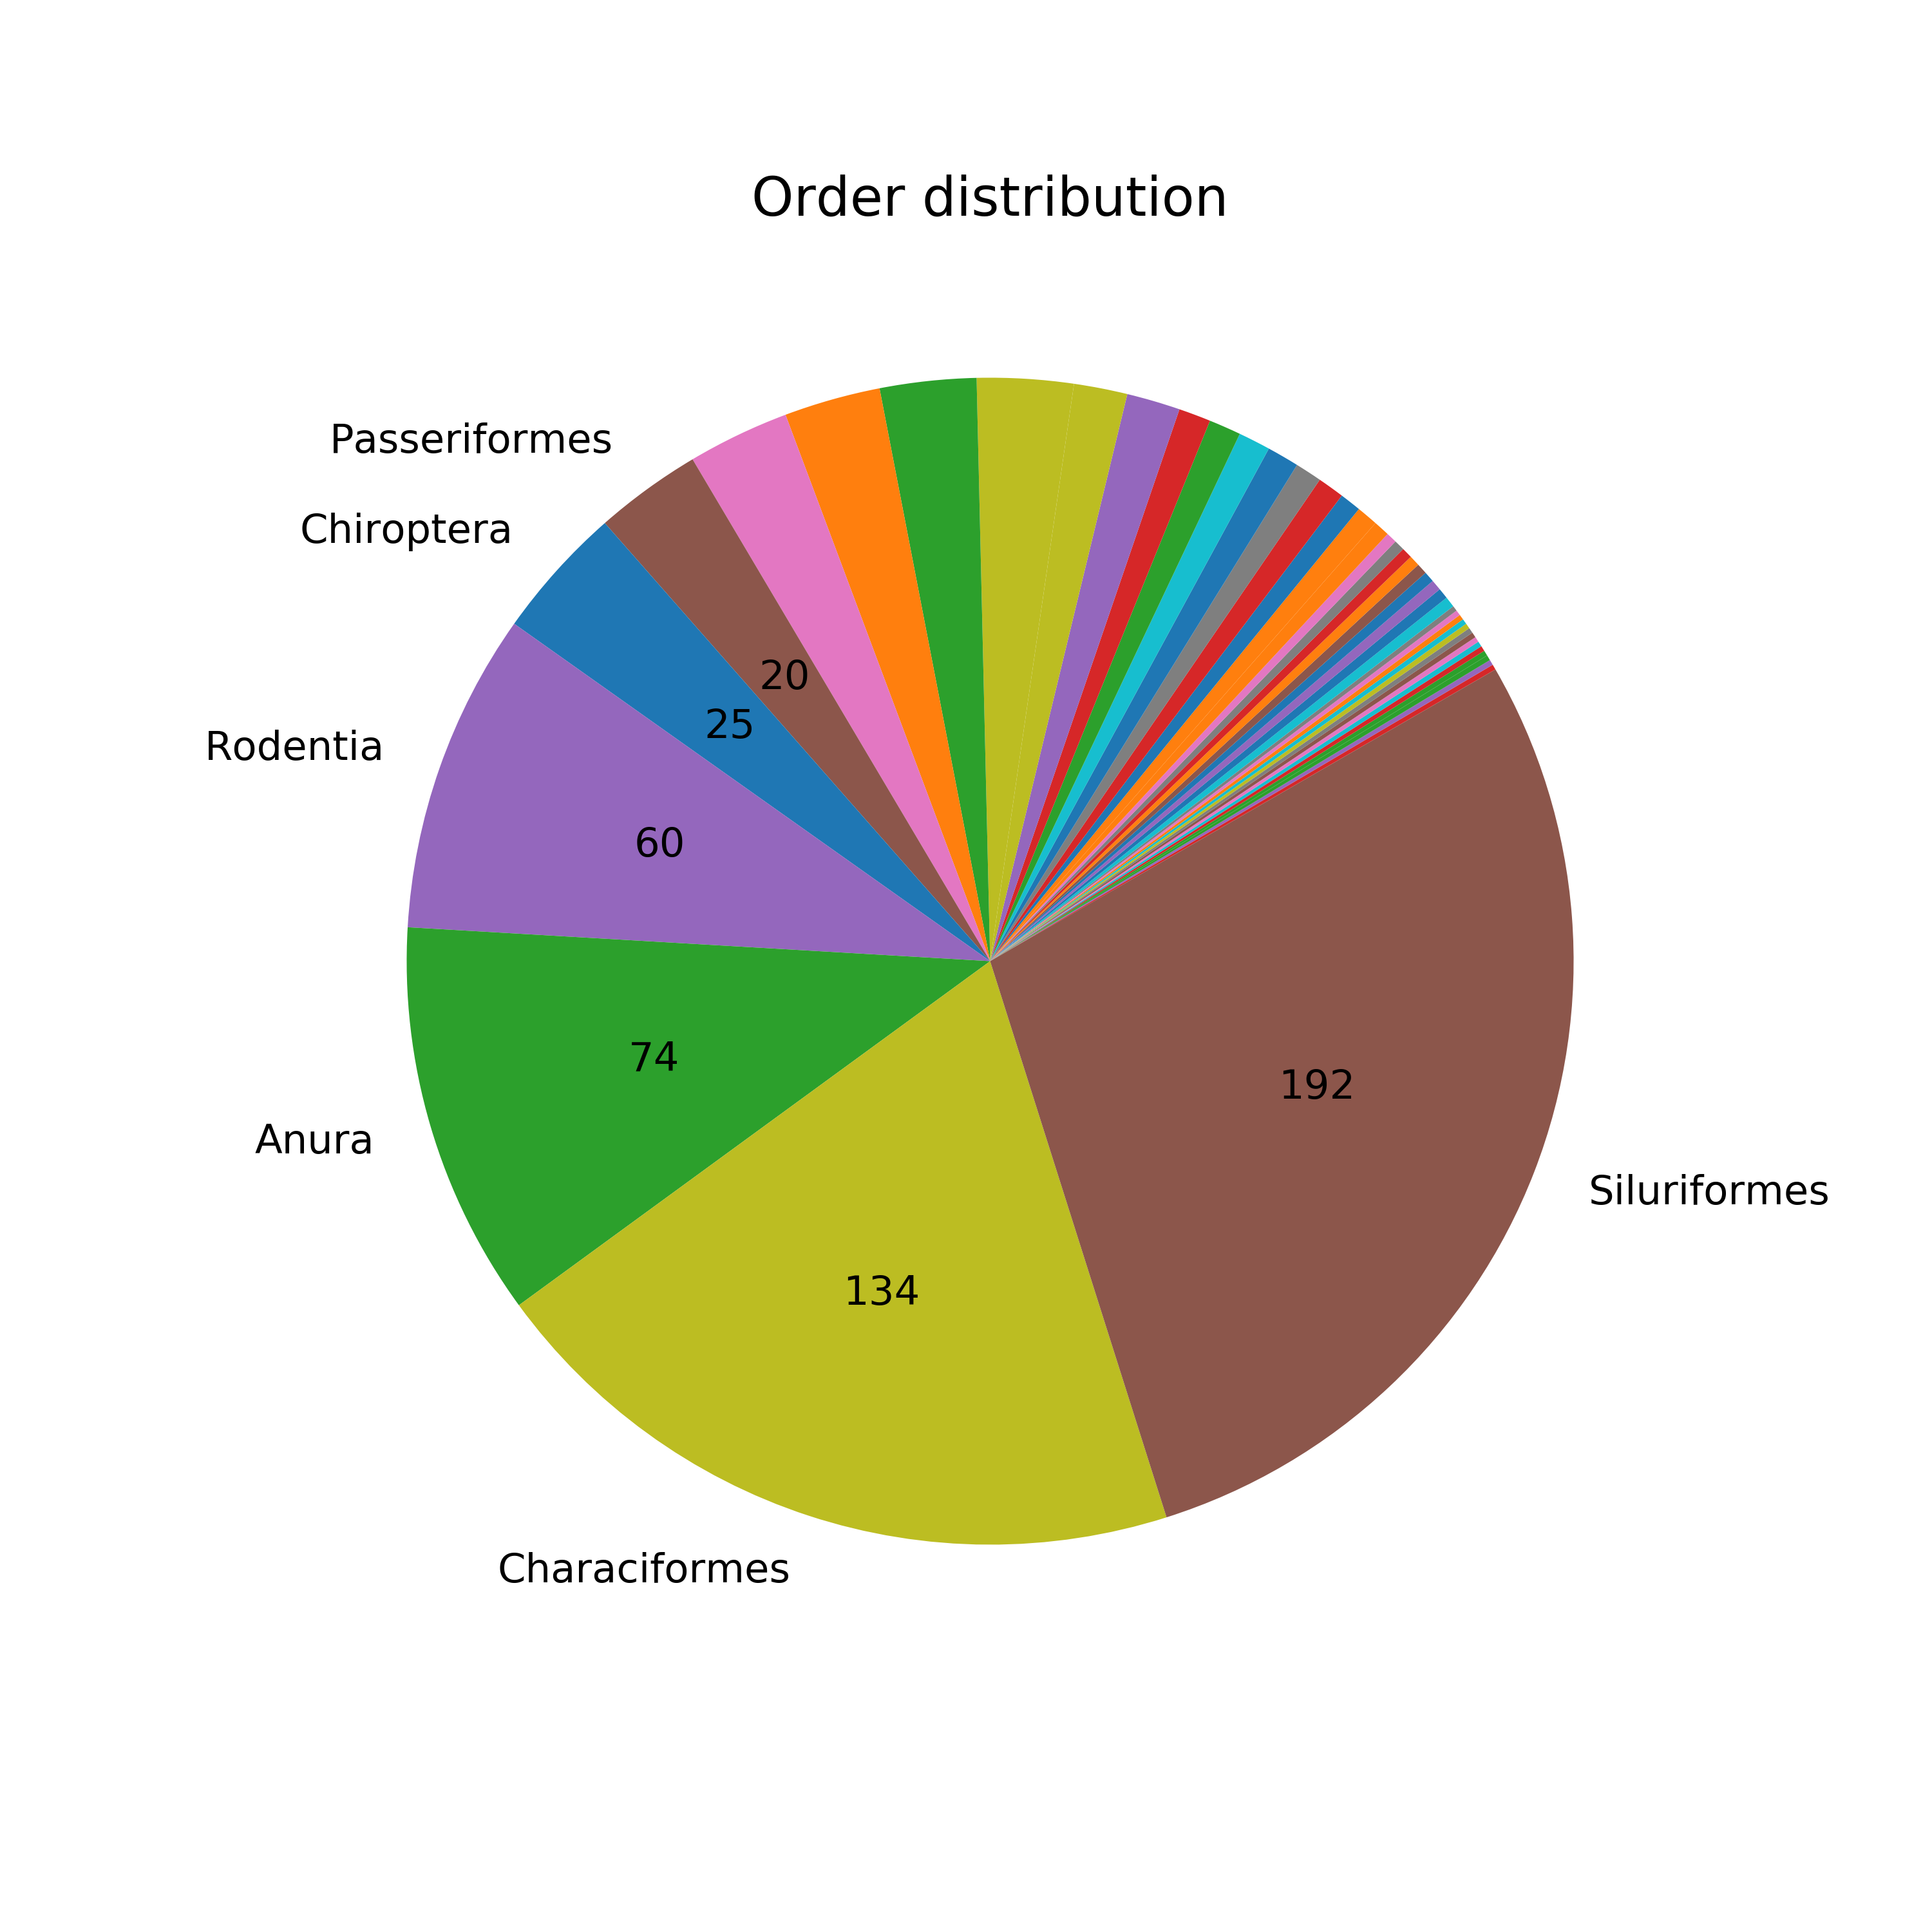
\includegraphics[width=\textwidth]{orderdistrpie}
		\caption{Distribution of OTUs into Orders. Most abundant ones are Siluriformes and Characiformes}
		\label{fig:orderpie}
	\end{subfigure}
\label{fig:distr}
\end{figure}

The sampling methods employed to produce our data come with some inherent biases. First of all, species give out different amounts, sizes and kinds of material behind that can be used to identify them. Furthermore, environmental DNA extracted from the samples can be PCR amplified at different rates for species. This can happen because of primer mismatch with the organisms barcode DNA region. The results can be OTU reads that do not correlate well with the actual abundance of organisms in the environment and also not informative comparisons between OTUs' reads \cite{abundance_nodate}. 

Finally, the OTU table sparsity causes the reads to be concentrated on some samples only, with others having a much lower total read count (sum over the reads of all OTUs in a sample). There are 7 samples (all from white water parts of the river) with under 10000 reads, of which 3 have less than 50. On the other hand, the sample with the largest total counts has 219113 reads. 



\section{Literature Review}
%What has been done by others with data like ours
The advent of metagenetics has opened up the gateway for data driven research in multiple fields. From cataloguing micorbial genes in the human gut \cite{dos_santos_human_2010}, to ecological assessment of freshwater \cite{apotheloz-perret-gentil_taxonomy-free_2017} and river systems \cite{chariton_ecological_2010} using eDNA metabarcoding. Ecological monitoring has traditionally been done using the morpho-taxonomic identification of species in the environment studied. This involves identifying an organism up to a certain level and then using their presence in the site to come to conclusions about the health of the system.


Biotic indices are used to encapsulate information about the abundance of species identified in a site, and also indicate the degree to which a site is healthy. They are highly specialised in what type of pollution they can quantify and which species they consider as important \cite{washington_diversity_1984}. To calculate the value of a biotic index, the species found in a site are assigned a weight (or tolerance value) provided by the index and defined from empirical and experimental data \cite{borja_marine_2000}. Weights signify how susceptible an organism is to the pollution studied \cite{carter_chapter_2017}. Then an analytic formula uses the species weights to calculate the index's value which indicates the environmental quality of the system (usually in categories ranging from `very poor' to `very good').

As mentioned previously, the morpho-taxonomic identification of species is time consuming, expensive and limited in scope. Instead, a metabarcoding approach can generate an OTU table with assigned taxonomy from reference databases in significantly less time. The OTU reads can then be used to calculate biotic indices and evaluate the system's environmental health  \cite{lejzerowicz_high-throughput_2015}. Due to a lack of phylogenetic resolution and limited reference libraries, most metabarcoding data are not used in the calculation of indices. However, taxonomy-free approaches can be used to calculate proxies of biotic indices that have similar evaluation performance \cite{apotheloz-perret-gentil_taxonomy-free_2017}. 

One such approach to calculating biotic indices is through the use of supervised machine learning (SML). The first time that it was employed for biomonitoring surveys was in 2015 by Smith et al \cite{smith_natural_2015} (using microbial eDNA) and in 2017 by Cordier et al \cite{cordier_predicting_2017} (using eukaryotes eDNA). Cordier et al trained two SML models (Random Forests and Self Organising Map) to infer several Biotic Indices used often for marine studies. The features where OTUs reads obtained from foroamfinera eDNA sampled from the benthic zone (sediment on the bottom of the river) and processed in a similar way to the one outlined in the previous section. A notable difference is that unassigned OTUs (without taxonomy) were kept and used as features. Furthermore, the authors constructed new feature data sets using standard ecological techniques such as rarefying and alpha diversity metrics. Target values (biotic indices) were calculated using morpho-taxonomic data and associated weights. 

The SML models performed better in predicting the Biotic index of a site than a reference model that used the taxon assignments of OTUs and a correlation approach for assigning them weights. Also notable is that the SML models had a very high degree of agreement with the morpho-taxonomic evaluation of habitat quality. Furthermore, discarding low abundance OTUs (low total read counts across samples) did not affect the models' performance. The researchers followed up their paper with a more comprehensive one in 2018 \cite{cordier_supervised_2018}, which tested their SML methods on OTUs derived from 5 different ribosomal bacterial and eukaryotic markers\footnote{These markers are specifically designed to amplify regions of the genome that would be used in the identification of species. Multiple exist because of the different regions in the DNA needing to be amplified for the identification of specific groups of organisms (like eukaryotes and bacteria).}. They found that there was no significant difference in the models' performance when using different markers, and that for all of them, SML outperformed all taxonomy-based eDNA biomonitoring methods. 



Usually, analysis of metabarcoding (OTU reads per sample) or metagenetic (genes per sample) studies does not involve machine learning approaches. Researchers analyse alpha (within) and beta (between) diversity metrics of samples (see Figure \ref{fig:otu}), explore the patterns in beta diversity using ordination techniques, and perform various classical hypothesis tests. 

\begin{figure}
	\centering
	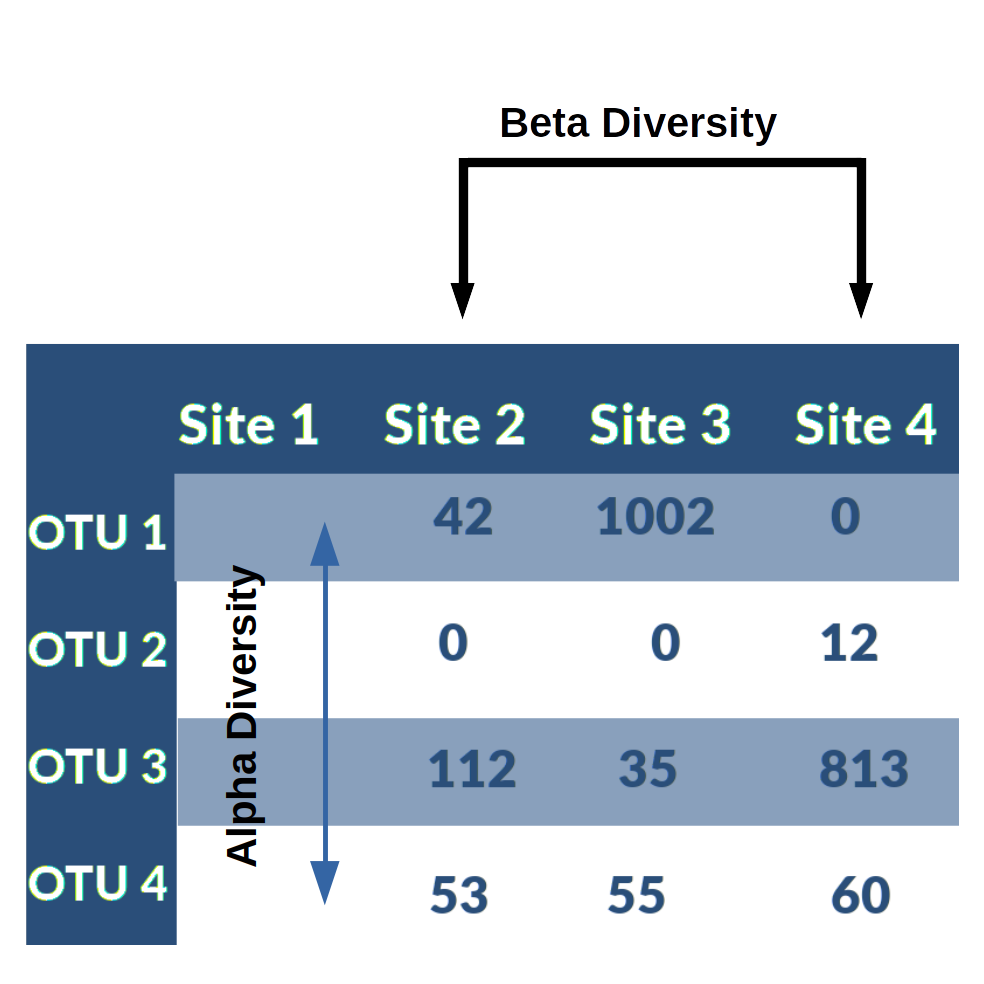
\includegraphics[width=0.5\textwidth]{otutable}
	\caption{An illustration of Alpha and Beta diversity metrics as calculated from OTU tables}
	\label{fig:otu}
\end{figure}

Alpha diversity metrics are a measure of the diversity a sample displays within itself (with respect to the OTUs' reads). An example can be OTU richness which measures the number of OTUs present in the sample (without taking into account the reads) or Shannon index which converts the reads into probabilities (by dividing them with the sample's total reads) and calculates the sample's entropy. The formula is given by:
$$-\sum_{i=1}^s p_i \ln(p_i),$$
were $s$ are the number of species present in the sample, and $p_i$ is the read count of the $i$th OTU divided by the total read count of all OTUs in the sample. 

Beta diversity measures how different samples are in terms of their species composition. They usually take the form of (dis)similarity measures, and some of the more common ones used are Bray-Curtis, Chao and Jaccard (to be explained later). The output of these measures is a symmetric matrix whose elements quantify how (dis)similar the samples are. Ordination methods can then be applied to this matrix that explore its structure graphically. Environmental variables, like pH, concentrations of minerals, or pollutants, can be fitted on top of these plots and help researchers uncover patterns in OTU composition that explain the variables' variation.

If there is a discernible pattern in the ordination plots of the data that separates them along a gradient or grouping of a variable, then differential  abundance analysis can be used to investigate it further. For example, if samples are separated into two groups that also happen to coincide with a categorical variable of the data, a model can be fit to test which OTUs are differentially abundant across the grouping that causes the separation. Parametric models include Zero-Inflated Gaussian mixture model,   Zero-inflated Log-Normal mixture model \cite{css_diff_abund}, and other generalised linear models (like overdispersed Poisson model) \cite{robinson_edger:_2010}. The choice of distributions to model read counts is highly dependent upon the problem and also very debatable \cite{css_diff_abund,white_statistical_2009,mcmurdie_waste_2014}; if their assumptions about the data are not met they can yield a high level of false negatives/positives. 

Non-parametric tests exist that test if groupings of samples (that divides them into two or more groups) result in populations that have significantly different distributions. Such tests include the Mann-Whitney test and permutational multivariate analysis of variance (PERMANOVA). To use such tools the data have to be transformed in some way first, either using alpha or beta diversity. 
%%\textbf{Alpha and Beta Diversity metrics}
%\url{https://www.drive5.com/usearch/manual/diversity_metrics_recommended.html}
%Alpha diversity is the species diversity in a single ecosystem or sample. The simplest measure is richness, the number of species (or OTUs) observed in the sample. Other metrics consider the abundances (frequencies) of the OTUs, for example to give lower weight to lower-abundance OTUs.  
%Beta Diversity measures the differentiation of species diversity between samples or habitats. 
%
%\textbf{Bray–Curtis dissimilarity statistic}:
%In ecology and biology, the Bray–Curtis dissimilarity, named after J. Roger Bray and John T. Curtis,[1] is a statistic used to quantify the compositional dissimilarity between two different sites, based on counts at each site. \url{https://en.wikipedia.org/wiki/Bray%E2%80%93Curtis_dissimilarity}
%	
%	The \textbf{Shannon index} is an information statistic (alpha diversity) that measures diversity of species in a sample. It assumes that all species are represented in the sample and are also randomly sampled. It's equation is given by
%	$$-\sum_{i=1}^s p_i \ln(p_i),$$
%	where $i$ is the index of one of the $s$ species in the sample, and $p_i$ is given by $\frac{n_i}{N}$ where $n_i$ is the number of individuals $i$ in the sample of $N$ individuals.
%	
%	The \textbf{Simpson Index} is a dominance statistic (alpha diversity) that gives more weight to more common species found in the sample. It can be thought as measuring the `effective' number of species and is given by
%	$$\frac{1}{\sum_{i=1}^s p_i^2}$$the value of $p_i$ is defined in  the same way as in the Shannon index.
%	The  \textbf{Jaccard Index} (beta diversity) measures how similar, in terms of species present, two samples are. It ranges from 0 to 1, with the latter indicating that the two samples share the same species. The index does not take into consideration the abundance of species. It is given by
%	$$\frac{|X \cap Y|}{|X\cup Y|},$$
%	where $X$ and $Y$ are two samples, whose intersection is the number of species shared between them and their union is the the total number of species across them.
% Ecological assessments of such surveys have generally been restricted to measuring taxon relative abundances, analyzing within- and between-sample diversity (α and β diversity, respectively), exploring β-diversity patterns using unsupervised learning techniques such as clustering and principal coordinates analysis (PCoA), and performing classical hypothesis testing. These approaches may be limited in their ability to classify unlabeled data or to extract salient features from highly complex and/or sparse data sets. knights et al 2011

%Talk about alpha beta diverrsity and how ordination is used. Also how different abundance testing is done (FitZig) and cite packages used (vegan metagenomeseq DESkati)
%machine learning to characerise biotic index of rivers

\section{Aim}

The aims of this project are to explore the data set obtained from eDNA metabarcoding of samples collected from Peruvian rivers, and use the OTU table to predict the water colour of samples. Data processing techniques like feature selection through correlation and normalisation of the read-counts will be presented in Chapter \ref{chap:data}. These modifications to the OTU table will be used as new features for the classification of samples. Their spatial distribution along the rivers will be taken into account when designing train-validation-test splits; we designed different conditions under which the models'  weaknesses and strengths could be uncovered. These are outlined and explained in the Chapter.

Ordination methods will be used with a variety of distance measures to identify patterns in the data. These methods can also be used for dimensionality reduction, and thus more features will be created for classification. An introduction to the most popular ordination methods will be presented in Section \ref{sec:ordination}. Also, it will be proven that Principal coordinate analysis is a general case of Principal components analysis.

 Permutation Analysis of variance  will be presented in section \ref{sec:permanova}. This classical ecological test hypothesis method  will be used to evaluate if the grouping by water colour divides the samples into populations with significantly different distributions. 

Supervised machine learning models will be trained to predict water colour of samples using a variety of features derived from OTUs. An outline of Bayesian and maximum likelihood logistic regression, as well as of Random forests will be presented in section \ref{sec:classification}. 

These models will then be tested in the ways explained previously, and their performance compared for all the features created. Furthermore, the taxonomic Orders with the most explanatory power will be identified.



%Add packages to all sections like ordination and machne learning
%remove Logistic regression from machine learnig. Start that section with Bayesian framework and then say how logistic regression uses loss functions instead of priors etc.. maybe use AIC as well
%!TEX root = ../thesis.tex
%*******************************************************************************
%****************************** Second Chapter *********************************
%*******************************************************************************

\chapter{Data Processing and Splitting}
\label{chap:data}
\ifpdf
    \graphicspath{{DataChapter/Figs/Raster/}{DataChapter/Figs/PDF/}{DataChapter/Figs/}}
\else
    \graphicspath{{DataChapter/Figs/Vector/}{DataChapter/Figs/}}
\fi



\section{Processing}

In this Chapter, we explore in what ways we can process our data before using them for classification and how we might test our classifiers while taking into account the spatial distribution of the samples. Datasets obtained through metabarcoding or metagenetic methods usually display high variability in read counts between and within samples that stems from systematic biases. Several normalisation techniques have been developed to deal with this issue; we present some of them and  will evaluate their usefulness in classification. Furthermore, inspired by the interdependent nature of species in animal communities, we use correlations between features for feature selection.


The samples' location in the river surely introduces some dependencies between them; animals tend to wander around their habitat, and thus eDNA collected from sites close together will be more similar than those far apart. The way our data is split for training, validating and testing will influence our classifiers' performance. We present two methods of splitting them, using their location as the deciding variable, that will test the classifiers' ability to extrapolate information gained through training. Furthermore, we outline the cross-validation procedure to be used for the evaluation.
\subsection{Normalisation}

Count data from amplicon sequencing display a very high degree of variability in total read counts per sample \cite{inadmissible_rareying}. A histogram, Figure \ref{fig:counthistogram}, of the samples' total count reads for our data exemplifies this variability. The sums range from 17 to 219113, with a median and mean of 63672 and 77152 respectively. This much variation between samples makes it hard to identify which OTUs' difference in abundance between samples is significant and also might negatively impact the performance of the classifiers. 
 
 The increased variation comes from a systematic variability affecting multiple samples and OTUs in a similar manner. Sources of such variability can be the inconsistencies in DNA extraction and handling of samples,  a varying quality of sequencing runs \cite{pereira_comparison_2018}, and other PCR-specific amplification biases (like primer mismatch, GC-content etc.) \cite{abundance_nodate,krehenwinkel_estimating_2017}.
 
 Furthermore, these biases can cause the distribution of read counts obtained from high-throughput amplicon sequencing to diverge significantly from the actual distribution of species abundances inhabiting in the same regions where the samples were collected. The Pearson correlation between read counts and actual species frequencies is close to zero \cite{edgar_unbias:_2017}.
 
 The removal of this systematic variability is called \textit{Normalisation} and it's original aim in the bioinformatics literature is to increase the statistical power and false positive rates of differential abundance analysis \footnote{Differential abundance analysis aims at finding OTUs (or genes in the case of metagenomic studies) whose variation between groups of samples (e.g. black and white water river samples) is statistically significant.}. We will be testing if normalisation methods have any effect on the classifiers' scores.
 
 A normalisation method that produced promising results in differential analysis on datasets similar to ours is Cumulative sum scaling (CSS). This method is an extension to the quantile normalisation approach which divides read counts by the $Q$th percentile of each sample’s non-zero count distribution. CSS determines that percentile using a data-driven approach \cite{css_diff_abund}.
 
 To illustrate how normalisation methods work we define $X_{i,j}$ as the read counts of sample  $i =1,...,n$ and OTU $j=1,...,p$. The normalisation factor of the total sum scaling (TSS) method is found by summing the read counts in a sample $i$:
 \begin{equation}
 	N_i = \sum_{j=1}^{p} X_{ij}.
 	\label{eq:totalsum}
 \end{equation}
Then the counts in row $i$ of the read matrix $X$ are divided by the factor $N_i$. TSS is the most commonly used method of normalisation but it has been shown to introduce biases in differential analysis estimates \cite{bullard_evaluation_2010}.

Quantile scaling computes the normalisation factor by taking into account how OTU total counts (for all samples) vary, and choosing a percentile that produces desirable properties (such as robustness from highly abundant OTUs).
The scaling factor is defined as:
\begin{align}
	N_i &= \underset{ j \in G}{ Q\text{th quantile}} \  X_{ij}\\
	G  &= \left\{ j : \sum_{i = 1}^{n} X_{ij} > 0\right\}.
\end{align}

 
\begin{figure}[htb]
\centering
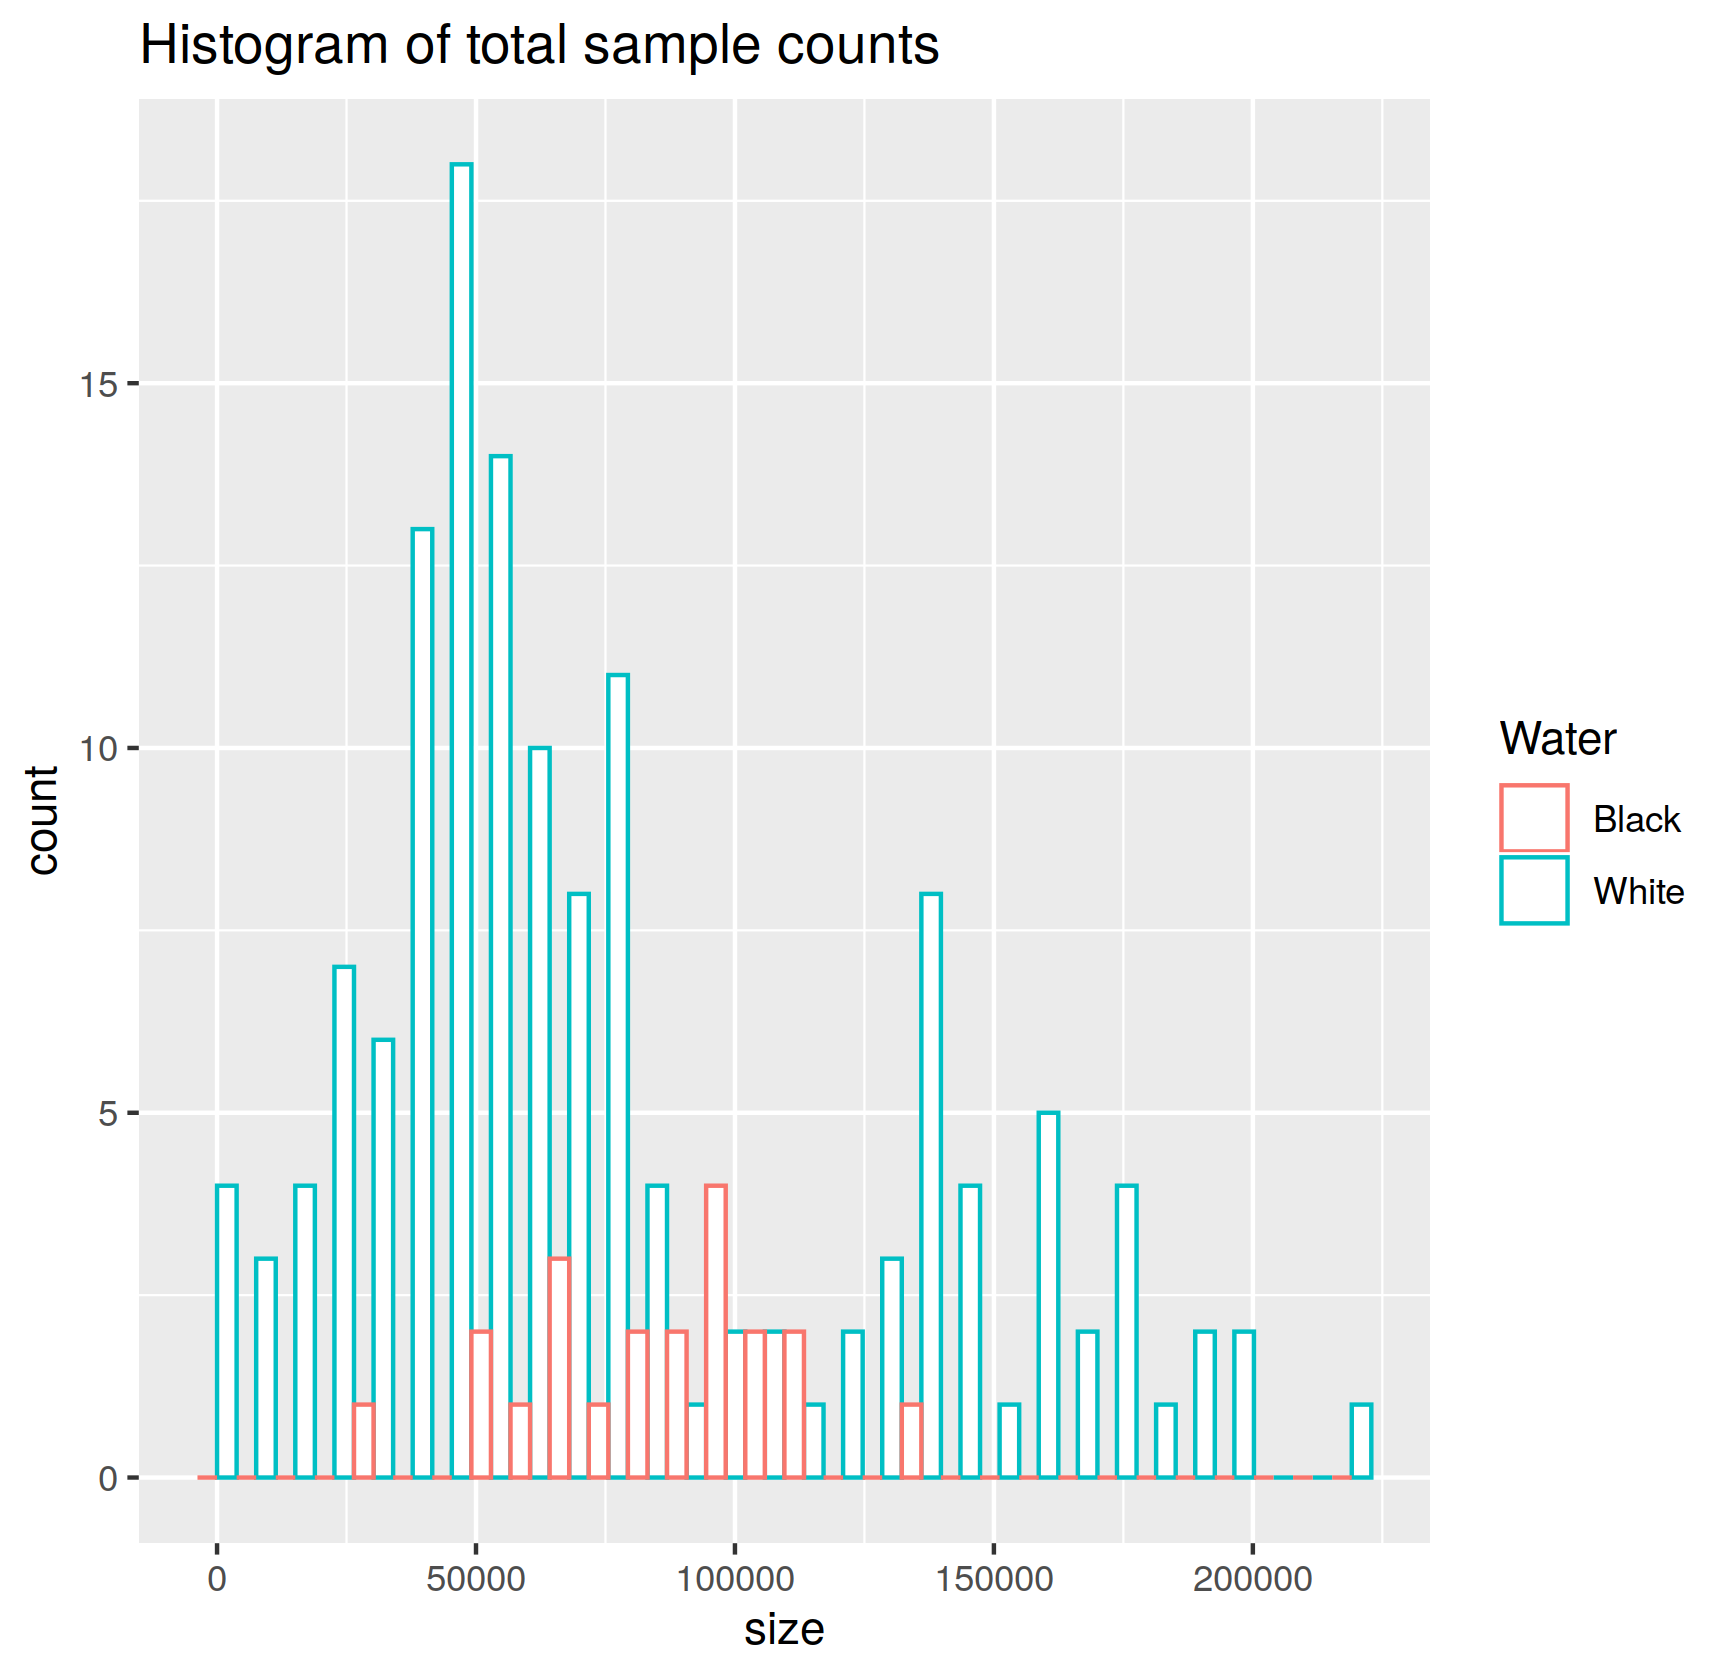
\includegraphics[width = 0.7\textwidth]{histogramofcountdata}
\caption{Histogram of the sum of OTU counts of each sample. The cyan colour represents white water samples and the red colour black water samples.}
\label{fig:counthistogram}
\end{figure}

CSS normalisation involves the calculation of a data-driven quantile 
We define the $l$th quantile of sample $i$ as $q_i^l$, which means that $l$ OTUs have a read count lower than $q_i^l$. Also we define the sum of counts per samples $i$ up to the $l$th quantile as
\begin{equation}
	s_{i}^{l}=\sum_{j|X_{ij} \leq q_{i}^{l}} X_{ij}.
\end{equation} 
With this notation, the total sum normalising factor \eqref{eq:totalsum} is given by $N_i = s_i^p$ (where $p$ is the total number of OTUs). CSS chooses a value $\hat{l} \leq p$ using a data driven approach to calculate the scaling factor ($N_i = s_i^{\hat{l}}$) for each sample and get normalised counts.
In particular, the quantile $\hat{l}$ for the threshold $q_i^{\hat{l}}$ is chosen  to be the smallest value where the median absolute deviation of sample-specific quantiles $q_i^l$ from a reference point (the median quantile $q_i^l$ across all samples) shows high instability. \cite{css_diff_abund}.
% web

% CSS + LOG histograms 
\begin{figure}[h]
	\centering
	\begin{subfigure}{0.4\textwidth}
		\centering
		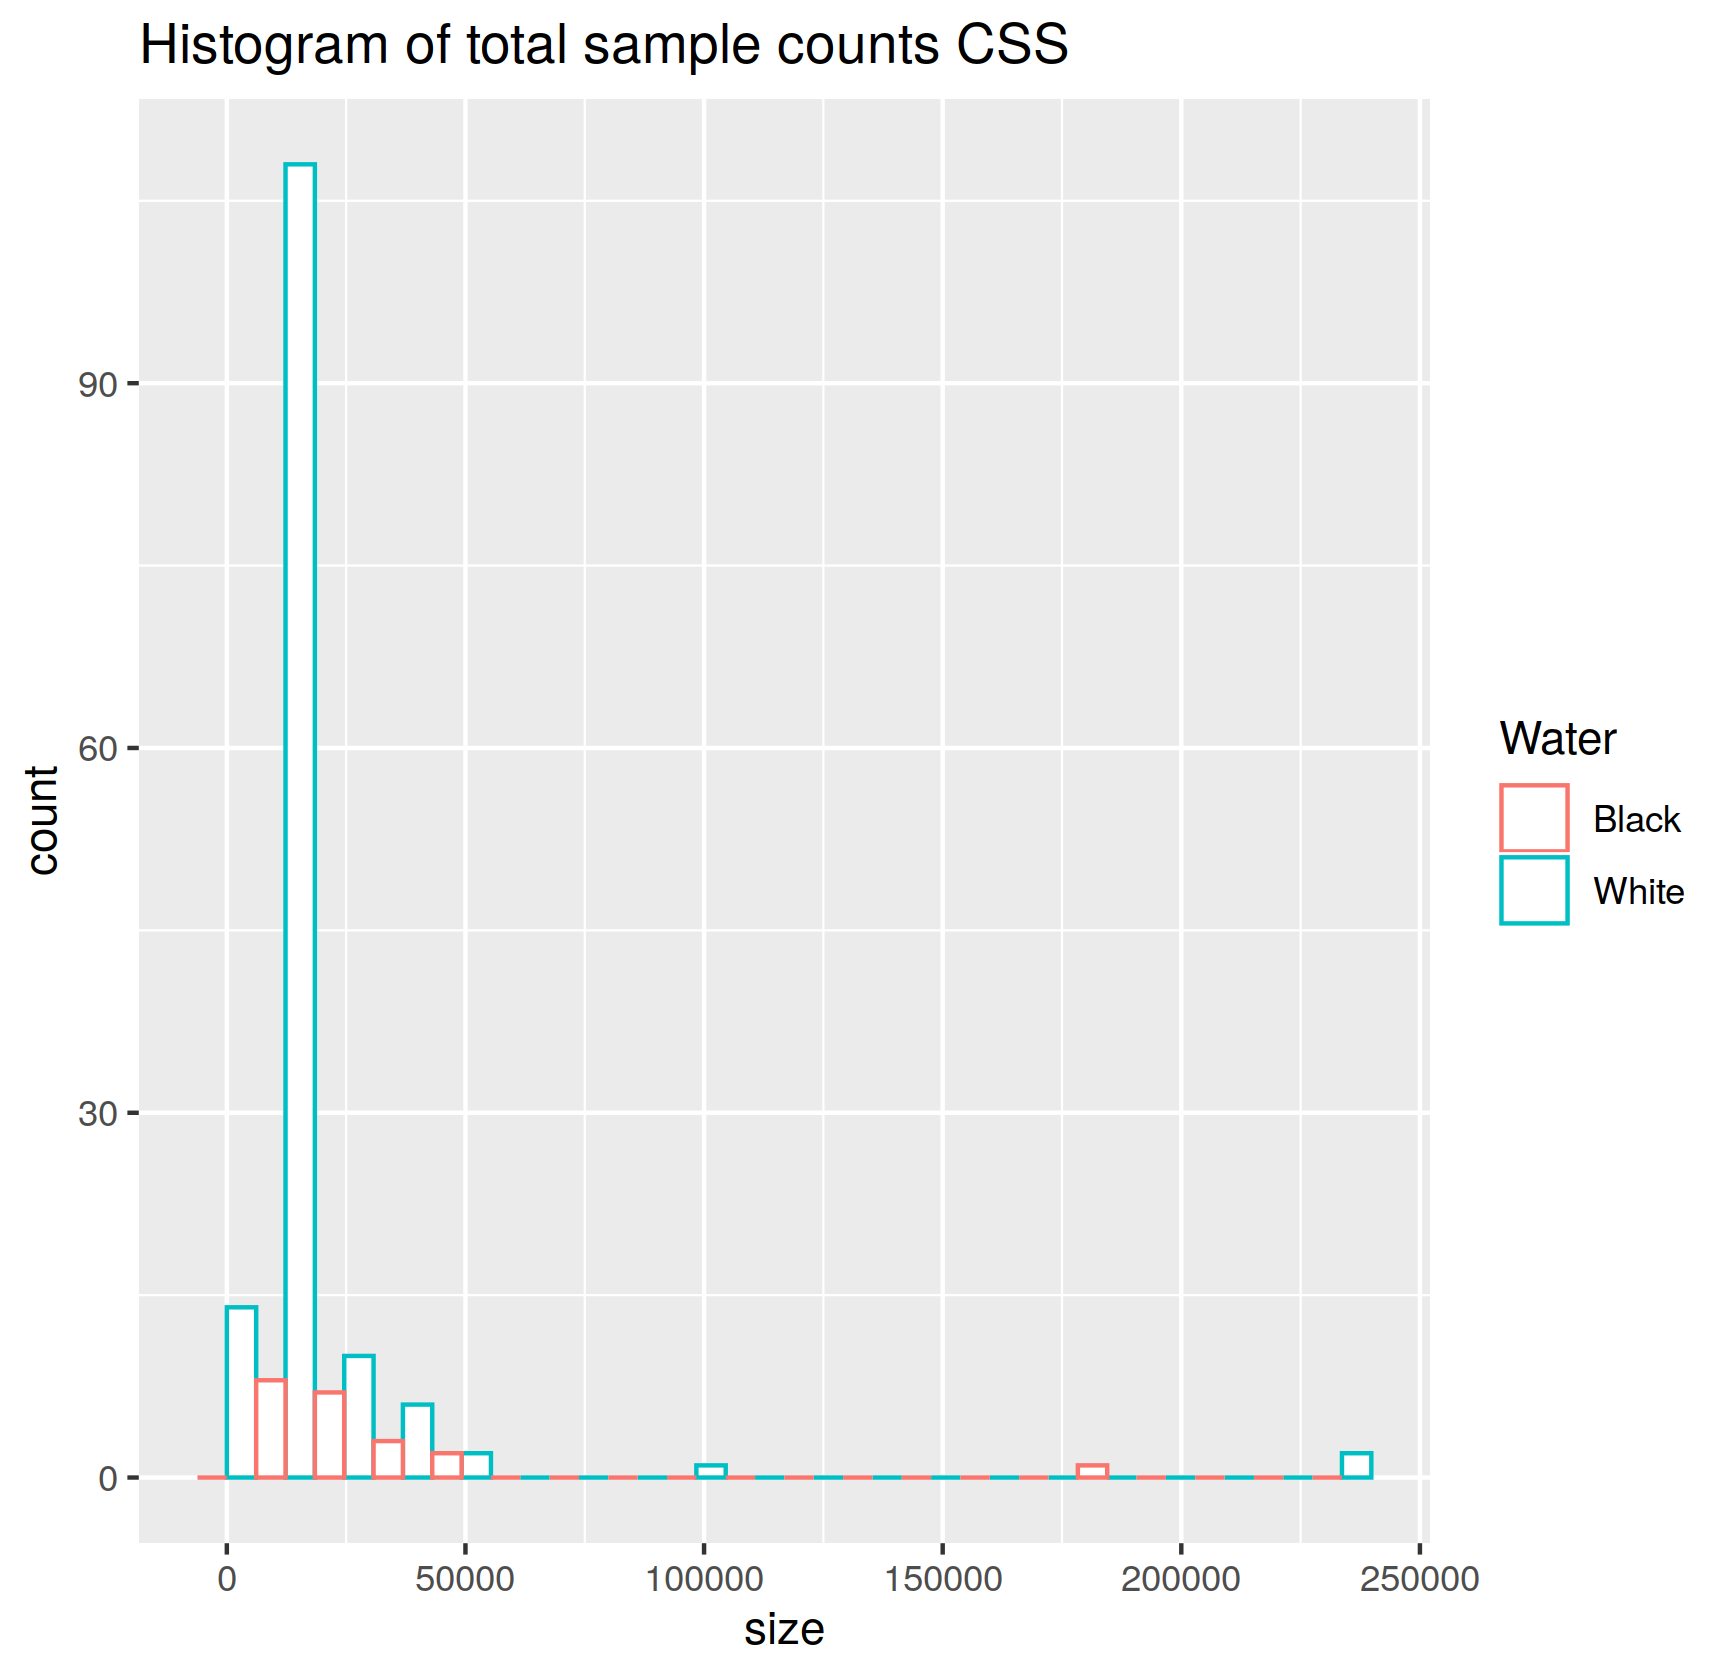
\includegraphics[width = \textwidth]{histogramofcountdatacss}
		\caption{}
		\label{fig:histcss}
	\end{subfigure}
	\begin{subfigure}{0.4\textwidth}
	\centering
	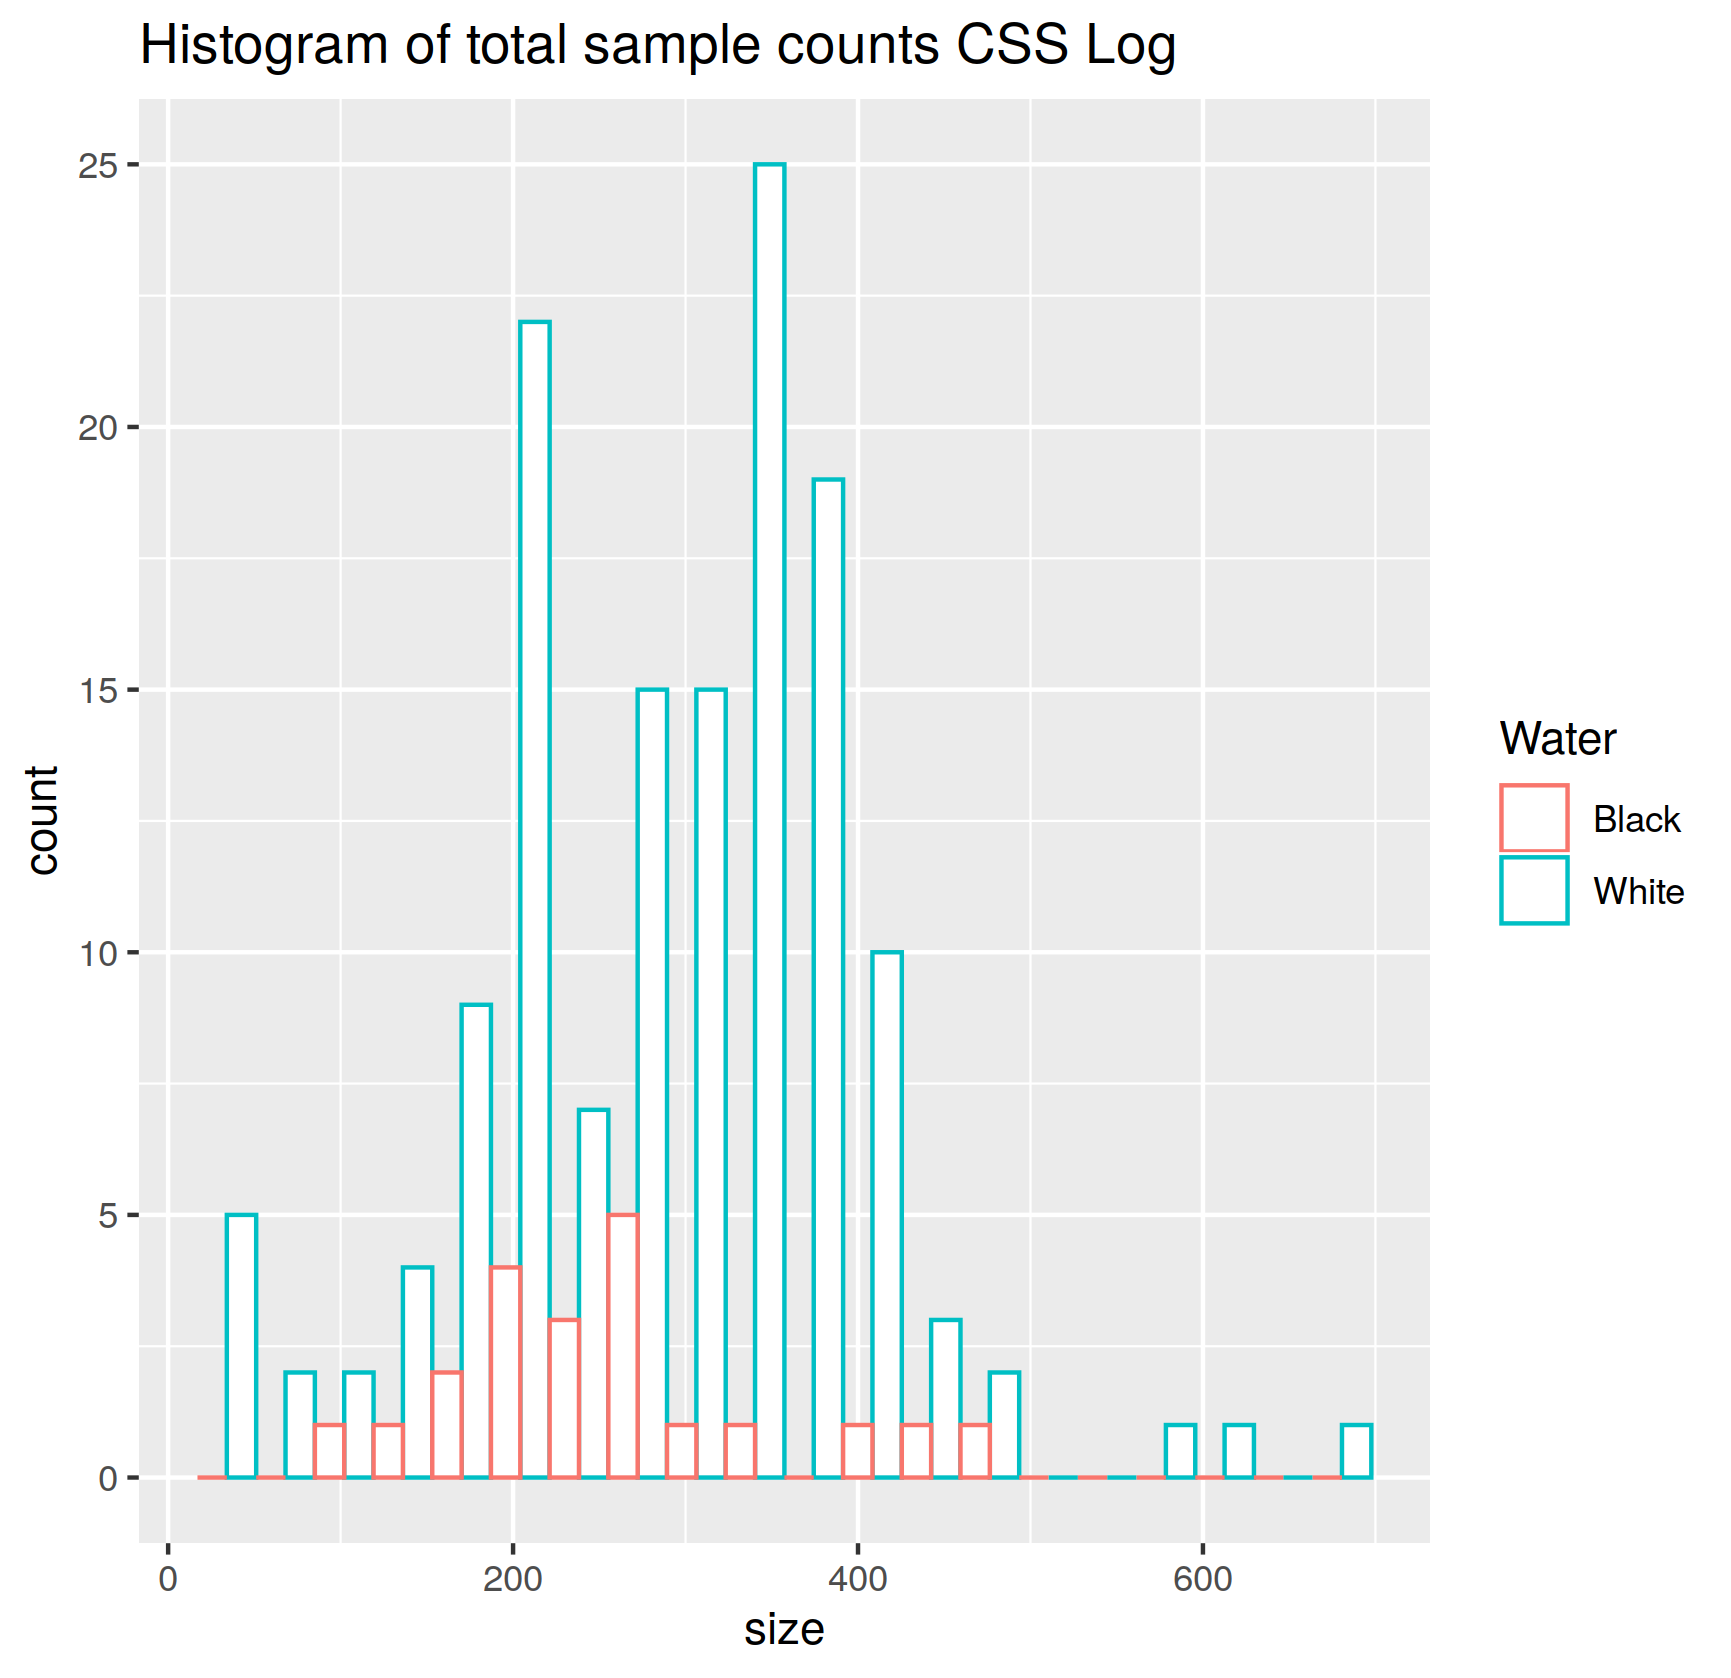
\includegraphics[width = \textwidth]{histogramofcountdatacsslog}
	\caption{}
	\label{fig:histcsslog}
	\end{subfigure}
	\caption{Histogram of the read counts per sample after \ref{fig:histcss} CSS normalisation and with \ref{fig:histcsslog} a $log_2$ transformation. The cyan colour represents white water samples and the red colour black water samples. }
\end{figure}


Using CSS normalisation on our data causes the variation of read counts per sample to drop significantly (except for some samples whose total read counts increase, see Figure \ref{fig:histcss}). Applying a further $log_2$ transformation to the data after normalising reduces the variation even more (see Figure \ref{fig:histcsslog}). The transformation does not apply the logarithm to $0$ valued read counts.  Furthermore, using Principal coordinate analysis and Non-metric multidimensional scaling (Figure \ref{fig:pcoa12otucss} and \ref{fig:nmds12otucss} respectively) ordination on the normalised data separates white and black water samples better than if the normalisation was not applied\footnote{These methods are similar to Principal Components Analysis in that they reduce the dimensions of the data. An outline of their use and how they are performed will be presented in the next Chapter.}. However, doing the same on the $log_2$ transformed data does not have the same effect.

\begin{figure}[h]
	\centering
	\begin{subfigure}{0.4\textwidth}
		\centering
		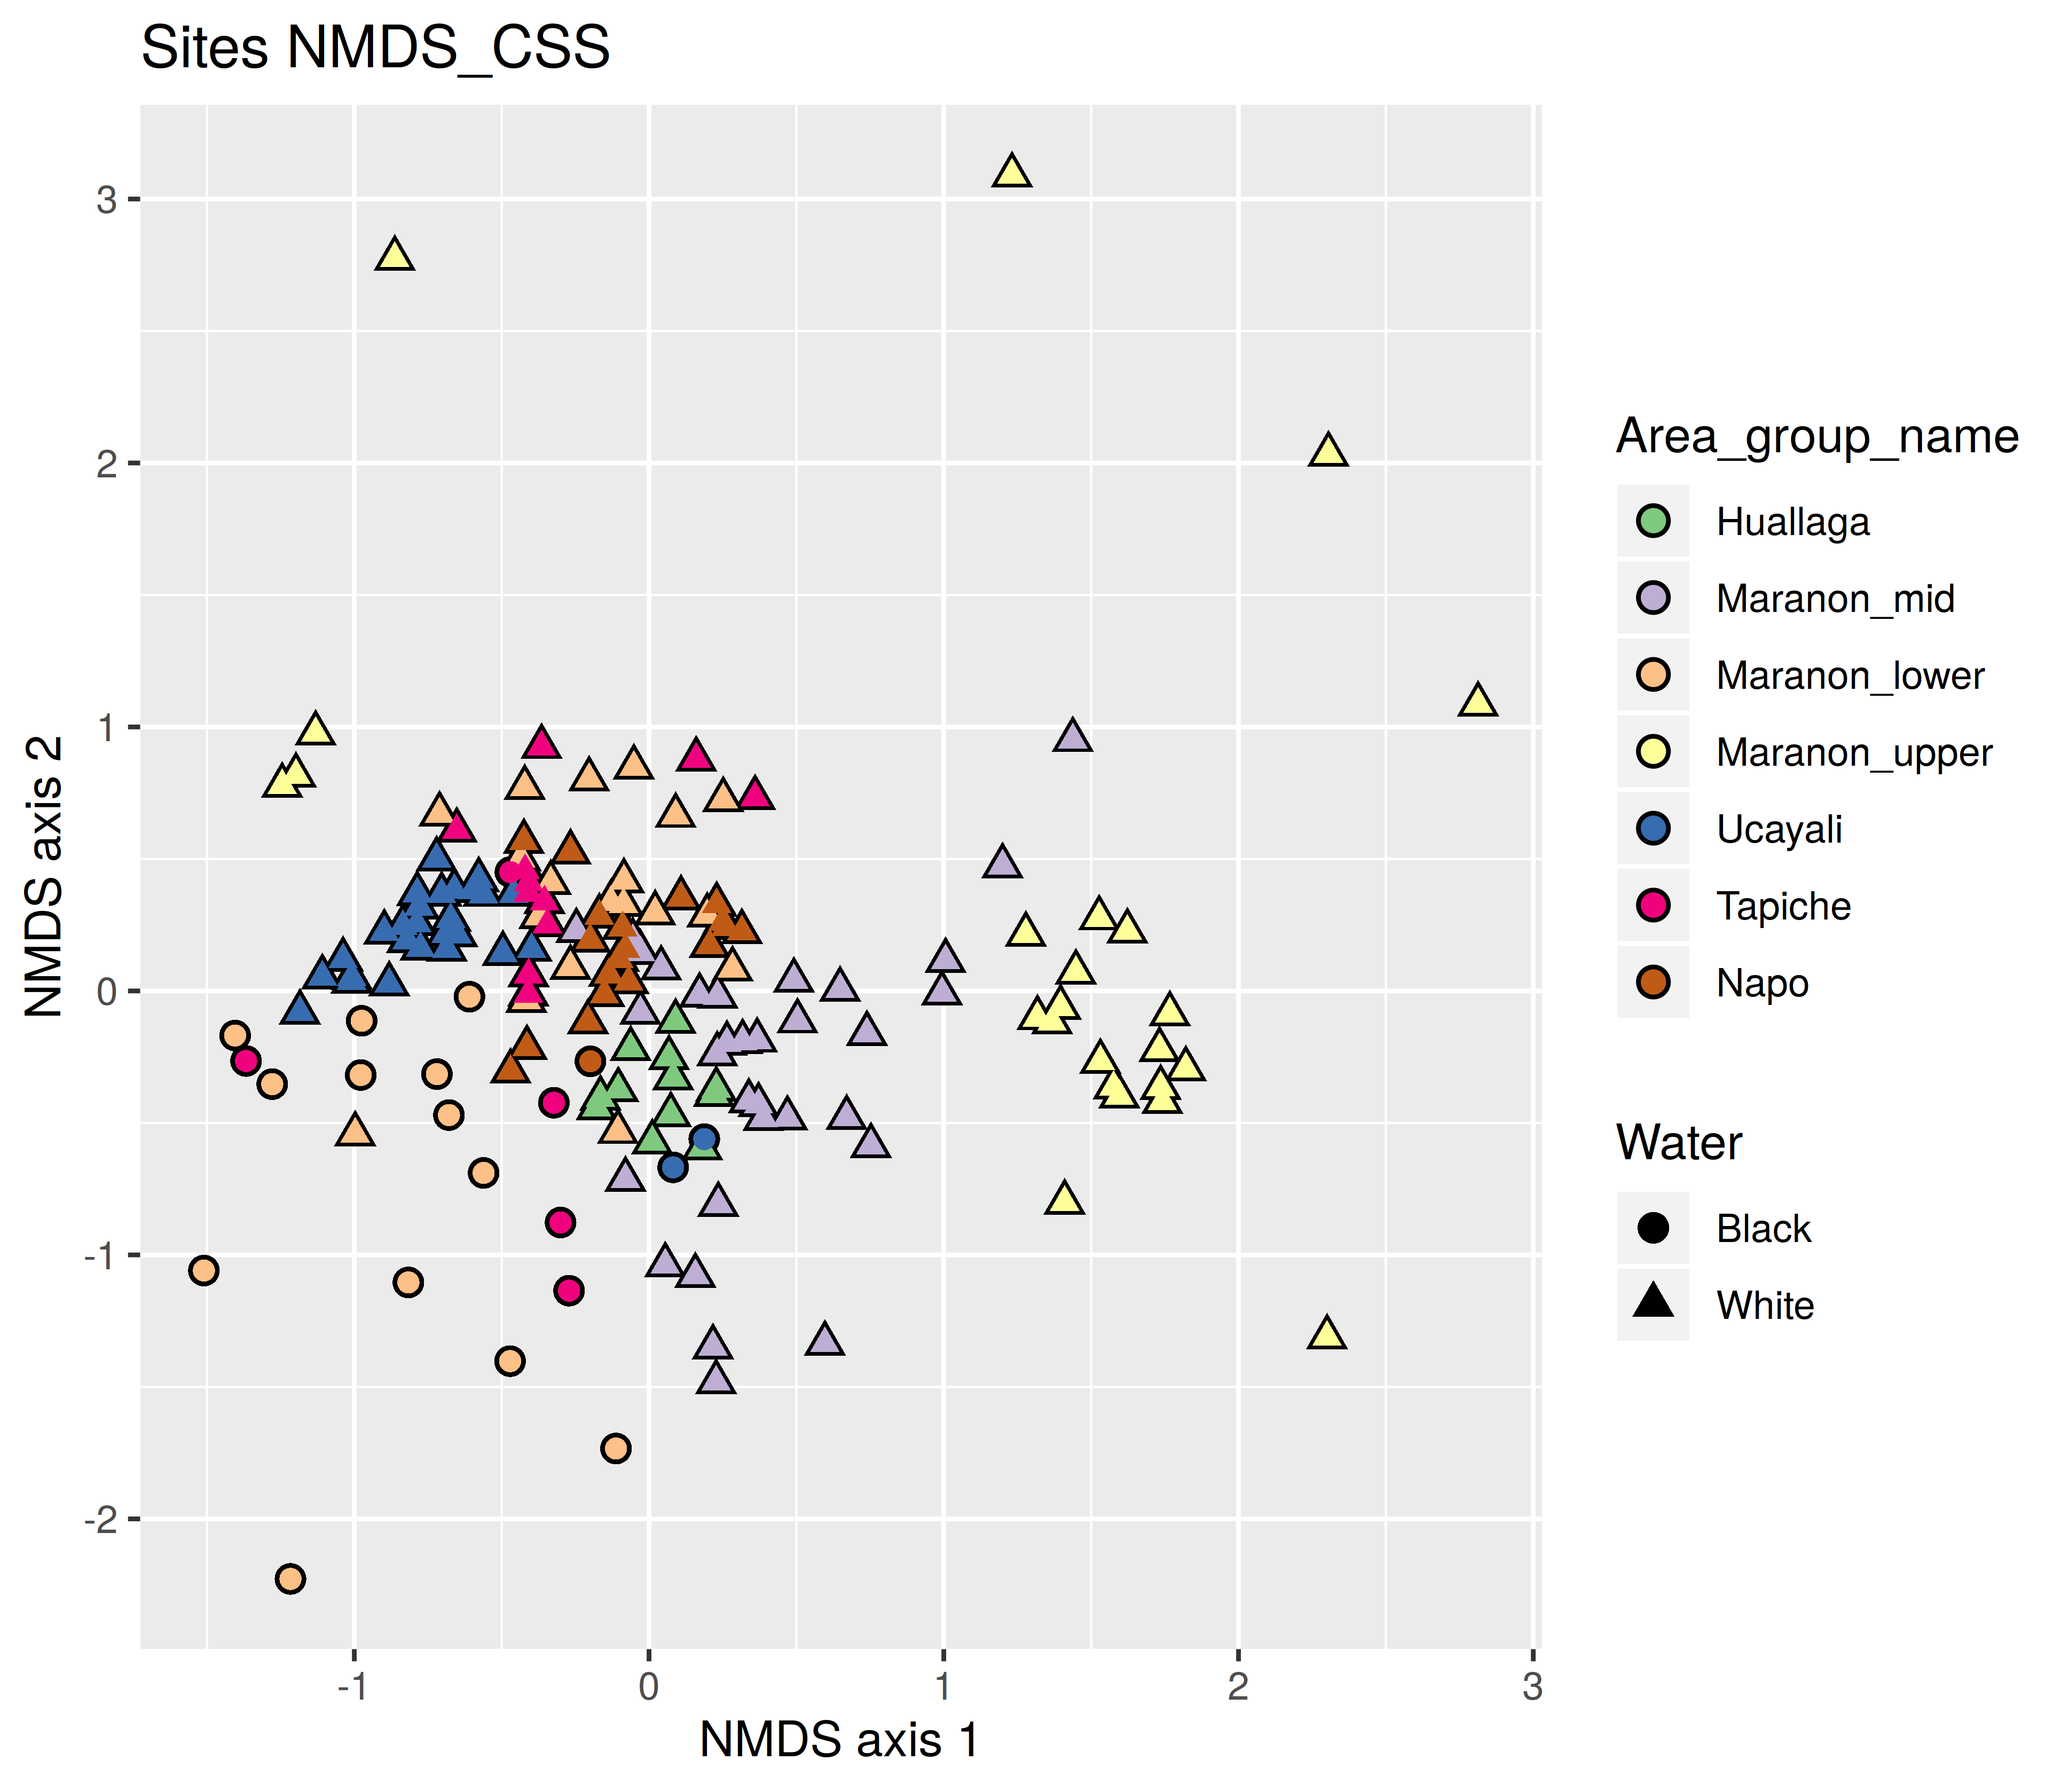
\includegraphics[width = \textwidth]{nmds12otucss}
		\caption{}
		\label{fig:nmds12otucss}
	\end{subfigure}
	\begin{subfigure}{0.4\textwidth}
		\centering
		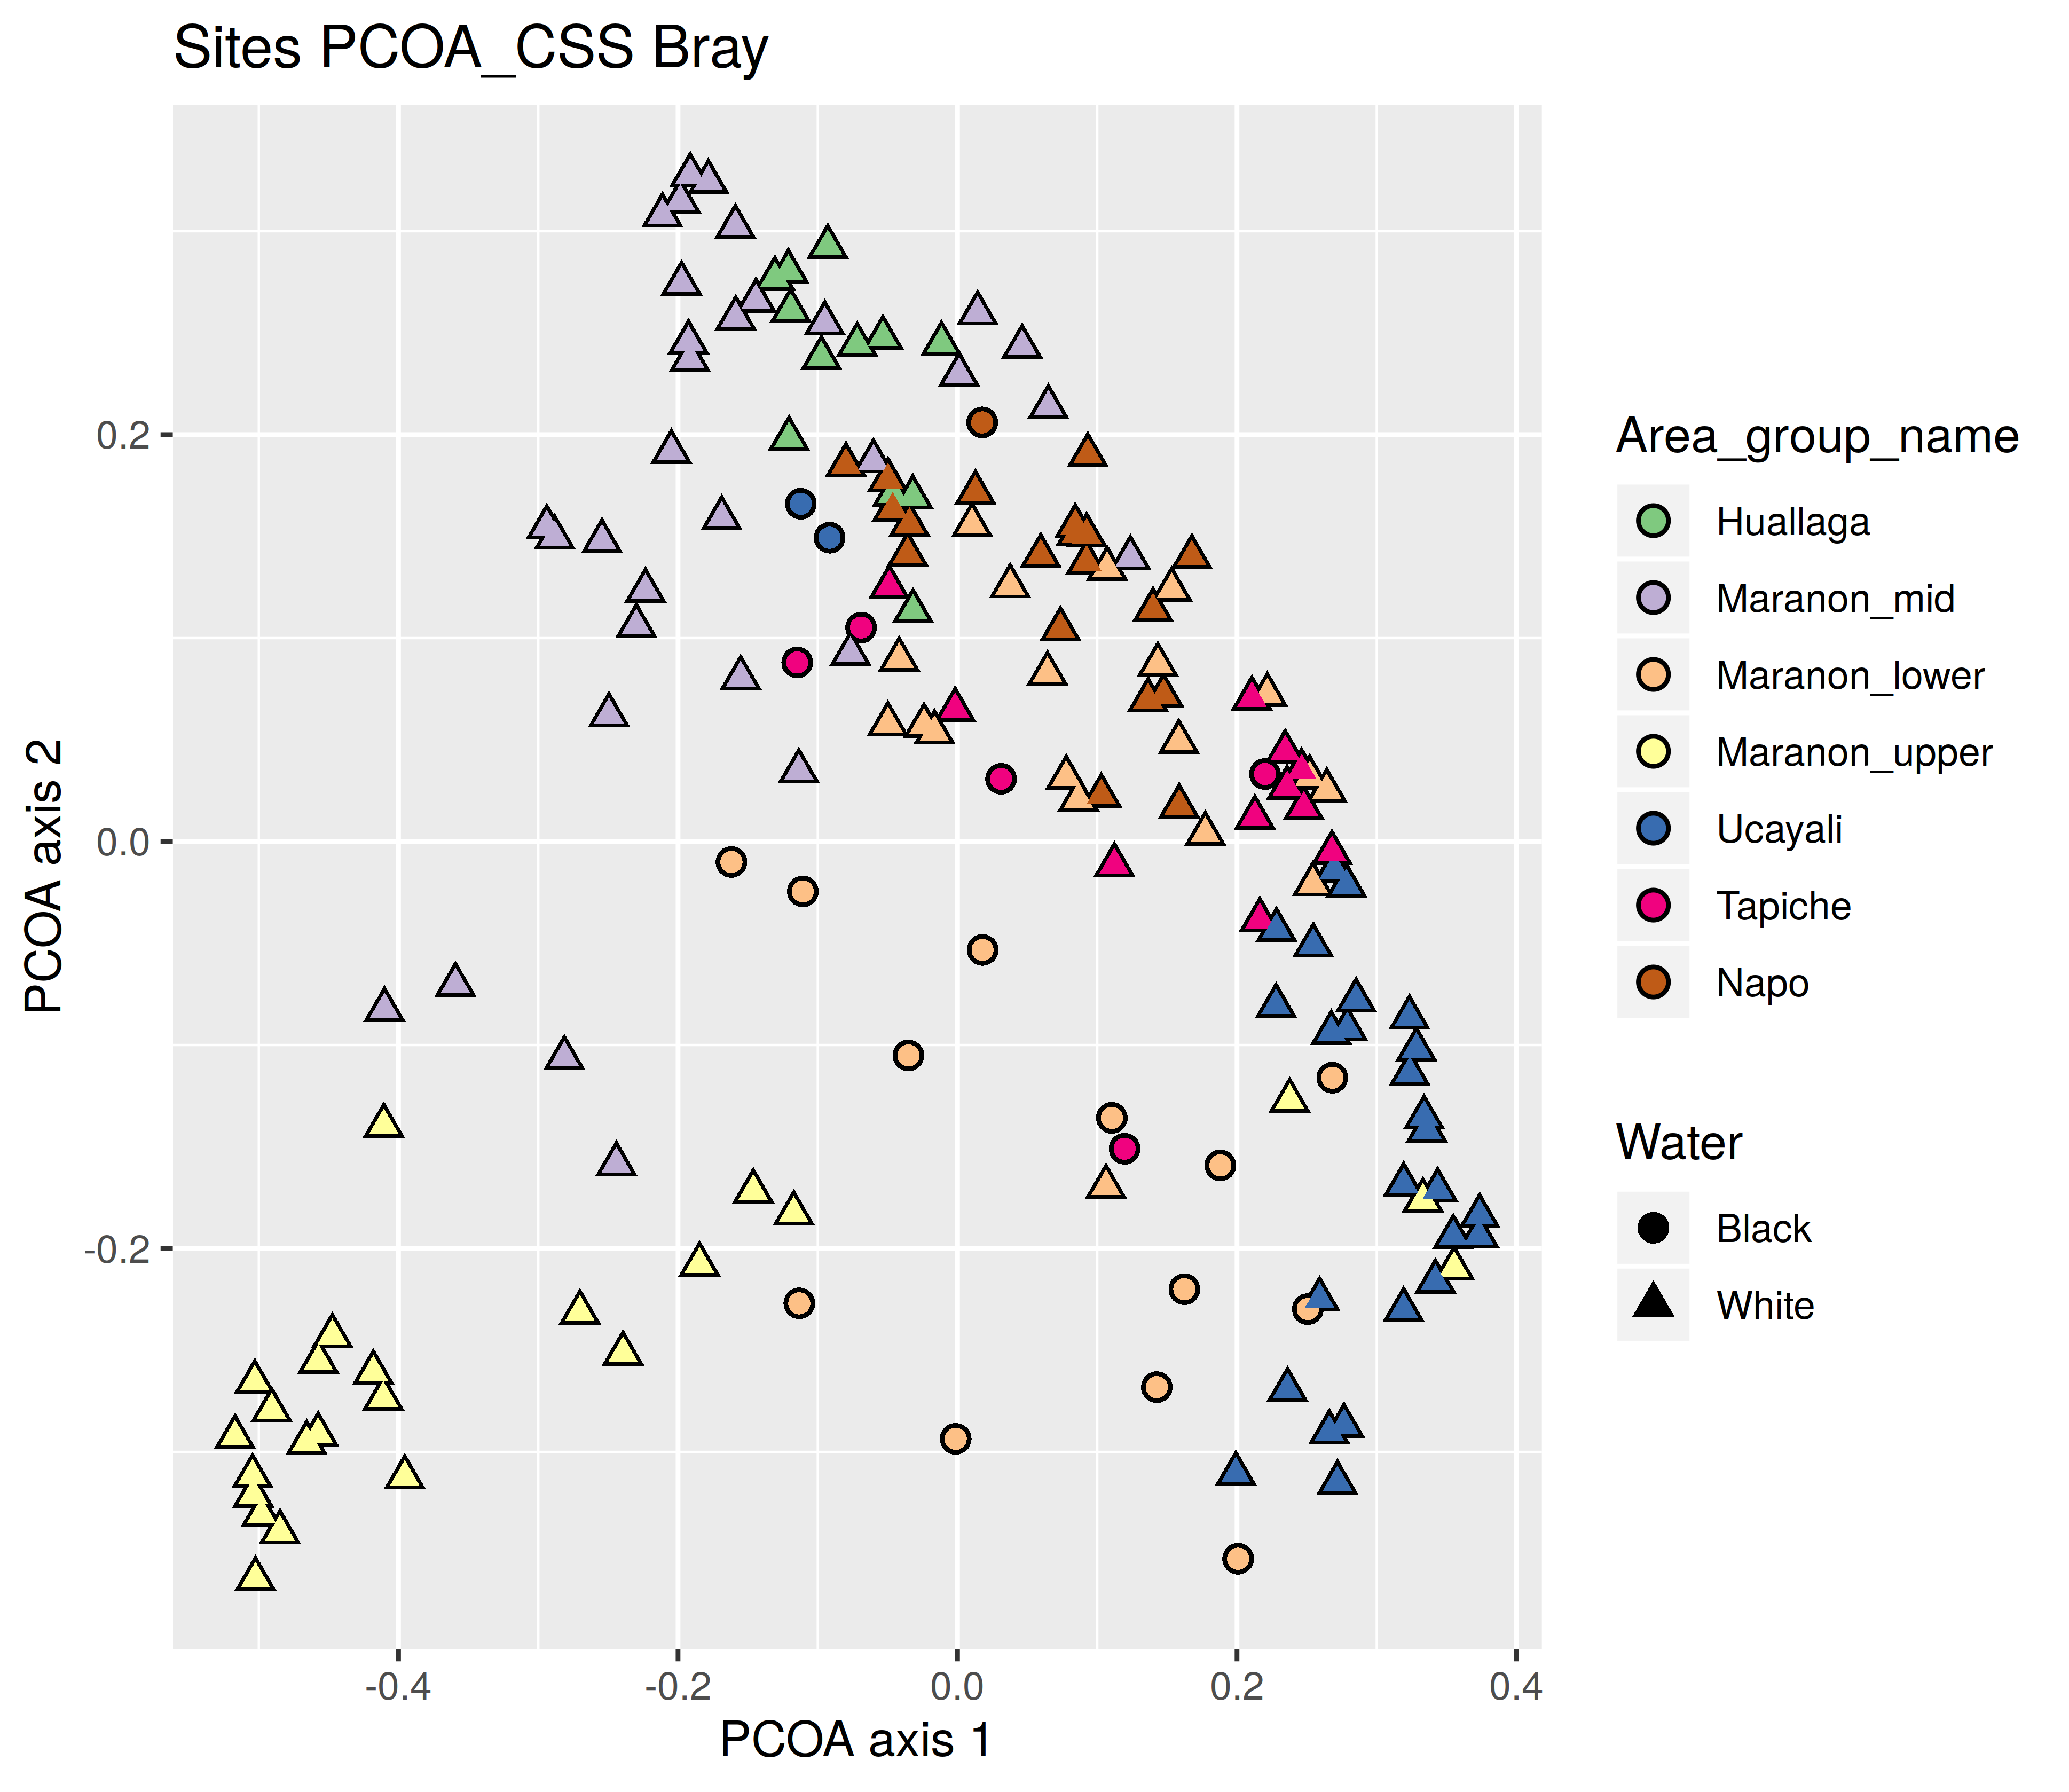
\includegraphics[width = \textwidth]{pcoa12otucss}
		\caption{}
		\label{fig:pcoa12otucss}
	\end{subfigure}
	\caption{Ordination plots for the CSS normalised data. Figure \ref{fig:nmds12otucss} shows an NMDS and Figure \ref{fig:pcoa12otucss} a PCoA plot of the data using the Bray-Curtis measure. Both methods separate white and black water samples better than when applied to non-normalised data.}
\end{figure}

We will be checking if this normalisation method and transformation produces any significant improvements (over the unnormalised dataset) in the classifiers ability to determine the river colour. 

%%Normalization, which is the process where systematic variability is identified and removed, is therefore a vital part of the data analysis. 
%https://www.ncbi.nlm.nih.gov/pmc/articles/PMC5910605/
% A substantial part of this variability is systematic and affects multiple genes and/or samples in a similar way. One example of systematic variability is the differences in sequence depth, where each sample is represented by a varying number of reads [13]. Systematic variability also comes from other technical sources, such as inconsistencies in the DNA extraction and sample handling, varying quality between sequencing runs, errors in the read mapping, and incompleteness of the reference databasescd 


\subsection{Feature Correlation}

A big minority of OTUs in our data set have been found to have an absolute Spearman correlation of more than 0.9 with at least one other OTU. This correlation has a biological underpinning as it is expected that the abundance of species in a river environment would co-vary along it's length. Relationships between species in an environment can take many forms, like parasitic (the abundance of OTU1 is increased and for OTU2 is decreased when they are both present), competitive (the abundance of both OTU1 and OTU2 is decreased when they are both present), and mutual (the abundance of both OTU1 and OTU2 is increased when they are both present). More complicated, non-linear correlation networks exist in nature between more than two species that are very difficult to capture even with large amounts of unbiased data \cite{weiss_correlation_2016}. 



For our problem at hand, recovering such correlation networks is not of interest. We are more interested in selecting the best features from our data that would aid in the classification. Thus, we used the Spearman correlation with a threshold of 0.9 to remove 122 OTUs and create a new data set without highly correlated OTUs. 










%%~~~~~~~~~~~~~~~~~~~~~~~~~~~~~~~~~~~~~~~~~~~~~~~~~~~~~~~~~~~~~~~~~
%% DATA SPLITTING
%%~~~~~~~~~~~~~~~~~~~~~~~~~~~~~~~~~~~~~~~~~~~~~~~~~~~~~~~~~~~~~~~~~
\section{Splitting}
\label{sec:splitting}

Together with the OTU table, our data also include the location of the samples in the rivers (in Easting and Northing coordinates) and in which part of the river they belong to. Because of this location attribute, our samples cannot be said to be independent. Thus, the way we choose to split our data into training and testing sets will surely affect the accuracy of the classifier. For example, testing on a set that is composed of samples maximally distant from the ones in the training set (see Figure \ref{fig:groupsamp}) will produce different results than testing on a set with all samples in close proximity to the ones in the training set (see Figure \ref{fig:stratsampl}).

To avoid choosing a split method, several ones are employed that represent different splitting conditions. The classifiers are then tested on all of them so as to evaluate how well they can perform under various circumstances.
%% Stratified an group folds for tain test split plot
\begin{figure}[h]
\centering
\begin{subfigure}{0.4\textwidth}
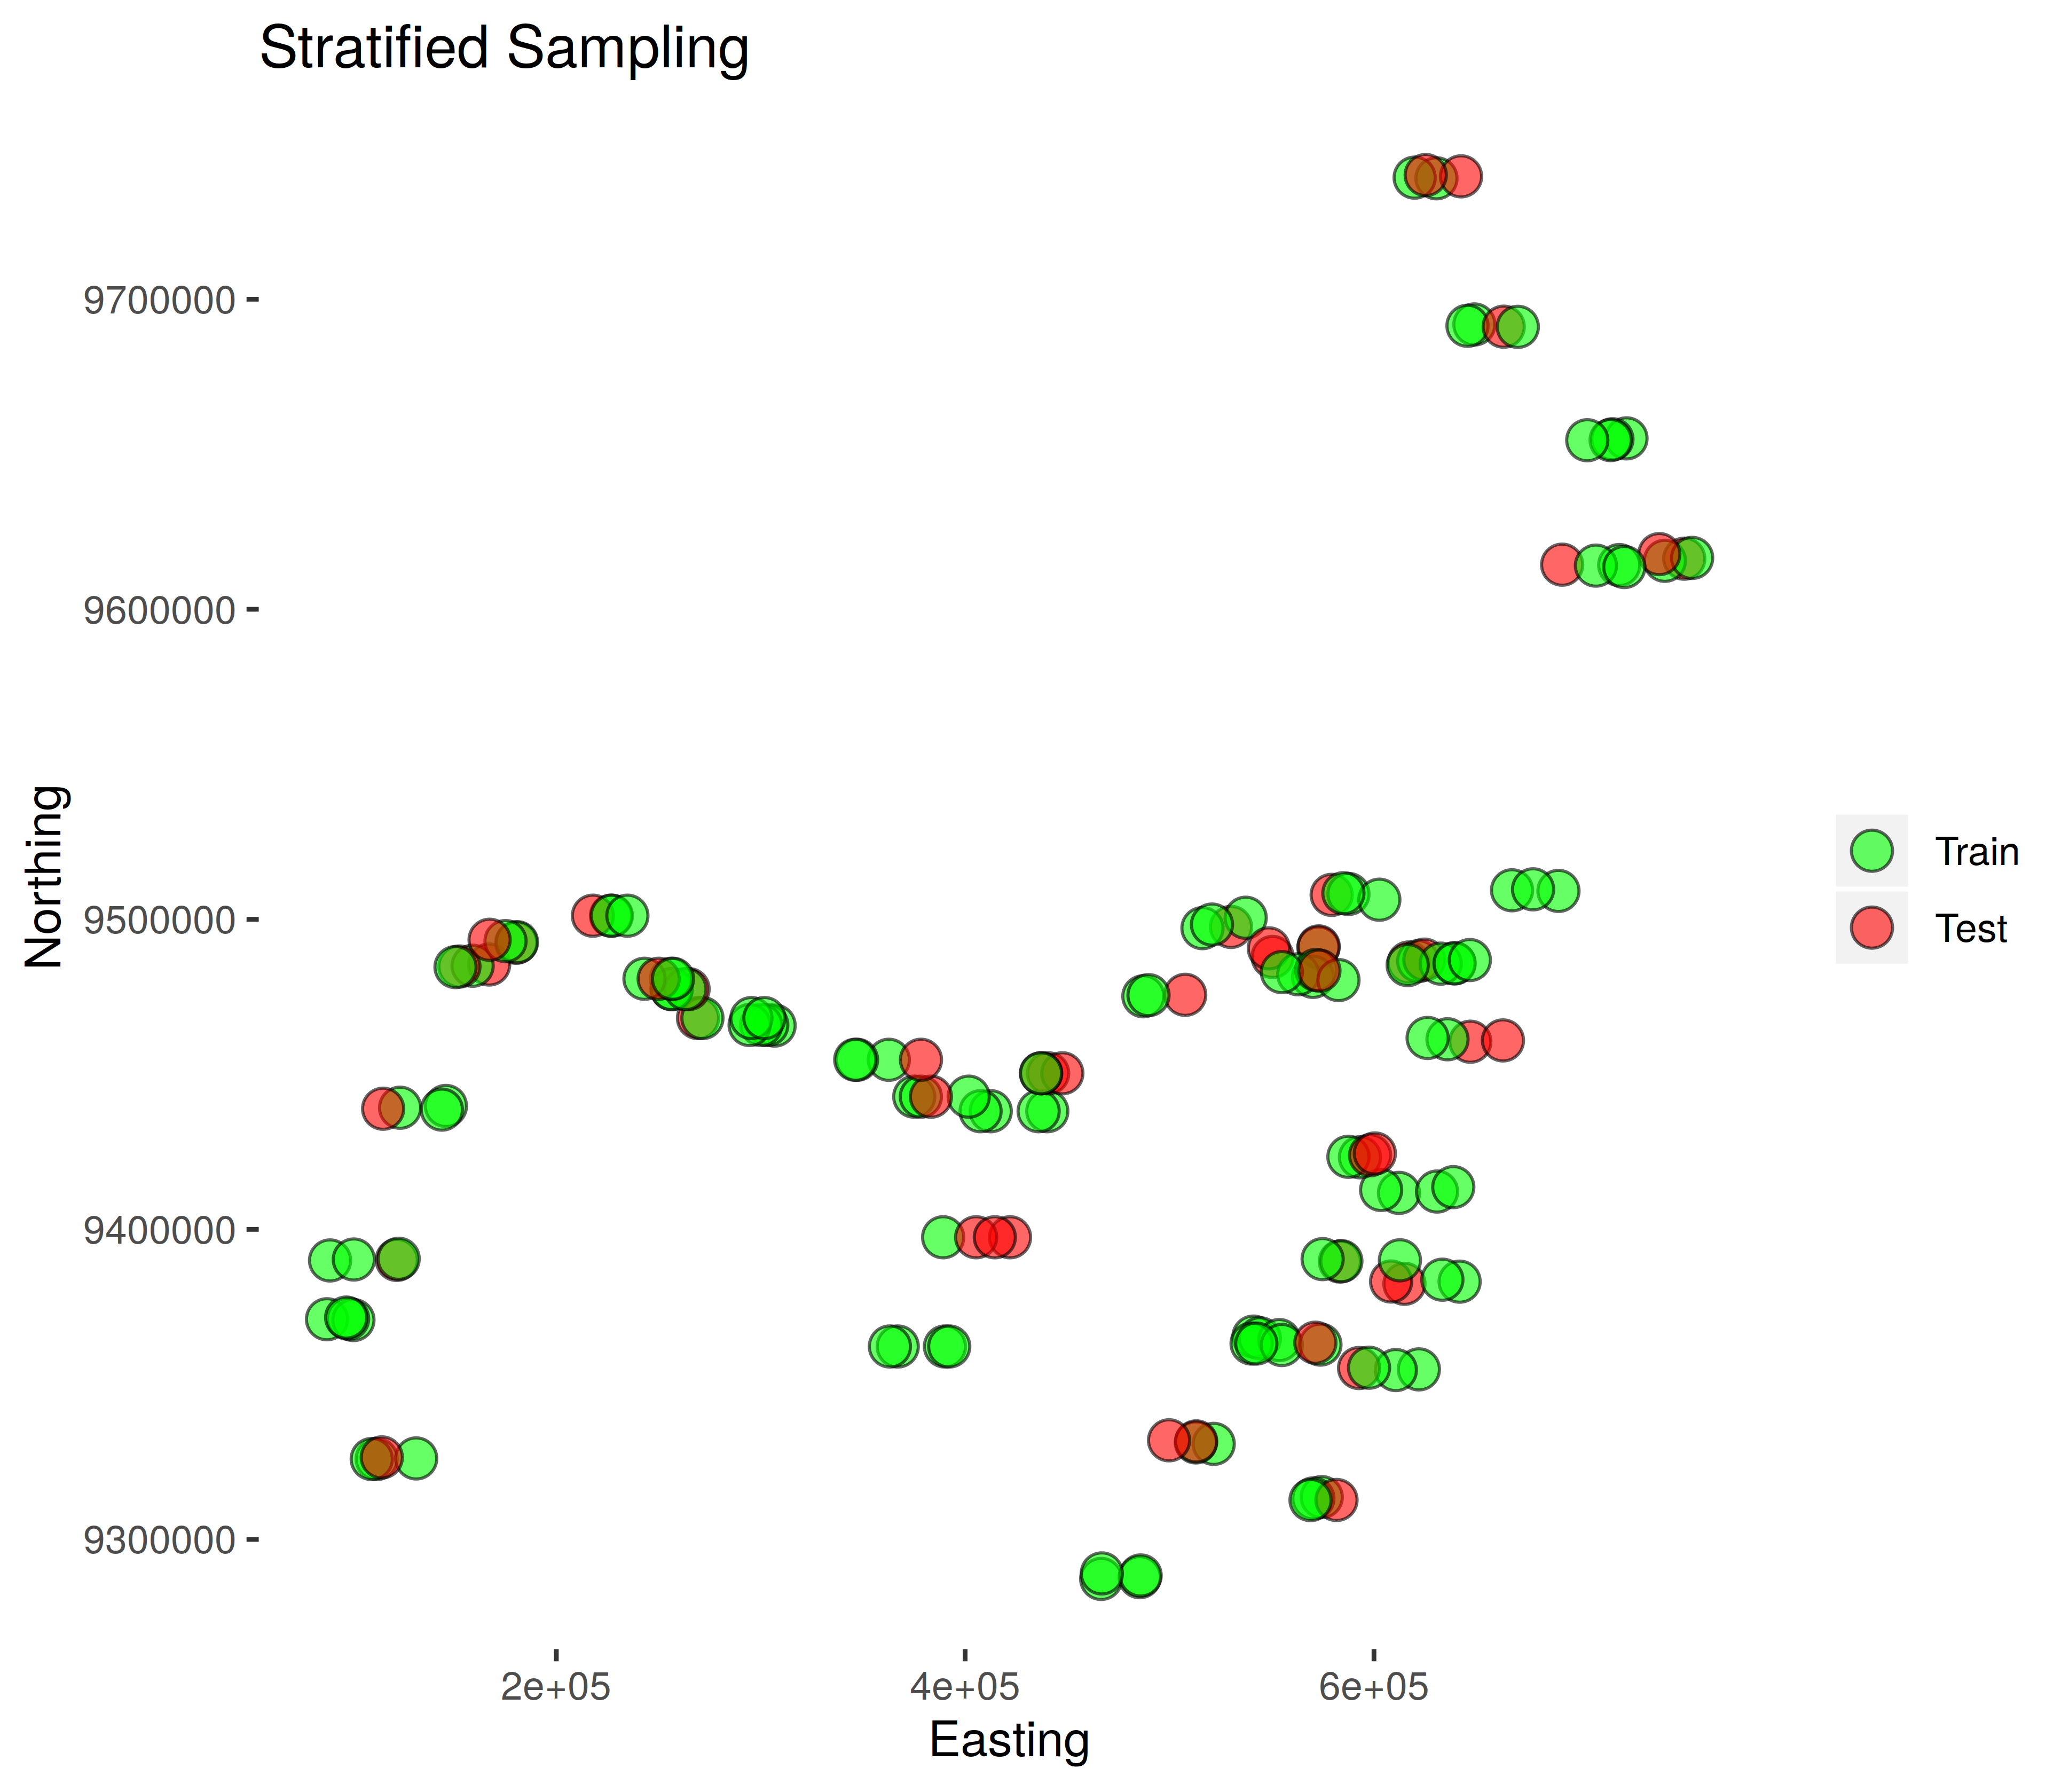
\includegraphics[width = \textwidth]{stratsamp.png}
\end{subfigure}
\begin{subfigure}{0.4\textwidth}
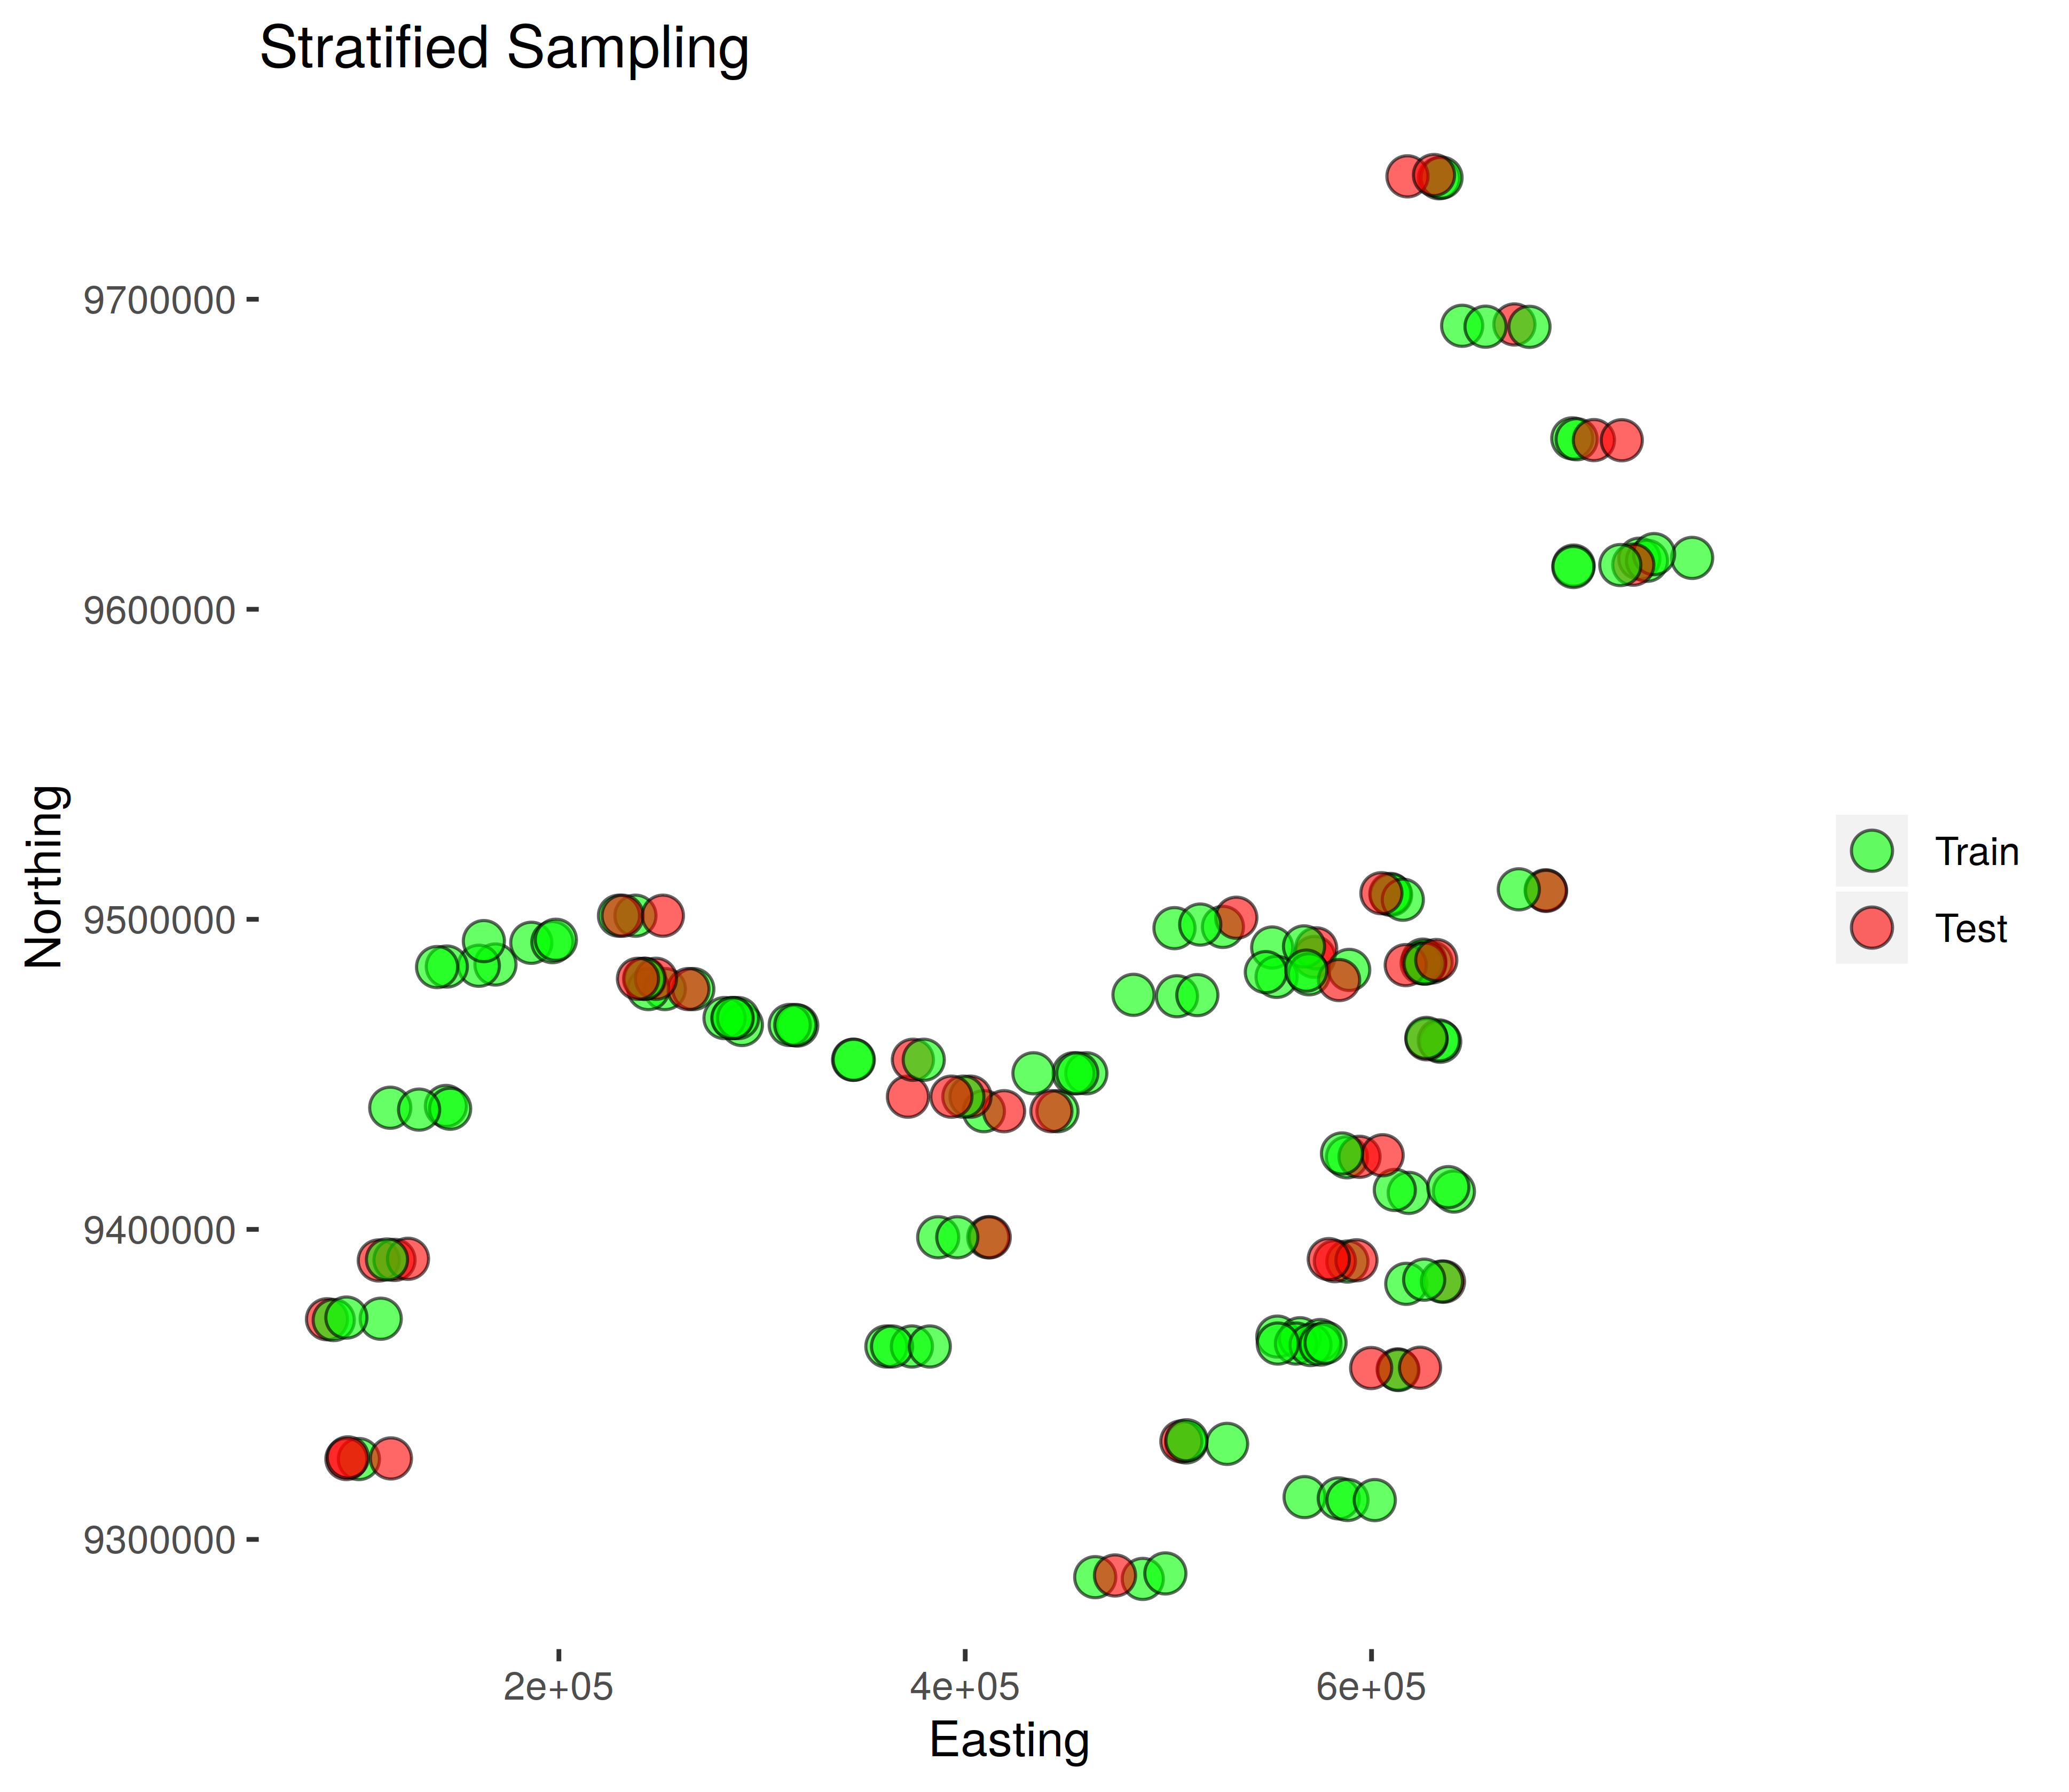
\includegraphics[width = \textwidth]{stratsamp2.png}
\end{subfigure}
\caption{Test set samples are selected such that they are located among the Train set. This represents a maximally similar split which is created by ensuring constant distribution of samples in each part of the river in both the Train and Test set.}
\label{fig:stratsampl}
\end{figure}

%Group sample plot
\begin{figure}[h]
\centering
\begin{subfigure}{0.4\textwidth}
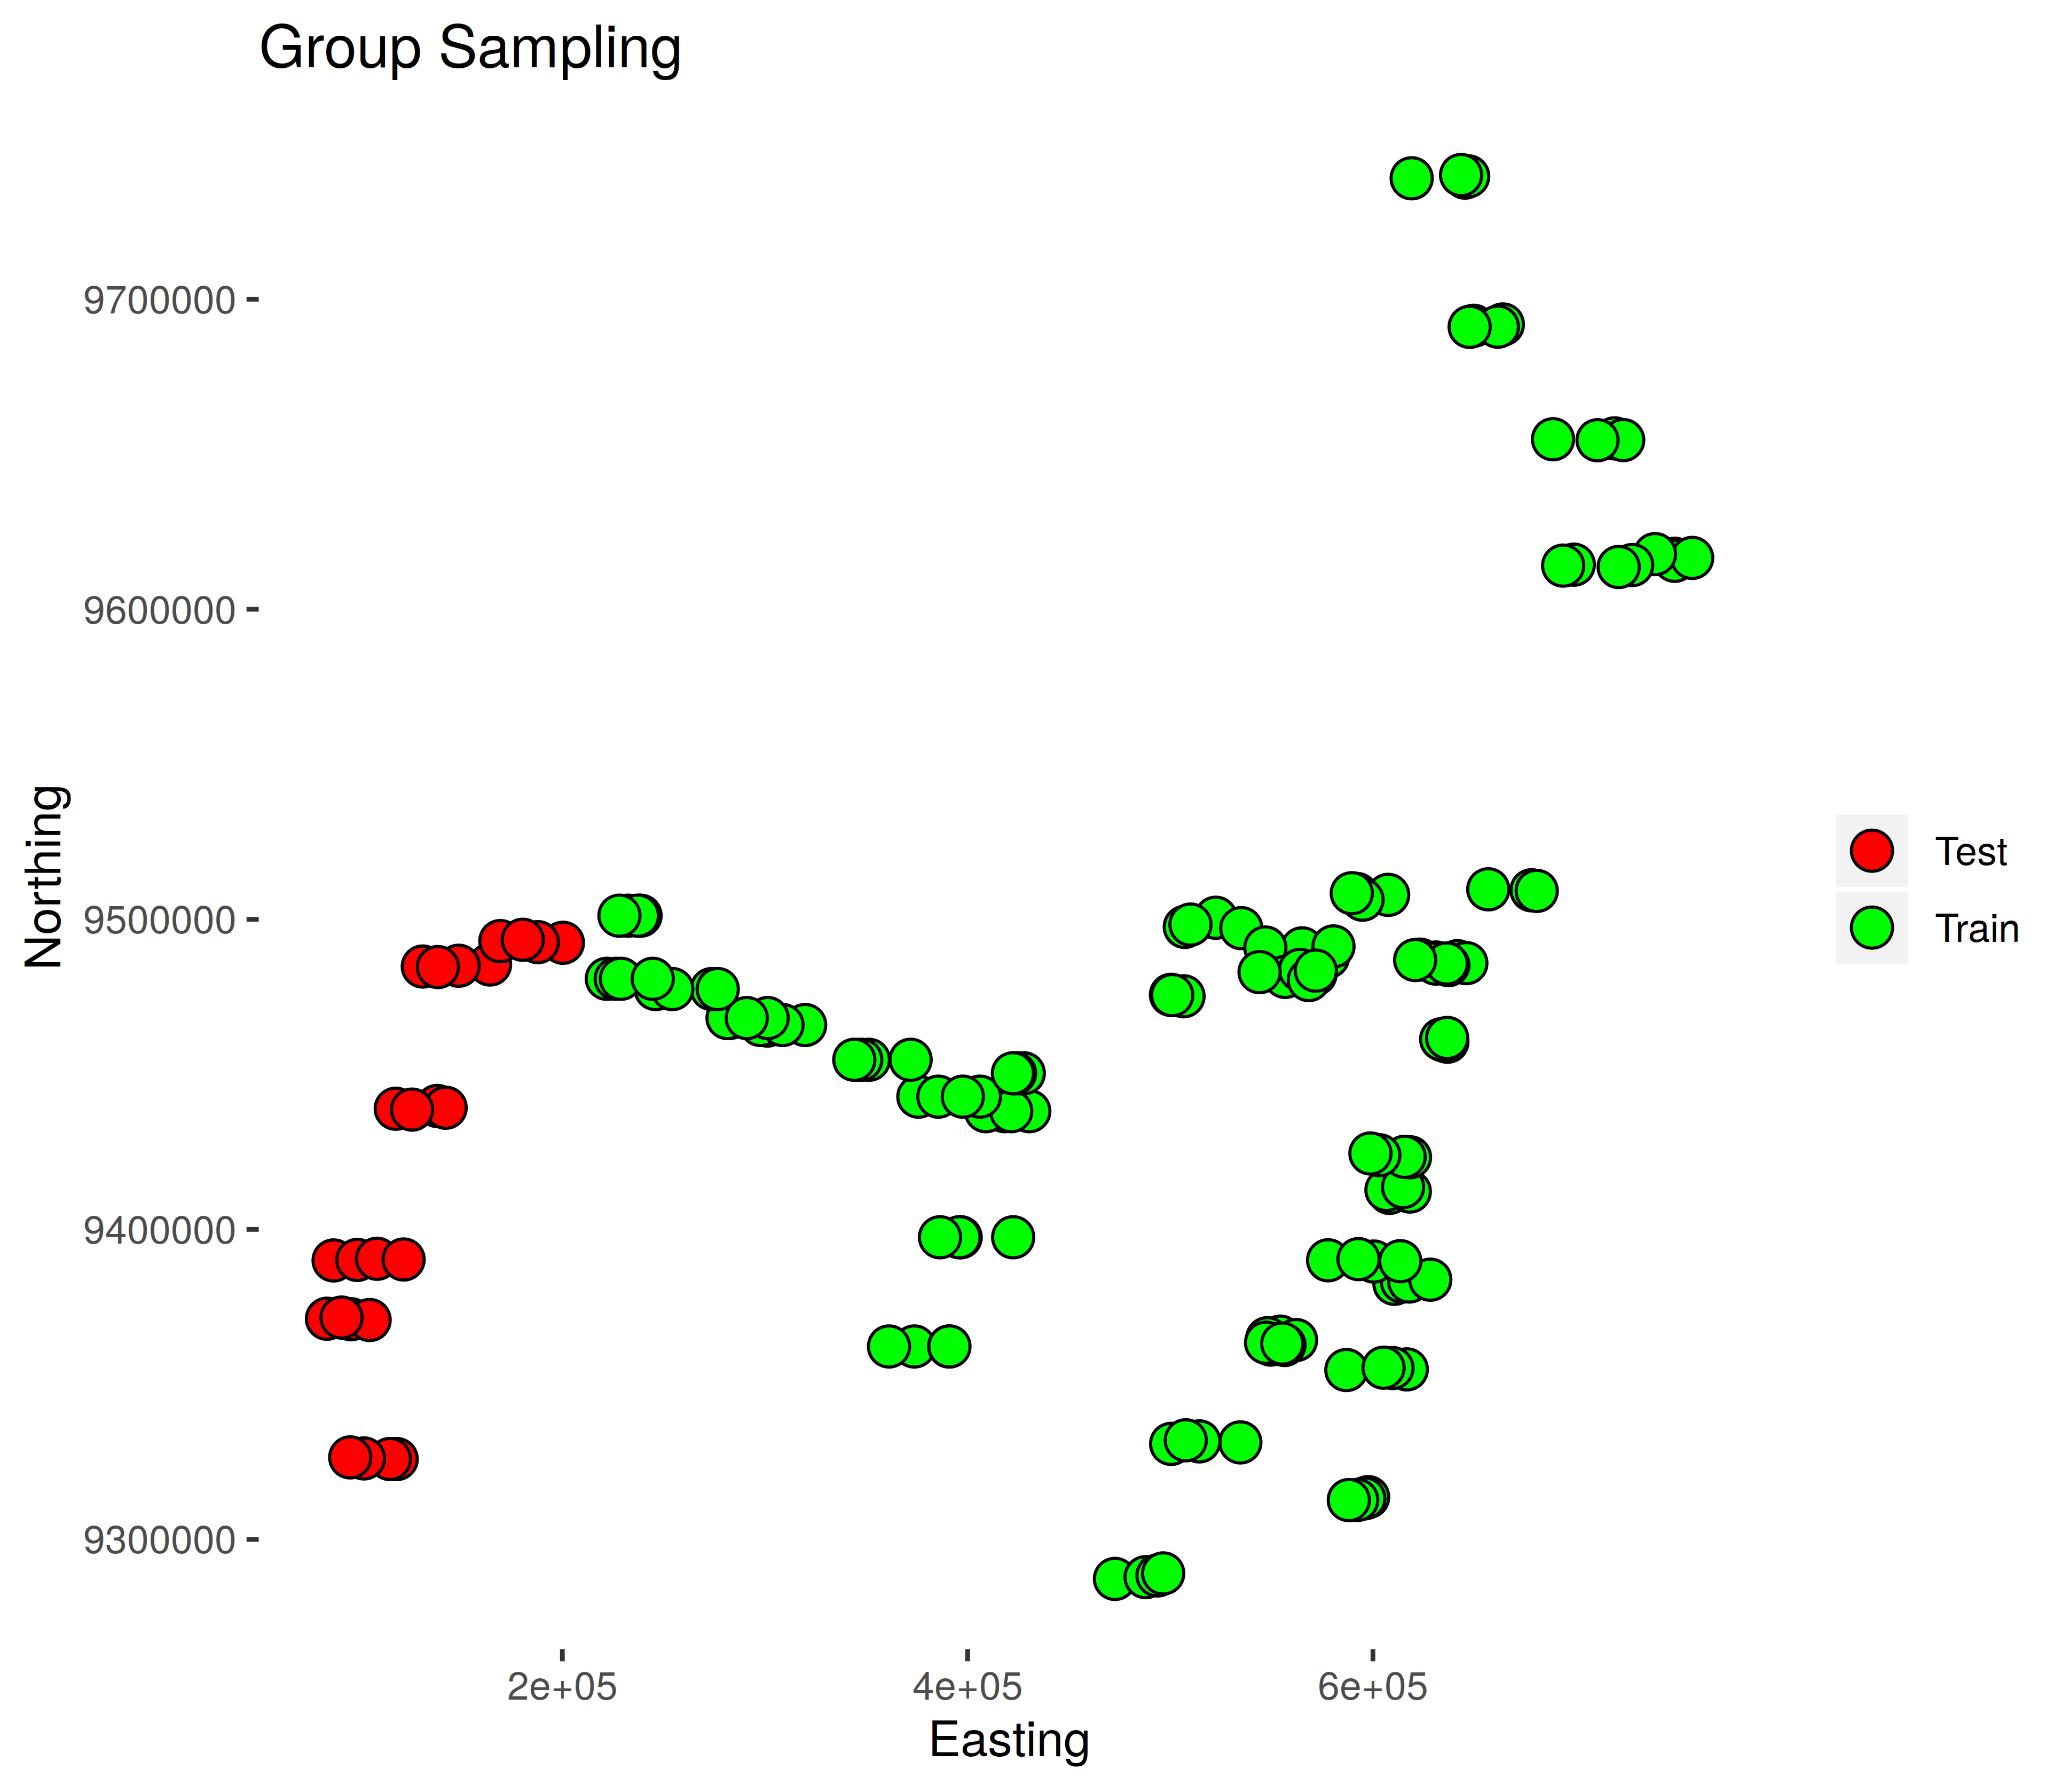
\includegraphics[width = \textwidth]{groupsamp.png}
\end{subfigure}
\begin{subfigure}{0.4\textwidth}
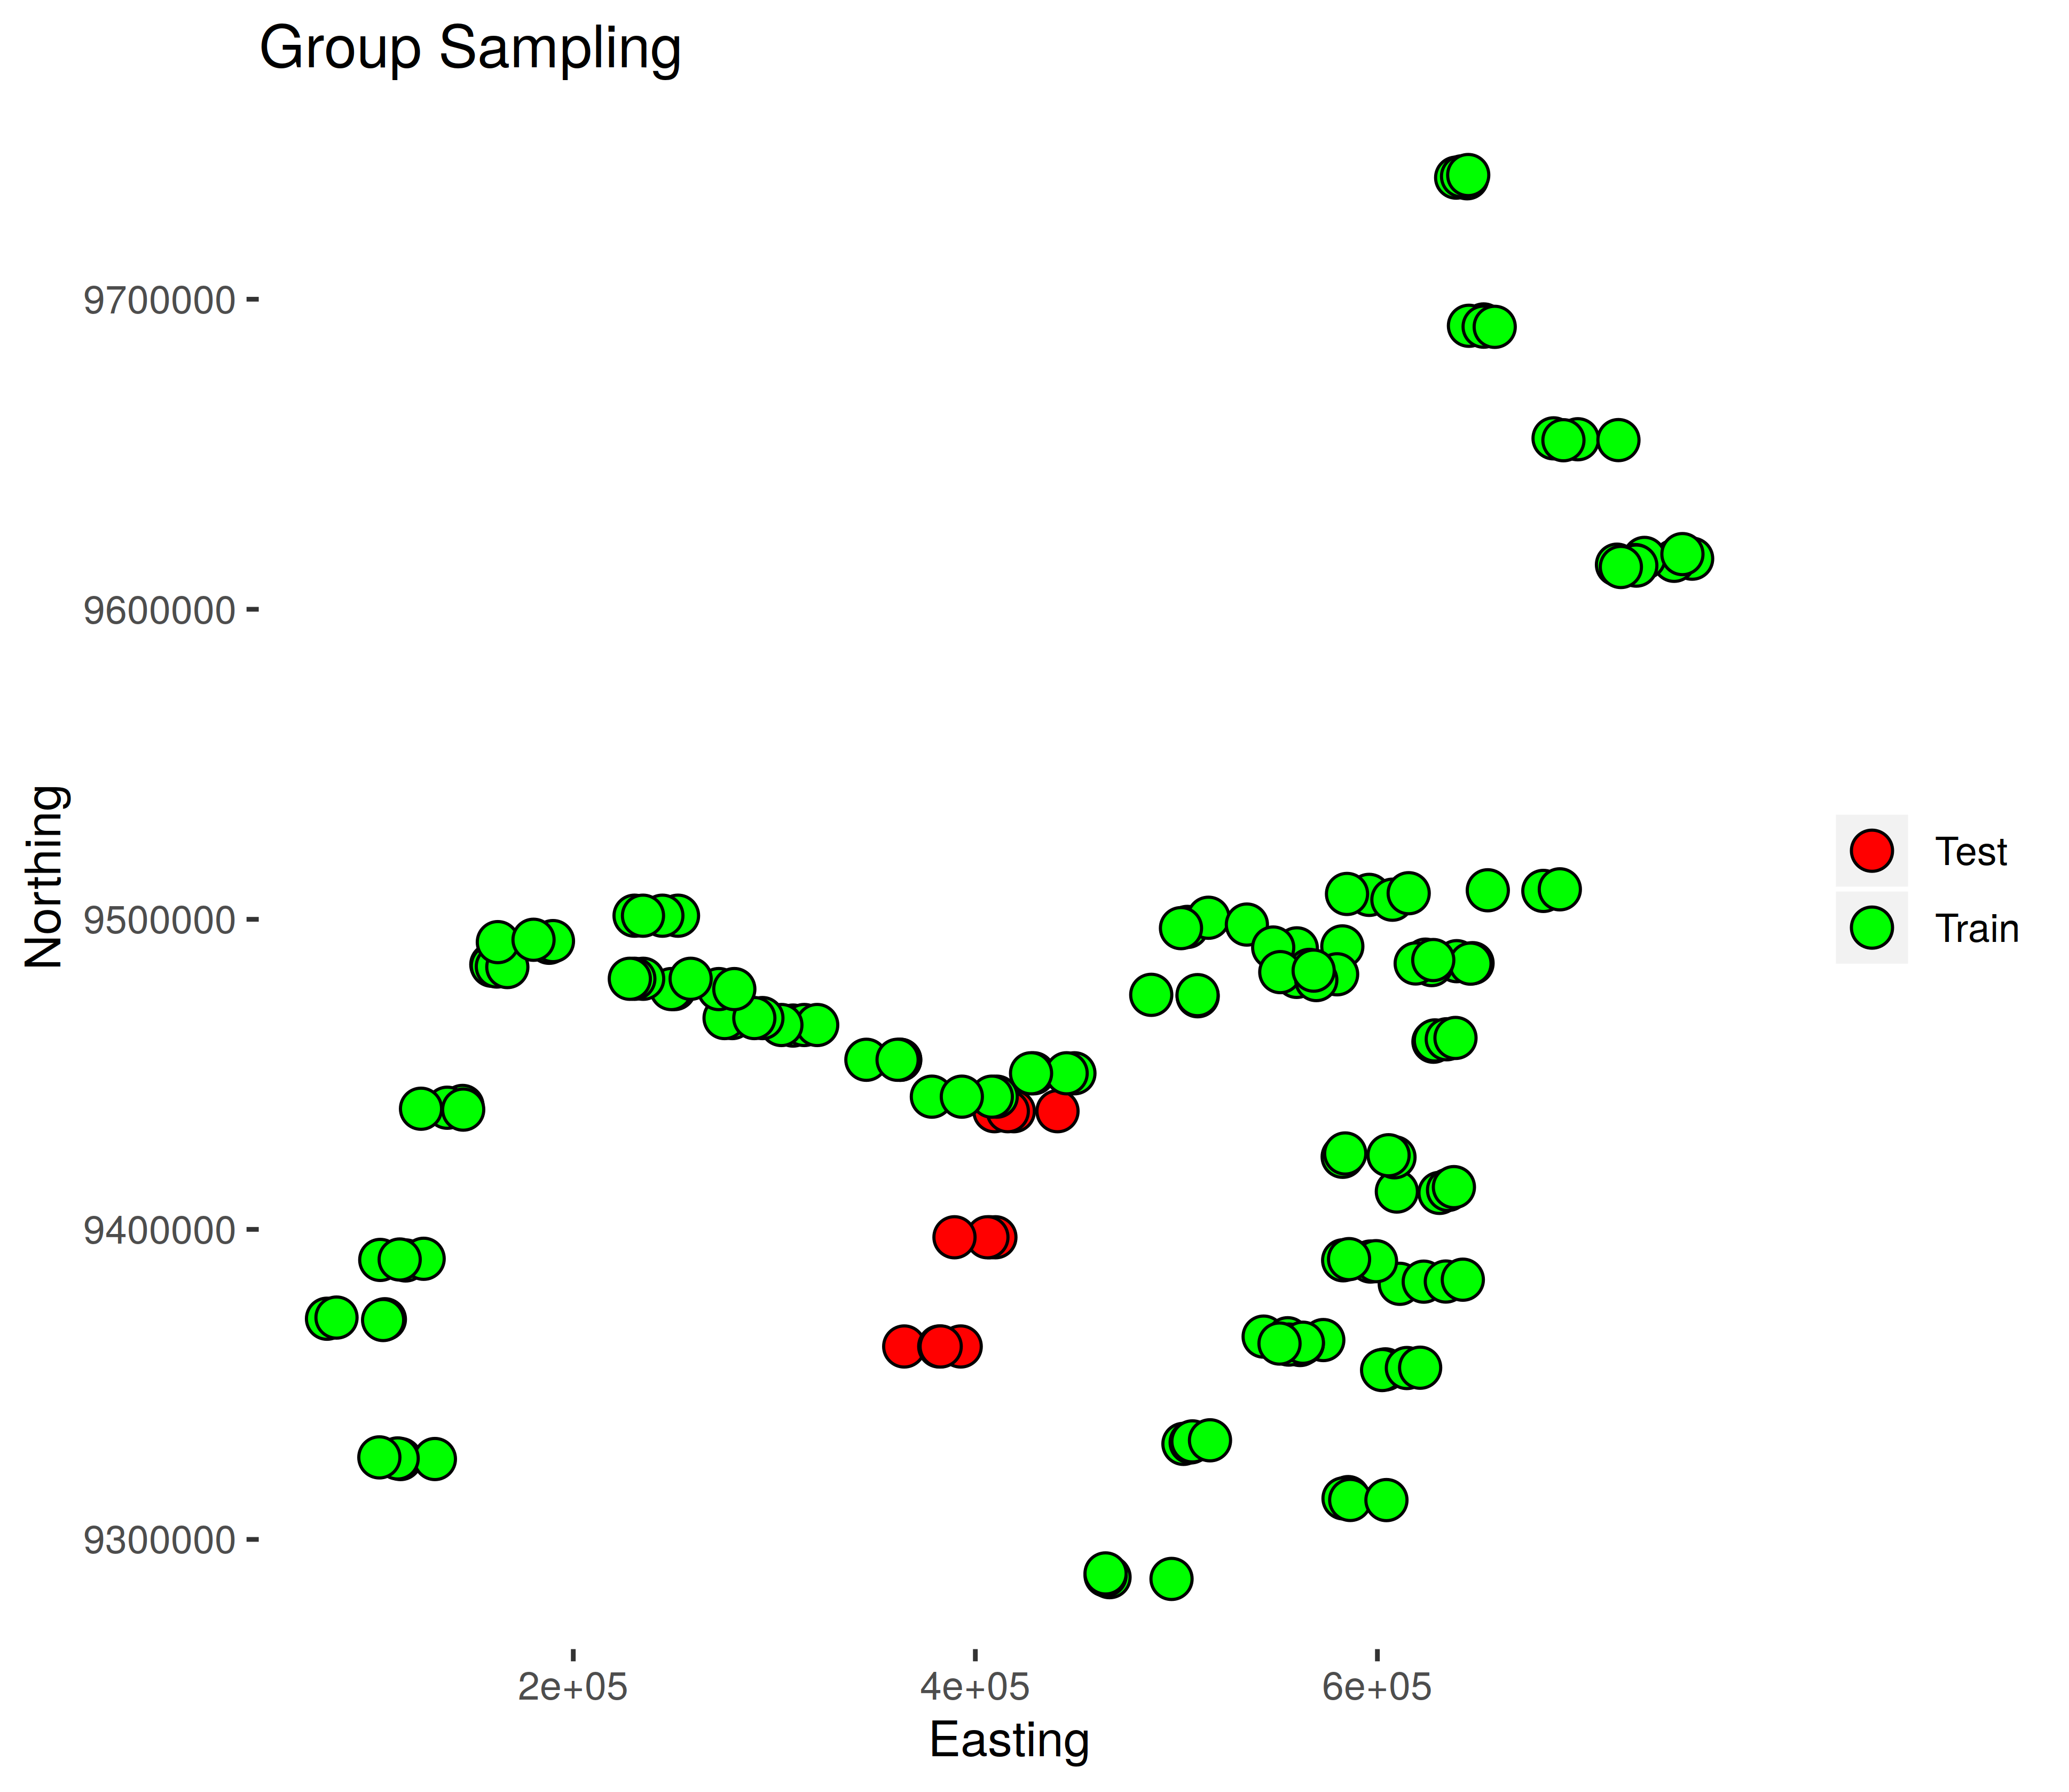
\includegraphics[width = \textwidth]{groupsamp2.png}
\end{subfigure}
\caption{Test set samples are geographically distinct from Train set samples. This represents a maximally dissimilar split which is created by choosing a different part of the river as the Testing set.}
\label{fig:groupsamp}
\end{figure}




%Validation sets
In addition to splitting the data into training and test sets, the train set is further split into validation sets so as to tune the hyperparameters of the models. The splitting into validation sets follows the same principle/method as the train-test split. So if, for example, the train and test sets are split using the maximally similar approach, the validation sets created from the train set are chosen so as to be maximally similar to the remaining set.


The steps of testing a classifier using a specific split method are as follows:
\begin{enumerate}
\item A set of hyperparameters values are chosen for the cross-validation procedure. For example, in Logistic Regression a set of numbers ranging from 0.001 to 20 is chosen for the sparsity parameter and the set $\{True,False\}$ is chosen for the intercept parameter.
\item The data set is split into train and test sets based on the splitting method of choice. 
\item The train set is split into $K$-folds, each being a validation set, using the same method as for the train-test split. 
\item The classifier is trained on the $K-1$ folds and tested on the remaining validation set for all possible combinations of hyperparameters (e.g. the Logistic Regressor is trained with hyperparameters $\{0.001,True\},\{0.001,False\},\{1.001,True\},\{1.001,False\}$ etc...).
\item Step 4 is repeated for all the $K$-folds (by training on the $K-1$ and testing on the one left out). The average score across the validation sets is found for each hyperparameter combination and the classifier is retrained on the train set using the best hyperparameters set.
\item The retrained model is tested on the test set and the confusion matrix is calculated.
\item Steps  2 through 6 are repeated a number of times for different train-test splits using the same split principles. The confusion matrix for each repetition is stored and added at the end of the process.  
\end{enumerate}

 
The best hyperparameters are the ones that maximise either the F score or accuracy. The former combines both the precision and recall of the validation test. Precision is the number of correctly identified positive results divided by the number of all positive results returned by the classifier. Recall is the number of correctly identified positive results divided by the true number of positive results. The score is the harmonic mean of the two
\begin{equation}
	F_1 = \frac{2}{\text{recall}^{-1} + \text{precision}^{-1}}.
\end{equation} 
Choosing black water as the positive result would lead to cases were recall is undefined; in the case of maximum dissimilarity, a validation set might end up with only white water samples (thus only negatives). So recall, which measures how many positive observations were correctly identified from the total number of positive observations, would be $\frac{0}{0}$. Thus, white samples are chosen as the positive observations.

The whole testing procedure is repeated using accuracy as the metric for picking the best hyperparameters. This is because the F score might lead to choosing classifiers that minimise False Negatives (maximising recall), and as such, have an increased concentration of mistakes in identifying black water samples.

This procedure can be repeated for different features (data sets), so as to evaluate how feature selection and transformations can alter the results.
% The best classifier for the particular features and splitting method is the one which has the highest mean score across all train-test splits. 
 The various data sets used to test the classifiers on are summarised in table \ref{table:features}.
\begin{table}
	\caption{Features used in Classification}
	\centering
	\label{table:features}
	\begin{tabularx}{\textwidth}{l X  }
		\hline 
		Features used &Description of dataset\\ 
		
		\hline
		OTU &The OTU table as it is \\
		OTU LOW & The OTU table without highly correlated features\\
		OTU CSS & The CSS normalised OTU table\\
		OTU Min CSS & The CSS normalised OTU table without samples with total read counts of less than 10000 reads  \\
		OTU CSS LOG & A $\log_2$ transformed OTU CSS \\
		PCoA Bray-Curtis &The transformation of the OTU table with PCoA using the Bray-Curtis measure  \\
		PCoA Bray-Curtis CSS &The transformation of the OTU CSS table with PCoA using the Bray-Curtis measure\\
		
		\hline 
	\end{tabularx}
\end{table}


A baseline benchmark for this problem is also set so that the classifiers' evaluation is meaningful. We are essentially setting the `coin flip'/naive rate; prediction based on prior probabilities of the classes. Using their distribution on the whole data set (87.2\% of samples come from white water) would be an unfair baseline for the classifiers since they are trained only on a fraction of it, and the proportions of black and white water samples change significantly with the train set. 

Thus, for every train-test split we calculate the prior probability $P(C=1)$ of a sample being white, using the train set, by dividing the number of white samples by the total number of samples. Then, for each observation in the test set $y_i \in \{1 for White, 0 for Black\}$ we calculate the expected times the `coin' would identify it correctly and falsely
\begin{align}
	E(\text{Correct Prediction}|y_i ) = y_i*P(C=1) + (1-y_i)*(1-P(C=1)) \\
	E(\text{False Prediction}|y_i) = (1-y_i)*P(C=1) + y_i*(1-P(C=1)).
\end{align}
A confusion matrix is constructed (see table \ref{table:baseline}) using the total number of white $N_{white}$ and black $N_{black}$ water samples in the test set.
\begin{table}[h]

	\centering

	\begin{tabularx}{\textwidth}{l| c c}
	 
		 &Predicted Black&Predicted White\\ 
		
		\hline
		Actual Black&$N_{black}*E(\text{Correct}|\text{Black} )$&$N_{black}*E(\text{False}|\text{Black})$\\
		Actual White& $N_{white}*E(\text{False}|\text{White} )$&$N_{white}*E(\text{Correct}|\text{White})$

	\end{tabularx}
	\caption{Confusion matrix of baseline benchmark}
		\label{table:baseline}
\end{table}

{ \large\bf Maximising Similarity} \\
\textit{Aim}: Evaluate how well the classifiers perform when they are tested on a set which is similar geographically to the train set.\\
\textit{Method}: Testing and validation sets are made up of samples coming from every part of the river. Care is taken to ensure that no geographical area is over represented. This is done using Stratified sampling (using the method StratifieKfold) where the strata (or groups) are the areas of the rivers the samples belong to. Stratified sampling ensures that the distribution of test or validation samples in each area is approximately the same as for train samples.




{ \large \bf Maximising Dissimilarity}\\
\textit{Aim}: Evaluate how well the classifiers perform when they are tested on a set which is dissimilar (or far away) geographically to the train set.\\
\textit{Method}: Testing and Validation sets are made up of all the samples which belong to a particular area of the river. For example, the test set might be constituted by all the samples in the Upper Maranon area, and the validation sets by all the remaining areas (Huallaga, Min Maranon, Lower Maranon, Ucayali, Tapiche, and Napo). The method we use to produce these splits is GroupKfold.

{\large \bf Random Splits}\newline
\textit{Aim}: Evaluate the performance of the classifiers on train and test sets obtained by random splitting \\
\textit{Method}: Test and Validation sets are obtained by randomly splitting the data. Care is taken to ensure that the balance of white and black water samples is the same across splits. This is done using Stratified sampling with the colour of the river as the strata.


{ \bf Ideal Splits}
An ideal sampling method would take into account the spatial correlation structures between the samples, besides just their location. Since the river flows eastwards from Maranon Upper down to all other streams, samples collected upstream would inevitably affect those from downstream, but the opposite might not be true. Thus, euclidean proximity of the river samples is not always a good enough indicator for detecting similarity between samples. For example, sample A collected near the opening of the Tapiche stream and sample B collected a bit further South of the opening, in the Ucayali stream, will have a smaller distance between them than with other samples collected further south in the Tapiche and Ucayaly streams. However, since the streams diverge, A and B might be more similar to samples found downstream their part of the river (Tapiche and Ucayaly respectively) than between them. 

To achieve this, a directed graph of the river can be constructed, with vertices representing the samples, and edges the river path between them. Then a sampling scheme can take into account the stream direction and split the dataset in more sophisticated ways. One such way can test a classifier's ability to predict river colour if the test set is downstream from the train set, and the opposite, if the test set is upstream from the train. 


%\begin{table}
%\caption{Even better looking table using booktabs}
%\centering
%\label{table:good_table}
%\begin{tabular}{l c c c c}
%\toprule
%\multirow{2}{*}{Dental measurement} & \multicolumn{2}{c}{Species I} & \multicolumn{2}{c}{Species II} \\ 
%\cmidrule{2-5}
%  & mean & SD  & mean & SD  \\ 
%\midrule
%I1MD & 6.23 & 0.91 & 5.2  & 0.7  \\
%
%I1LL & 7.48 & 0.56 & 8.7  & 0.71 \\
%
%I2MD & 3.99 & 0.63 & 4.22 & 0.54 \\
%
%I2LL & 6.81 & 0.02 & 6.66 & 0.01 \\
%
%CMD & 13.47 & 0.09 & 10.55 & 0.05 \\
%
%CBL & 11.88 & 0.05 & 13.11 & 0.04\\ 
%\bottomrule
%\end{tabular}
%\end{table}




%!TEX root = ../thesis.tex
%*******************************************************************************
%****************************** Second Chapter *********************************
%*******************************************************************************

\chapter{Methods, Models and Data-Splitting}

\ifpdf
    \graphicspath{{Chapter2/Figs/Raster/}{Chapter2/Figs/PDF/}{Chapter2/Figs/}}
\else
    \graphicspath{{Chapter2/Figs/Vector/}{Chapter2/Figs/}}
\fi


\section{Ordination}

Ordination can be thought of as series of operations/transformations performed on a data matrix (samples and species table) with the purpose of representing the relationships between the species and samples as faithfully as possible. These methods are made up of two stages; the data are converted into a dissimilarity/similarity matrix of the samples or species which are subsequently transformed into a lower dimensional space where the interpoint distances are related to the distance matrix through the scaling method used.

Metric scaling methods try to maximise the linear correlation between the distances in the dissimilarity matrix and in the lower dimensional space. Non-metric methods on the other hand aim at maximising rank-order correlation between those distances instead.

Some of the reasons for carrying out ordination are :
\begin{itemize}
\item To make the dissimilarities between the sites or species more evident in a visual manner.
\item To reduce the noise from the data, since the projection of the ordination method used will be of a lower dimensional space.
\item To interpret environmental gradients along the dimensions.
\end{itemize}


Ordination methods can be categorised based on how they use external environmental variables; when the method only considers the sites by species table then it is classified as indirect gradient analysis (or unconstrained ordination), when it takes in to account environmental data from the start then it is classified as direct gradient analysis (or constraint ordination). 

Indirect gradient analysis finds the most important gradients in the sites by species data (or more descriptive dimensions), in the absence of environmental data. After the procedure is complete, environmental gradients can be fitted on the new basis and explore how the variables change with sites or species. Direct gradient analysis on the other hand explores how much environmental variables are related to the variation of species composition across sites, by taking into consideration only the variation that can be explained by the environmental variables. It can be thought of as a regression technique testing the null hypothesis that the species composition is not related to environmental gradients.

%%PCA
\subsection{PCA}
\label{ssec:PCA}
Principal Component analysis (PCA) is a clustering technique that can be used as an ordination method as well. It works by finding the direction that maximises the variance in the data and setting it as the first axis. Then it finds the direction with the second highest explanation of variance that is orthogonal to the first one, and sets it as the second axis, and the direction that is uncorrelated with both the first and the second axis and explains the most variance as the third, and so on. For ordination, since all ecological community data are measured in the same units, the data do not need to be standardised to unit variance, and thus the method involves finding the eigenvectors of the covariance matrix of the data (and not the correlation matrix).

Let the row vector $x_i$ with $p$ columns represent the $i$th sample of our data, with each element denoting how many individual of that particular column (species) where encountered in the sample. We can place the vectors into an $n \times p$ matrix $X$, where $n$ is the number of samples collected. For ecological abundance data we only have to centre the data by finding the mean abundance of each species and subtracting it from matrix $X$:
\begin{align}
\label{eq:columnmean}
u_j &= \frac{1}{n} \sum_{i = 1}^{n} X_{ij} \\
B &= X - h u^T,
\end{align}
where  $u_j$ is the $p\times 1$ vector of mean values, $h$ is a $n \times 1$ vector of ones and $B$ is the centred matrix. This expression can be rewritten by using the $n \times n$ centering matrix $J$ which is defined as
\begin{align}
J = I - \frac{1}{n}O,
\end{align}
where $I$ is the identity matrix and $O$ is $n \times n$ matrix of ones. Multiplying this matrix on the left with $X$ produces the same result as centering the matrix by columns
\begin{equation}
B = JX.
\end{equation}
The $p\times p$ empirical covariance matrix is then computed as
\begin{equation}
C = \frac{B^T B}{n},
\end{equation}
which is diagonalised to find its eigenvectors and eigenvalues 
\begin{equation}
C = VDV^{-1},
\end{equation}
where $D$ is the diagonal matrix with the eigenvalues of $C$ in its diagonal, and $V$ is the matrix with the eigenvectors of $C$ as its columns. The projections of the data onto the eigenvectors is given by 
\begin{equation}
Y = BV.
\end{equation}
To reduce the number of features, we can select the $m$ eigenvectors of $C$ that correspond to the $m$ largest eigenvalues, sort them in decreasing order (so the first column of $V$ corresponds to the eigenvector with the largest eigenvalue, the second column to the second largest eigenvalue and so on), and create a new matrix of the sorted eigenvectors
\begin{align}
W_{ij} = V_{ij} \text{ where i = 1,...,$p$ and j = 1,...,$m$}.
\end{align}
Then the projection to the reduced eigenvector space is given by
\begin{equation}
Y_r = BW,
\end{equation}
which is a $n \times m$ matrix.
%Gramm MAtrix
When the number of features $p$ is greater than the number of observations $n$, it is computationally more efficient to diagonalise the Gram matrix $G$ to find the eigenvectors of $C$
\begin{equation}
\label{eq:gram}
G = \frac{BB^T}{n}.
\end{equation}
The Gram matrix has dimensions $n \times n$ and can be diagonalised to give 
\begin{equation}
G = USU^{-1}.
\end{equation}
In this instance, $U$ columns are the eigenvectors of the Gram matrix. The connection between this diagonalisation and of the Covariance matrix can be seen more clearly through the singular value decomposition of $B$
\begin{equation}
B = U \Sigma V^T,
\end{equation}where $U$ and $V$ are $n \times n$ and $p \times p$ matrices respectively with orthogonal unit vectors as columns. The matrix $\Sigma$ is an $n \times p$ rectangular diagonal matrix of positive numbers, the singular values of $B$. Using this representation of $B$, we can rewrite the covariance and Gram matrix as such
\begin{align}
C &= \frac{B^TB}{n} = \frac{(U\Sigma V^T)^TU\Sigma V^T}{n} = \frac{V\Sigma^T U^TU\Sigma V^T}{n} = \frac{V \Sigma^T\Sigma V^T }{n} \\
G &= \frac{BB^T}{n} = \frac{U\Sigma V^T(U\Sigma V^T)^T}{n} = \frac{U\Sigma V^TV\Sigma^T U^T}{n} = \frac{U\Sigma \Sigma^T U^T}{n}.
\end{align}
Since matrices $U$ and $V$ are orthogonal,  their inverse is equal to their transpose (e.g. $U^{-1} = U^T$). The projection of the centred data onto the eigenvectors of the covariance matrix $C$ can be reformulated using the SVD
\begin{align}
Y = BV = U \Sigma V^T V = U \Sigma.
\end{align}
This reformulation tells us that the projections can also be found using the eigenvectors of the Gram matrix (i.e. the left-singular vectors of $B$). The projection to the reduced $m$-dimensional eigenvector space can be given in a similar manner by
\begin{align}
\label{eq:reducedGram}
Y_r = U_m \Sigma_m,
\end{align}
where $\Sigma_m$ is the matrix of the $m$ largest singular values, and $U_m$ the matrix with their corresponding eigenvectors as columns.

The centred $n \times p$ data matrix $B$ has maximum rank $r$ equal to the minimum of the numbers $n$ and $p$. This means that there are at most $r$ linearly independent row (or columns) vectors, and consequently, at most $r$ singular values in the $n \times p$ matrix $\Sigma$. Comparing the two decompositions of the Covariance and Gram matrix, we note that the matrices $\Sigma^T \Sigma$ and $\Sigma \Sigma^T$ have the same number of non-zero elements in their diagonals, even if they are of dimension $p \times p$ and $n \times n$ respectively. Thus, we can conclude that the Covariance and Gram matrices have the same eigenvalues.

An important assumption of PCA that plays a role in our data, is that it is a linear method. This means that the basis that the data are projected onto is a linear combination of their features. Thus, the projection is essentially a rotation and stretching of the basis set. 

This linear assumption of PCA makes it unsuitable for use in Ecological data sets. The species composition varies non linearly across samples, and the relationship between species is also not linear. The presence of a species in a sample is usually much more important that the actual number of reads of that species. Thus, when the data are projected onto the eigenvectors of the covariance matrix (Figure \ref{fig:pcaotu12}), they are distorted into a horseshoe shape (i.e. like an arch) \cite{Gauch 1982}.

%FIGURE OF PCA
\begin{figure}
\centering
\includegraphics[width = 0.7\textwidth]{"pcaotu12"}
\caption{First 2 dimensions of PCA performed on the full OTU table. The 2 axes account for 47.8\% of the variance.}
\label{fig:pcaotu12}
\end{figure}

%%PCOA
\subsection{PCoA}
A more general method of ordination, of which PCA is a special case, is called Principal Coordinates Analysis (PCoA), otherwise known as classical multidimensional scaling. The method aims to represent distances between samples (in the species space), but in a lower dimension, so that they can be easily interpreted. This is done by creating a distance matrix using whatever metric we wish (with the condition that it returns a scalar given two vectors of arbitrary dimensions) and projecting it to a lower dimensional space by maximising the correlations between the distances in the distance matrix and the distances in the lower dimensional representation. Thus, the method assumes that the distances used are meaningful and thus try to reserve them.

Lets define by $D_{ij}$ the $n \times n$ distance matrix between the samples (rows) in $X$ (where $D_{ij}$ indicates the distance between the sample $i$ with sample $j$). It is evident from the construction of the matrix that it is symmetric, since the distance between sample $i$ and $j$ is the same the distance between $j$ and $i$. When using a euclidean measure the diagonals of the matrix are zero. The euclidean metric is given by
\begin{align}
D_{ij} = {||\bf{x}_i-\bf{x}_j||^2},
\label{eq:euclideanmetric}
\end{align}
where $\bf{x}_i$ is a row vector of the data matrix $X$ containing the abundance reading for the sample $i$, and $||\cdot||^2$ is the L2 norm.

The algorithm works by double centering the distance matrix, or in other words subtracting the row and column mean, and multiplying it by $-\frac{1}{2}$
\begin{align}
\label{eq:Kmatrix}
K = -\frac{1}{2}JDJ.
\end{align}
Then the matrix $K$ is decomposed into its eigenvectors, which are the columns of matrix $E$, and eigenvalues, which make up the diagonals of matrix $\Lambda$
\begin{equation}
    K = E\Lambda E
\end{equation}

The $m$ largest eigenvalues with their corresponding eigenvectors are collected and sorted in a descending manner in matrices $E_m$ and $\Lambda_m$ (so the largest eigenvalue is $\Lambda_{m,11}$ with corresponding eigenvector $E_{m,{ \bullet}1}$, the first column of the $E_m$ matrix). The projection of the data onto the reduced $m$-dimensional space is given by
\begin{align}
Y_r = E_m \Lambda_m^{(1/2)},
\end{align}
where the exponent is applied elementwise on all eigenvalues (so the square root of the eigenvalues is used). This representation looks very similar to the one obtained in equation \ref{eq:reducedGram}, where the projection is calculated using the eigenvectors of the Gram matrix. We will show how, when using an Euclidean metric, PCoA is equivalent to PCA.

We can expand the euclidean distance matrix into 
\begin{align}
D_{ij} &= ||x_i - x_j||^2 = ||x_i - \bar{x}+\bar{x} -x_j||^2   \\
&= ||x_i - \bar{x}||^2 + ||x_j - \bar{x}||^2 - 2(x_i - \bar{x})\cdot (x_j - \bar{x}),
\end{align}
where the last term is the dot product between the vectors of the mean-centred samples $i$ and $j$. The $||x_i - \bar{x}||^2$ term is an additive constant over the columns of $D_{ij}$, and so is the corresponding term with $x_j$ over the rows of the matrix.  To explore the connection between the last term and the Gram matrix, we have to reformulate the later to an equivalent representation of the first. 


The mean centred matrix $B$ can be visualised as row vectors $x_i - \bar{x}$ stacked on top of each other vertically, where $x_i$ denotes the row vector of data matrix $X$ (i.e. the species abundance of sample $i$) and $\bar{x}$ denotes the row vector with the mean number of reads of each species across all samples
\begin{equation}
\bar{x} = [u_1,u_2,...,u_p], 
\end{equation}
where $u_j$ is defined as in equation \ref{eq:columnmean}. To construct the Gram matrix, we multiply the mean-centred matrix with its transpose
\begin{equation}
\brows{(x_1 - \bar{x})\\(x_2 - \bar{x})\\ \rowsvdots \\(x_n - \bar{x})} \cdot 
\begin{pmatrix}
\vert &\vert&&\vert\\
\text{\begin{sideways}$(x_1 - \bar{x})$
\end{sideways}}&
\text{\begin{sideways}$(x_2 - \bar{x})$
\end{sideways}}& 
\hdots&
\text{\begin{sideways}$(x_n - \bar{x})$
\end{sideways}}\\
\vert&\vert &&\vert 
\end{pmatrix}= 
\begin{pmatrix}
(x_1-\bar{x})\cdot (x_1-\bar{x}) &\hdots&(x_1-\bar{x}) \cdot (x_n-\bar{x}) \\
(x_2-\bar{x}) \cdot (x_1-\bar{x})&\hdots&(x_2-\bar{x}) \cdot (x_n-\bar{x})\\
\vdots&\ddots&\vdots\\
(x_1-\bar{x})\cdot (x_n-\bar{x})&\hdots&(x_n-\bar{x})\cdot (x_n-\bar{x})
\end{pmatrix},
\end{equation}
and get the expression 
\begin{equation}
G_{ij} =(x_i-\bar{x}) \cdot (x_j-\bar{x}). 
\end{equation}
The Gram matrix's rows and columns means are equal to zero since it is double-centred by construction
\begin{align}
G = BB^T = JX(JX)^T = JXX^TJ^T = JG_{uc}J,
\end{align}
where $J$ is the centring matrix (which  is symmetric), and $G_{uc}$ the uncentered Gram matrix. Therefore, when we double centre the Distance matrix, we end up with the Gram matrix scaled by a constant number
\begin{align}
JD_{ij}J&= J\left(||x_i - \bar{x}||^2 + ||x_j - \bar{x}||^2 - 2G_{ij}\right)J \\
&= -2G_{ij}\\
K &= G,
\end{align}
Where $K$ is the matrix we decompose into its eigenvalues and eigenvectors in the PCoA method (equation \ref{eq:Kmatrix}). The two terms preceding the Gram matrix go to zero when double-centred since they are constants over rows and columns. As mentioned earlier, the Gram matrix itself stays the same when double centred since its rows' and columns' mean is zero. 

Therefore, diagonalising the $K$ matrix when using a euclidean distance metric (PCoA method) is equivalent to diagonalising the Gram matrix of the mean-centred data. The projections produced by the two methods are the same since the eigenvector ($E$ for PCoA and $U$ for PCA) and eigenvalue ($\Lambda^{(1/2)}$ for PCoA and $\Sigma $ for PCA) matrices are the same. 

%Other distance metrics
%~~~~~~~~~~~~~~~~~~~~~~~~~~~~~~~~~~~~~~
A Euclidean distance metric, however, is not very useful when it comes to ecological abundance data. This is because it suffers from the same drawbacks that PCA does (see earlier discussion in section \ref{ssec:PCA}). The framework of PCoA was developed so as to enable the use of other measures which are more suitable to ecological data, where the presence of a species in a sample is more important than the number of reads of that species. Such a measure is the bray-curtis dissimilarity statistic, which quantifies how dissimilar two samples are based on species common to both of them. The measure $B_{ij}$ is defined as
%~~~~~~~~~~~~~~~~Bray Curtis
\begin{equation}
    B_{ij} = \frac{\sum_{k =1}^{p} |X_{ik} - X_{jk}|}{\sum_{k =1}^{p} X_{ik} + X_{jk}},
\end{equation}
where $X_{ik}$ is the data matrix which denotes the number of reads of speciment $k$ in sample $i$. The statistic ranges from 0, where the samples have the same species composition, to 1 where the samples do not have any species in common, and is semimetric\footnote{Semimetric measures do not satisfy the triangle inequality.}.

If we use this statistic to calculate the distance matrix $D_{ij}$ and then carry out PCoA, the arch effect is removed from the 2 dimensional ordination plot and can better separate the different river samples. As it can be seen in Figure \ref{fig:pcoaotu12}, the method can separate well samples from the upper Marañón part of the river (yellow points on the upper right corner of the plot). Samples from the other parts are grouped together on the opposite side from the upper Marañón part. Black and white river samples are not very well separated, and occupy the same space (except on the upper right corner where no black water samples are found). Even when the ordination method produces a better spread of results than when using PCA, the variance explained by the first 2 axes is only 19.8\%.


%% PCoA bray curtis.
\begin{figure}[h]
\centering
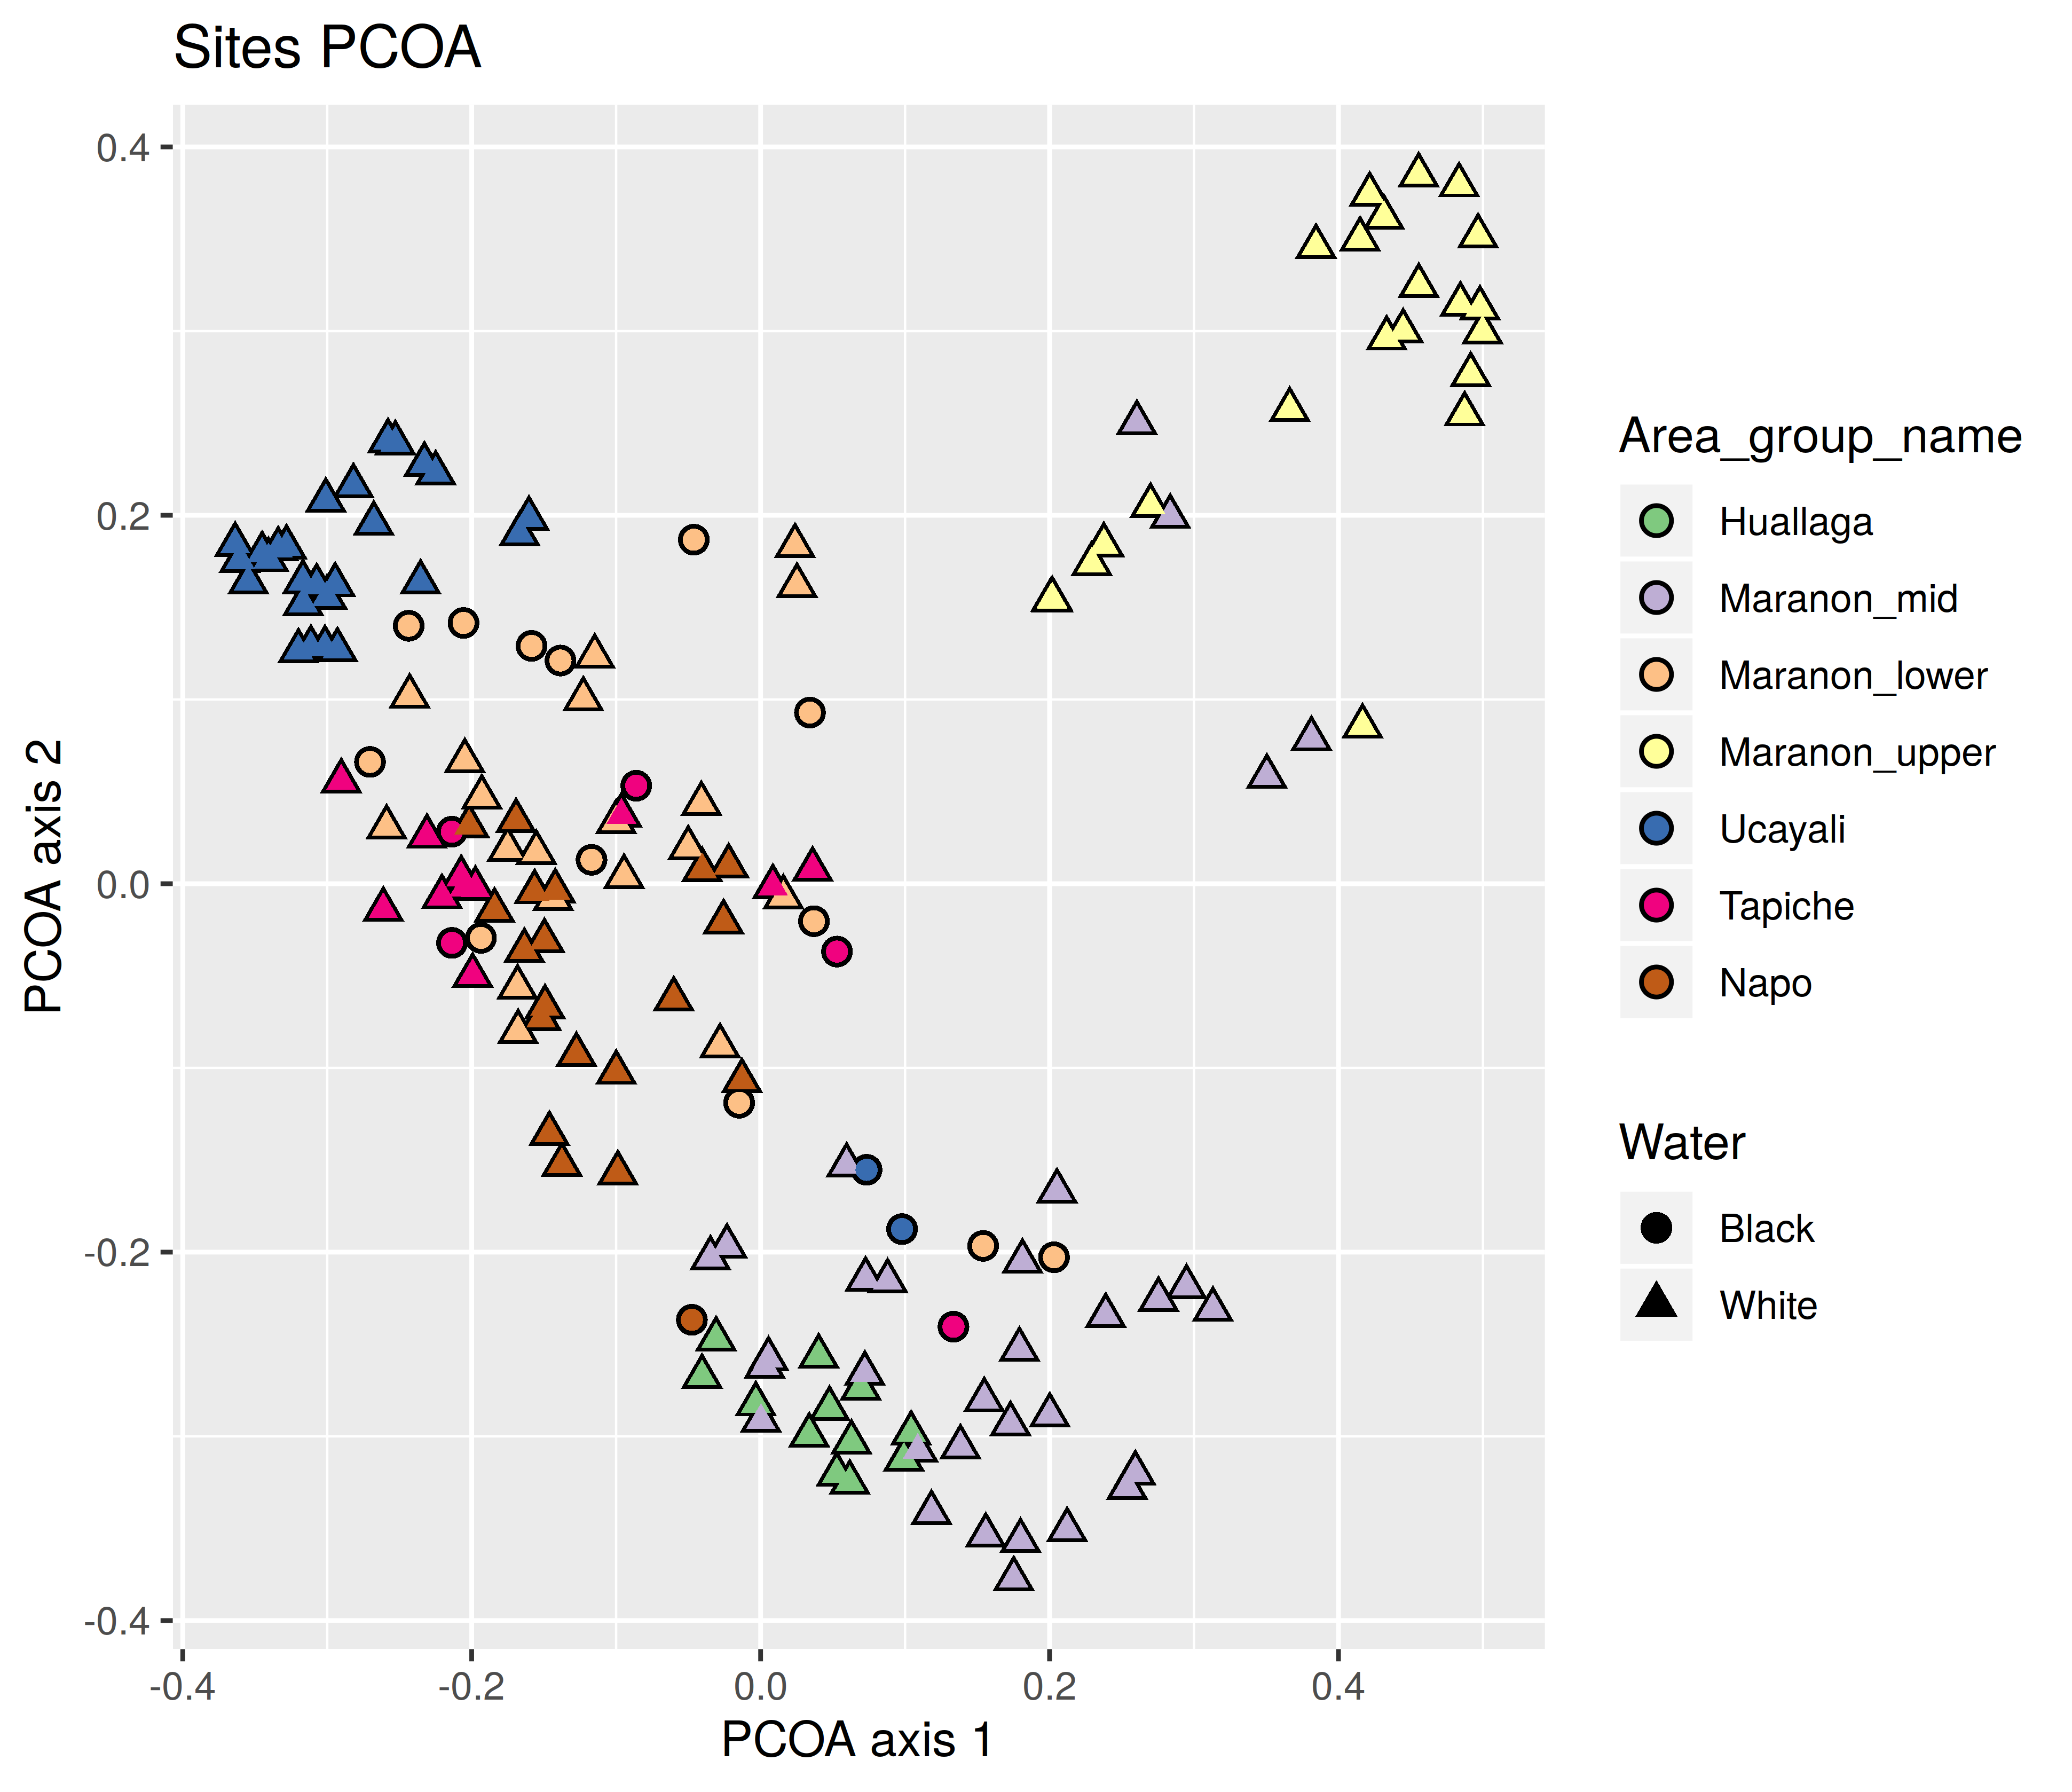
\includegraphics[width = 0.7\textwidth]{pcoaotu12}
\caption{First 2 dimensions of PCoA performed on the full OTU table using the Bray Curtis statistic as the distance metric. The 2 axes account for 19.8\% of the variance.}
\label{fig:pcoaotu12}
\end{figure}

To illustrate the effect of measures on the PCoA algorithm, we produced 2 dimensional ordination plots for the Euclidean and the Jaccard metrics. The Euclidean metric has the form given in equation \eqref{eq:euclideanmetric} and the ordination plot (see Figure \ref{fig:pcoaeuc}) has the same form as the one obtained using PCA. The only difference is the scale (the covariance matrix is divided by the number of samples) and the reflection of the points on the x-axis. The Jaccard metric is given by
\begin{equation}
Jac_{ij} =\frac{2C_{ij}}{1-C_{ij}},
\end{equation} 
where $C_{ij}$ is the Bray-Curtis statistic between sample $i$ and $j$. The ordination plot produced using this index is shown in Figure \ref{fig:pcoajac}.

%%RESULTS of PCoA with different metrics
\begin{figure}[h]
\centering
\begin{subfigure}{0.4\textwidth}
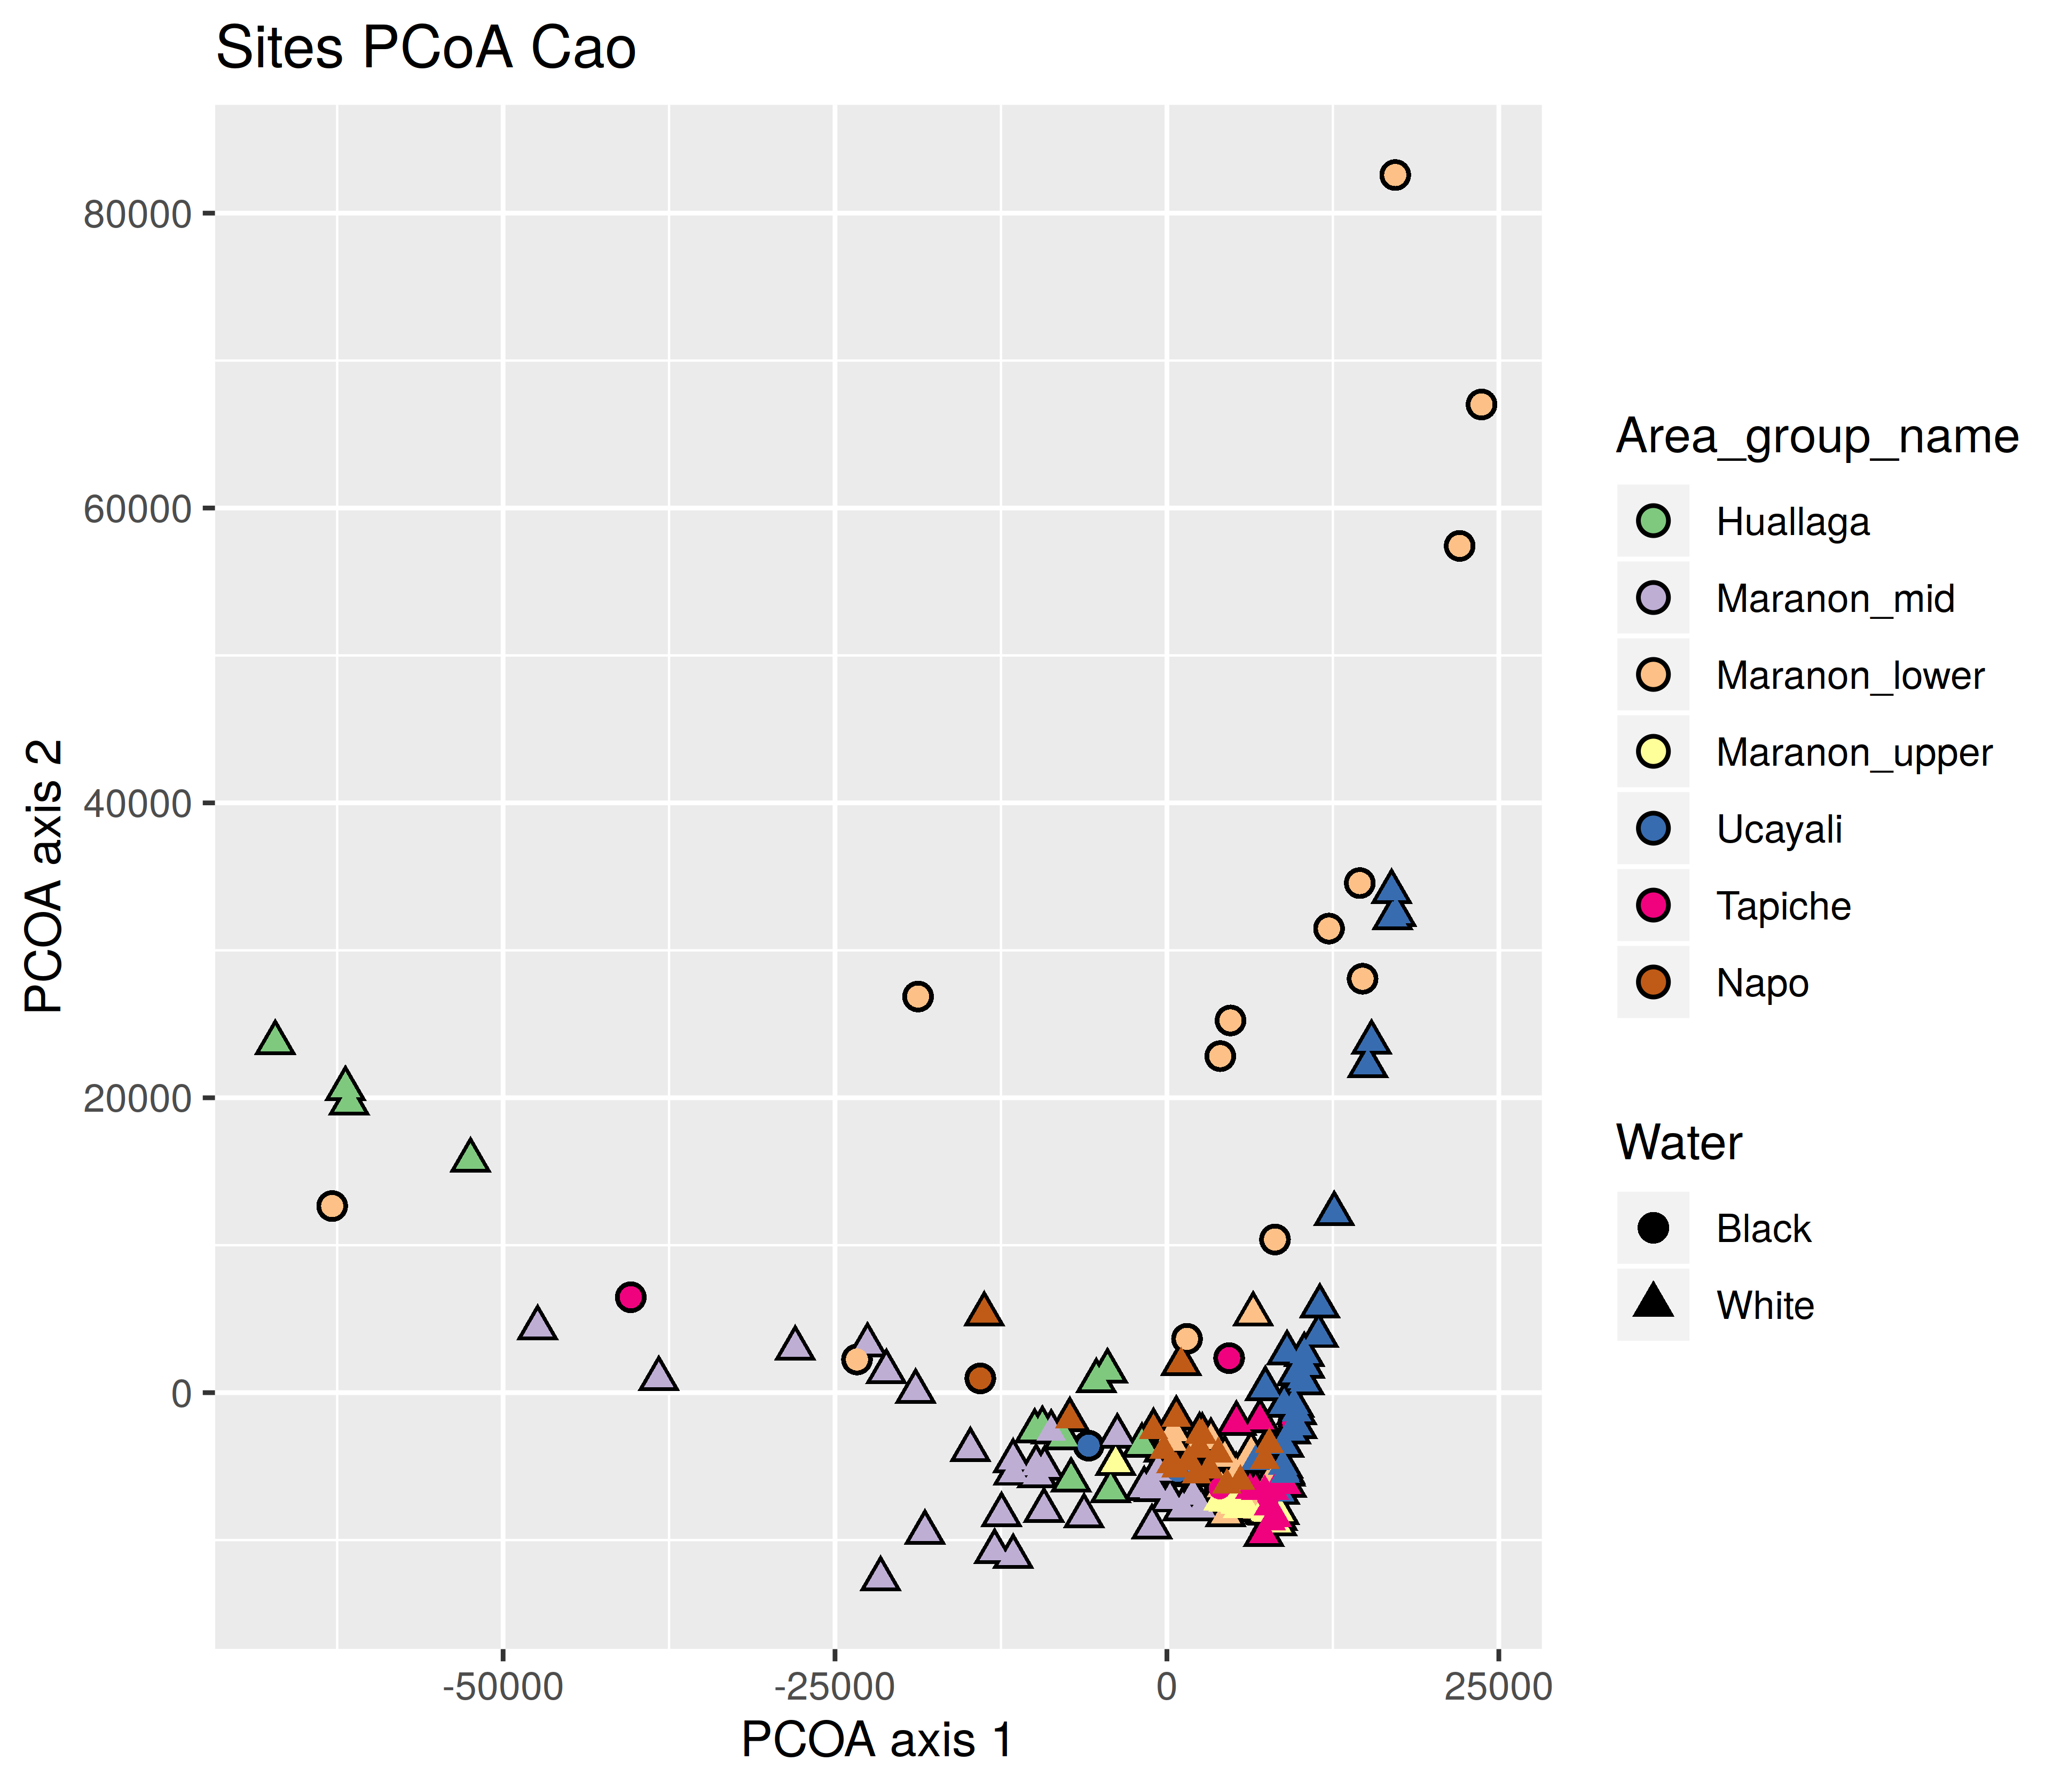
\includegraphics[width = \textwidth]{pcoa12eucotu}
\caption{PCoA using the Euclidean Metric. The result is the same as with PCA; only the scales have different values and the points are flipped over the X-axis.}
\end{subfigure}
\label{fig:pcoaeuc}
\begin{subfigure}{ 0.4\textwidth}
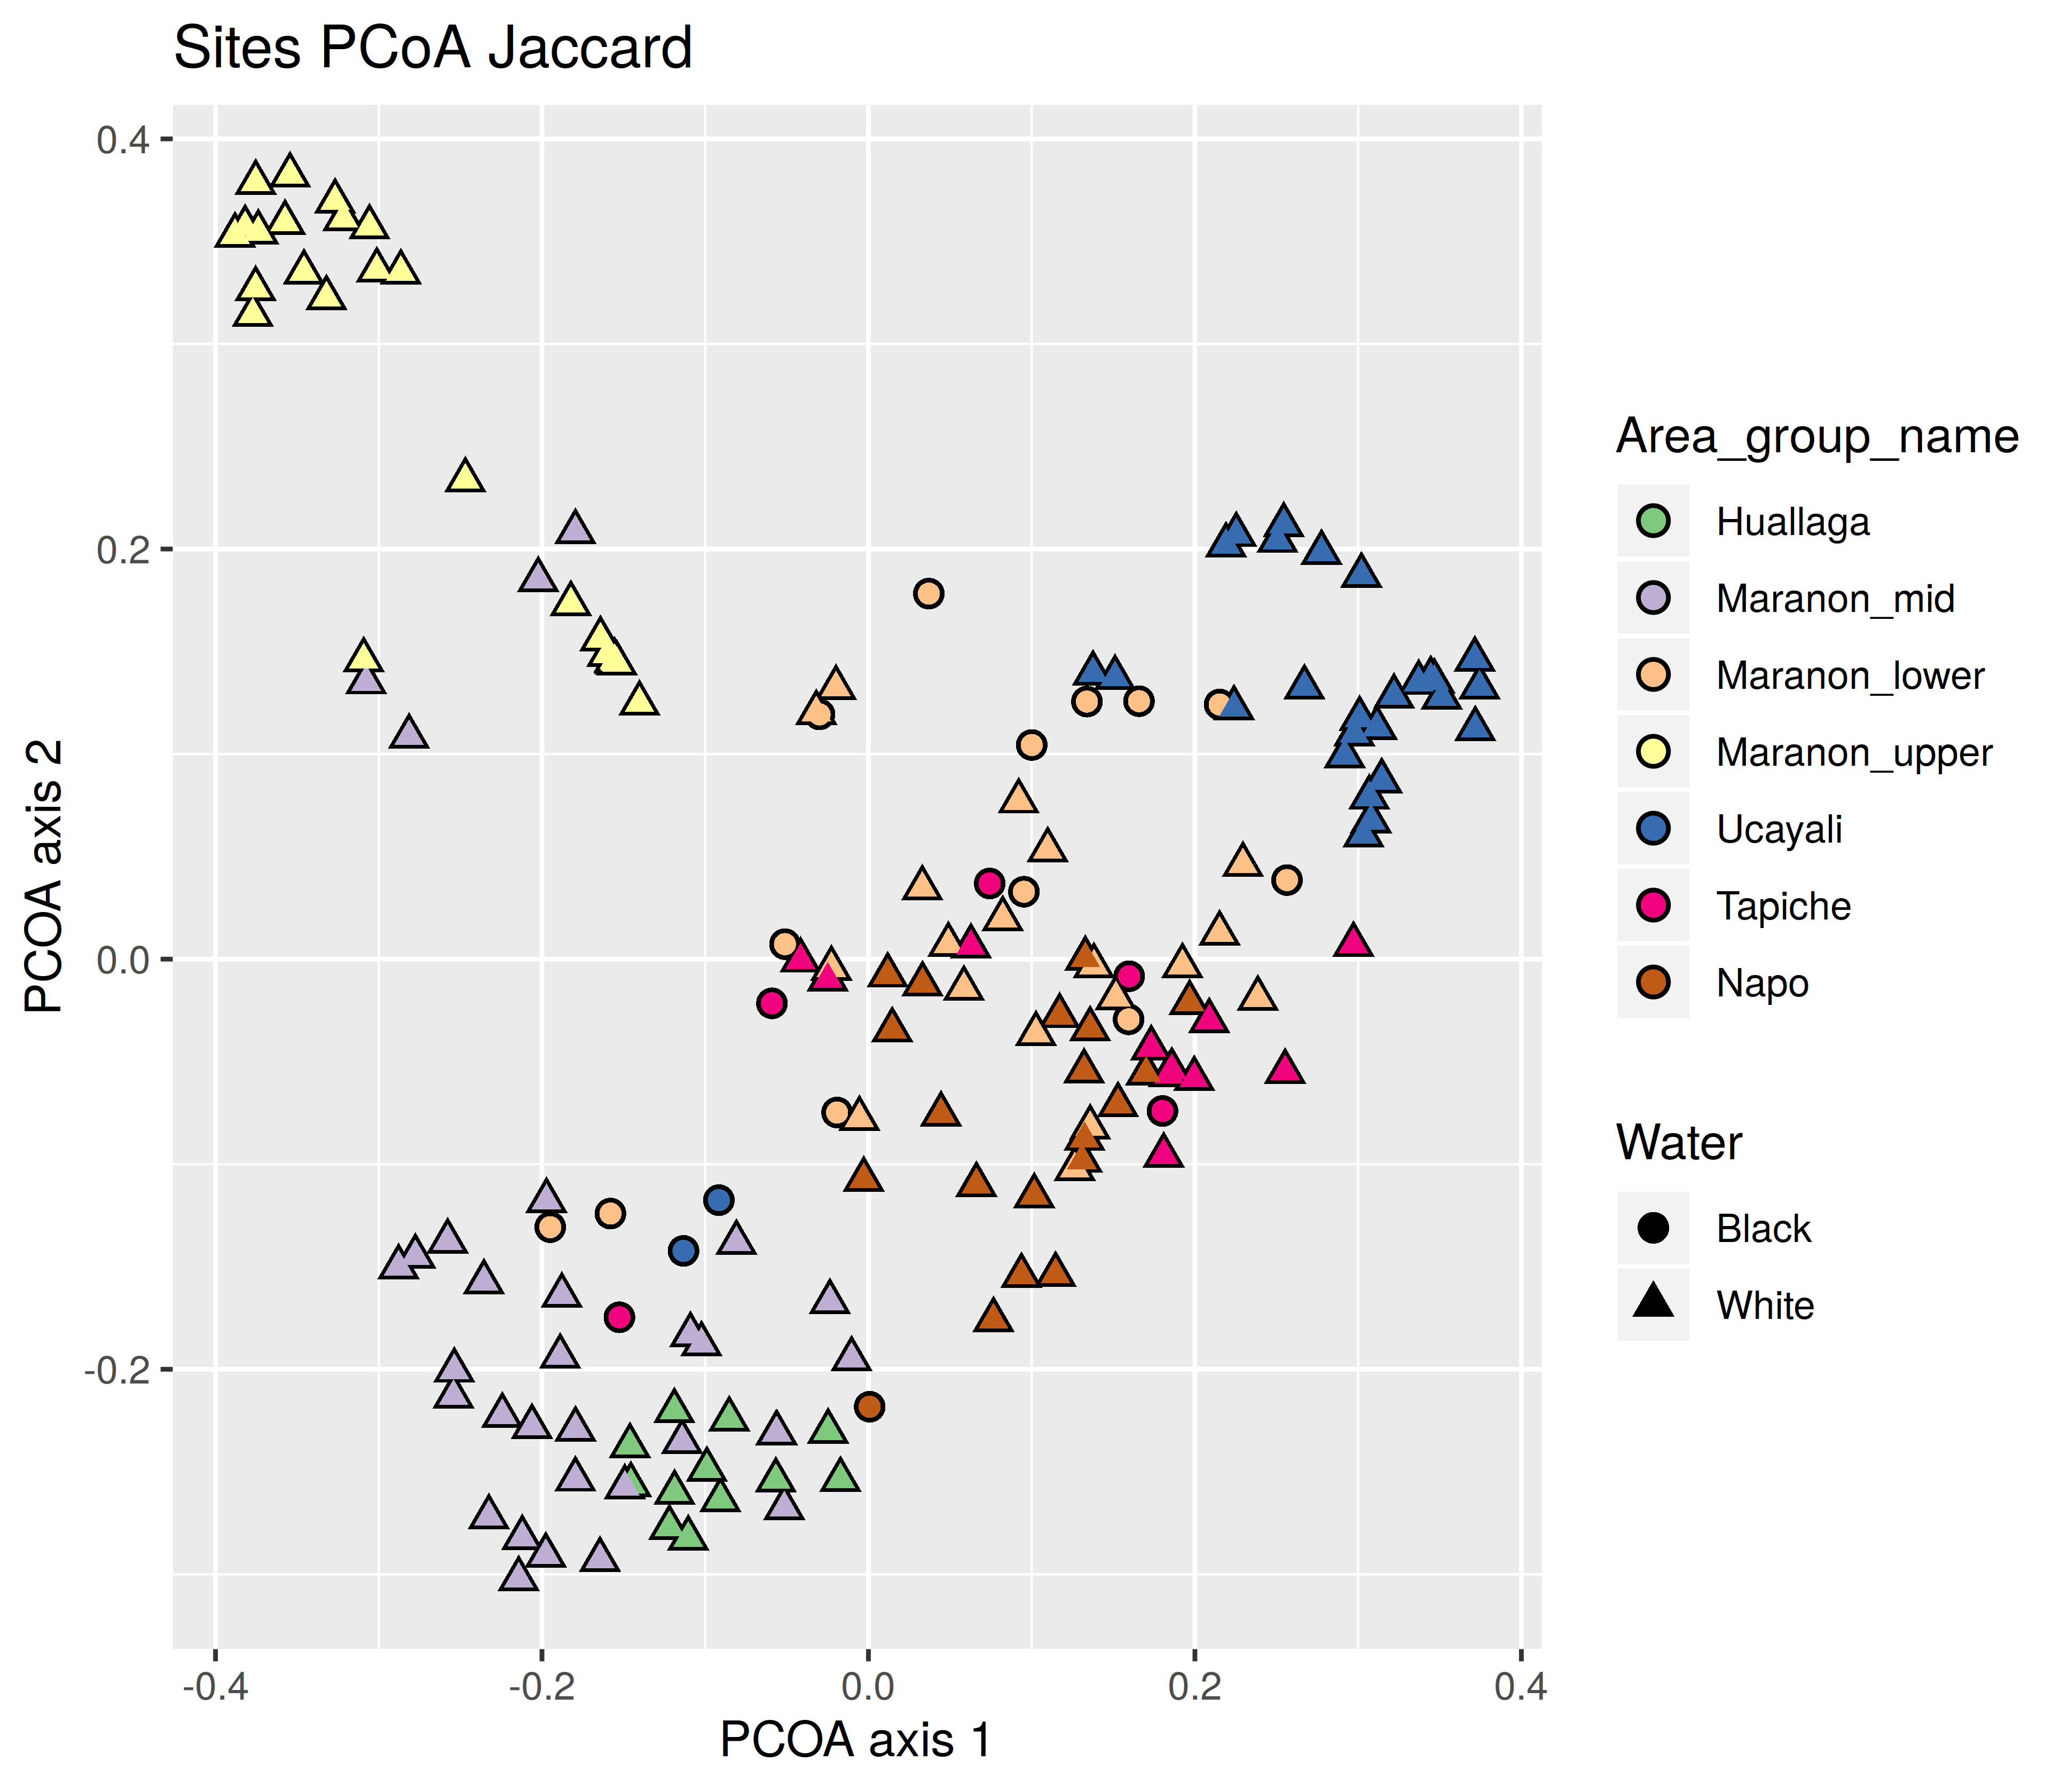
\includegraphics[width = \textwidth]{pcoa12jacotu}
\caption{PCoA using the Jaccard metric. The result is similar with the one obtained using Bray-Curtis. Both measures are rank-order similar.}
\label{fig:pcoajac}
\end{subfigure}
\end{figure}
%Motivate NMDS
%EG actual distances are not that important so NMDS might be more usefull which maximisies correlation
%% NMDS
%%%Explain similarity of NMDS with PCOA

% Uncomment this line, when you have siunitx package loaded.
%The SI Units for dynamic viscosity is \si{\newton\second\per\metre\squared}.
% \begin{figure}[htbp!] 
% \centering    
% \includegraphics[width=1.0\textwidth]{minion}
% \caption[Minion]{This is just a long figure caption for the minion in Despicable Me from Pixar}
% \label{fig:minion}
% \end{figure}
\subsection{NMDS}
\section{Data processing}
\subsection{Normalisation}

Count data from amplicon sequencing display a very high degree of variability in total read counts per sample \cite{inadmissible_rareying}. A histogram, Figure \ref{fig:counthistogram}, of the samples' total count reads for our data exemplifies this variability. The sums range from 17 to 219113, with a median and mean of 63672 and 77152 respectively. This much variation between samples makes it hard to identify which OTUs' difference in abundance between samples is significant and also might negatively impact the performance of the classifiers. 
 
 The increased variation comes from a systematic variability affecting multiple samples and OTUs in a similar manner. Sources of such variability can be the inconsistencies in DNA extraction and handling of samples,  a varying quality of sequencing runs \cite{pereira_comparison_2018}, and other PCR-specific amplification biases (like primer mismatch, GC-content etc.) \cite{abundance_nodate,krehenwinkel_estimating_2017}.
 
 Furthermore, these biases can cause the distribution of read counts obtained from high-throughput amplicon sequencing to diverge significantly from the actual distribution of species abundances in the same samples. The Pearson correlation between read and species frequencies is close to zero \cite{edgar_unbias:_2017}.
 
 The removal of this Systematic Variability is called \textit{Normalisation} and it's original aim in the bioinformatics literature is to increase the statistical power and false positive rates of differential abundance analysis \footnote{Differential abundance analysis aims at finding OTUs (or genes in the case of metagenomic studies) whose variation between groups of samples (e.g. black and white water river samples) is statistically significant.}. We will be testing if normalisation methods have any effect on the classifiers' scores.
 
 A normalisation method that produced promising results in differential analysis on datasets similar to ours is Cumulative sum scaling (CSS). This method is an extension to the quantile normalisation approach which divided read counts by the $Q$th percentile of each sample’s non-zero count distribution. CSS determines that percentile using a data-driven approach\cite{css_diff_abund}.
 
 To illustrate how normalisation methods work we define $X_{i,j}$ as the read counts of sample  $i =1,...,n$ and OTU $j=1,...,p$. The normalisation factor of the total sum scaling (TSS) method is found by summing the read counts in a sample $i$:
 \begin{equation}
 	N_i = \sum_{j=1}^{p} X_{ij}.
 \end{equation}
Then the counts in row $i$ of the read matrix $X$ are divided by the factor $N_i$. TSS is the most commonly used method of normalisation but it has been shown to introduce biases in differential analysis estimates \cite{bullard_evaluation_2010}.

Quantile scaling computes the normalisation factor by taking into account how OTU total counts (for all samples) vary, and choosing a percentile that produces desirable properties (such as robustness from highly abundant OTUs).
The scaling factor is defined as:
\begin{align}
	N_i &= \underset{ j \in G}{ Q\text{th quantile}} \  X_{ij}\\
	G  &= \left\{ j : \sum_{i = 1}^{n} X_{ij} > 0\right\}.
\end{align}

 
\begin{figure}[htb]
\centering
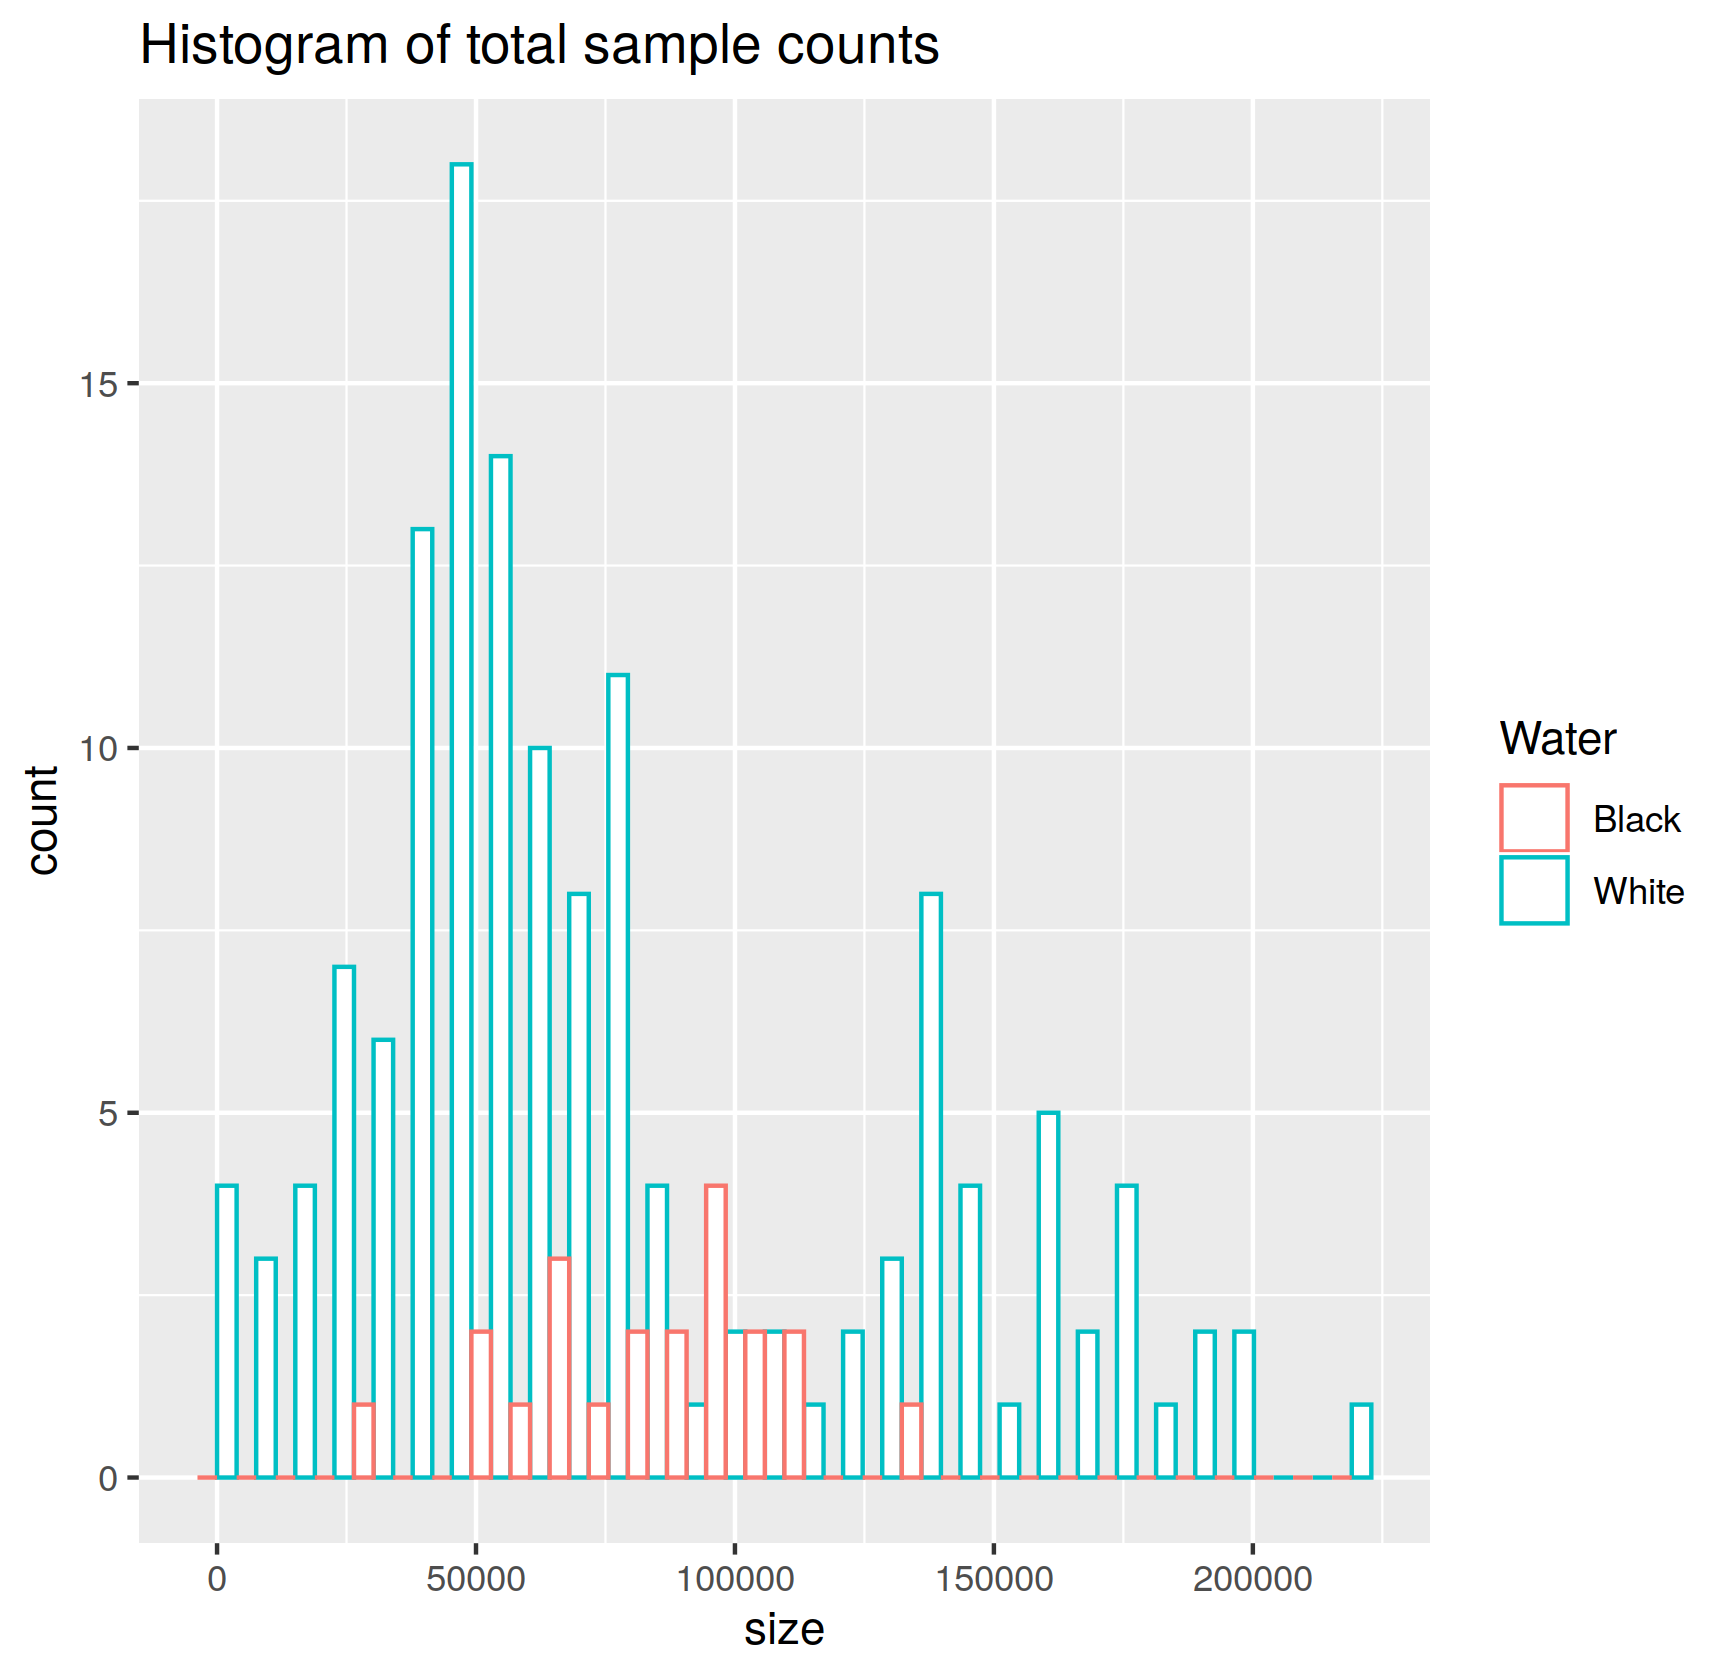
\includegraphics[width = 0.7\textwidth]{histogramofcountdata}
\caption{Histogram of the sum of OTU counts of each sample. The cyan colour represents white water samples and the red colour black water samples.}
\label{fig:counthistogram}
\end{figure}

CSS normalisation involves the calculation of a data-driven quantile 
We define the $l$th quantile of sample $i$ as $q_i^l$, which means that $l$ OTUs have a read count lower than $q_i^l$. Also we define the sum of counts per samples $i$ up to the $l$th quantile as
\begin{equation}
	s_{i}^{l}=\sum_{j|X_{ij} \leq q_{i}^{l}} X_{ij}.
\end{equation} 
With this notation, the total sum normalising factor is given by $N_i = s_i^p$ (where $p$ is the total number of OTUs). CSS chooses a value $\hat{l} \leq p$ using a data driven approach to calculate the scaling factor ($N_i = s_i^{\hat{l}}$) for each sample and get normalised counts.
In particular, the quantile $\hat{l}$ for the threshold $q_i^{\hat{l}}$ is chosen  to be the smallest value where the median absolute deviation of sample-specific quantiles $q_i^l$ from a reference point (the median quantile $q_i^l$ across all samples) shows high instability. \cite{css_diff_abund}.
% web

% CSS + LOG histograms 
\begin{figure}[h]
	\centering
	\begin{subfigure}{0.4\textwidth}
		\centering
		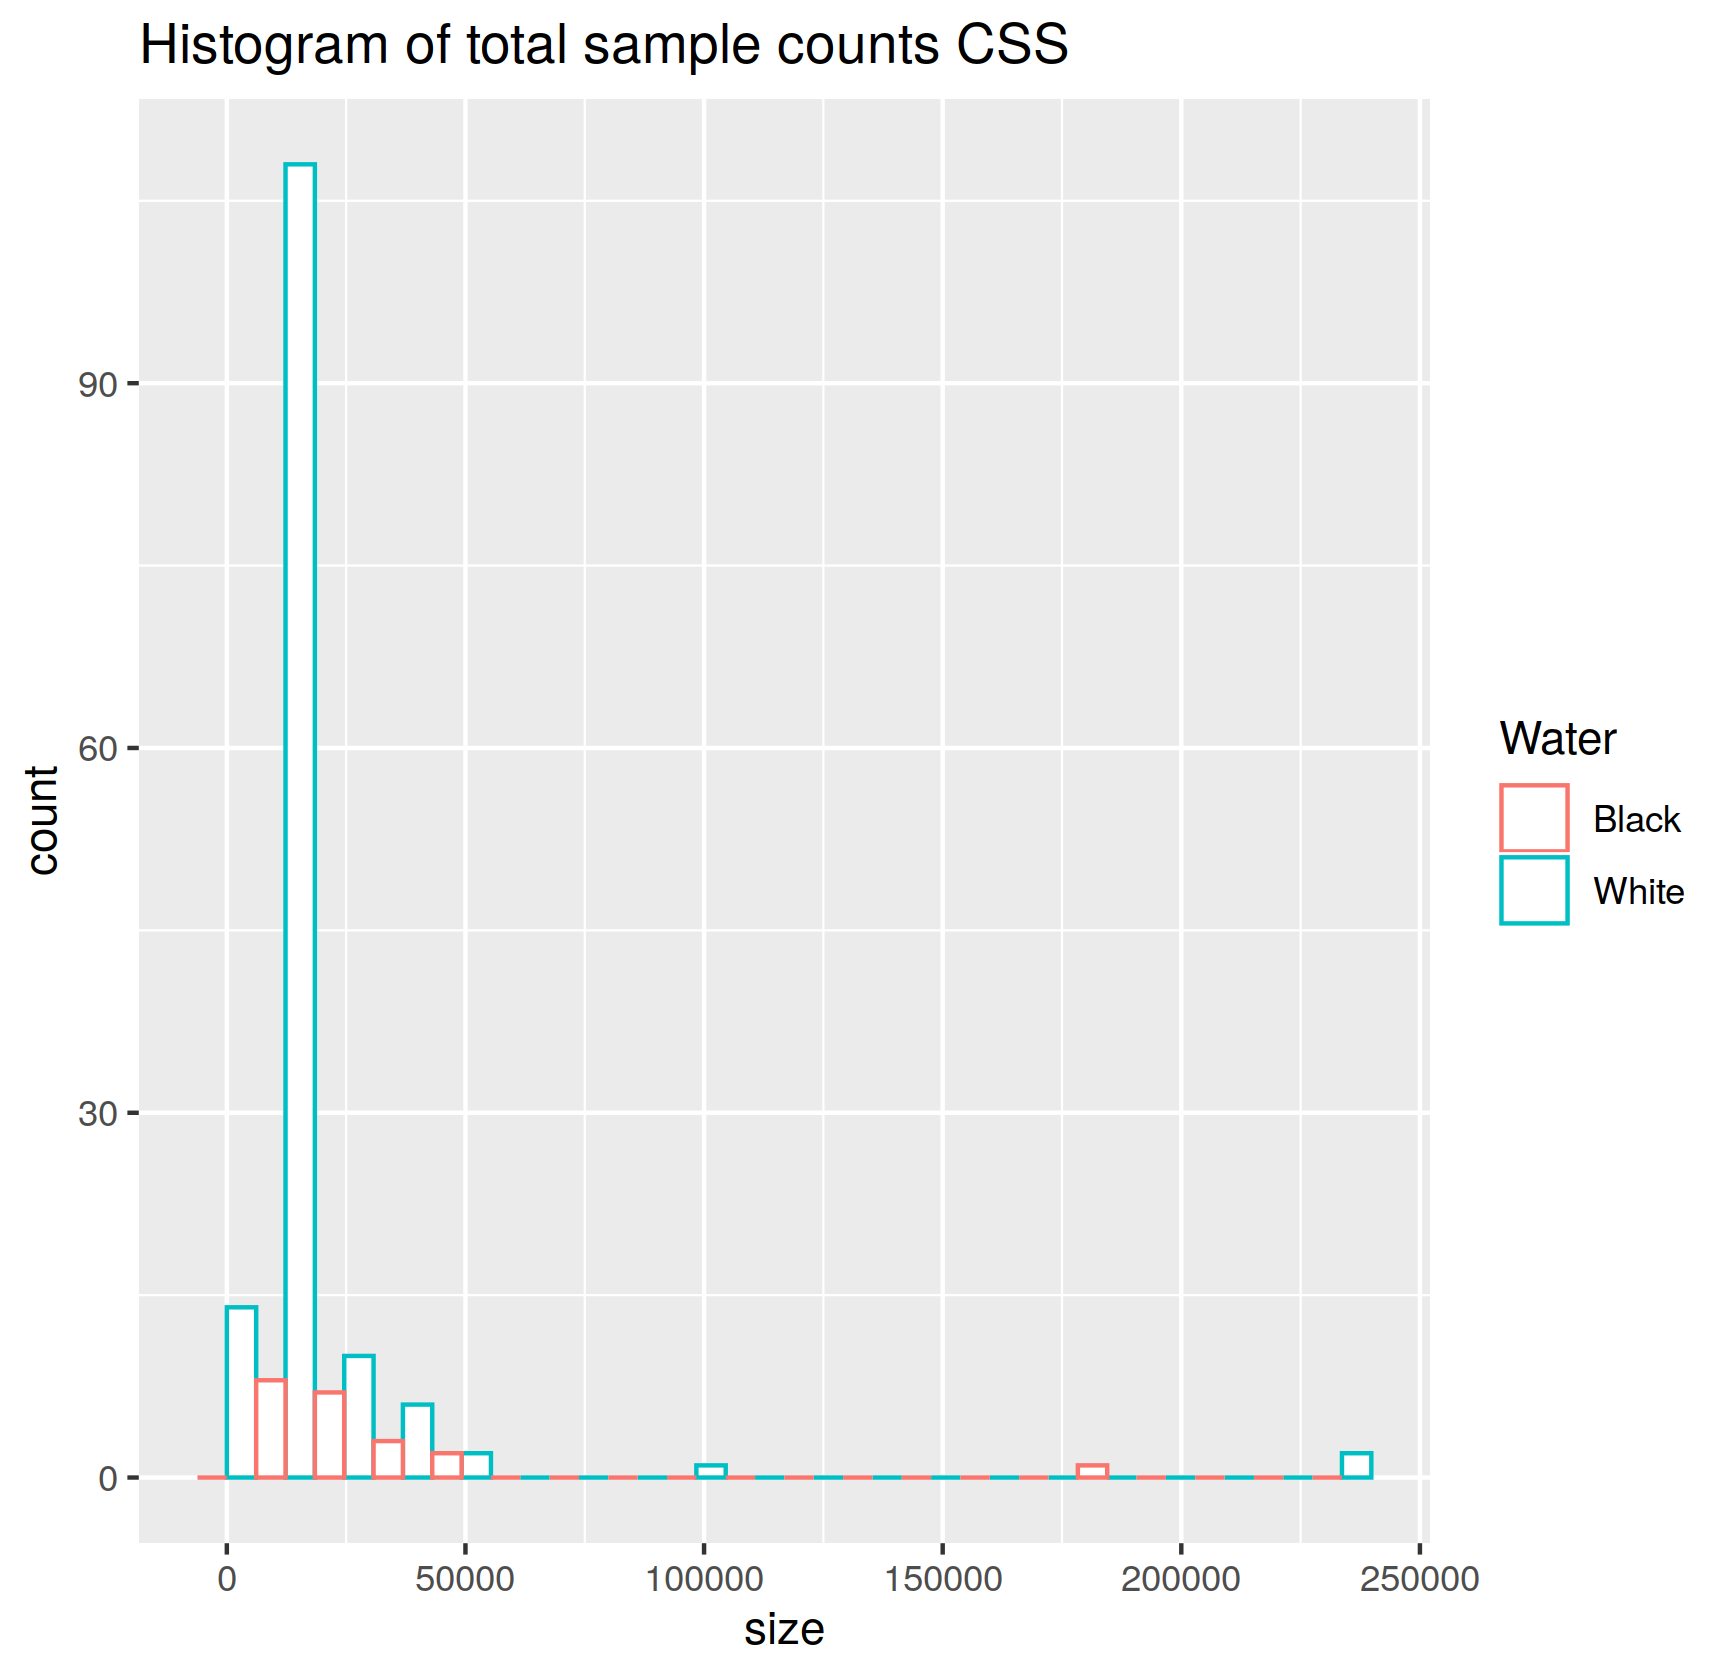
\includegraphics[width = \textwidth]{histogramofcountdatacss}
		\caption{}
		\label{fig:histcss}
	\end{subfigure}
	\begin{subfigure}{0.4\textwidth}
	\centering
	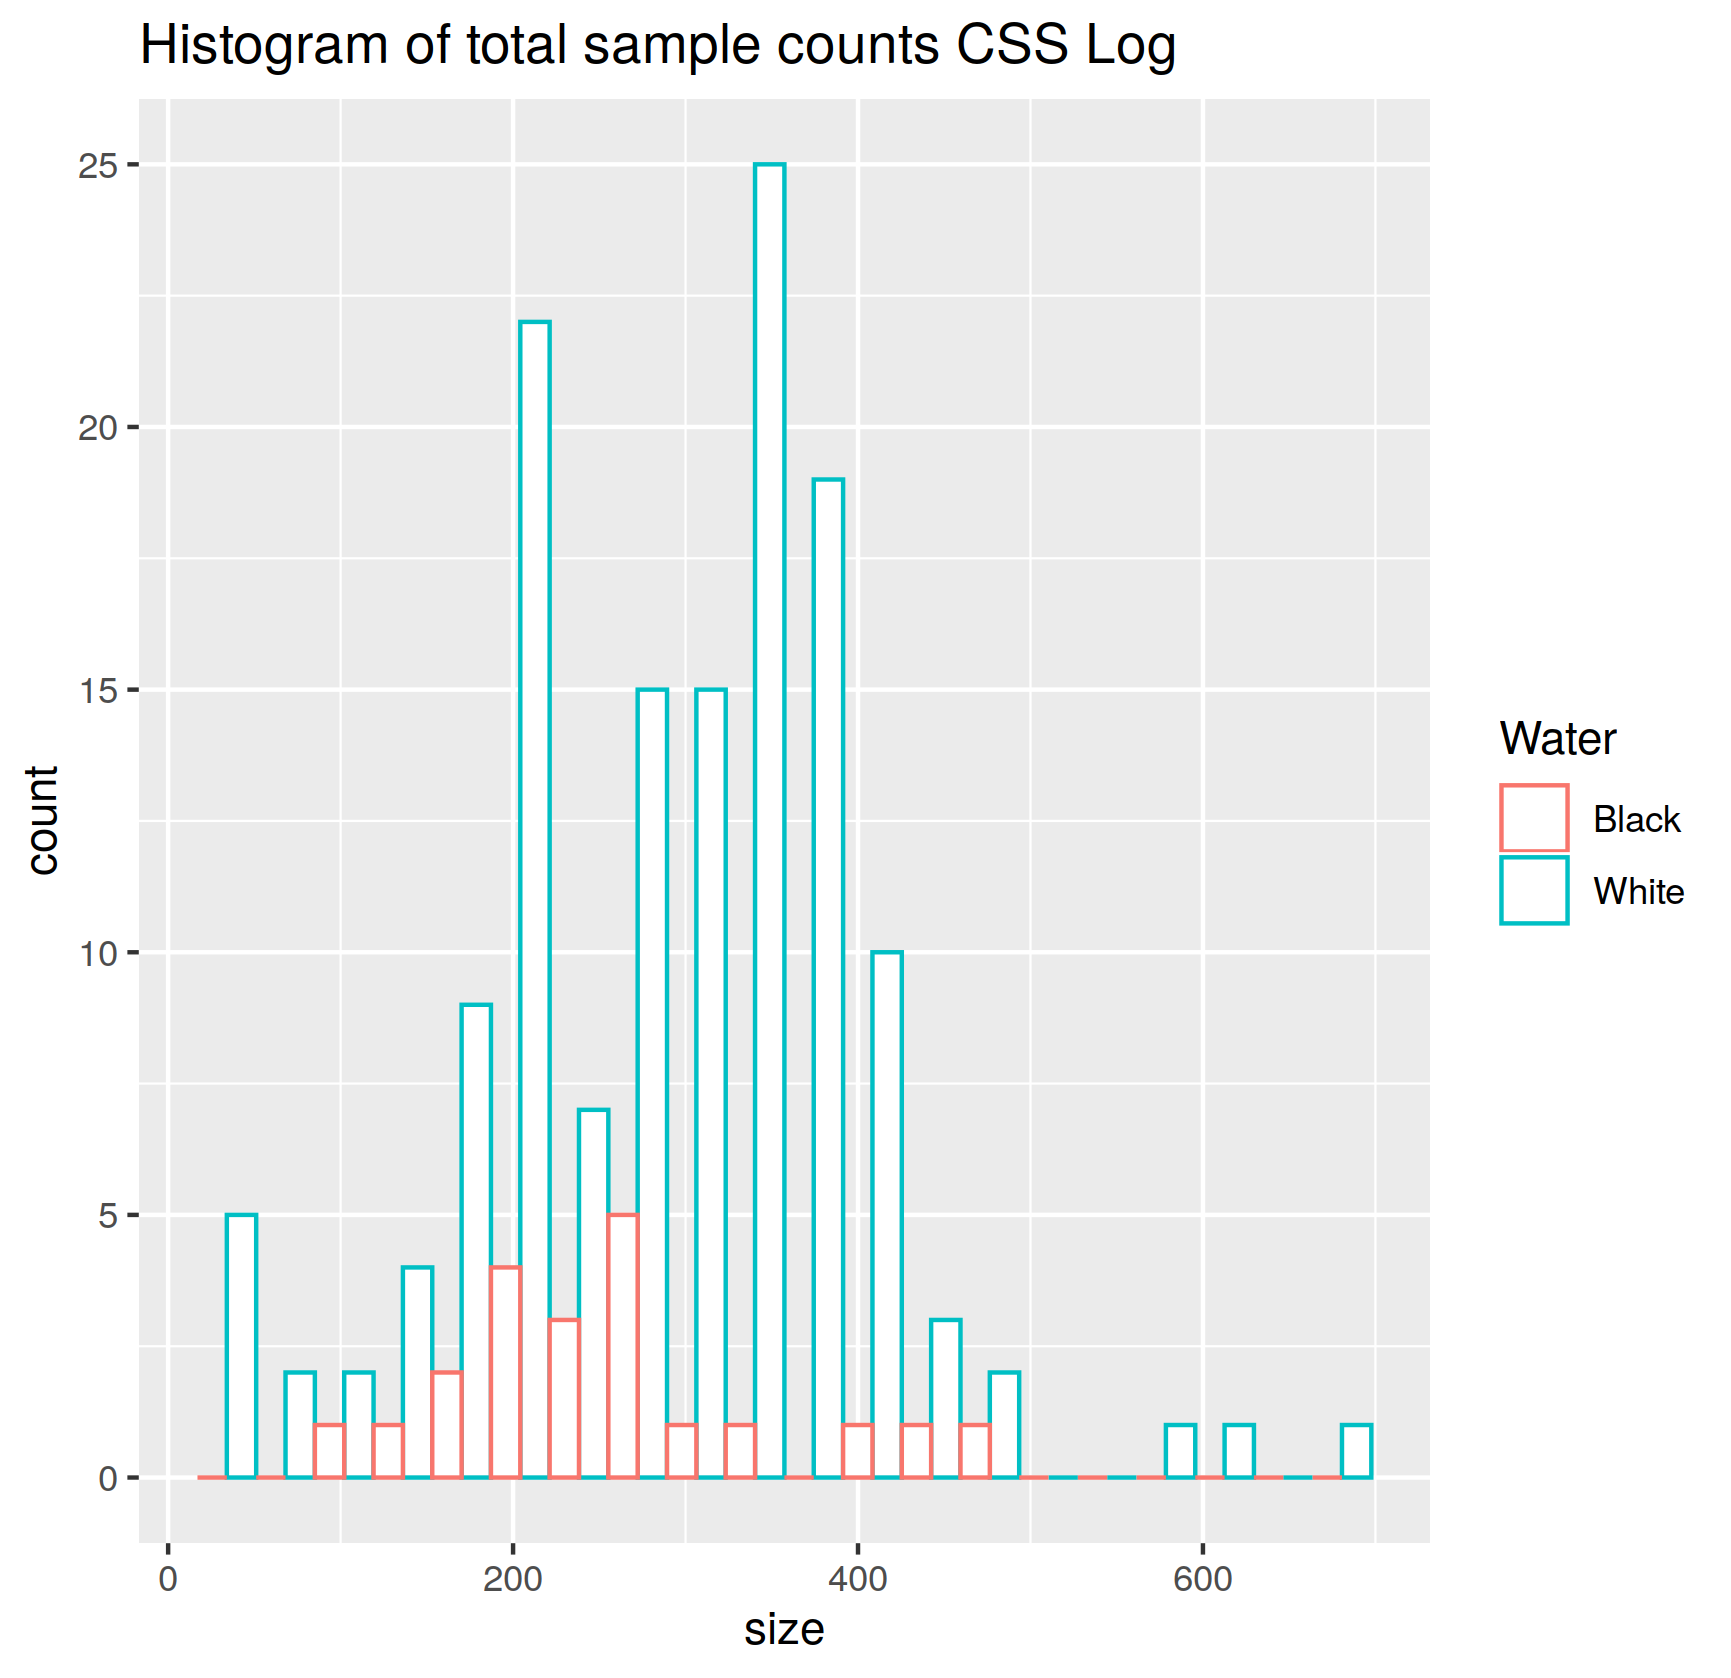
\includegraphics[width = \textwidth]{histogramofcountdatacsslog}
	\caption{}
	\label{fig:histcsslog}
	\end{subfigure}
	\caption{Histogram of the read counts per sample after \ref{fig:histcss} CSS normalisation and with \ref{fig:histcsslog} a $log_2$ transformation. The cyan colour represents white water samples and the red colour black water samples. }
\end{figure}


After applying the CSS normalisation, the variation of read counts per samples drops significantly (except for some samples whose total read counts increase, see Figure \ref{fig:histcss}). Applying a $log_2$ transformation to the data after normalising reduces the variation drops even more (see Figure \ref{fig:histcsslog}). Furthermore, performing PCoA and NMDS (Figure \ref{fig:pcoa12otucss} and \ref{fig:nmds12otucss} respectively) on the normalised data separates white and black water samples better than if the normalisation was not applied. However, doing the same on the $log_2$ transformed data doesn't have the same effect.

\begin{figure}[h]
	\centering
	\begin{subfigure}{0.4\textwidth}
		\centering
		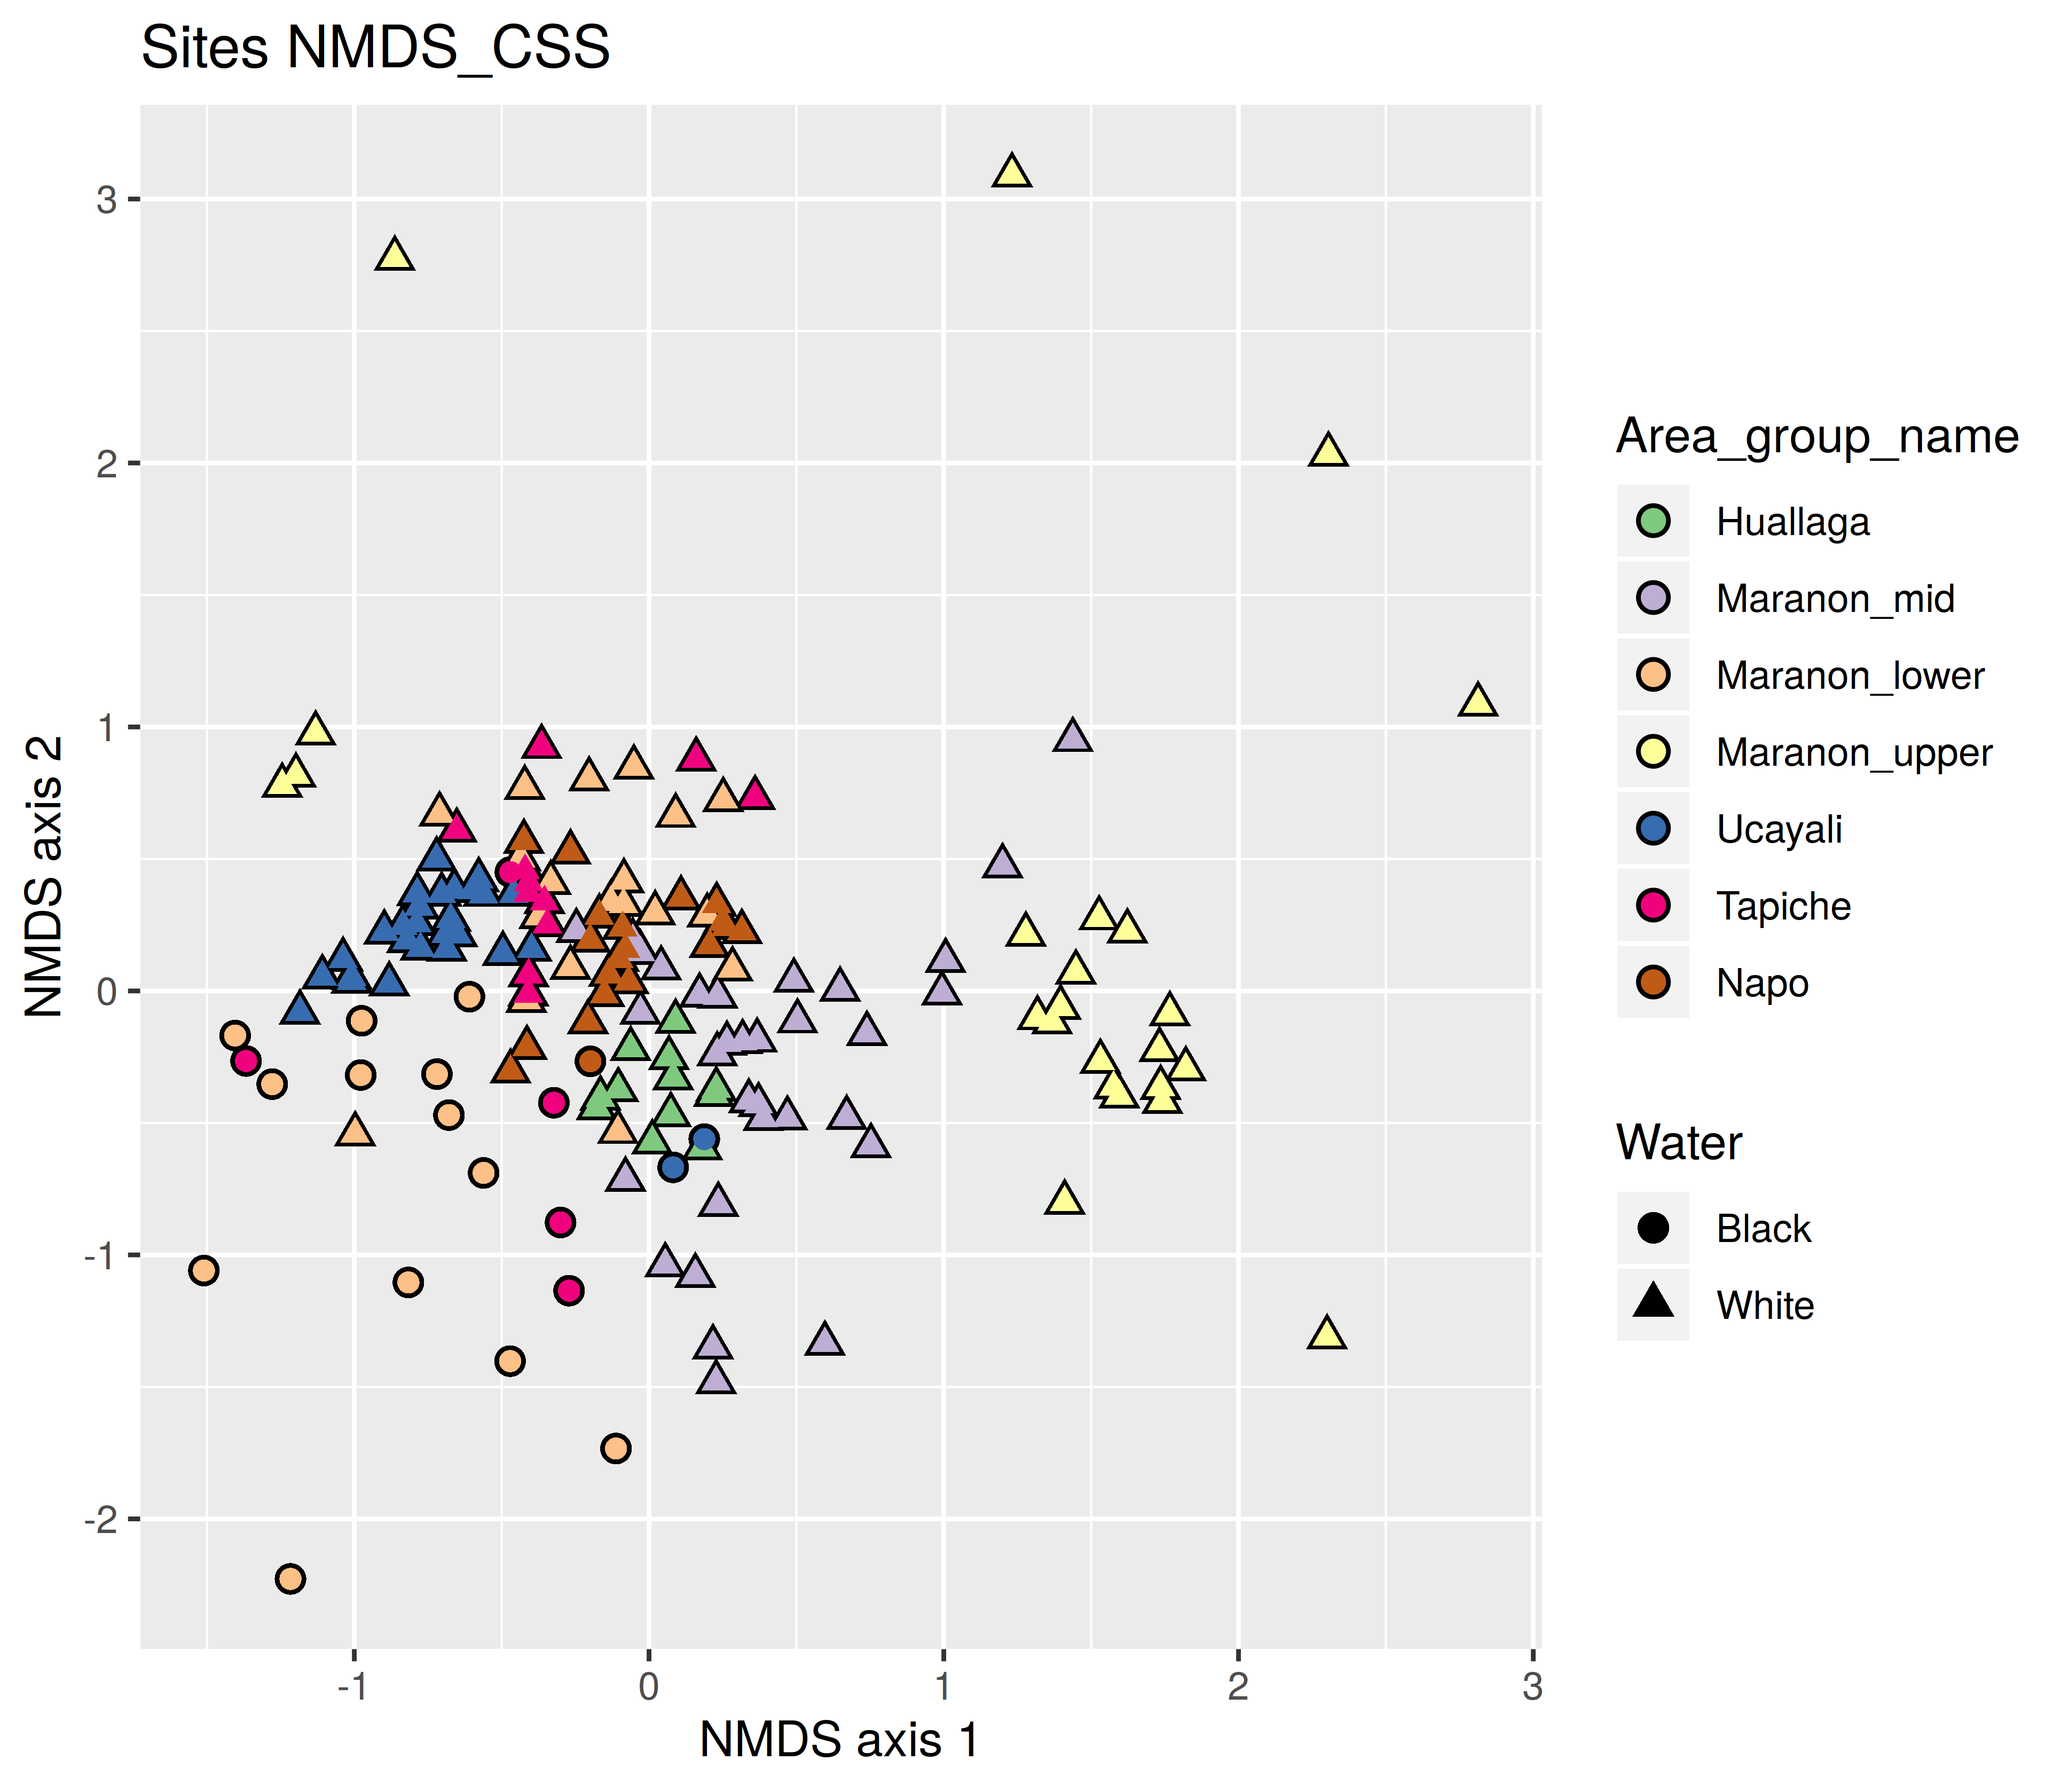
\includegraphics[width = \textwidth]{nmds12otucss}
		\caption{}
		\label{fig:nmds12otucss}
	\end{subfigure}
	\begin{subfigure}{0.4\textwidth}
		\centering
		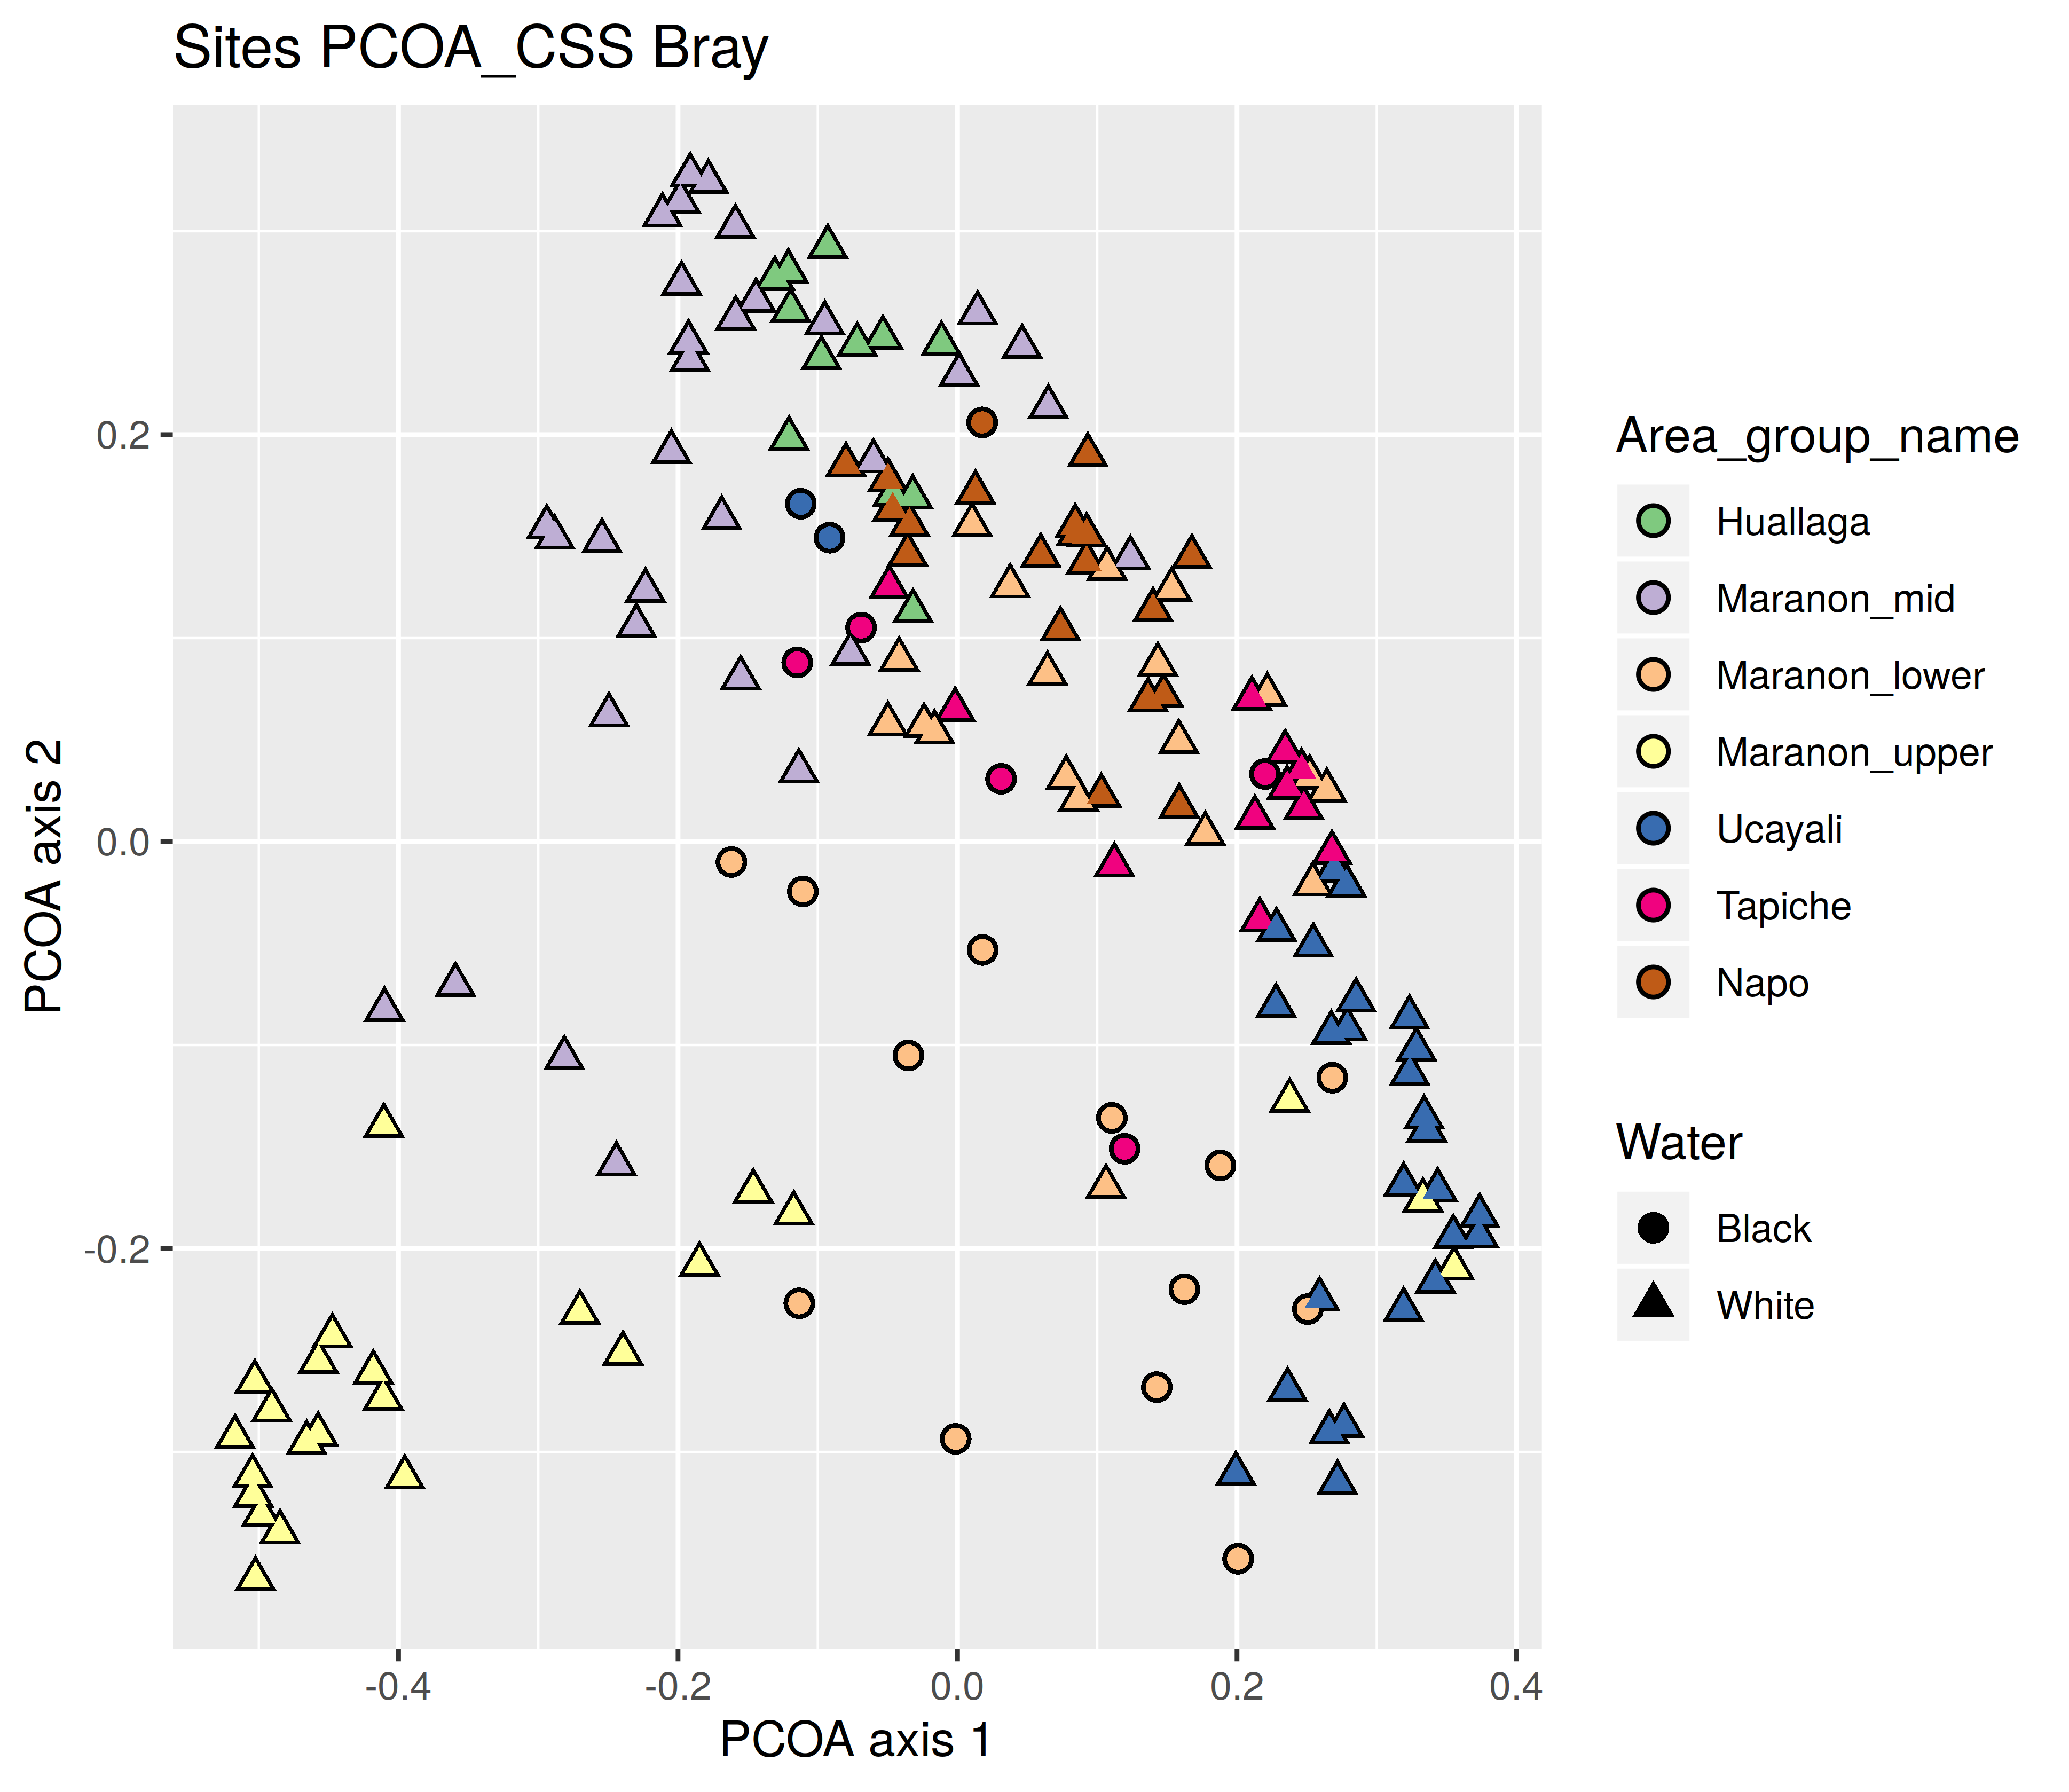
\includegraphics[width = \textwidth]{pcoa12otucss}
		\caption{}
		\label{fig:pcoa12otucss}
	\end{subfigure}
	\caption{Ordination plots for the CSS normalised data. \ref{fig:nmds12otucss} shows an NMDS plot of the data and \ref{fig:pcoa12otucss} a PCoA using Bray-Curtis measure. Both methods separate white and black water samples better than their respective ordination methods applied to non-normalised data.}
\end{figure}

We will be checking if this normalisation method and transformation produces any significant improvements (over the unnormalised dataset) in the classifiers ability to determine the river colour. 

%%Normalization, which is the process where systematic variability is identified and removed, is therefore a vital part of the data analysis. 
%https://www.ncbi.nlm.nih.gov/pmc/articles/PMC5910605/
% A substantial part of this variability is systematic and affects multiple genes and/or samples in a similar way. One example of systematic variability is the differences in sequence depth, where each sample is represented by a varying number of reads [13]. Systematic variability also comes from other technical sources, such as inconsistencies in the DNA extraction and sample handling, varying quality between sequencing runs, errors in the read mapping, and incompleteness of the reference databasescd 


\subsection{Feature Correlation}

A big minority of OTUs in our data set have been found to have an absolute Spearman correlation of more than 0.9 with at least one other OTU. This correlation has a biological underpinning as it is expected that the abundance of species in a river environment would co-vary along it's length. Relationships between species in an environment have been modelled and can take many forms, like parasitic (the abundance of OTU1 and OTU2 is increased and decreased and they are both present), competitive (the abundance of both OTU1 and OTU2 is decreased when they are both present), and mutual (the abundance of both OTU1 and OTU2 is increased when they are both present). More complicated, non-linear correlation networks exist in nature between more than two species that are very difficult to capture even with large amounts of unbiased data \cite{weiss_correlation_2016}. 



For our problem at hand, recovering such correlation networks is not of interest. We are more interested in selecting the best features from our data that would aid in the classification. Thus, we used the Spearman correlation with a threshold of 0.9 to remove 122 OTUs to create a new data set without highly correlated OTUs. 








\section{PERMANOVA}
\section{Machine Learning}
\subsection{Logistic Regression}
\subsection{Random Forests}
\section{Data-Splitting}

Together with the OTU table, our data also include the location of the samples in the rivers (in Easting and Northing coordinates) and in which part of the river they belong to. Because of this location attribute, our samples cannot be said to be independent. Thus, the way we choose to split our data into training and testing sets will surely affect the accuracy of the classifier. For example, testing on a set that is composed of samples maximally distant from the ones in the training set (see Figure \ref{fig:groupsamp}) will produce different results than testing on a set with all samples in close proximity to the ones in the training set (see Figure \ref{fig:stratsampl}).

To avoid choosing a split method, several ones have been employed that represented different splitting conditions. The classifiers have then been tested on all of them so as to evaluate how well they can perform under various circumstances.
%% Stratified an group folds for tain test split plot
\begin{figure}[h]
\centering
\begin{subfigure}{0.4\textwidth}
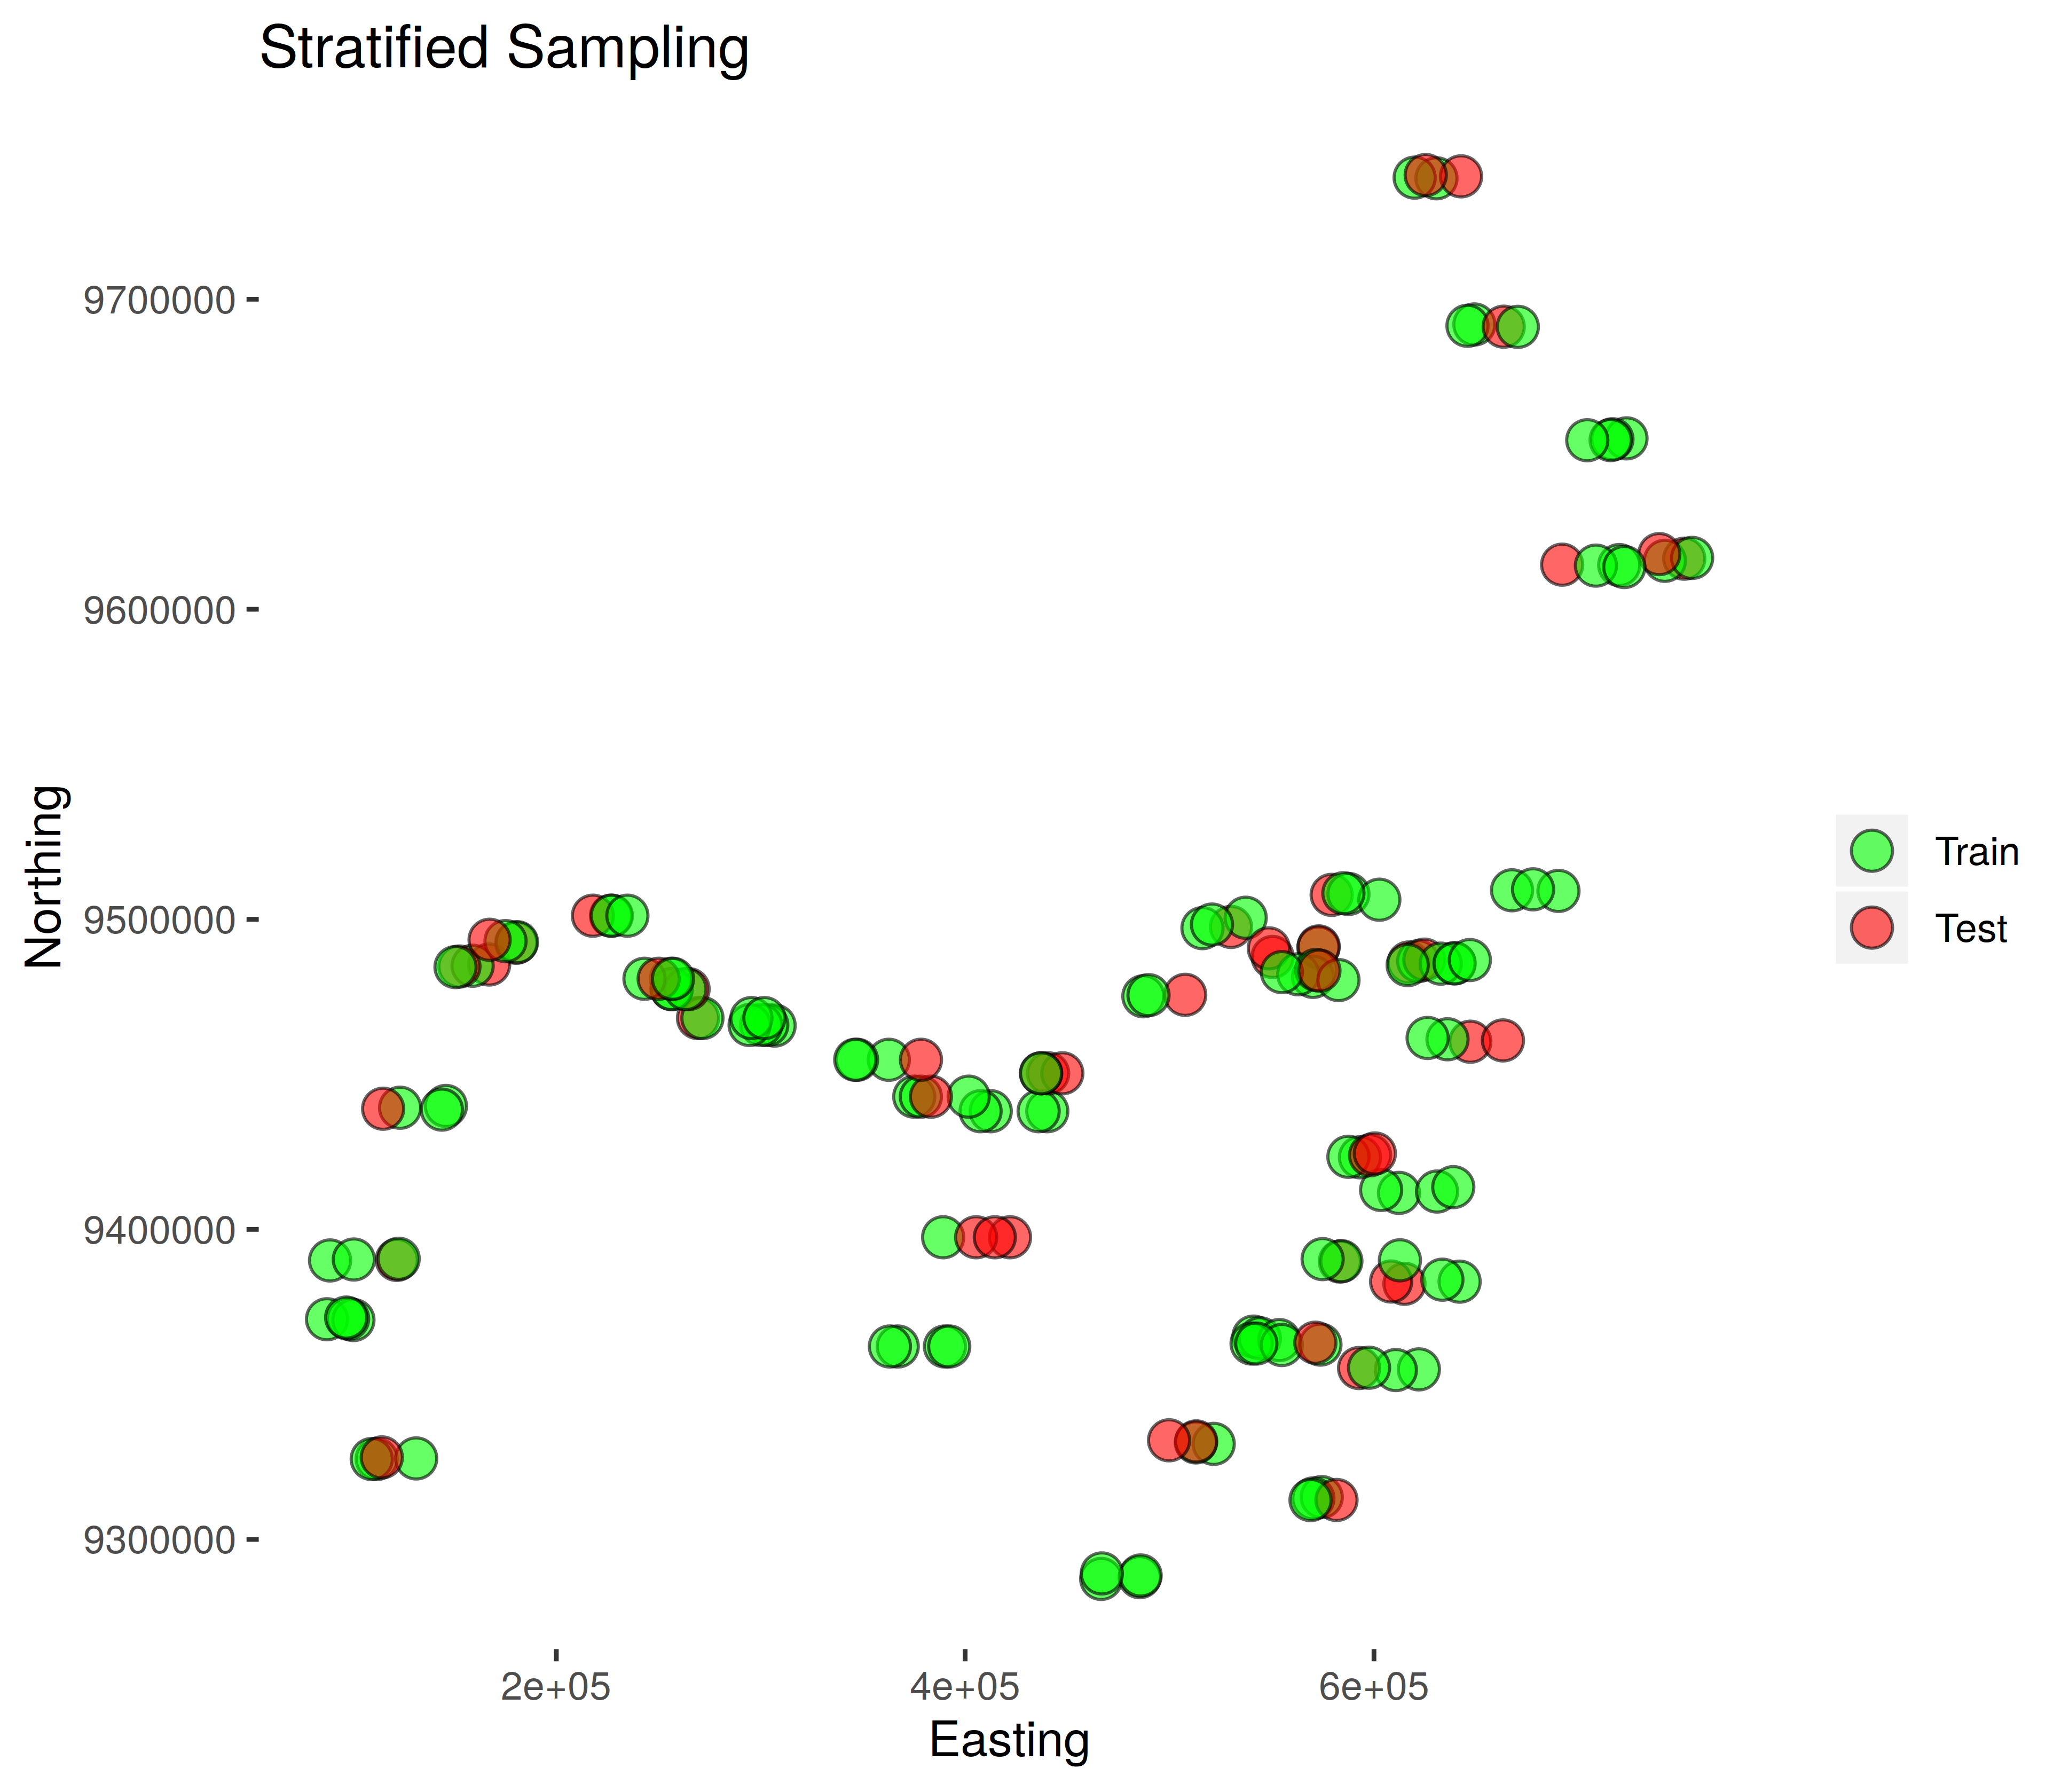
\includegraphics[width = \textwidth]{stratsamp.png}
\end{subfigure}
\begin{subfigure}{0.4\textwidth}
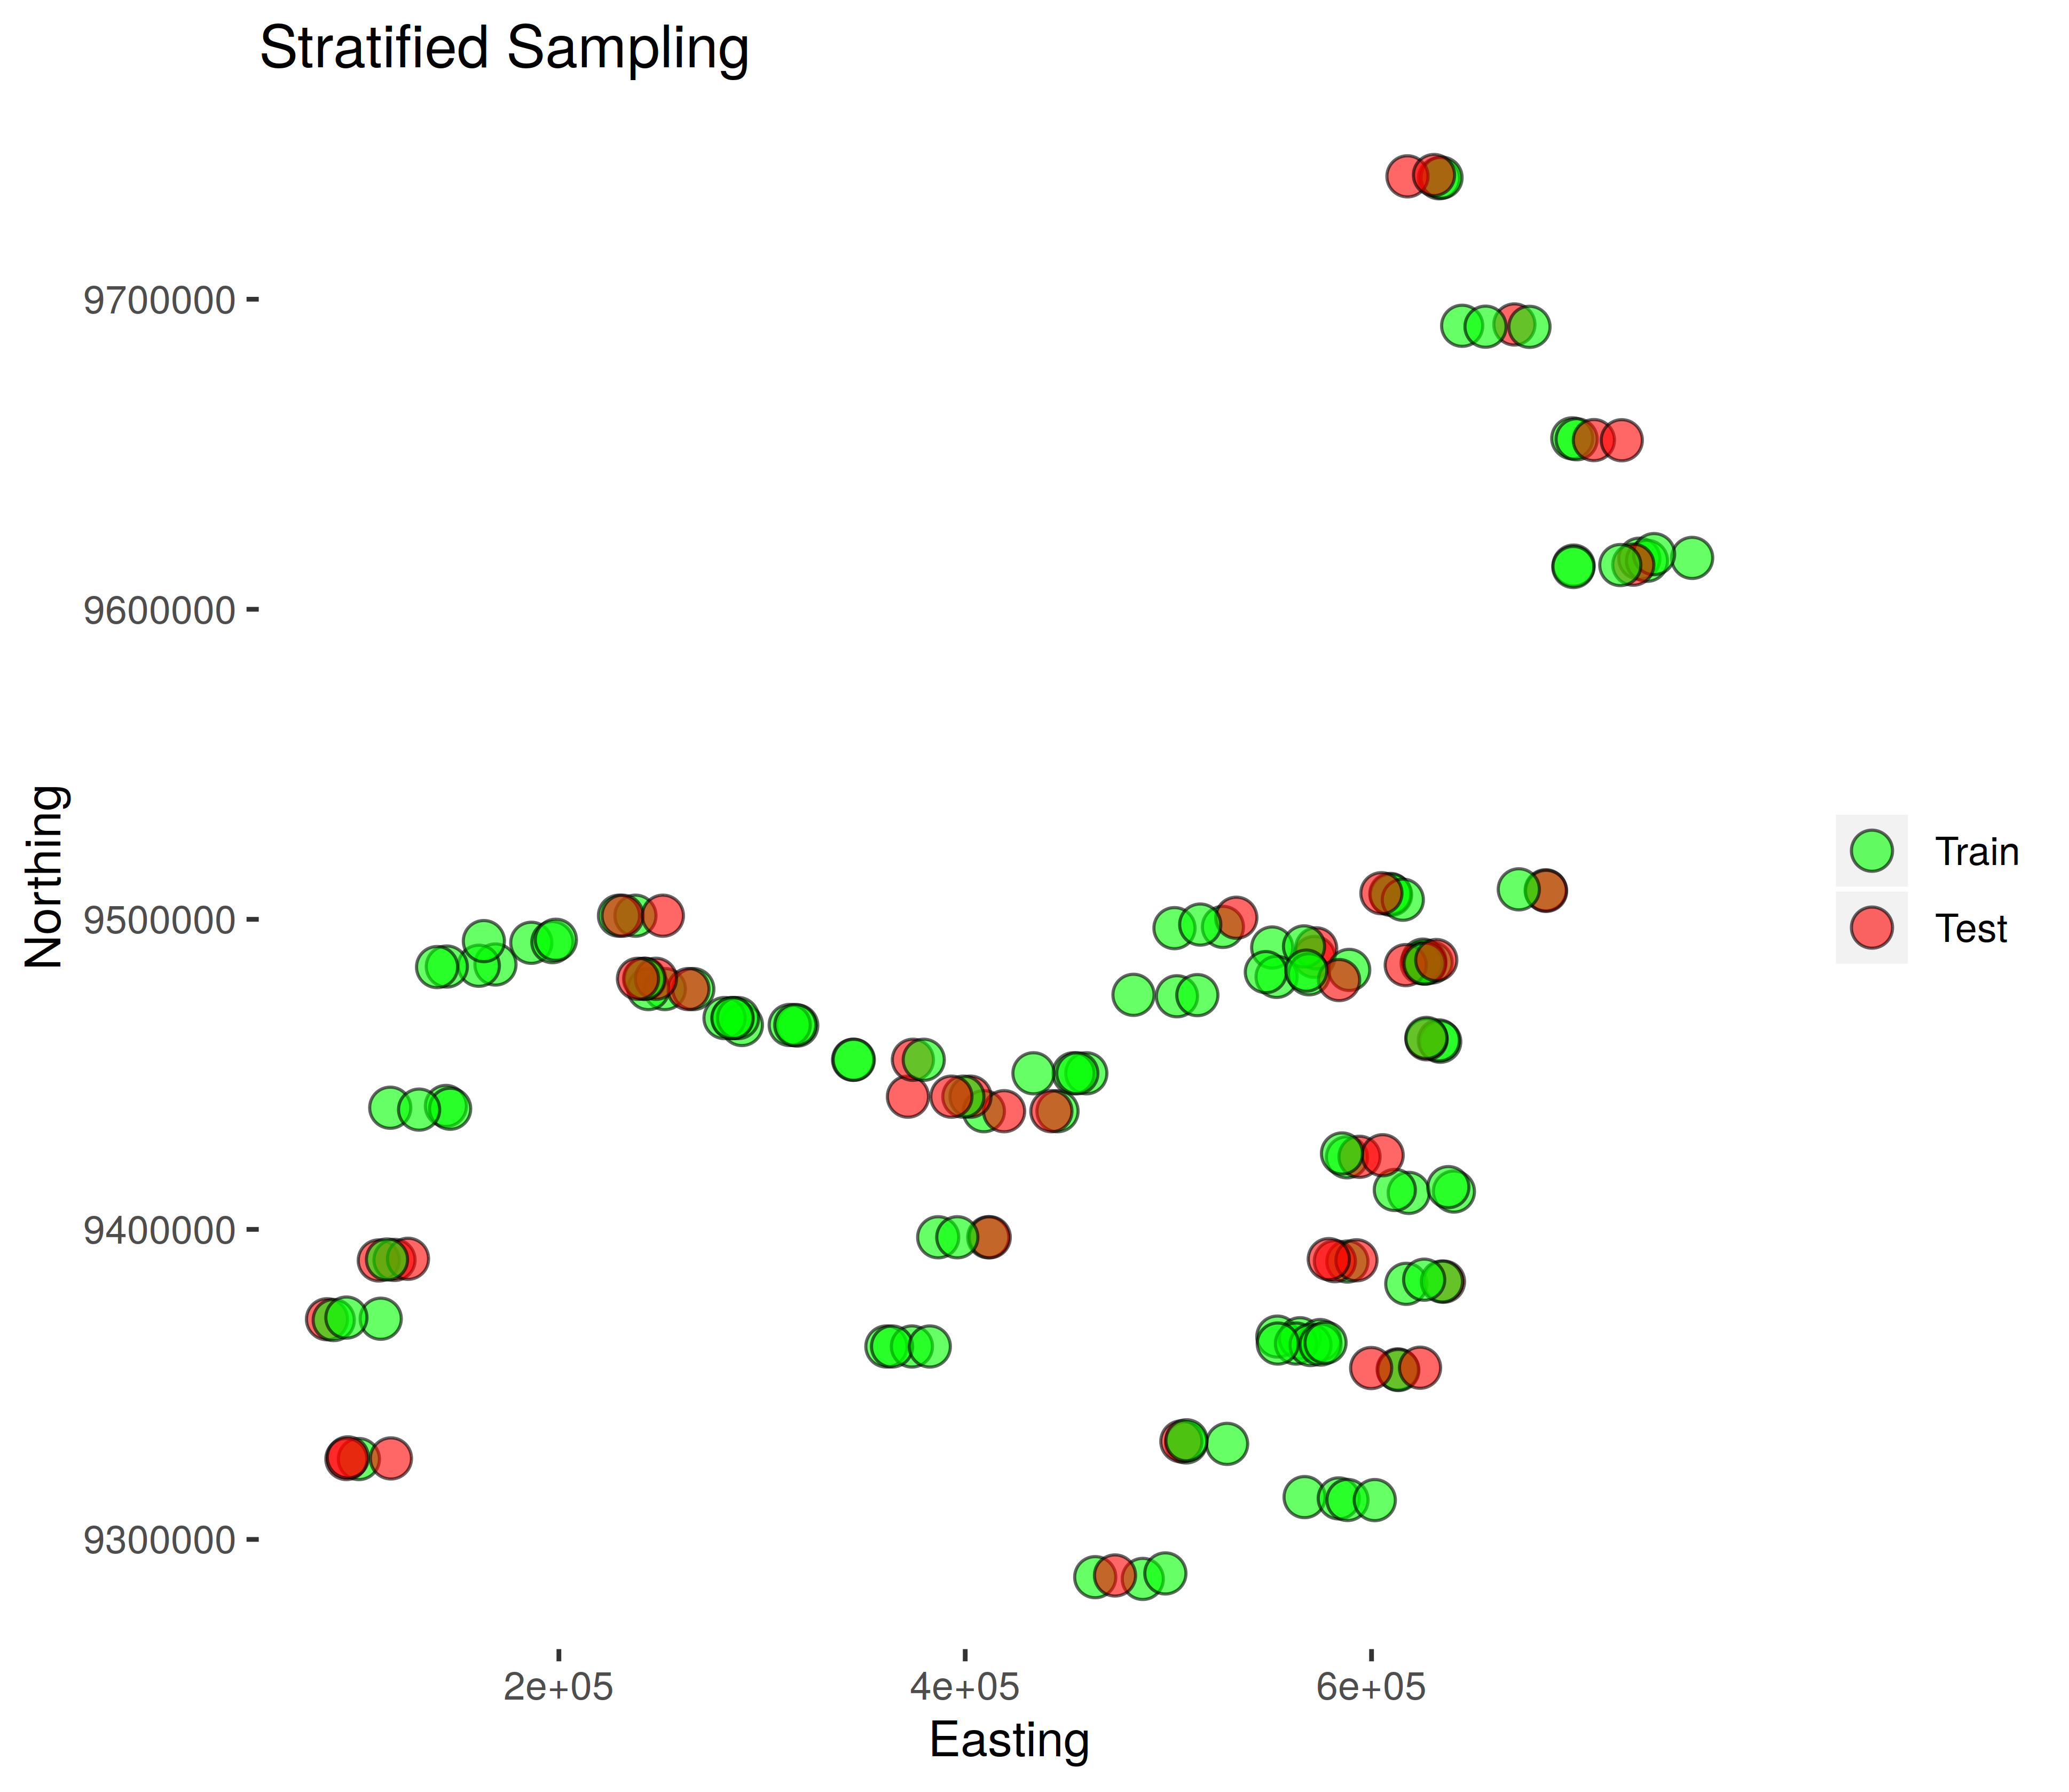
\includegraphics[width = \textwidth]{stratsamp2.png}
\end{subfigure}
\caption{Test set samples are geographically among Train set samples. This represents a maximally similar split which is created by ensuring constant distribution of samples in each part of the river in both the Train and Test set.}
\label{fig:stratsampl}
\end{figure}

%Group sample plot
\begin{figure}[h]
\centering
\begin{subfigure}{0.4\textwidth}
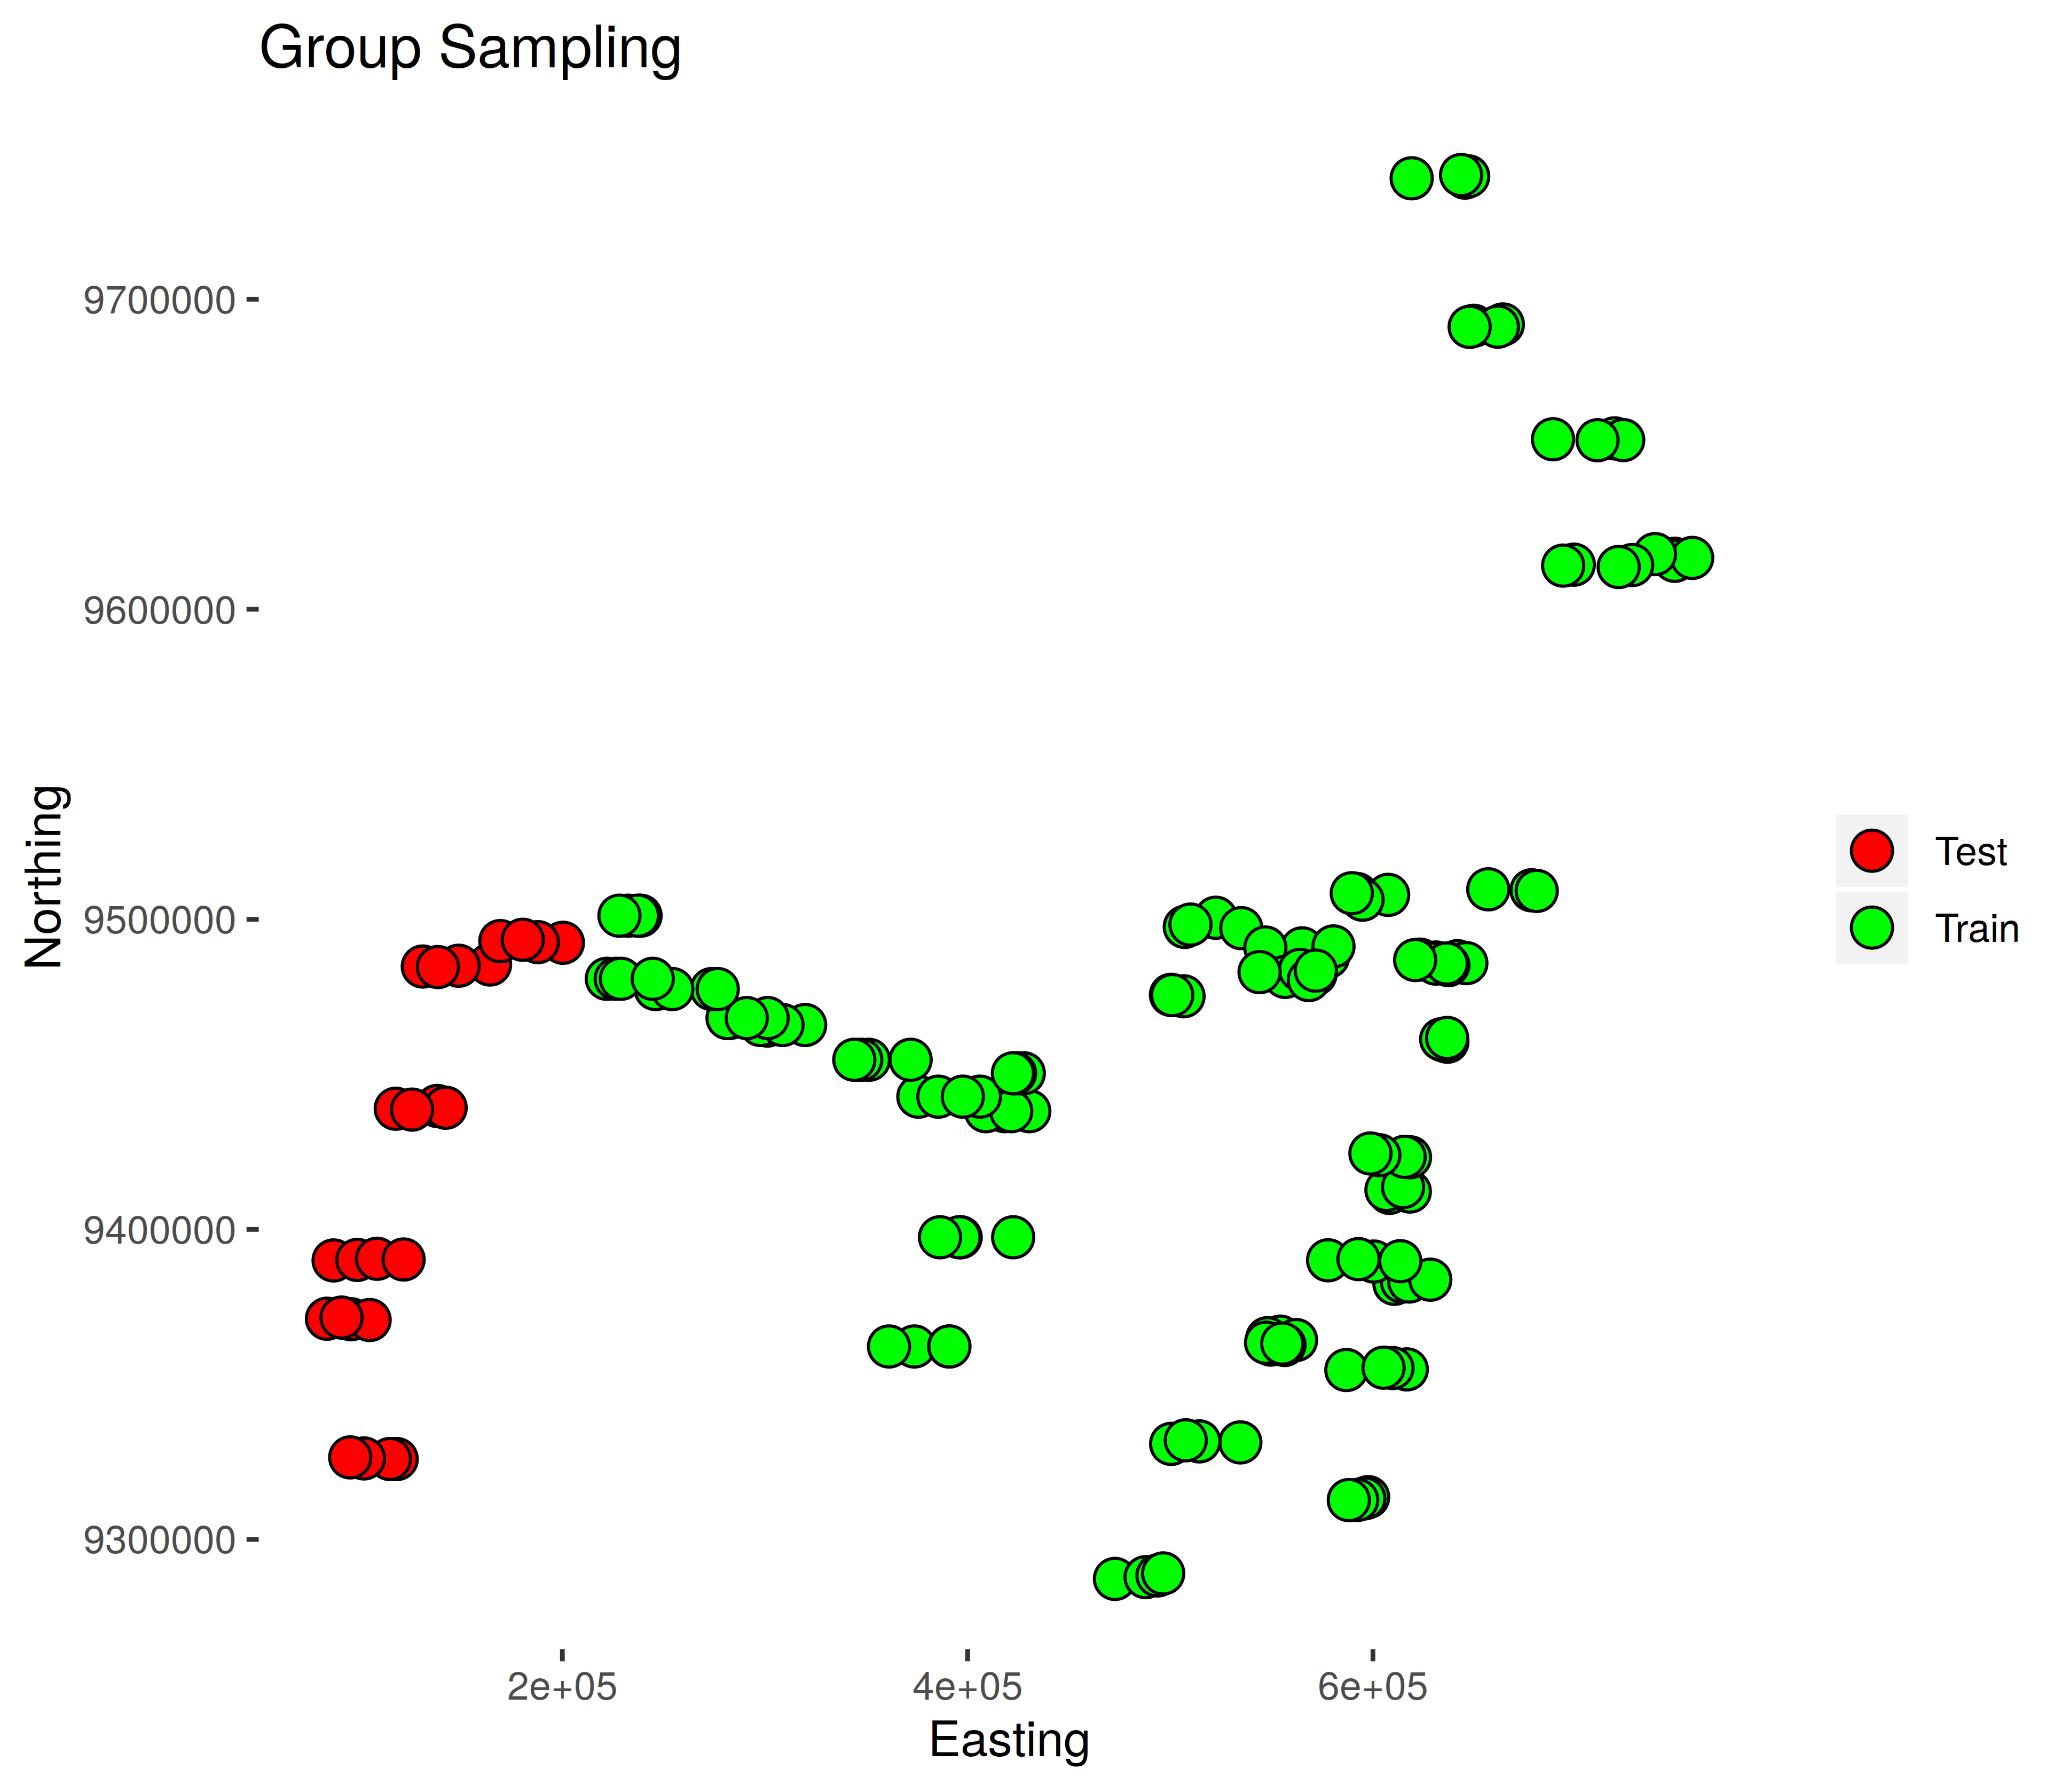
\includegraphics[width = \textwidth]{groupsamp.png}
\end{subfigure}
\begin{subfigure}{0.4\textwidth}
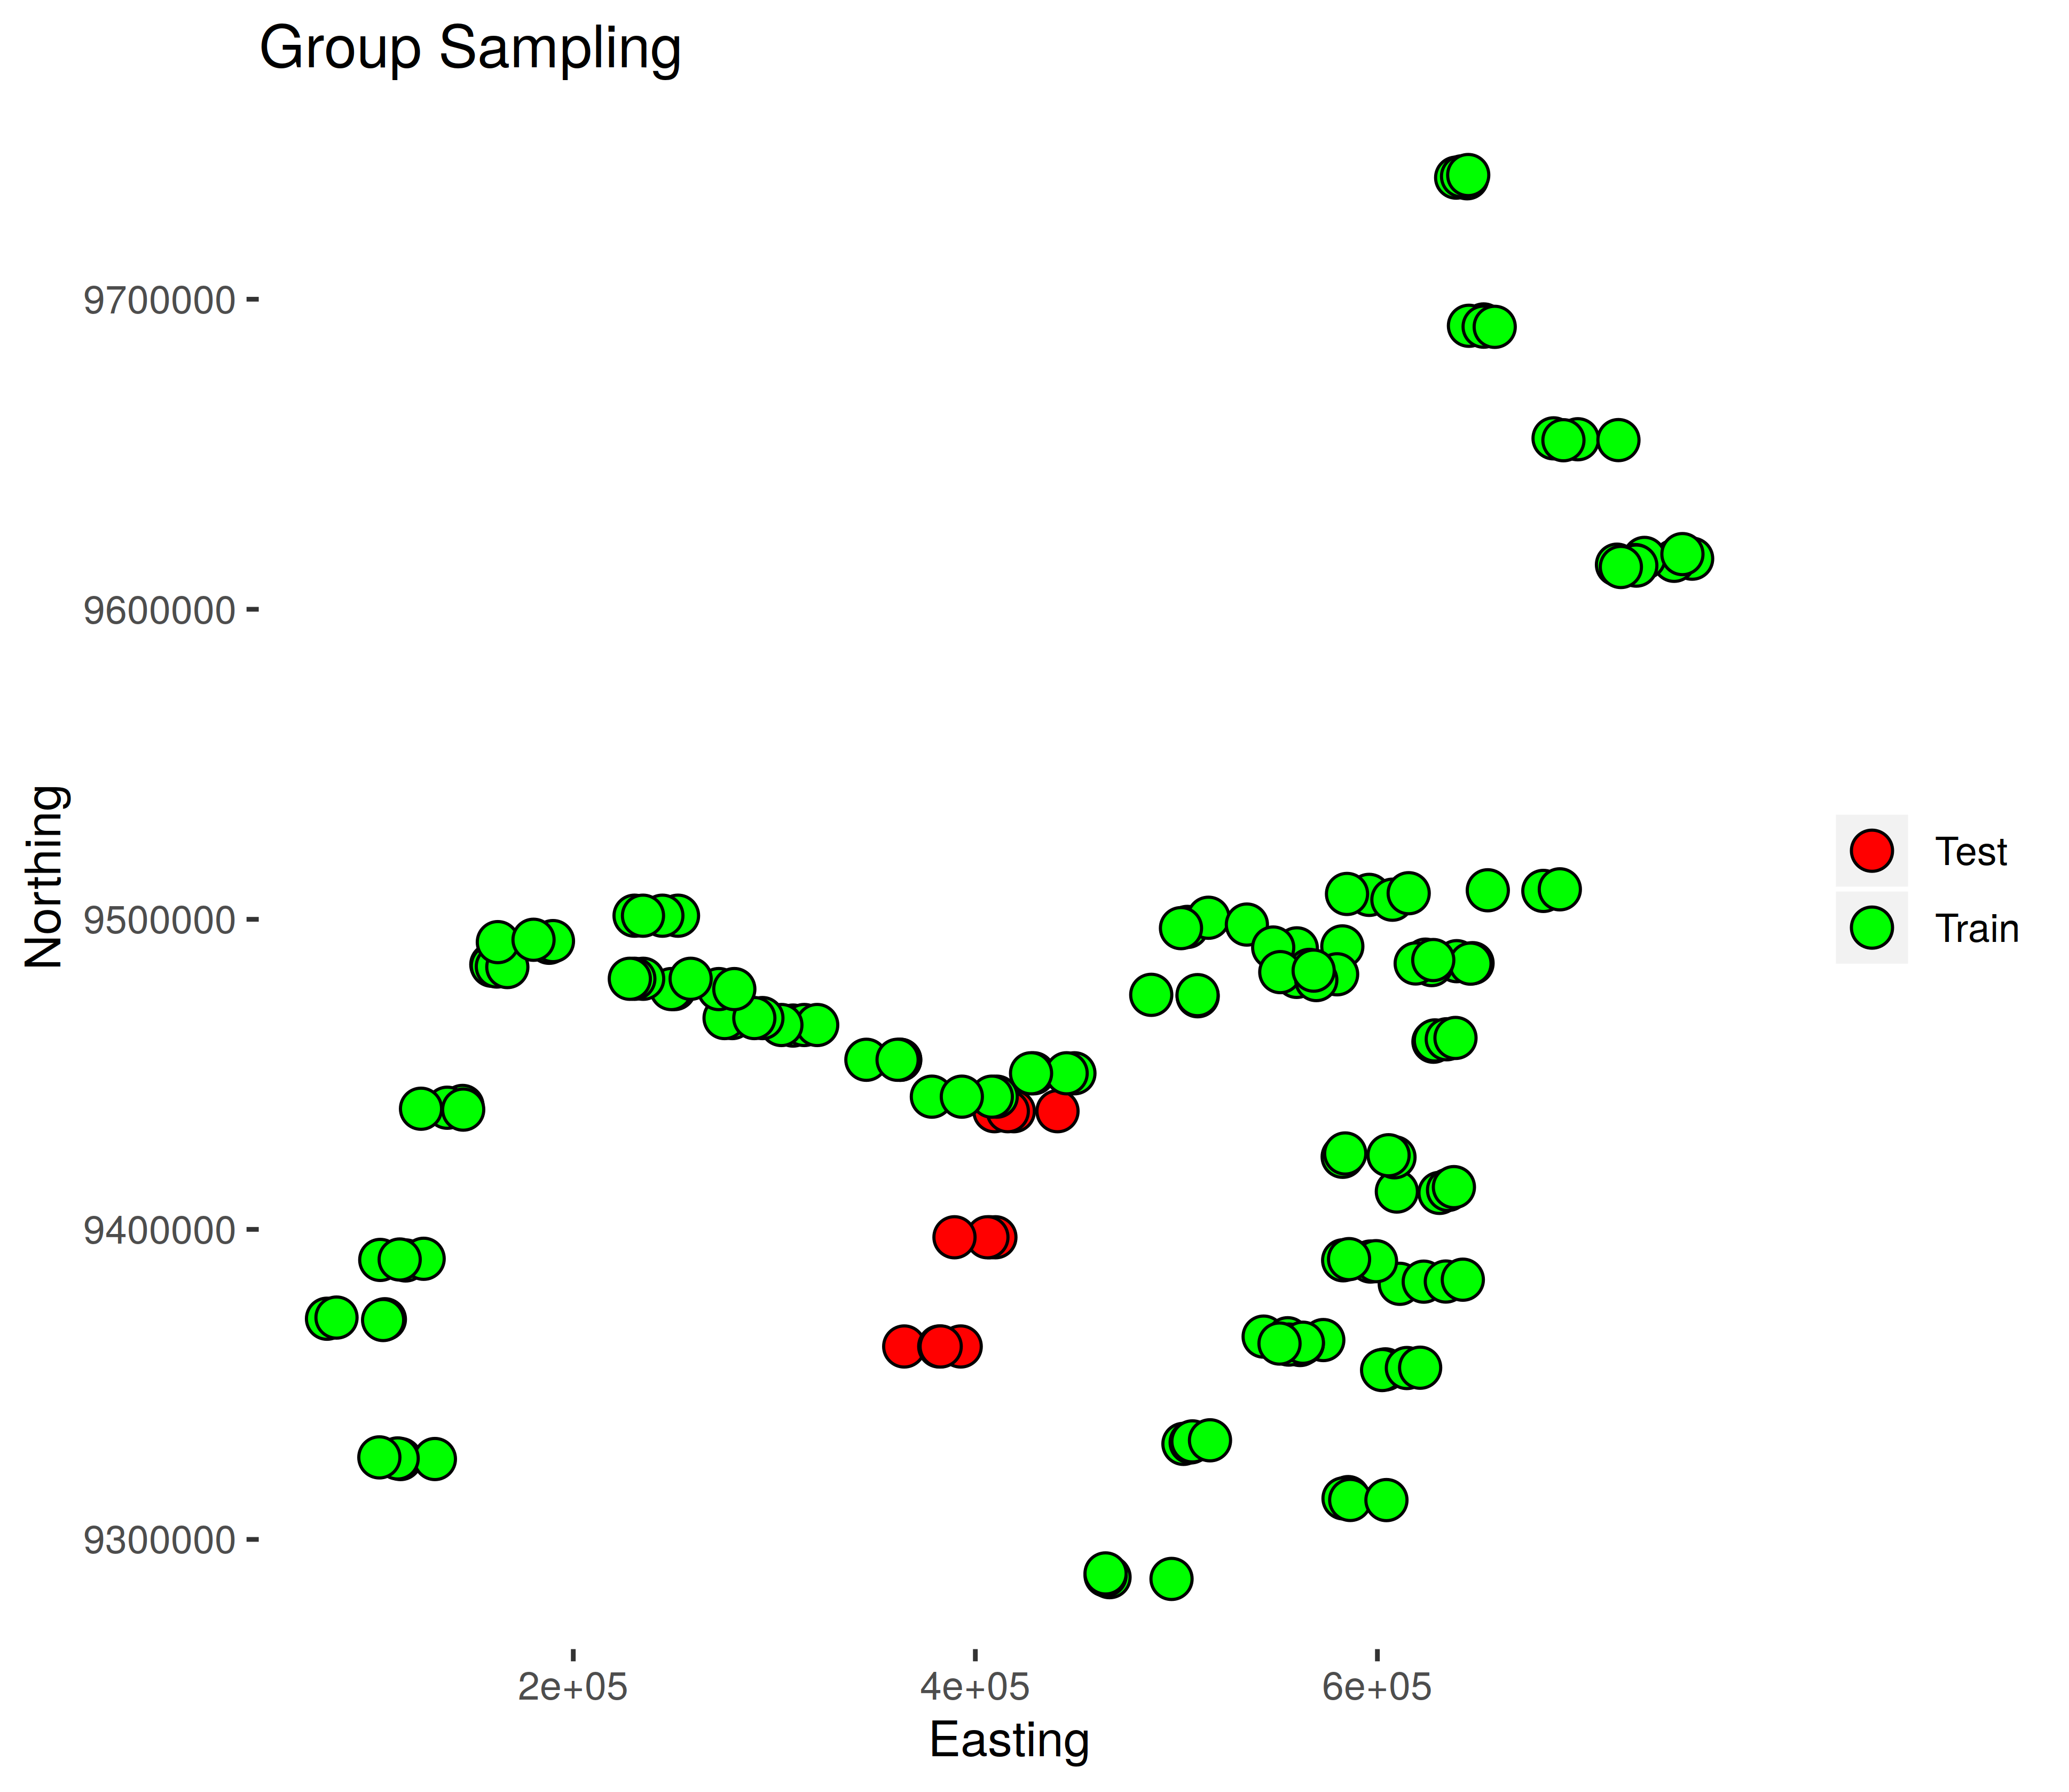
\includegraphics[width = \textwidth]{groupsamp2.png}
\end{subfigure}
\caption{Test set samples are geographically distinct from Train set samples. This represents a maximally dissimilar split which is created by choosing a different part of the river as the Testing set.}
\label{fig:groupsamp}
\end{figure}




%Validation sets
In addition to splitting the data into training and test sets, the train set was further split into validation sets so as to tune the hyperparameters of the models. The splitting into validation sets followed the same principle/method as the train-test split. So if, for example, the train and test sets were split using the maximally similar approach, the validation sets produced from the train set were chosen so as to be maximally similar to the remaining set.


The steps of testing a classifier using a specific split method are as follows:
\begin{enumerate}
\item The data set is split into train and test sets based on the splitting method of choice. 
\item The train set is split into $K$-folds using the same method for the train-test split.
\item A set of hyperparameters and potential values are chosen for the cross-validation procedure. For example, in Logistic Regression a set of numbers ranging from 0.001 to 20 is chosen for the sparsity parameter and the set $\{True,False\}$ is chosen for the intercept parameter    
\item The classifier is trained on the $K-1$ folds and tested on the remaining validation set for all possible combinations of hyperparameters (e.g. the Logistic Regressor is trained with hyperparameters $\{0.001,True\},\{0.001,False\},\{1.001,True\},\{1.001,False\}$ etc...).
\item Step 4 is repeated for all the $K$-folds (by training on the $K-1$ and testing on the one left out). The average score across the validation sets is found for each hyperparameter combination and the classifier is retrained on the train set using the best hyperparameters set.
\item The retrained model is tested on the test set and the prediction score is calculated.
\item Steps  1 through 6 are repeated a number of times for different train-test splits using the same split principles. The scores for each repetition are stored.  
\end{enumerate}

This procedure can be repeated for different features (data sets), so as to evaluate how feature selection and transformations can alter the results. The best classifier for the particular features and splitting method is the one which has the highest mean score across all train-test splits. The various data sets used to test the classifiers on are summarised in table \ref{table:features}.
\begin{table}
	\caption{Features used in Classification}
	\centering
	\label{table:features}
	\begin{tabularx}{\textwidth}{l X  }
		\hline 
		Features used &Description of dataset\\ 
		
		\hline
		OTU &The OTU table as it is without any modifications done to it \\
		OTU LOW & The OTU table without highly correlated features\\
		OTU CSS & The normalised OTU table using CSS\\
		OTU Min CSS & The normalised OTU table using CSS without samples with total counts of less than 10000 reads  \\
		OTU CSS LOG & A $\log_2$ transformed OTU CSS \\
		PCoA Bray-Curtis &The transformation of the OTU table with PCoA using the Bray-Curtis measure  \\
		PCoA Bray-Curtis CSS &The transformation of the normalised OTU table with PCoA using the Bray-Curtis measure\\
		
		\hline 
	\end{tabularx}
\end{table}

\large{\bf Maximising Similarity} \\
\textit{Aim}: Evaluate how well the classifiers perform when they are tested on a set which is similar geographically to the train set.\\
\textit{Method}: Testing and validation sets are made up of samples coming from every part of the river. Care is taken to ensure that no geographical area is over represented. This is done using Stratified sampling (using the method StratifieKfold) where the strata (or groups) are the areas of the rivers the samples belong to. Stratified sampling ensures that the distribution of test or validation samples in each area is approximately the same as for train samples.




\large{ \bf Maximising Dissimilarity}\\
\textit{Aim}: Evaluate how well the classifiers perform when they are tested on a set which is dissimilar (or far away) geographically to the train set.\\
\textit{Method}: Testing and Validation sets are made up of all the samples which belong to a particular area of the river. For example, the test set might be constituted by all the samples in the Upper Marañón area, and the validation sets by all the remaining areas (Huallaga, Min Maranon, Lower Maranon, Ucayali, Tapiche, Napo). The method used to produce these splits is called GroupKfold.

\large{\bf Random Splits}\\
\textit{Aim}: Evaluate the performance of the classifiers on train and test sets obtained by random splitting
\textit{Method}: Test and Validation sets are obtained by randomly splitting the data. Care is taken to ensure that the balance of white and black water samples is the same across splits. This is done using Stratified sampling with the colour of the river as the strata.


{\bf Ideal Splits}
An ideal sampling method would take into account the spatial correlation structures between the samples, besides just their location. Since the river flows eastwards from Maranon Upper down to all other streams, samples collected upstream would inevitably affect those from downstream, but the opposite might not be true. Thus, euclidean proximity of the river samples is not always a good enough indicator for detecting similarity between samples. For example, sample A collected near the opening of the Tapiche stream and sample B collected a bit further South of the opening, in the Ucayali stream, will have a smaller distance between them than with other samples collected further south in the Tapiche and Ucayaly streams. However, since the streams diverge, A and B might be more similar to samples found downstream their part of the river (Tapiche and Ucayaly respectively) than between them. 

To achieve this, a directed graph of the river can be constructed, with vertices representing the samples, and edges the river path between them. Then a sampling scheme can take into account the stream direction and split the dataset in more sophisticated ways. One such way can test a classifier's ability to predict river colour if the test set is downstream from the train set, and the opposite, if the test set is upstream from the train. 


%\begin{table}
%\caption{Even better looking table using booktabs}
%\centering
%\label{table:good_table}
%\begin{tabular}{l c c c c}
%\toprule
%\multirow{2}{*}{Dental measurement} & \multicolumn{2}{c}{Species I} & \multicolumn{2}{c}{Species II} \\ 
%\cmidrule{2-5}
%  & mean & SD  & mean & SD  \\ 
%\midrule
%I1MD & 6.23 & 0.91 & 5.2  & 0.7  \\
%
%I1LL & 7.48 & 0.56 & 8.7  & 0.71 \\
%
%I2MD & 3.99 & 0.63 & 4.22 & 0.54 \\
%
%I2LL & 6.81 & 0.02 & 6.66 & 0.01 \\
%
%CMD & 13.47 & 0.09 & 10.55 & 0.05 \\
%
%CBL & 11.88 & 0.05 & 13.11 & 0.04\\ 
%\bottomrule
%\end{tabular}
%\end{table}




%\include{EcologicalStats/EcoStats}
%!TEX root = ../thesis.tex
%*******************************************************************************
%****************************** Third Chapter **********************************
%*******************************************************************************
\chapter{Results}

% **************************** Define Graphics Path **************************
\ifpdf
    \graphicspath{{Chapter3/Figs/Raster/}{Chapter3/Figs/PDF/}{Chapter3/Figs/}}
\else
    \graphicspath{{Chapter3/Figs/Vector/}{Chapter3/Figs/}}
\fi

%!TEX root = ../thesis.tex
% ******************************* Thesis Appendix B ********************************

\chapter{Installing the CUED class file}

\LaTeX.cls files can be accessed system-wide when they are placed in the
<texmf>/tex/latex directory, where <texmf> is the root directory of the user’s \TeX installation. On systems that have a local texmf tree (<texmflocal>), which
may be named ``texmf-local'' or ``localtexmf'', it may be advisable to install packages in <texmflocal>, rather than <texmf> as the contents of the former, unlike that of the latter, are preserved after the \LaTeX system is reinstalled and/or upgraded.

It is recommended that the user create a subdirectory <texmf>/tex/latex/CUED for all CUED related \LaTeX class and package files. On some \LaTeX systems, the directory look-up tables will need to be refreshed after making additions or deletions to the system files. For \TeX Live systems this is accomplished via executing ``texhash'' as root. MIK\TeX users can run ``initexmf -u'' to accomplish the same thing.

Users not willing or able to install the files system-wide can install them in their personal directories, but will then have to provide the path (full or relative) in addition to the filename when referring to them in \LaTeX.
%\include{Chapter5/chapter5}
%\include{Chapter6/chapter6}
%\include{Chapter7/chapter7}



% ********************************** Back Matter *******************************
% Backmatter should be commented out, if you are using appendices after References
%\backmatter

% ********************************** Bibliography ******************************
\begin{spacing}{0.9}

% To use the conventional natbib style referencing
% Bibliography style previews: http://nodonn.tipido.net/bibstyle.php
% Reference styles: http://sites.stat.psu.edu/~surajit/present/bib.htm

%\bibliographystyle{apalike}
%%\bibliographystyle{unsrt} % Use for unsorted references  
%%\bibliographystyle{plainnat} % use this to have URLs listed in References
%\cleardoublepage
%\bibliography{References/references} % Path to your References.bib file


% If you would like to use BibLaTeX for your references, pass `custombib' as
% an option in the document class. The location of 'reference.bib' should be
% specified in the preamble.tex file in the custombib section.
% Comment out the lines related to natbib above and uncomment the following line.

\printbibliography[heading=bibintoc, title={References}]


\end{spacing}

% ********************************** Appendices ********************************

\begin{appendices} % Using appendices environment for more functunality

%!TEX root = ../thesis.tex
% ******************************* Thesis Appendix A ****************************
\chapter{Appendix} 
\ifpdf
\graphicspath{{Chapter3/Figs/Raster/}{Chapter3/Figs/PDF/}{Chapter3/Figs/}}
\else
\graphicspath{{Chapter3/Figs/Vector/}{Chapter3/Figs/}}
\fi
Here we present additional results for different features sets than the ones presented in Chapter \ref{chap:results}, so as to complete and complement the discussion without burdening the reader with long, difficult to read tables and figures.

The PCoA sets presented here were computed using the Bray-Curtis distance measure; their only difference with the ones presented in the Results \& Discussion Chapter is that only some of the axes where used for classification. In particular, the first axes to describe 99\% and 90\% of the variance were used. Also, the configuration of a 20-dimensional NMDS ordination was used as a feature set. The procedure was run for 10000 steps and did not converge, so it does not represent the best 20-dimensional NMDS configuration.


The results for maximum similarity are presented in tables \ref{table:lrsimilarityappendix} for Logistic regression and \ref{table:rfrsimilarityappendix} for Random Forest. As with the other feature sets, Logistic regression is outperforming Random Forest (except for NMDS). Both methods are above the baseline.
%SIMILARITY
%SIM LOG 
\begin{table}[h]
	\centering
	\begin{tabular}{l c  c c}
		\toprule
		&\multicolumn{2}{c}{Confusion Matrix} & Accuracy\\
		Features used & Predicted Black&Predicted White&\\
		\midrule
		\multirow{2}{*}{PCoA 99\%} &16 &5&\multirow{2}{*}{95.12\%}\\
		&	 3&140&\\
		\cmidrule{2-3}
		\multirow{2}{*}{PCoA 90\%} &16 &5&\multirow{2}{*}{95.12\%}\\
		&	 3&140&\\
		\cmidrule{2-3}
		\multirow{2}{*}{PCoA CSS 99\%} &16 &5&\multirow{2}{*}{96.34\%}\\
		&	 1&142&\\
		\cmidrule{2-3}
		\multirow{2}{*}{PCoA CSS 90\%} &16 &5&\multirow{2}{*}{95.73\%}\\
		&	 2&141&\\
		\cmidrule{2-3}
		\multirow{2}{*}{NMDS}&13 &8&\multirow{2}{*}{90.24\%}\\
		&	 8&135&\\
				\cmidrule{2-3}
		\multirow{2}{*}{PCA}&4 &17&\multirow{2}{*}{88.41\%}\\
		&	 2&141&\\
		\bottomrule
	\end{tabular}
	\caption{Results from maximising similarity using Logistic Regression. The percentages indicate the total variance the axes of PCoA explain.}
	\label{table:lrsimilarityappendix}
\end{table}

%RFR SIMILARITY
\begin{table}[h]
	\centering
	\begin{tabular}{l c  c c}
		\toprule
		&\multicolumn{2}{c}{Confusion Matrix} & Accuracy\\
		Features used & Predicted Black&Predicted White&\\
		\midrule
		\multirow{2}{*}{PCoA 99\%} &4 &17&\multirow{2}{*}{86.59\%}\\
		&	 5&138&\\
		\cmidrule{2-3}
		\multirow{2}{*}{PCoA 90\%} &9 &12&\multirow{2}{*}{90.24\%}\\
		&	 4&139&\\
		\cmidrule{2-3}
		\multirow{2}{*}{PCoA CSS 99\%} &10 &11&\multirow{2}{*}{93.29\%}\\
		&	 0&143&\\
		\cmidrule{2-3}
		\multirow{2}{*}{PCoA CSS 90\%} &12 &9&\multirow{2}{*}{94.51\%}\\
		&	 0&143&\\
		\cmidrule{2-3}
		\multirow{2}{*}{NMDS}&10 &11&\multirow{2}{*}{92.07\%}\\
		&	 2&141&\\
						\cmidrule{2-3}
		\multirow{2}{*}{PCA}&2 &19&\multirow{2}{*}{88.41\%}\\
		&	 0&143&\\
		\bottomrule
	\end{tabular}
	\caption{Results from maximising similarity using Random Forest. The percentages indicate the total variance the axes of PCoA explain.}
	\label{table:rfrsimilarityappendix}
\end{table}
%PIE SIMILARITY






%DISSIMILARITY
The results for maximum dissimilarity are presented in tables \ref{table:lrdissimilarityappendix} for Logistic regression and \ref{table:rfrdissimilarityappendix} for Random Forest. Unlike the other feature sets in the same setting, Logistic regression is outperforming Random Forest (except for NMDS). Both methods are above the baseline. It is interesting to note that the sets PCoA 90\% and PCoA CSS 99\% produce a better accuracy for Logistic regression than its best set in Chapter \ref{chap:results}. 
%LOG DISSIM
\begin{table}[h]
	\centering
	\begin{tabular}{l c  c c}
		\toprule
		&\multicolumn{2}{c}{Confusion Matrix} & Accuracy\\
		Features used & Predicted Black&Predicted White&\\
		\midrule
		\multirow{2}{*}{PCoA 99\%} &7 &14&\multirow{2}{*}{86.59\%\%}\\
		&	 8&135&\\
		\cmidrule{2-3}
		\multirow{2}{*}{PCoA 90\%} &7 &14&\multirow{2}{*}{88.41\%}\\
		&	 5&138&\\
		\cmidrule{2-3}
		\multirow{2}{*}{PCoA CSS 99\%} &8 &13&\multirow{2}{*}{89.02\%}\\
		&	 5&138&\\
		\cmidrule{2-3}
		\multirow{2}{*}{PCoA CSS 90\%} &8 &13&\multirow{2}{*}{85.37\%}\\
		&	11&132&\\
		\cmidrule{2-3}
		\multirow{2}{*}{NMDS}&3 &18&\multirow{2}{*}{82.93\%}\\
		&	 10&133&\\
						\cmidrule{2-3}
		\multirow{2}{*}{PCA}&0 &21&\multirow{2}{*}{87.20\%}\\
		&	 0&143&\\
		\bottomrule
	\end{tabular}
	\caption{Results from maximising dissimilarity using Logistic Regression. The percentages indicate the total variance the axes of PCoA explain.}
	\label{table:lrdissimilarityappendix}
\end{table}

%RFR DISSIM
\begin{table}[h]
	\centering
	\begin{tabular}{l c  c c}
		\toprule
		&\multicolumn{2}{c}{Confusion Matrix} & Accuracy\\
		Features used & Predicted Black&Predicted White&\\
		\midrule
		\multirow{2}{*}{PCoA 99\%} &0 &21&\multirow{2}{*}{84.76\%}\\
		&	4&139&\\
		\cmidrule{2-3}
		\multirow{2}{*}{PCoA 90\%}  &0 &21&\multirow{2}{*}{84.76\%}\\
		&	4&139&\\
		\cmidrule{2-3}
		\multirow{2}{*}{PCoA CSS 99\%}  &0 &21&\multirow{2}{*}{84.76\%}\\
		&	4&139&\\
		\cmidrule{2-3}
		\multirow{2}{*}{PCoA CSS 90\%} &0 &21&\multirow{2}{*}{84.15\%}\\
		&	5&138&\\
		\cmidrule{2-3}
		\multirow{2}{*}{NMDS}&1 &20&\multirow{2}{*}{86.59\%}\\
		&	 2&141&\\
						\cmidrule{2-3}
		\multirow{2}{*}{PCA}&0 &21&\multirow{2}{*}{81.71\%}\\
		&	 9&134&\\
		\bottomrule
	\end{tabular}
	\caption{Results from maximising dissimilarity using Random Forest. The percentages indicate the total variance the axes of PCoA explain.}
	\label{table:rfrdissimilarityappendix}
\end{table}
%PIE DISSIM

We used the feature importance method of Random Forest to determine which taxonomic Orders contribute the most to the predictive power of the classifier. Figure \ref{fig:dispieappendix} shows the mean and sum aggregation for the OTU and OTU MIN CSS feature sets in the maximum similarity setting. Figure \ref{fig:simpieappendix} for the maximum dissimilarity.

\begin{figure}[h]
	\centering
	\begin{subfigure}{0.45\textwidth}
		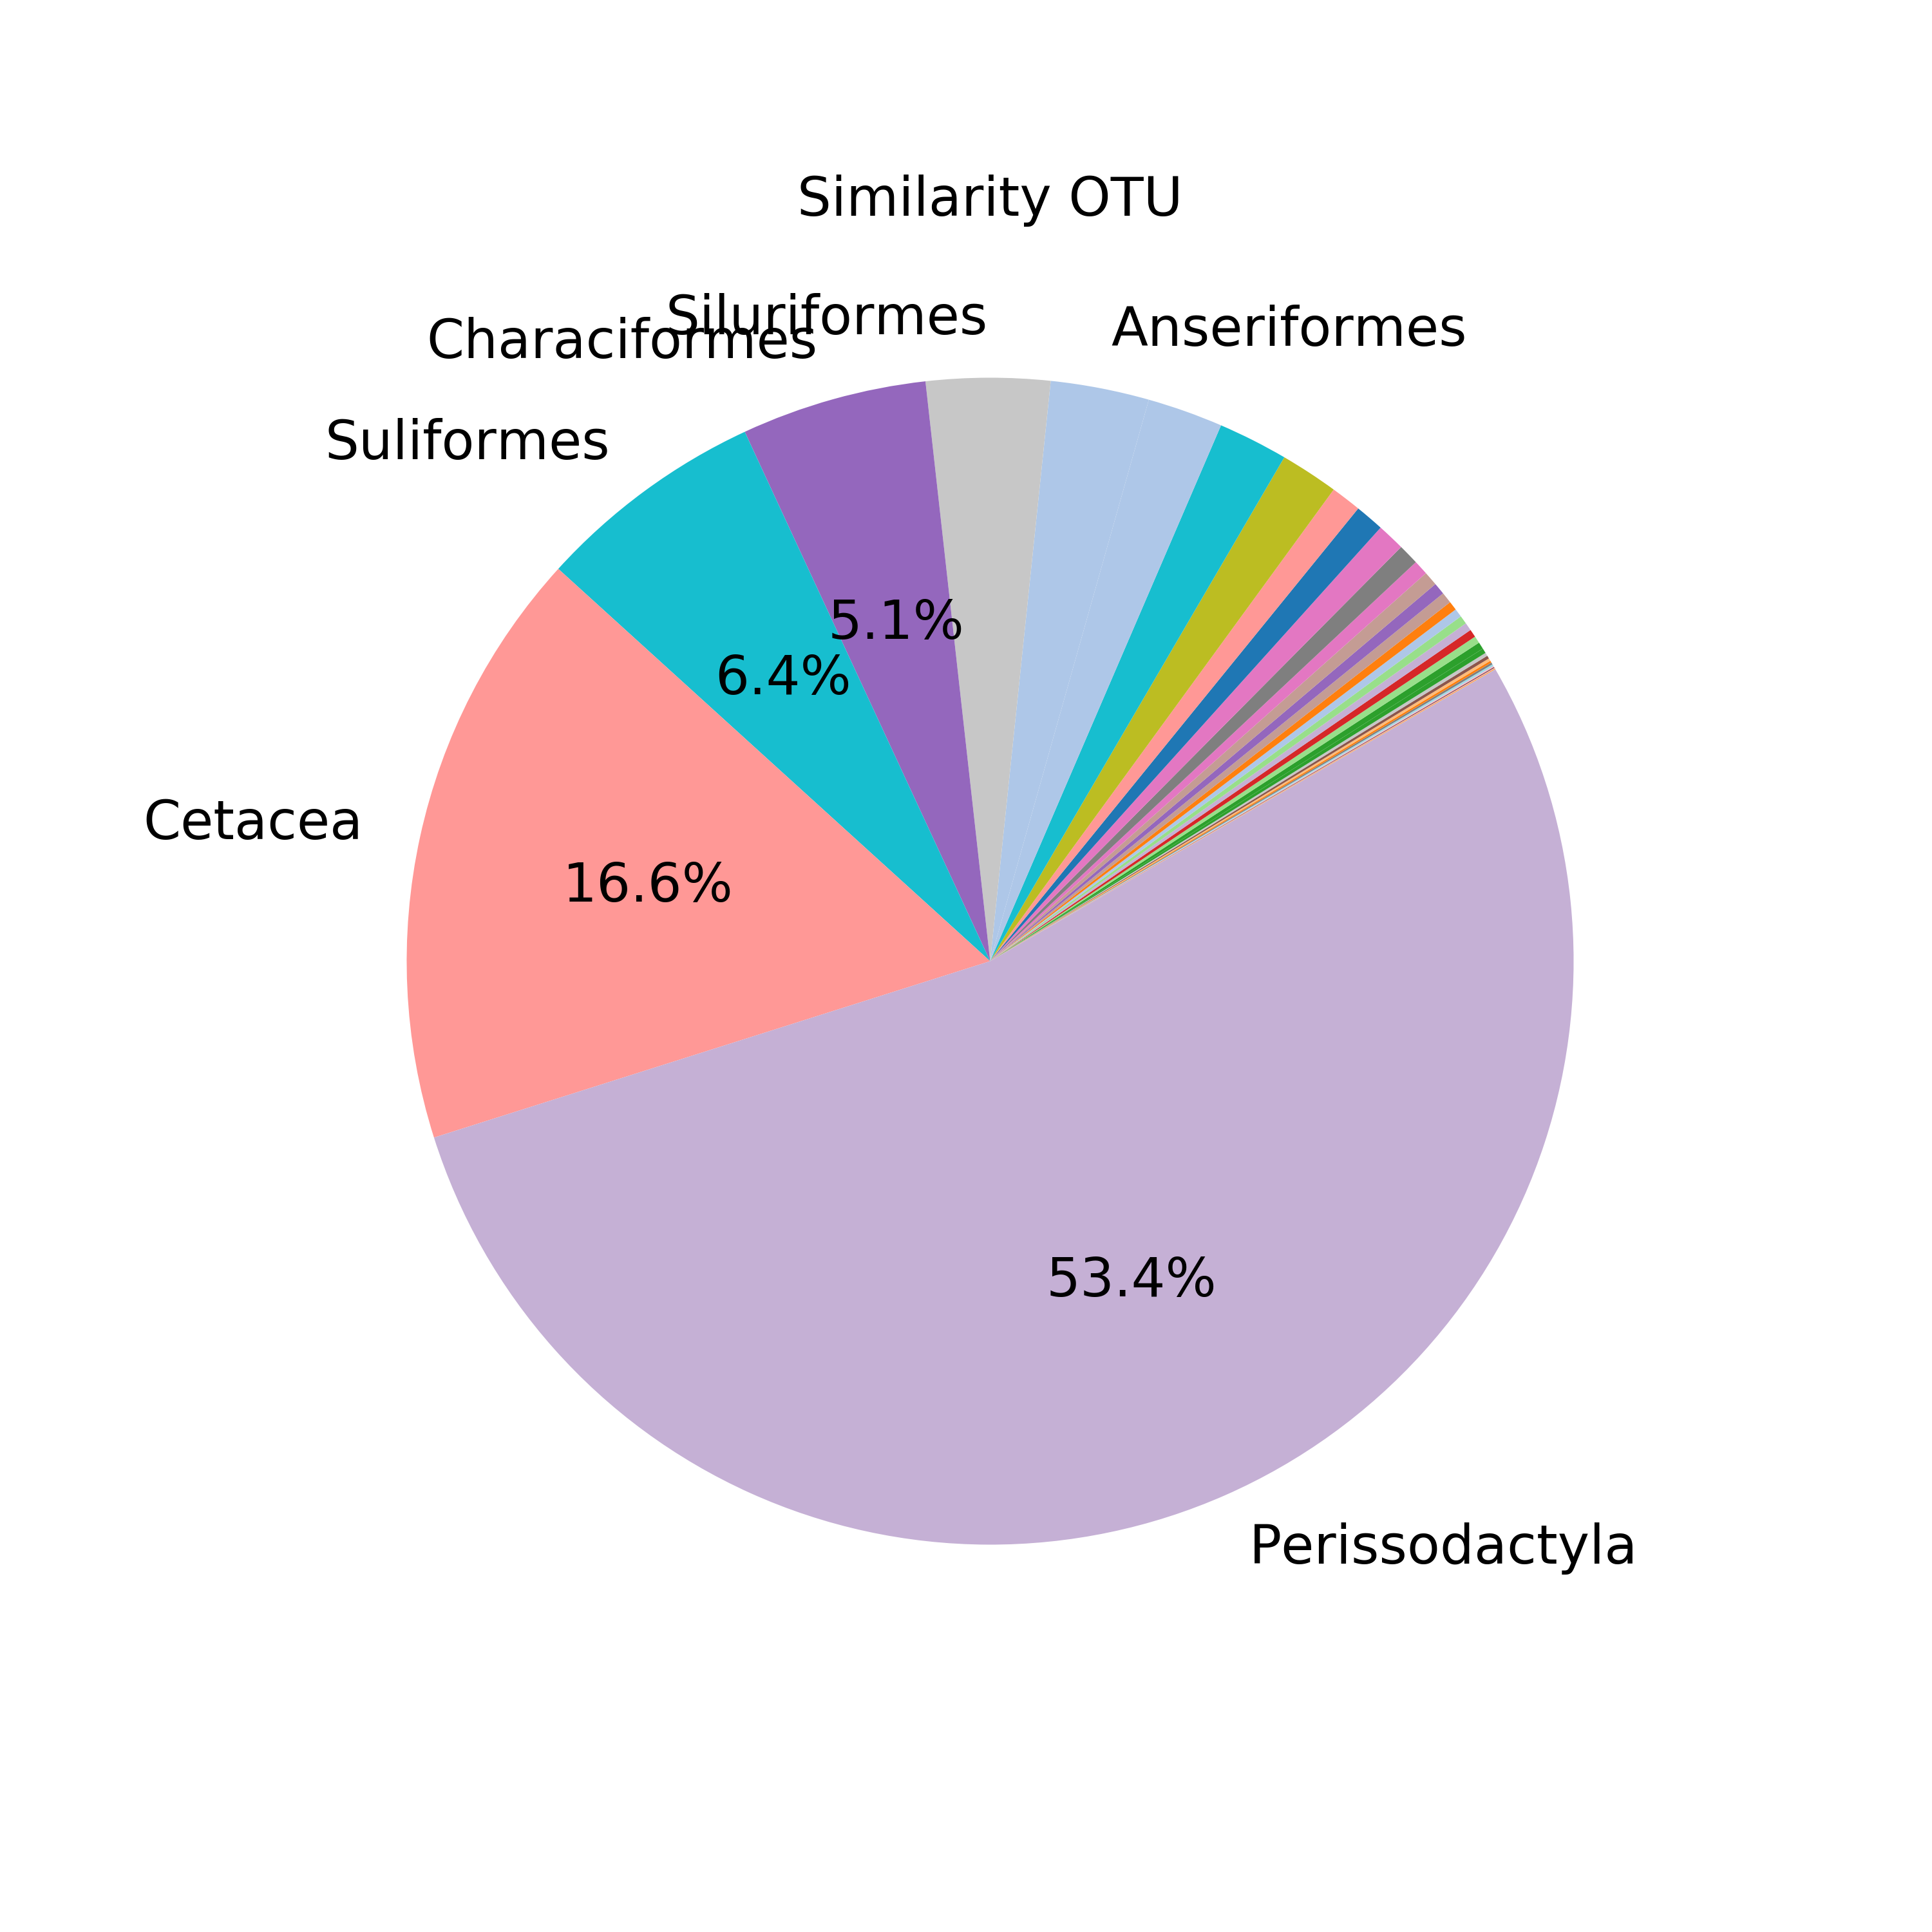
\includegraphics[width=\textwidth]{rfr_sim_mean_pieOTU}
		\caption{}
		\label{fig:simotumean}
	\end{subfigure}
	\begin{subfigure}{0.45\textwidth}
		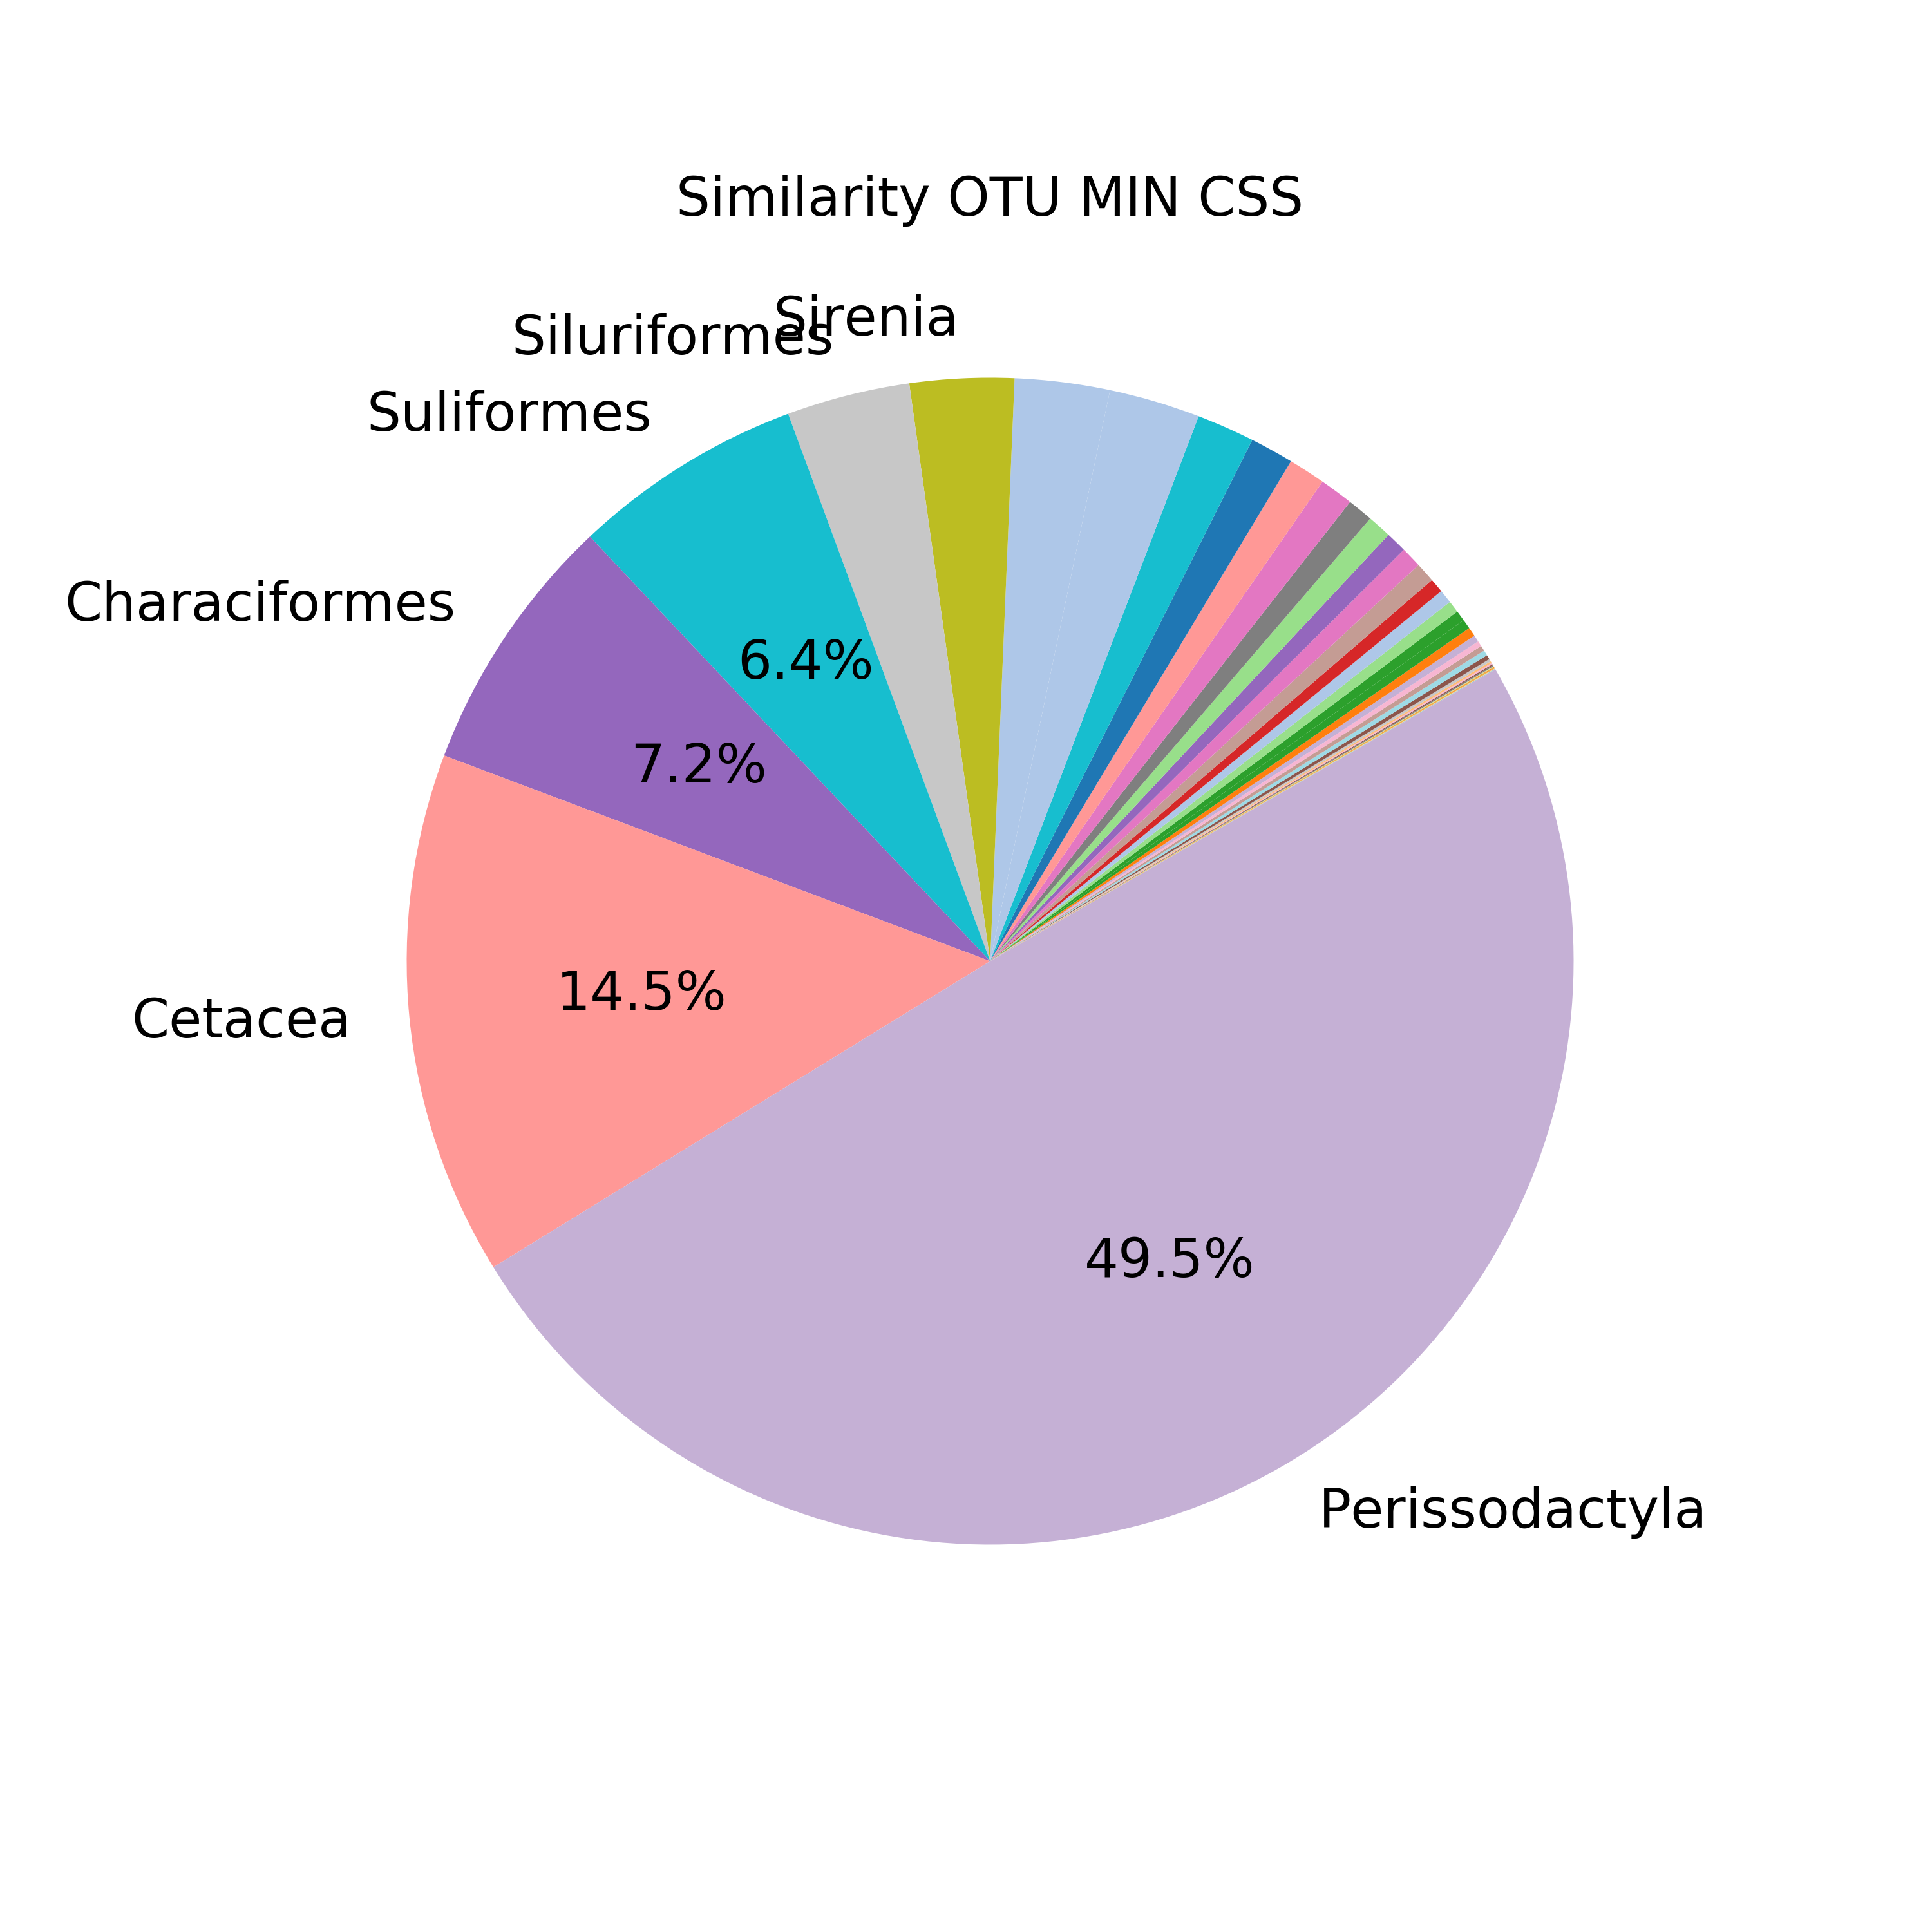
\includegraphics[width=\textwidth]{rfr_sim_mean_pieOTU MIN CSS}
		\caption{}
		\label{fig:simotumincssmean}
	\end{subfigure}\\
	\begin{subfigure}{0.45\textwidth}
		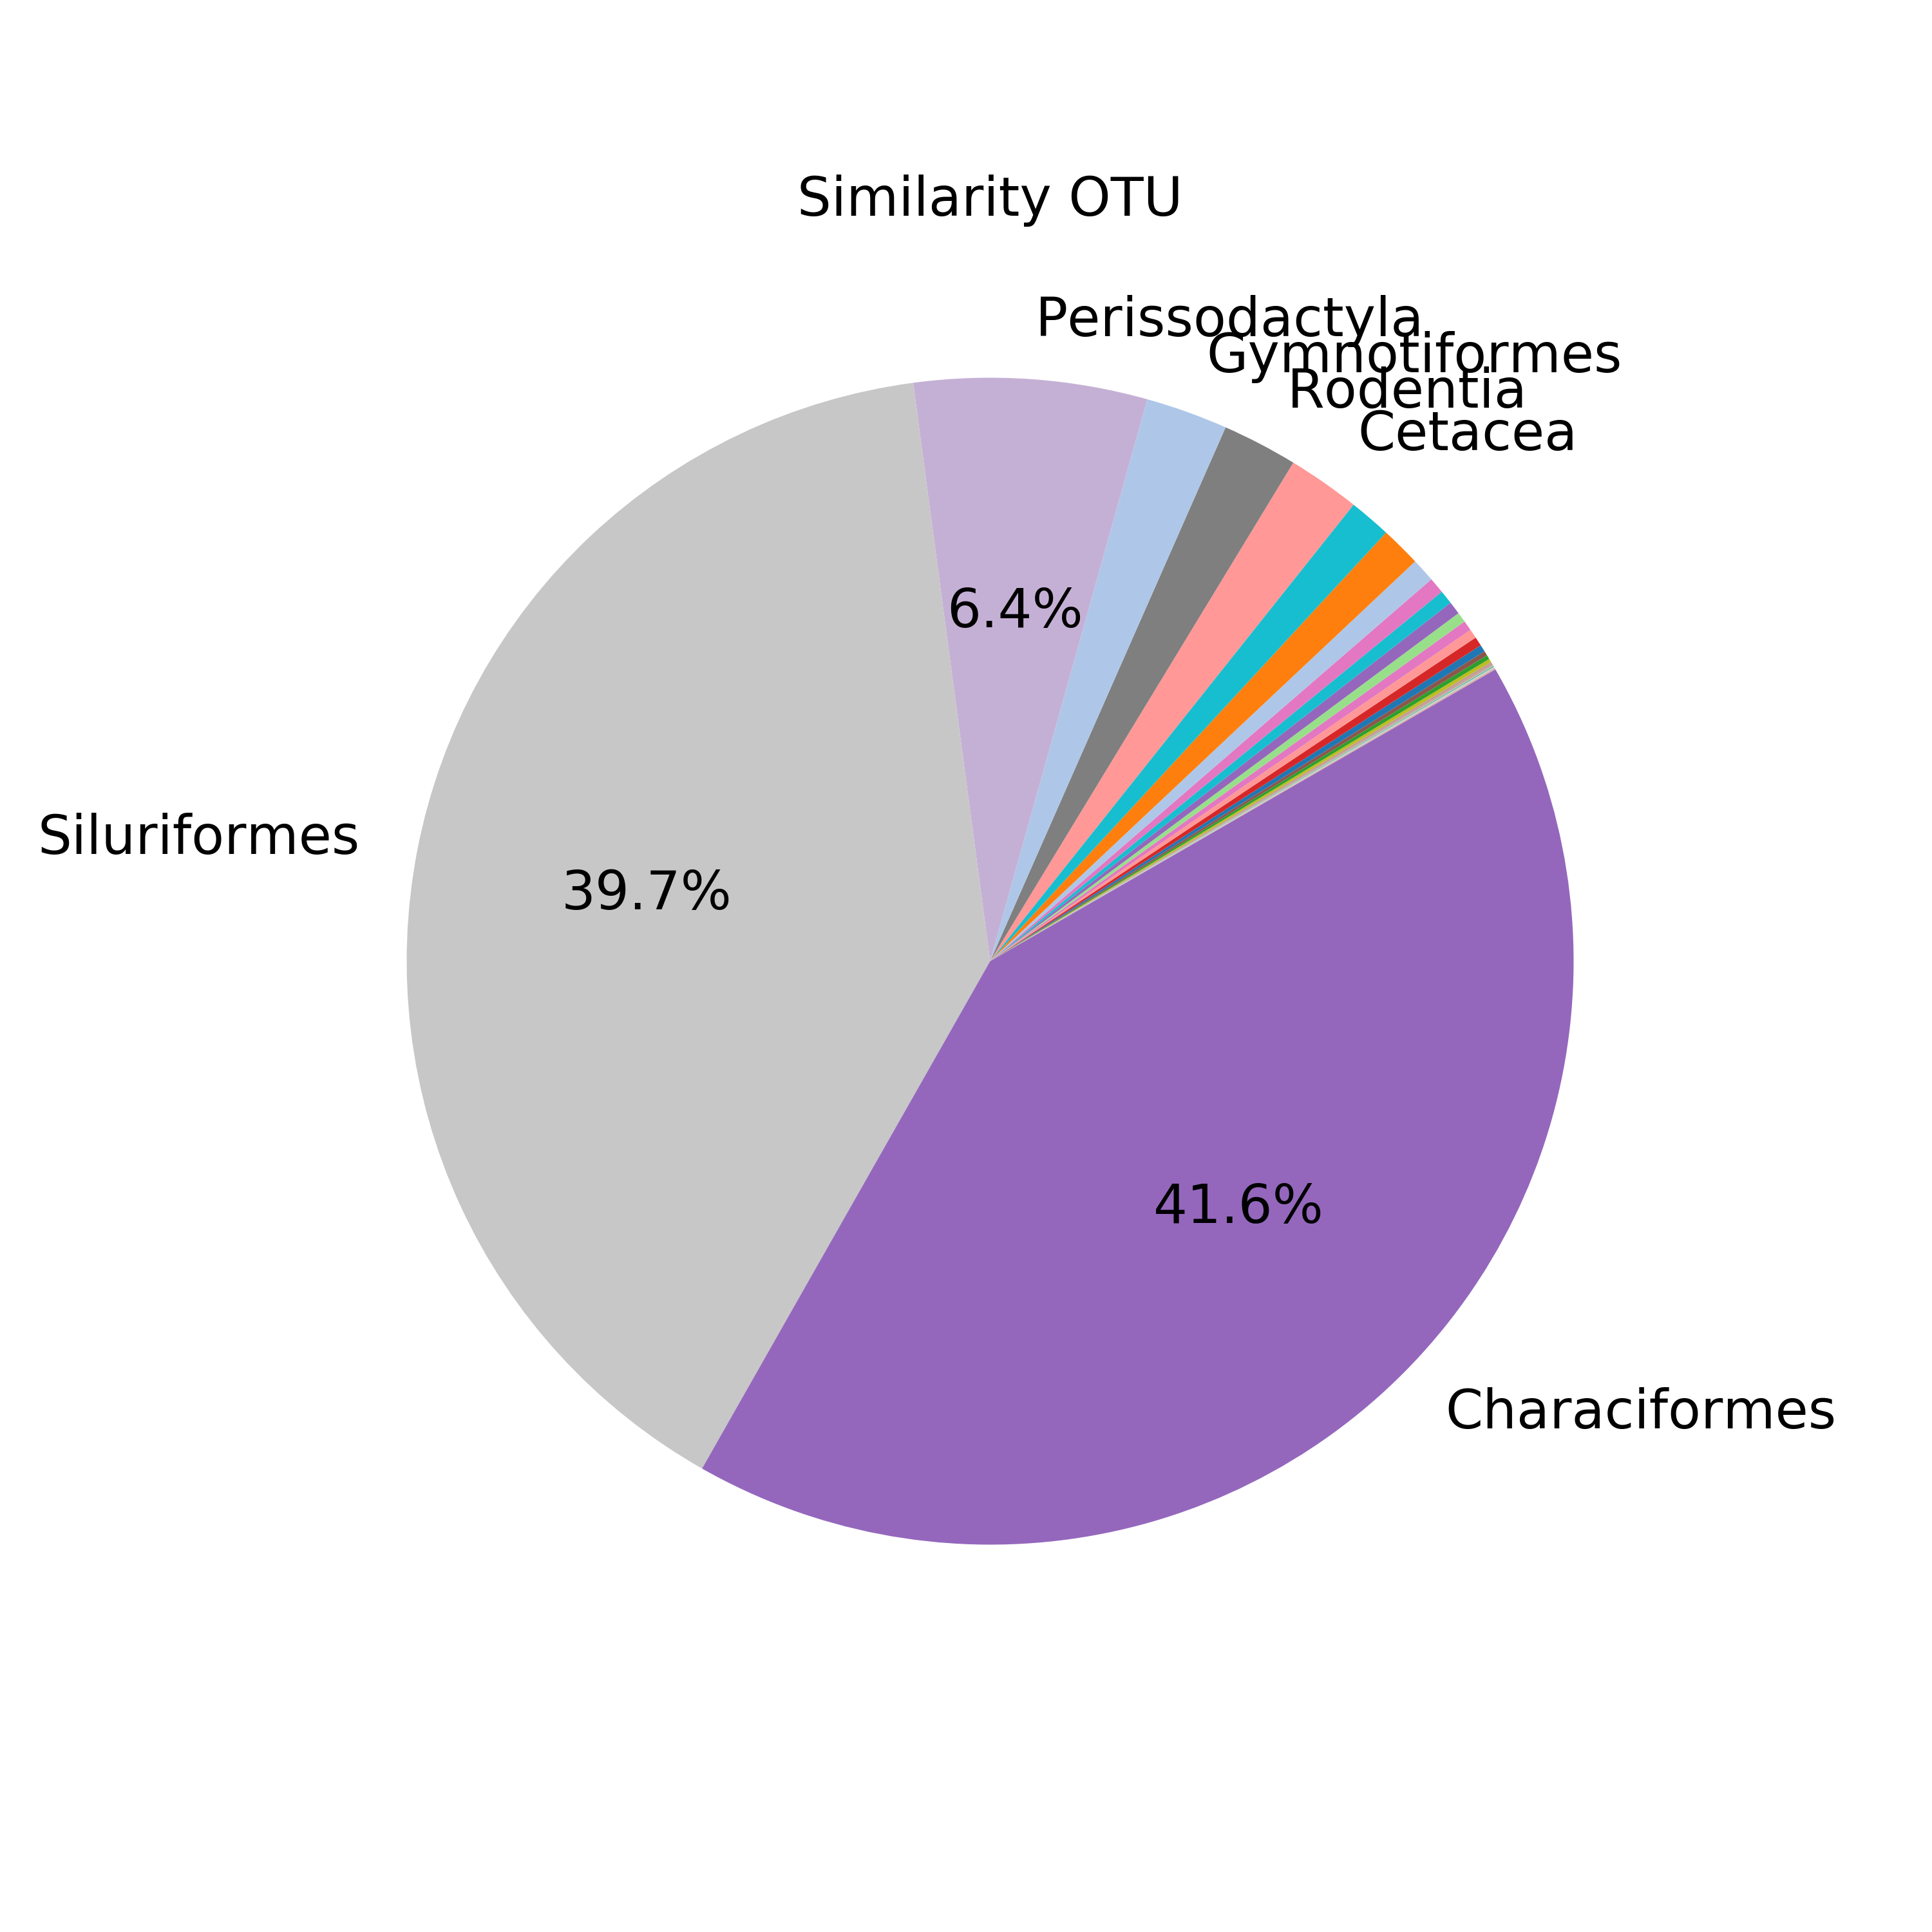
\includegraphics[width=\textwidth]{rfr_sim_sum_pieOTU}
		\caption{}
		\label{fig:simotusum}
	\end{subfigure}
	\begin{subfigure}{0.45\textwidth}
		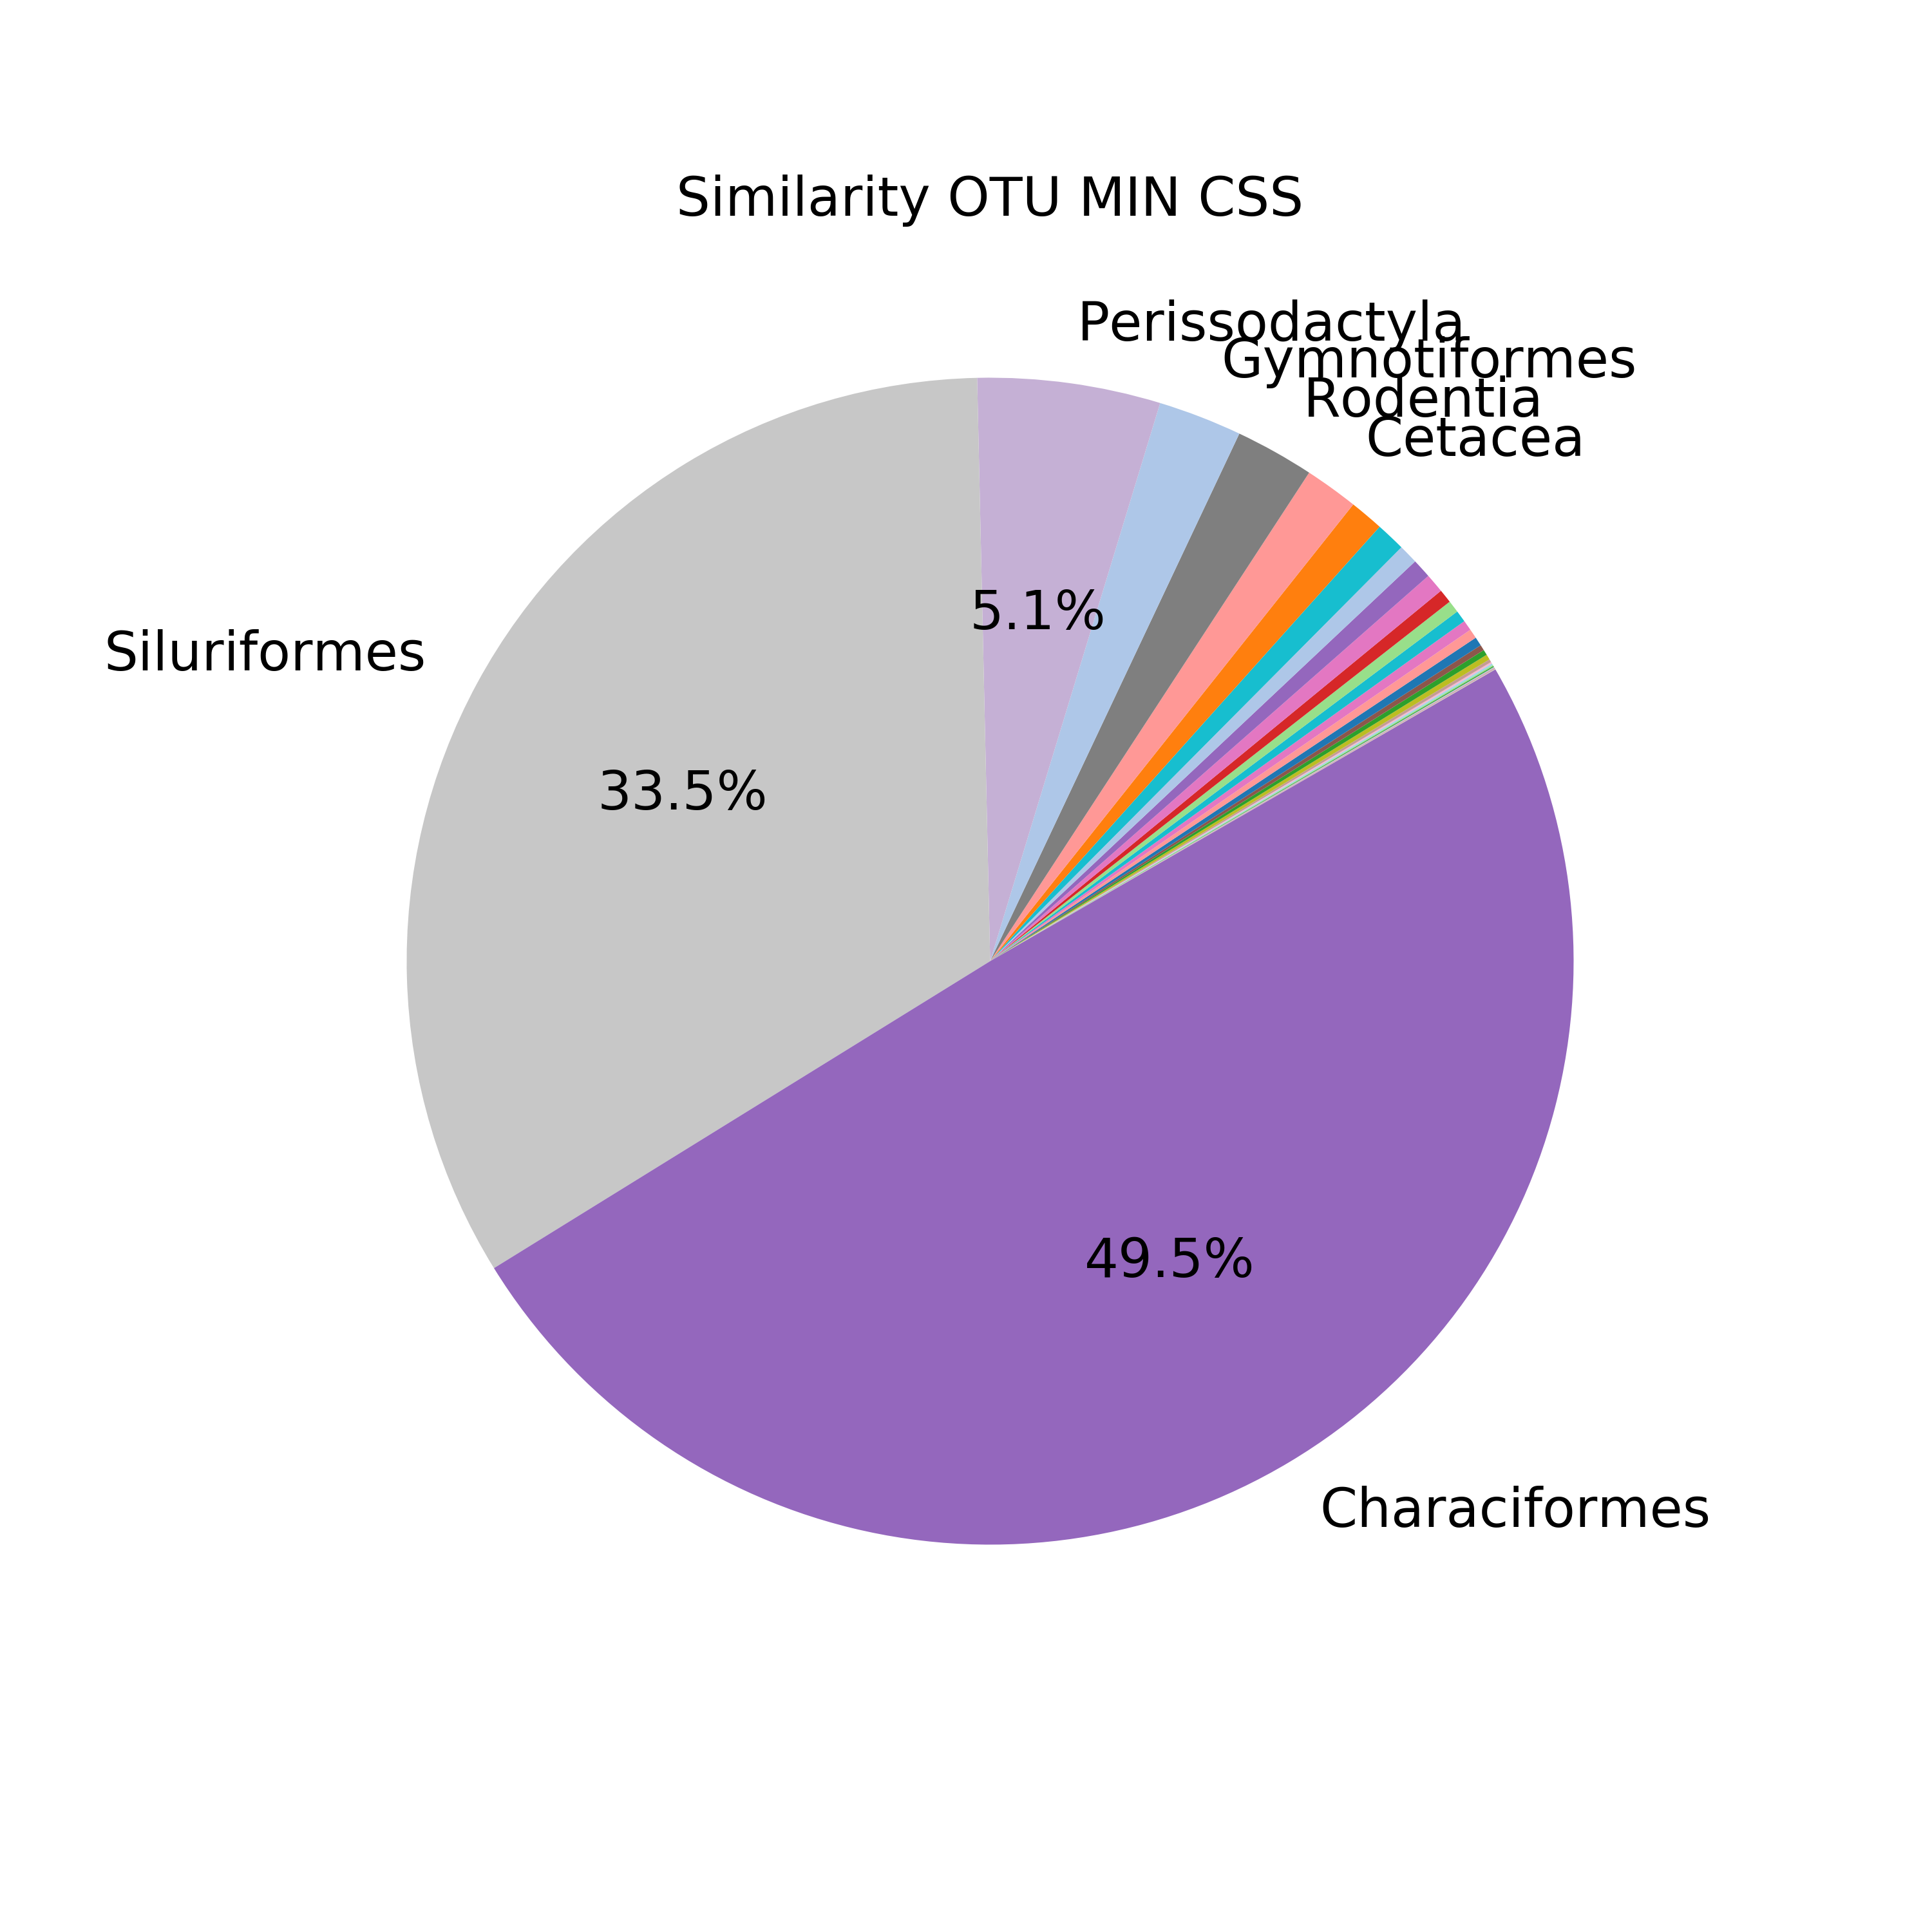
\includegraphics[width=\textwidth]{rfr_sim_sum_pieOTU MIN CSS}
		\caption{}
		\label{fig:simotumincsssum}
	\end{subfigure}
	\caption{Species' importance per taxonomic order as calculated by Random Forest in the maximum similarity test. Averaging the importance for the sets: OTU \ref{fig:simotumean}, and OTU MIN CSS \ref{fig:simotumincssmean}. Summing the importance for the sets: OTU \ref{fig:simotusum}, and OTU MIN CSS \ref{fig:simotumincsssum}.  }
	\label{fig:simpieappendix}
\end{figure}

\begin{figure}[h]
	\centering
	\begin{subfigure}{0.45\textwidth}
		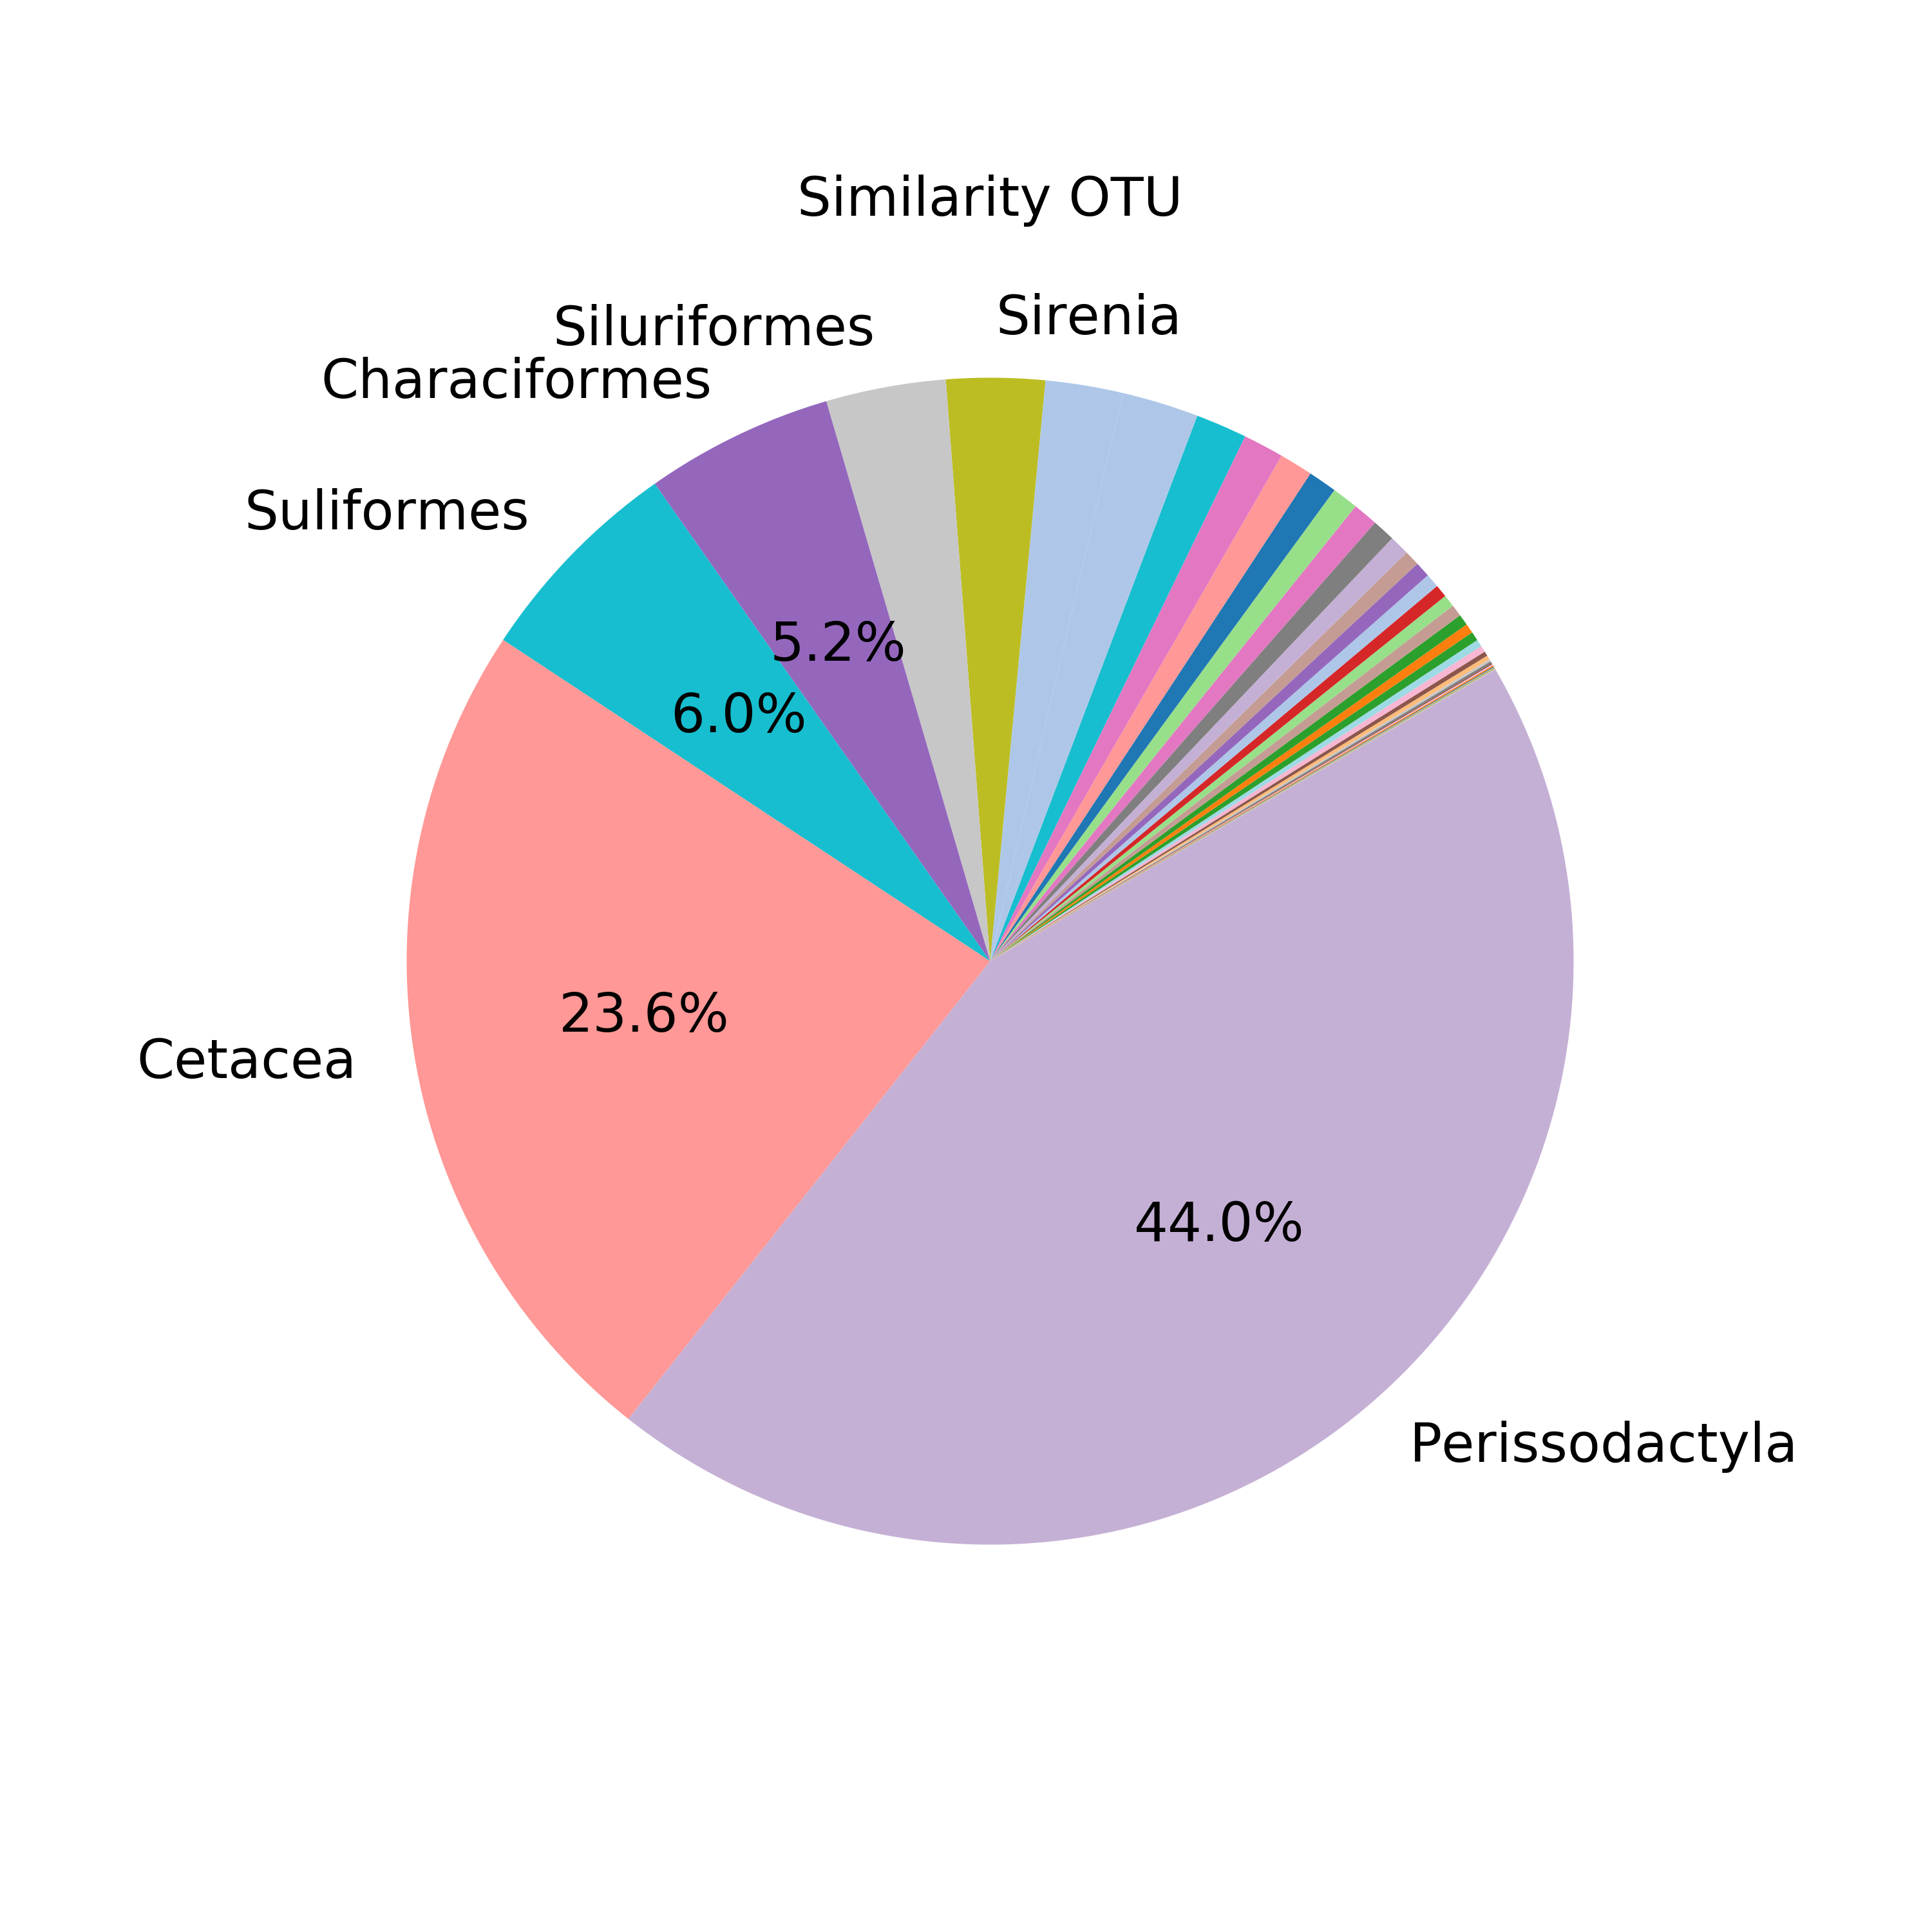
\includegraphics[width=\textwidth]{rfr_dis_mean_pieOTU}
		\caption{}
		\label{fig:dissimotumean}
	\end{subfigure}	
	\begin{subfigure}{0.45\textwidth}
		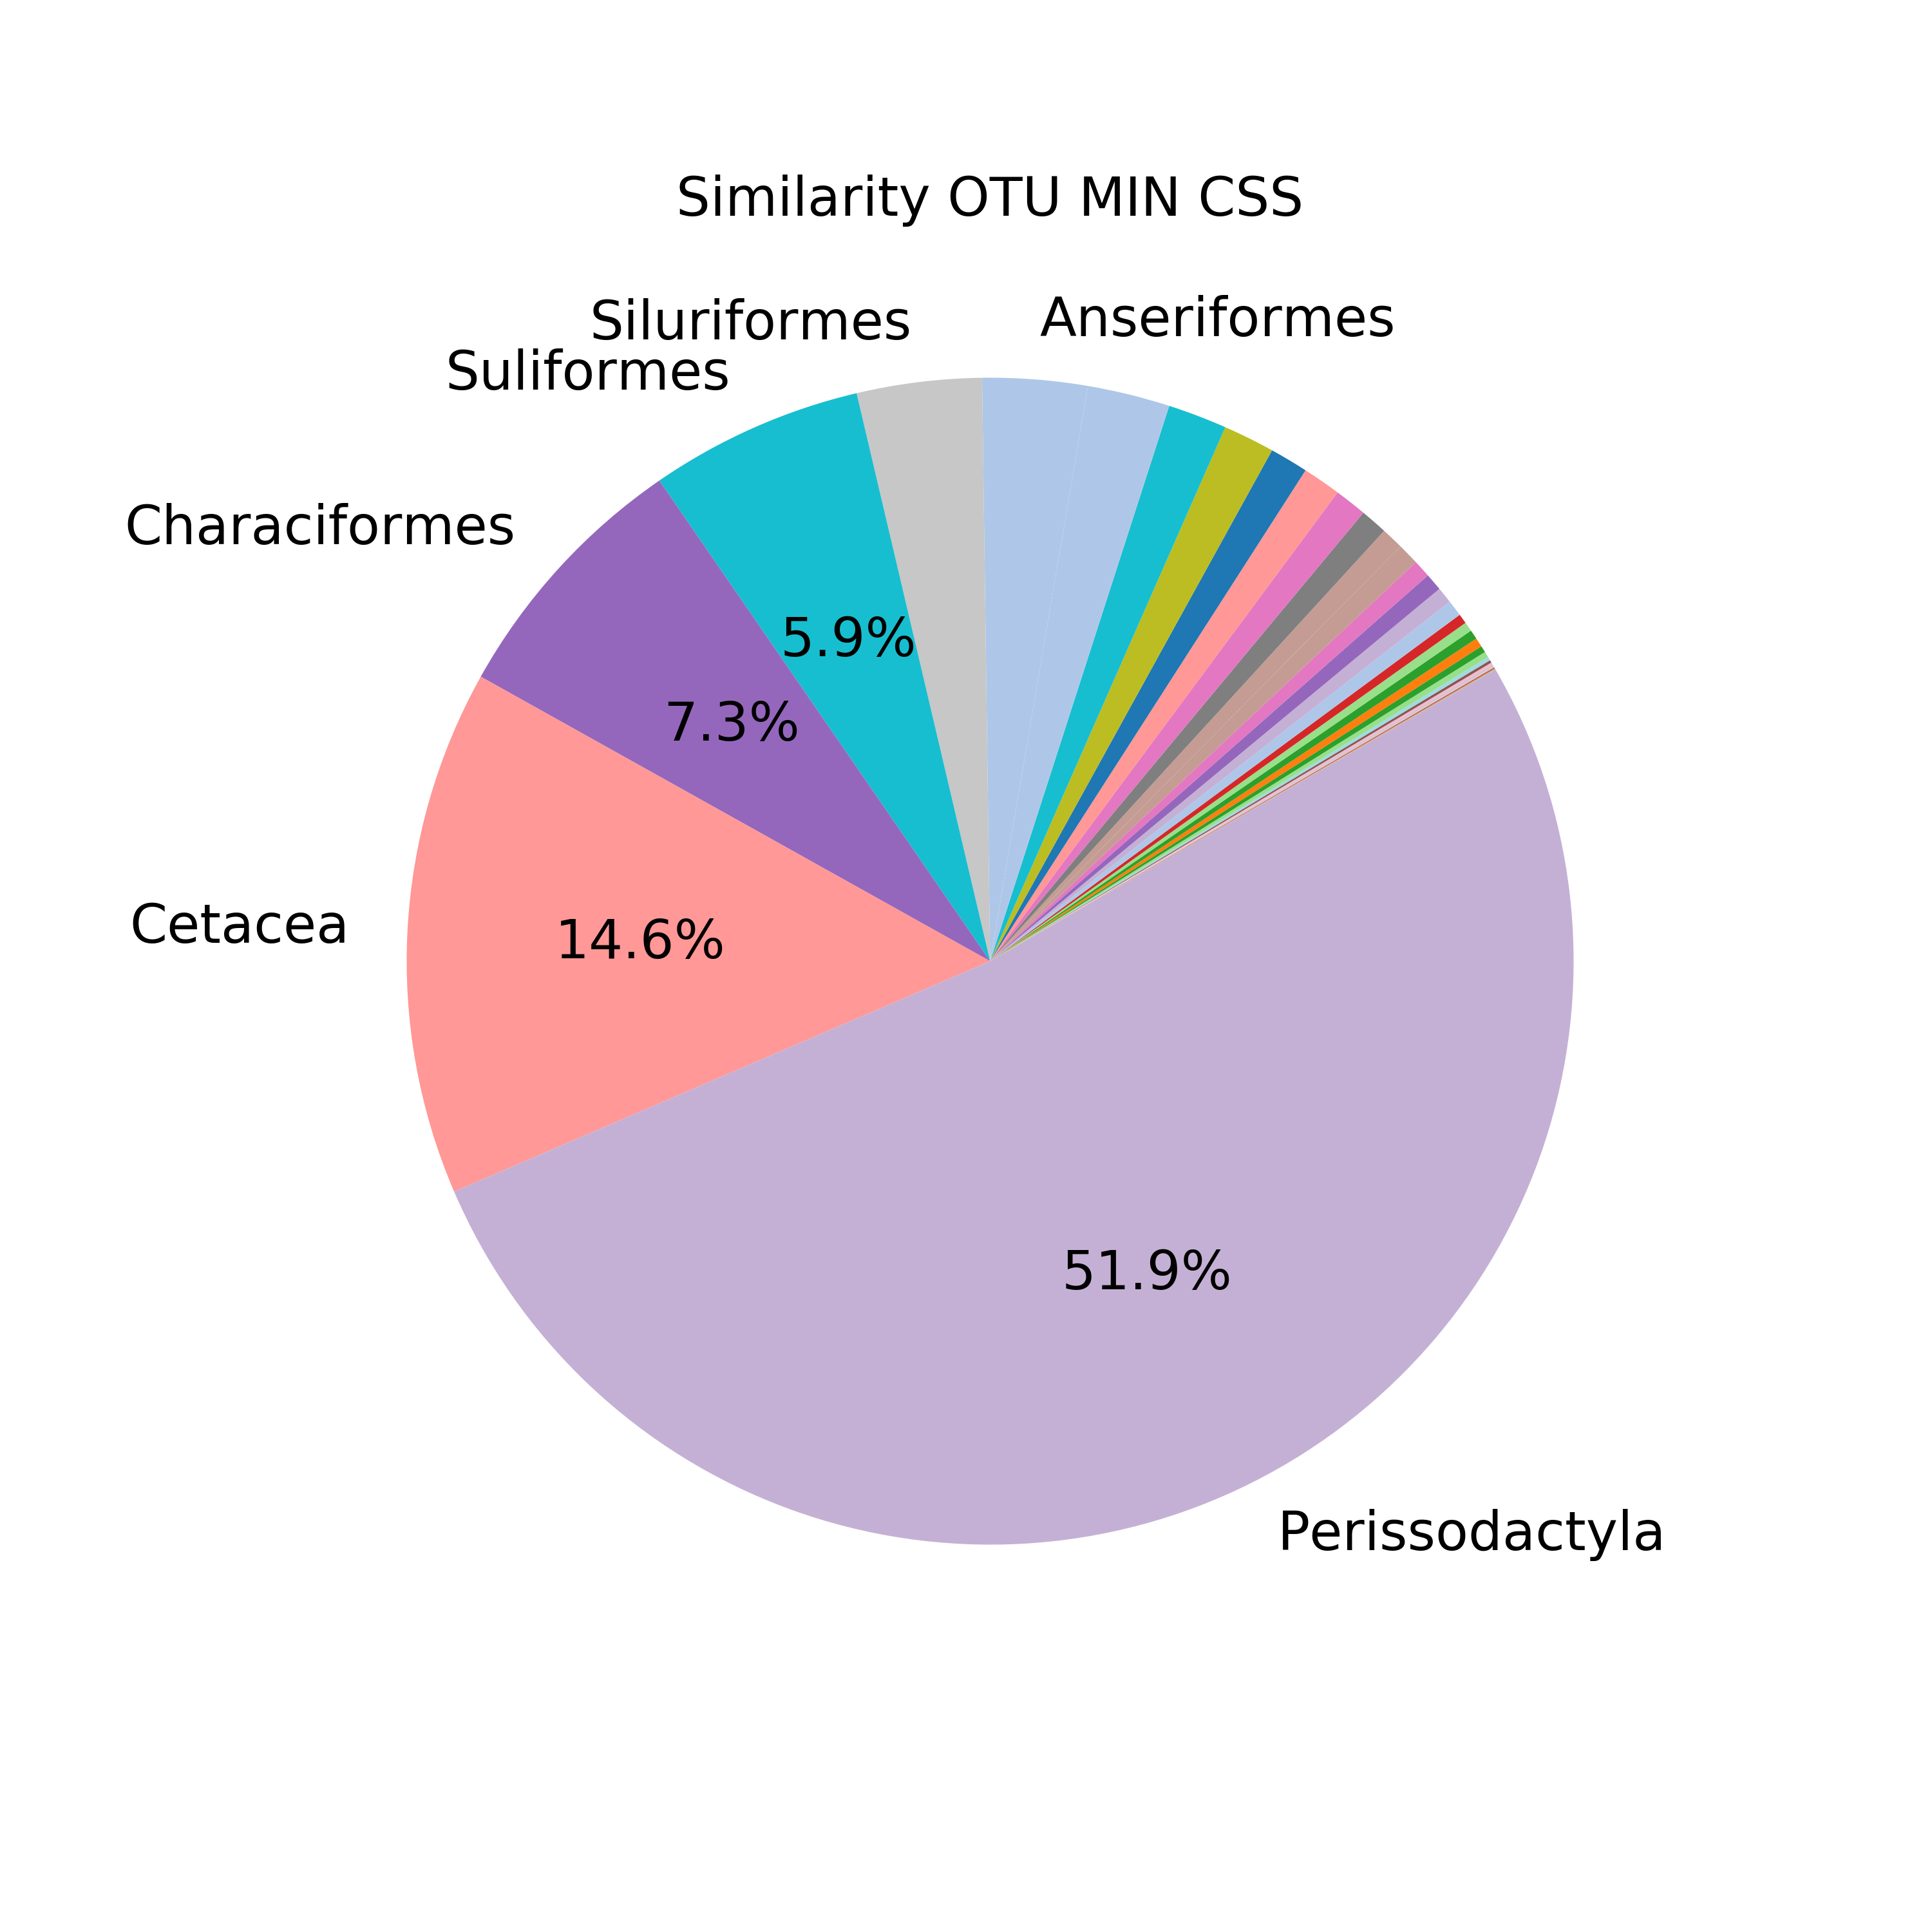
\includegraphics[width=\textwidth]{rfr_dis_mean_pieOTU MIN CSS}
		\caption{}
		\label{fig:dissimotumincssmean}
	\end{subfigure}\\
	\begin{subfigure}{0.45\textwidth}
	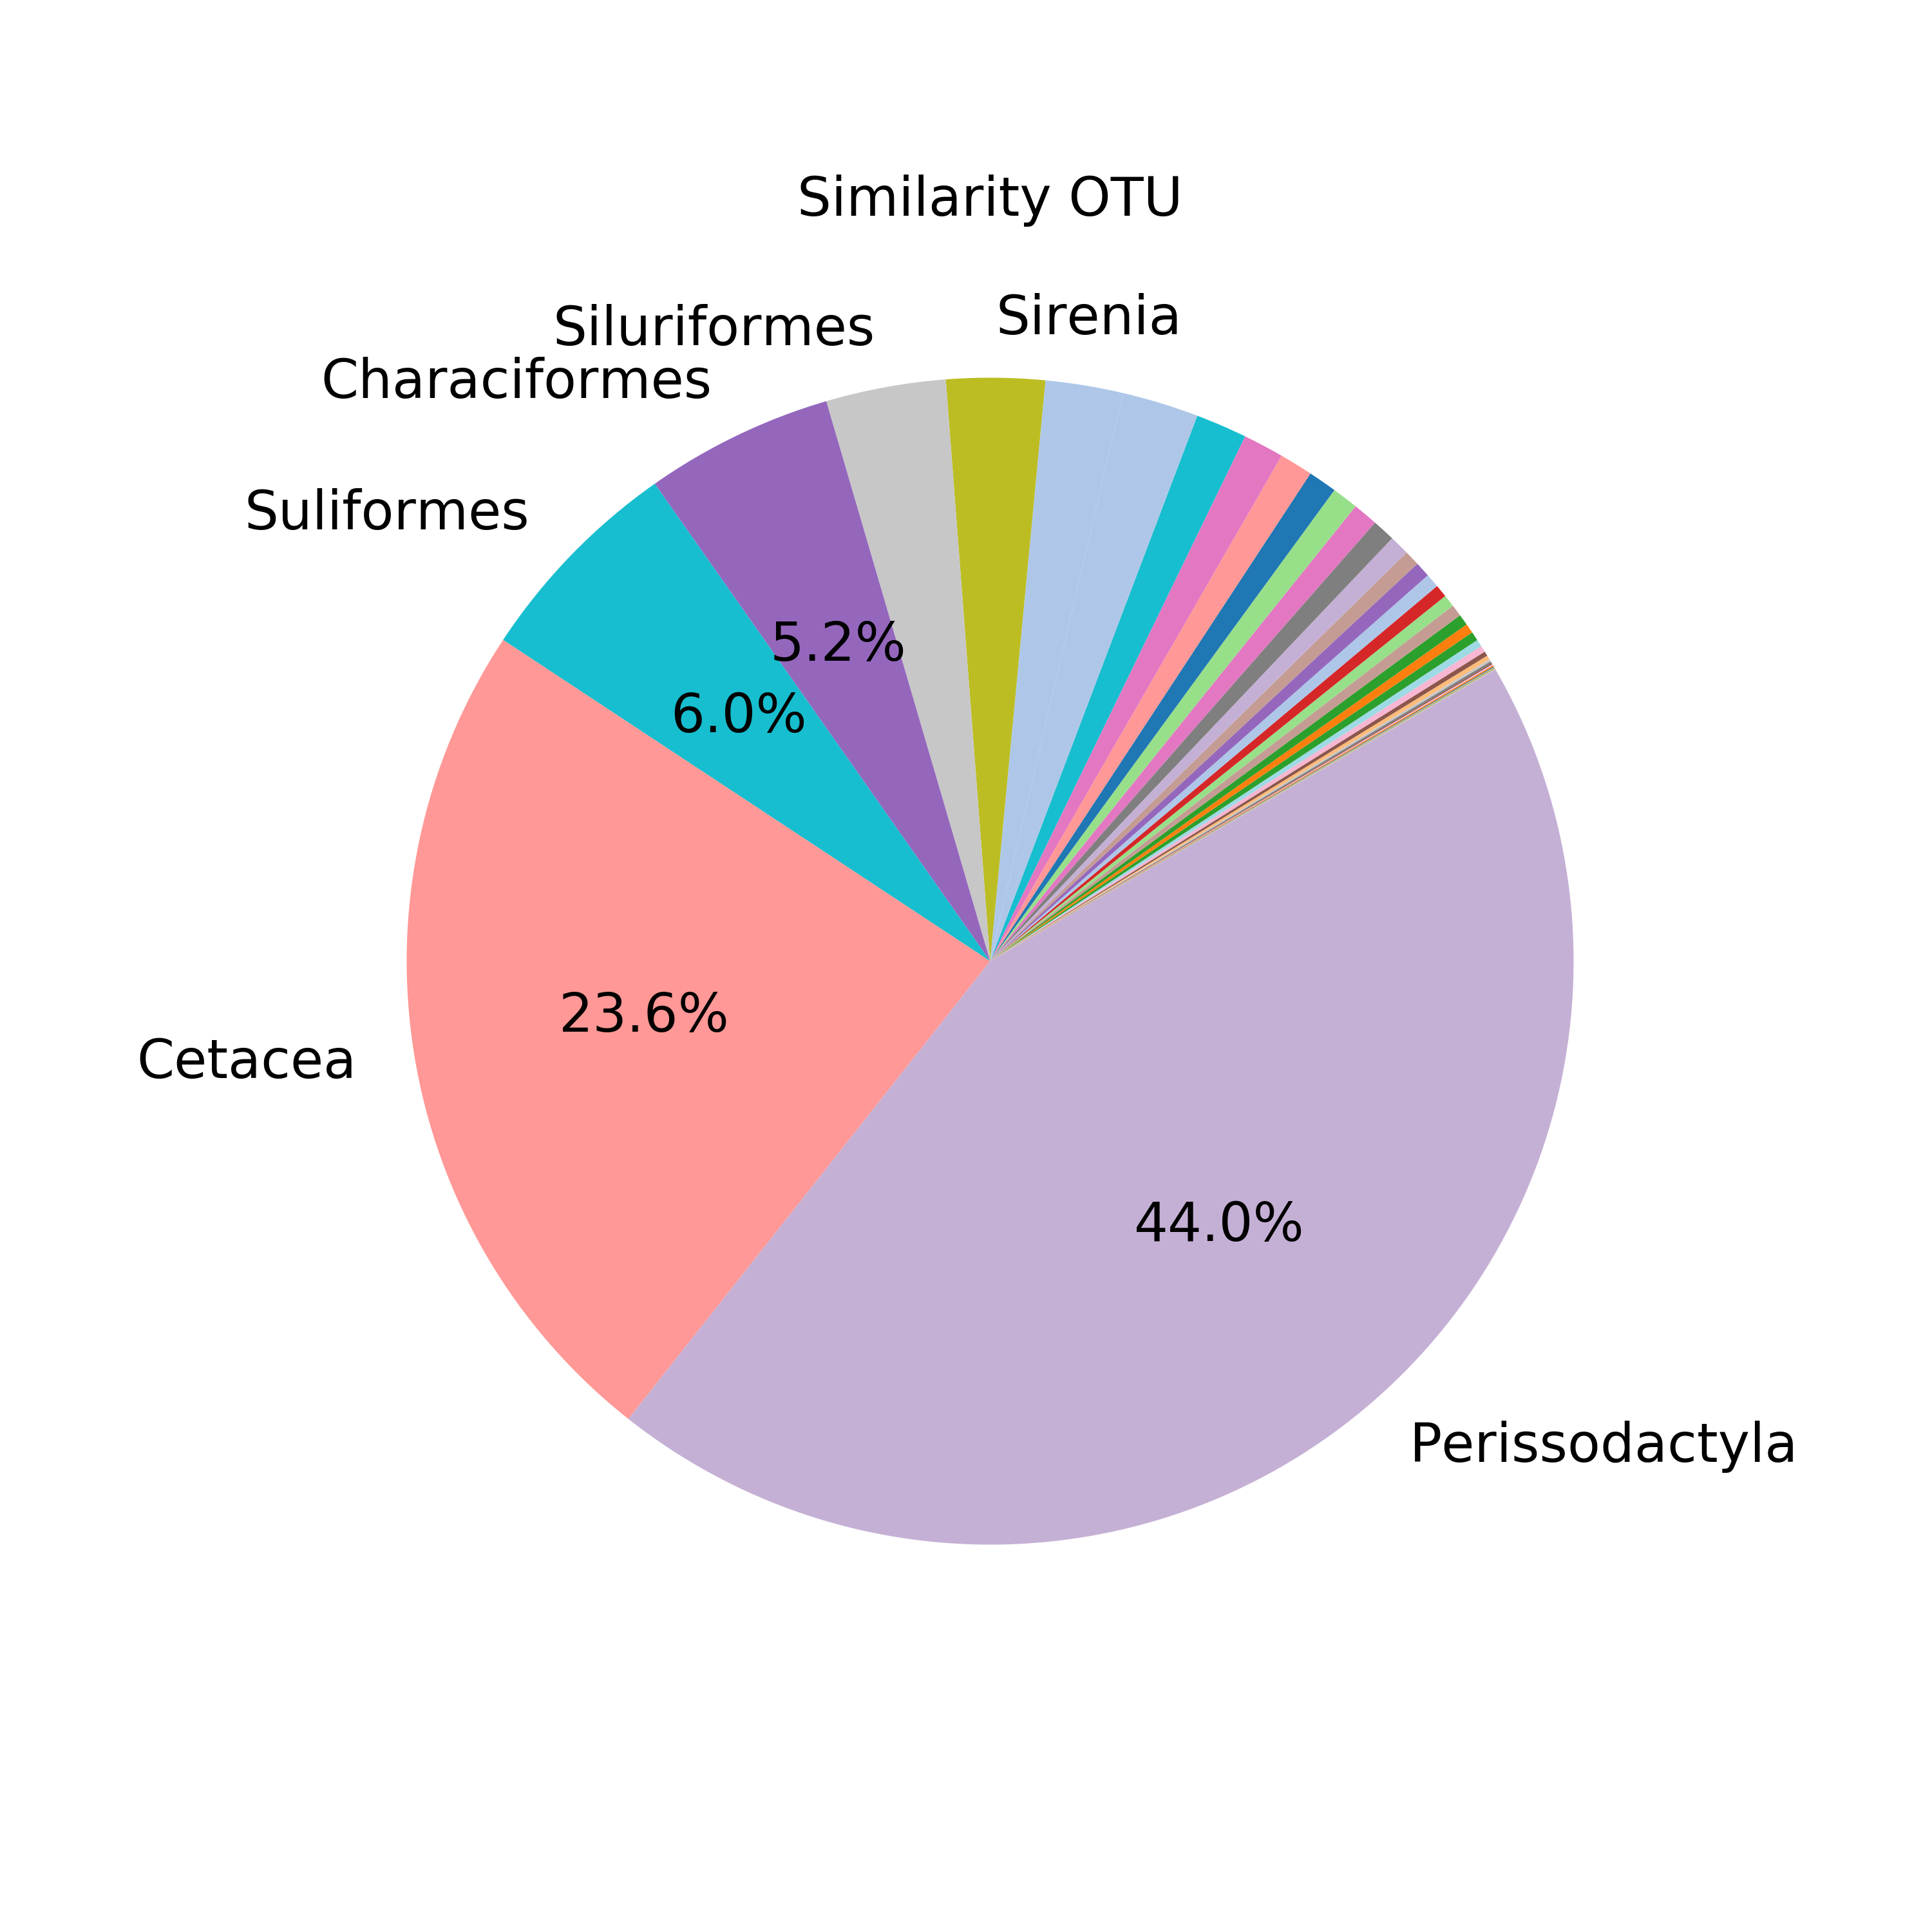
\includegraphics[width=\textwidth]{rfr_dis_sum_pieOTU}
	\caption{}
	\label{fig:dissimotusum}
\end{subfigure}	
\begin{subfigure}{0.45\textwidth}
	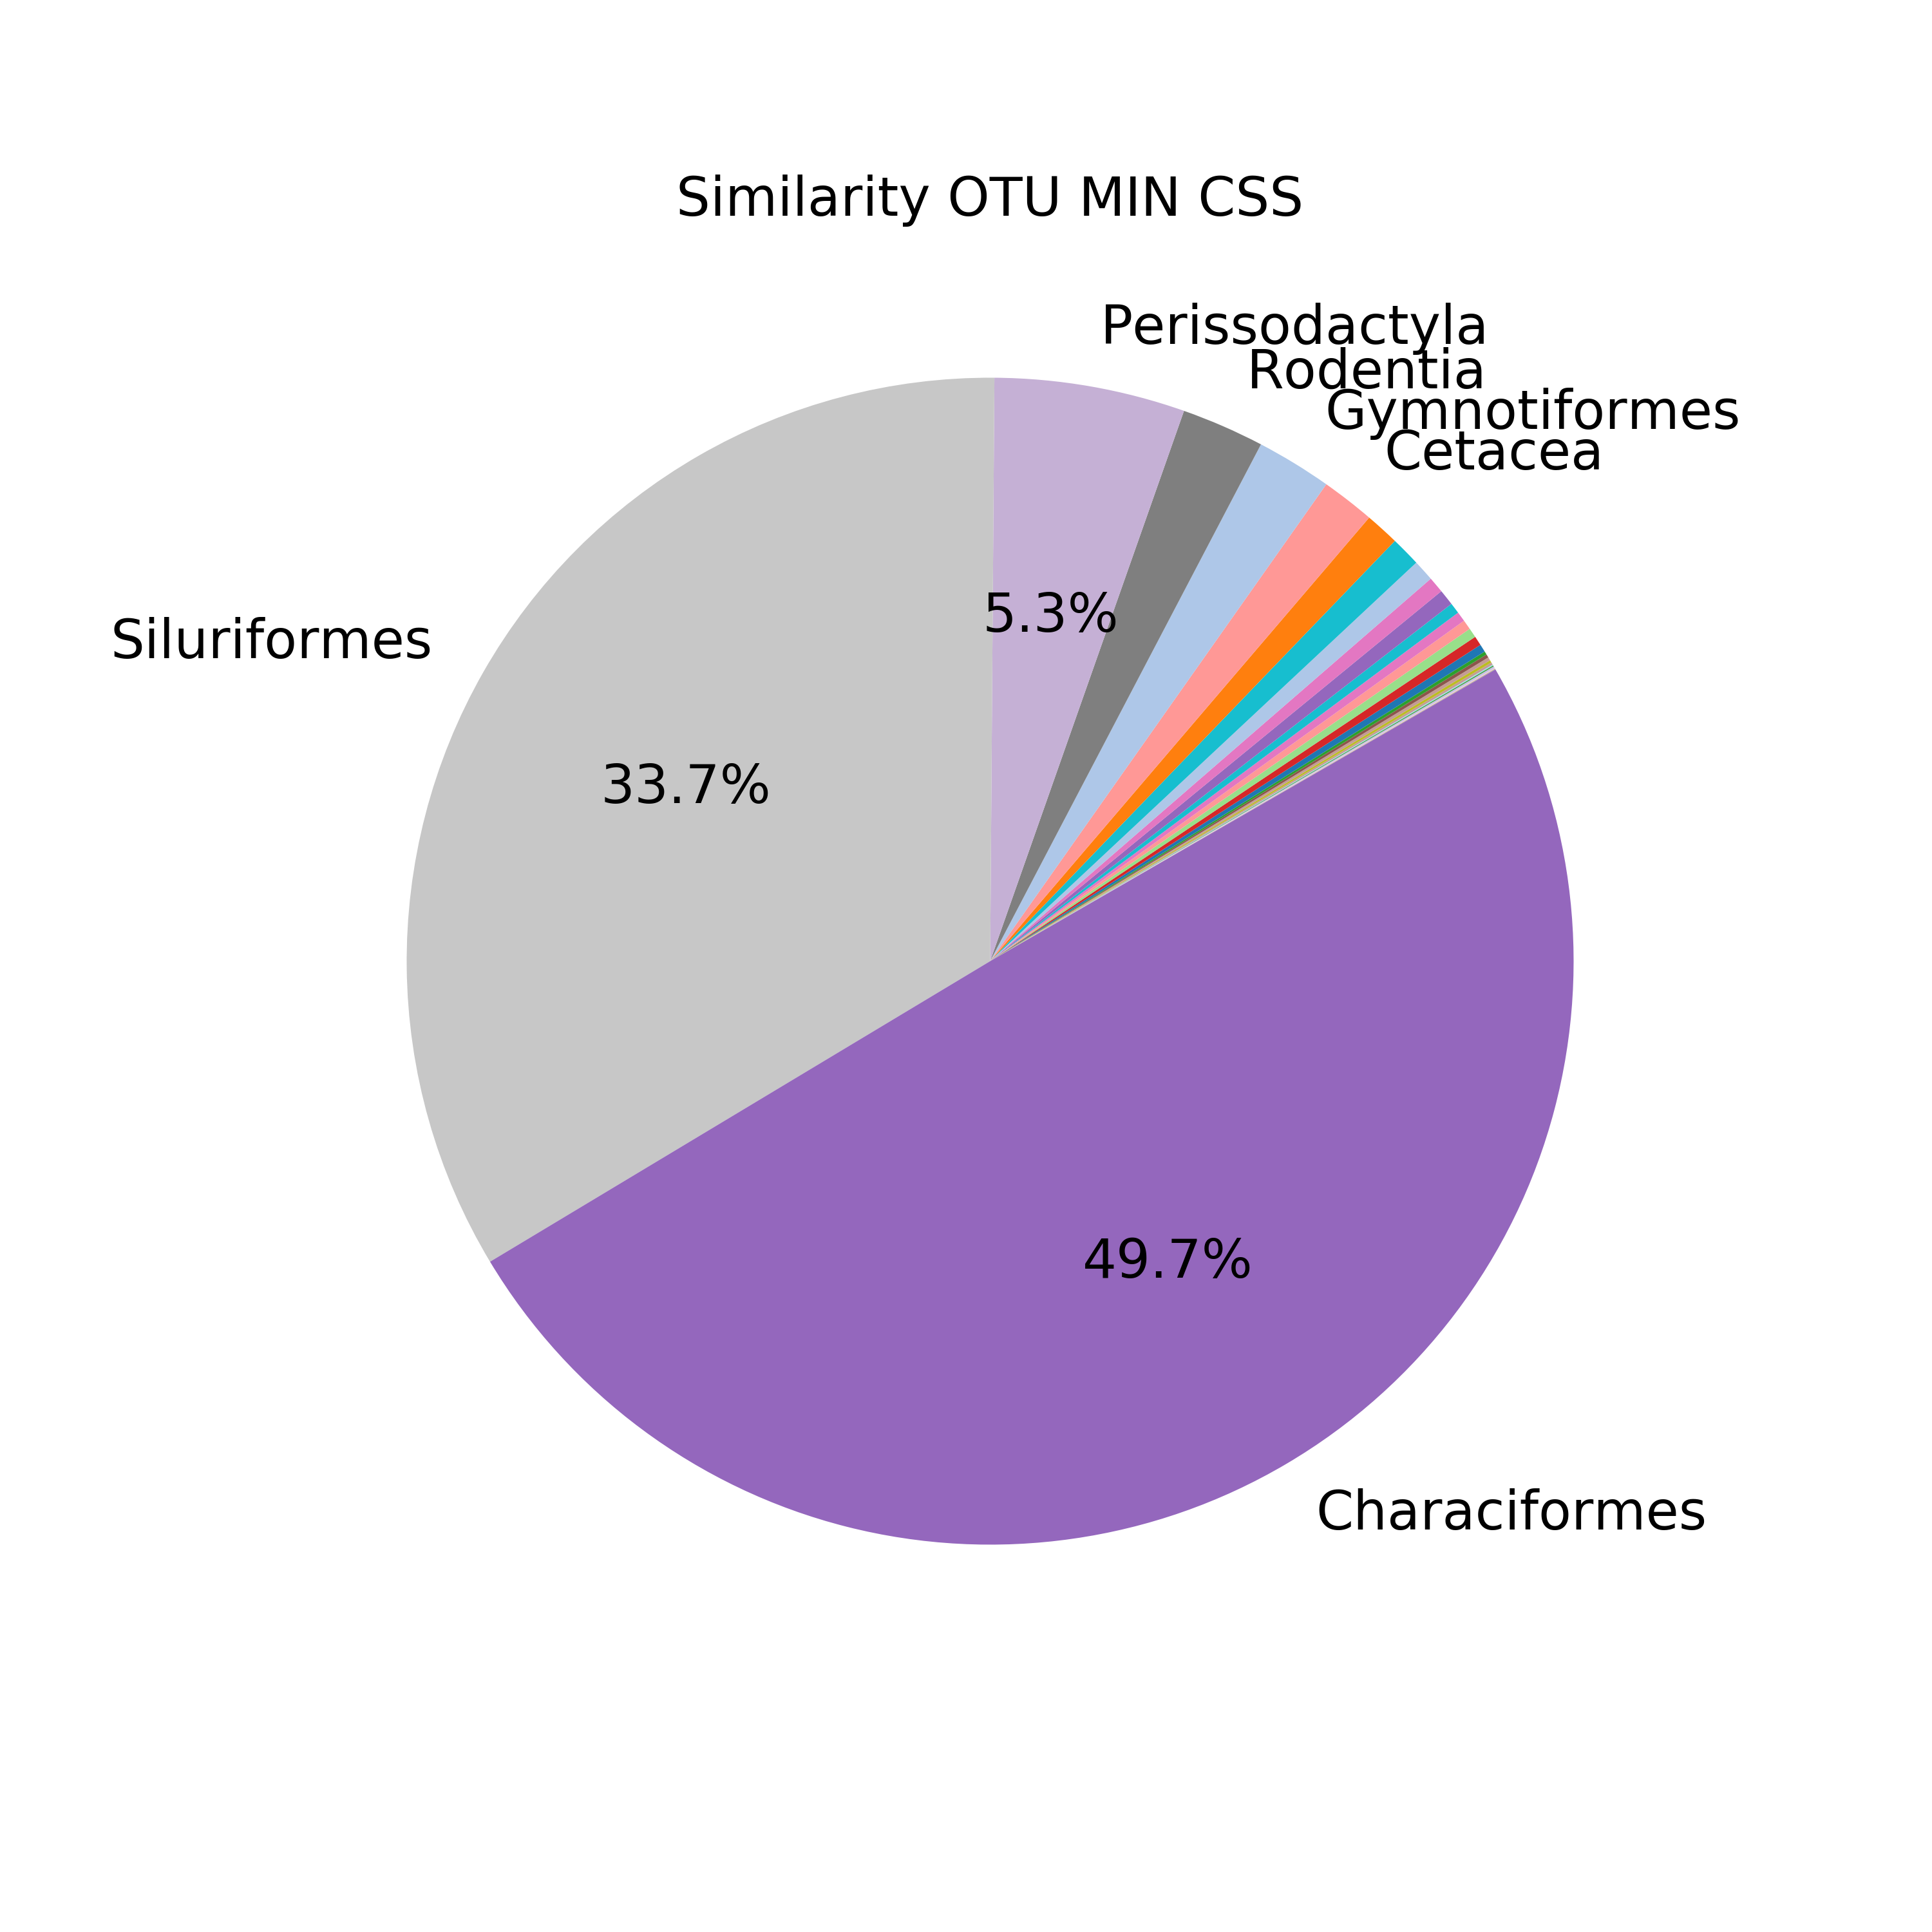
\includegraphics[width=\textwidth]{rfr_dis_sum_pieOTU MIN CSS}
	\caption{}
	\label{fig:dissimotumincsssum}
\end{subfigure}
	\caption{Species' importance per taxonomic order as calculated by Random Forest in the maximum similarity test. Averaging the importance for the sets: OTU \ref{fig:dissimotumean}, and OTU MIN CSS \ref{fig:dissimotumincssmean}. Summing the importance for the sets: OTU \ref{fig:dissimotusum}, and OTU MIN CSS \ref{fig:dissimotumincsssum}. }
	\label{fig:dispieappendix}
\end{figure}
%
%\subsubsection*{Debian/Ubuntu:}
%\begin{verbatim} 
%sudo apt-get install texlive texlive-latex-extra 
%sudo apt-get install psutils
%\end{verbatim}

%%!TEX root = ../thesis.tex
% ******************************* Thesis Appendix B ********************************

\chapter{Installing the CUED class file}

\LaTeX.cls files can be accessed system-wide when they are placed in the
<texmf>/tex/latex directory, where <texmf> is the root directory of the user’s \TeX installation. On systems that have a local texmf tree (<texmflocal>), which
may be named ``texmf-local'' or ``localtexmf'', it may be advisable to install packages in <texmflocal>, rather than <texmf> as the contents of the former, unlike that of the latter, are preserved after the \LaTeX system is reinstalled and/or upgraded.

It is recommended that the user create a subdirectory <texmf>/tex/latex/CUED for all CUED related \LaTeX class and package files. On some \LaTeX systems, the directory look-up tables will need to be refreshed after making additions or deletions to the system files. For \TeX Live systems this is accomplished via executing ``texhash'' as root. MIK\TeX users can run ``initexmf -u'' to accomplish the same thing.

Users not willing or able to install the files system-wide can install them in their personal directories, but will then have to provide the path (full or relative) in addition to the filename when referring to them in \LaTeX.

\end{appendices}

% *************************************** Index ********************************
%\printthesisindex % If index is present

\end{document}
